\documentclass[10pt]{book}

\usepackage[paperwidth=5in,paperheight=8in,includehead,
            inner=0.55in,outer=0.4in,top=0.56in,bottom=0.64in]{geometry}
\usepackage{amsmath}
\usepackage{amssymb}
\usepackage{graphicx}
\usepackage{adjustbox}
\usepackage[round,authoryear]{natbib}
\usepackage[hidelinks]{hyperref}
\usepackage{microtype}
\usepackage[most]{tcolorbox}
\usepackage{tikz}
\usetikzlibrary{arrows.meta,calc,bending,shapes.geometric}
% an inline regular polygon, for naming a rule by the cycle it closes rather
% than by the number of sides: \ngon{5} sets a small pentagon on the text line
% sized so that six sides can be told from seven at print resolution; smaller
% than this and the higher polygons all read as circles, which defeats the point
\newcommand{\ngon}[1]{\tikz[baseline=-0.75ex]{\node[regular polygon,
  regular polygon sides=#1, draw, minimum size=2.5ex, inner sep=0pt,
  line width=0.5pt] {};}}
% the two variants of L=2 do not lay down a cycle, so they cannot be named by
% one: the chorded rule's footprint is K_4 minus an edge, whose shortest cycle
% is a triangle, and the other's is a square with a link running off it
\newcommand{\sqdiag}{\tikz[baseline=0.5ex]{%
  \draw[line width=0.5pt] (0,0) rectangle (1.8ex,1.8ex);
  \draw[line width=0.5pt] (0,0) -- (1.8ex,1.8ex);}}
\newcommand{\sqstub}{\tikz[baseline=0.5ex]{%
  \draw[line width=0.5pt] (0,0) rectangle (1.8ex,1.8ex);
  \draw[line width=0.5pt] (1.8ex,1.8ex) -- ++(0.9ex,0.55ex);}}

% Compact running heads that fit the narrow 5x8 page.
\usepackage{fancyhdr}
\pagestyle{fancy}
\fancyhf{}
\fancyhead[LE,RO]{\small\thepage}
\fancyhead[RE]{\small\nouppercase{\leftmark}}
\fancyhead[LO]{\small\nouppercase{\rightmark}}
\renewcommand{\headrulewidth}{0.3pt}
\fancypagestyle{plain}{\fancyhf{}\renewcommand{\headrulewidth}{0pt}\fancyfoot[C]{\small\thepage}}

% Make the blank verso pages inserted before each chapter truly blank (no header).
\makeatletter
\def\cleardoublepage{\clearpage\if@twoside\ifodd\c@page\else
  \hbox{}\thispagestyle{empty}\newpage\if@twocolumn\hbox{}\newpage\fi\fi\fi}
\makeatother
% Grayscale palette (the book is printed in black and white).
\colorlet{accent}{black!80}
\colorlet{accentB}{black!50}

% Looser float placement so figures do not leave near-empty pages on the small trim.
\renewcommand{\topfraction}{0.9}
\renewcommand{\bottomfraction}{0.8}
\renewcommand{\textfraction}{0.07}
\renewcommand{\floatpagefraction}{0.7}
\setcounter{topnumber}{2}
\setcounter{totalnumber}{3}

% Skippable "calculation" box. Usage: \begin{calculation}{what is being computed} ... \end{calculation}
\newtcolorbox{calculation}[1]{%
  breakable,
  enhanced,
  colback=black!4,
  colframe=black!45,
  boxrule=0.5pt,
  arc=2pt,
  left=6pt,right=6pt,top=6pt,bottom=6pt,
  fonttitle=\bfseries\small,
  fontupper=\small,
  coltitle=black,
  title={The mathematics behind it: #1 \hfill\textnormal{\itshape(this box can be skipped)}},
}

% Dirac notation for the quantum-walk chapter. Defined here rather than pulled in
% with braket or physics, both of which redefine more than this book wants.
\newcommand{\ket}[1]{\lvert #1 \rangle}
\newcommand{\bra}[1]{\langle #1 \rvert}
\newcommand{\braket}[1]{\langle #1 \rangle}

% TeX breaks this one as "pseud-ofractal" if left to itself, and it appears
% often enough in chapters 6 and 7 to be worth telling it where the seams are.
\hyphenation{pseudo-frac-tal pseudo-frac-tals}

\pagenumbering{gobble}

\begin{document}

\title{Local network growth:\\How simple rules drive network complexity}

\author{Alexei Vazquez}
\maketitle

\thispagestyle{empty}
\vspace*{\fill}
\begin{center}
{\itshape To the ICTP, where it all started\ldots\\[0.7em]
and Nodes \& Links, for a renaissance.}
\end{center}
\vspace*{\fill}
\clearpage

\chapter*{Preface}

In the year 2000 I was at the International Centre for Theoretical Physics 
(ICTP), located in Trieste, Italy. I had left my home country, Cuba, and gone 
there, with many dreams and much nostalgia. At the ICTP I indulged myself in 
the library, the scientific meetings, the computer cluster, and new friends. 
Then, on May 22--25, 2000, I attended the Research Workshop on Graph Theory 
and Statistical Physics. There was a presentation by an obscure Hungarian 
physicist by the name of Albert-L\'aszl\'o Barab\'asi: ``Emergence of scaling 
in complex networks.'' A small conference room and few attendees. Yet, it was 
eye-opening, a fascinating introduction to the properties of real networks 
and a hypothesis for their evolution. When I left that room I was charged, 
full of ideas. Two weeks later I had my first paper on network science: 
``Knowing a network by walking on it: emergence of scaling'' 
\citep{vazquez2000walk}. And right there, it all started.

Networks are everywhere, and so are the regularities they share. Whether one
looks at the Internet, the World Wide Web, a society, a cell, or the scientific
literature, the same statistical signatures recur: broad, often scale-free
degree distributions; short distances between nodes; high local clustering that
thins out in a regular hierarchy as degree grows; and systematic correlations
between the degrees of neighboring nodes. That these features appear across
systems with nothing else in common is one of the most striking findings of
network science. Explaining them has been the field's central occupation for
more than two decades.

The dominant explanation has rested on the preferential attachment mechanism, 
proposed by R\'eka Albert and Barab\'asi \citeyearpar{barabasi1999}: new nodes connect to existing ones
in proportion to their degree, and a power law follows. It is a powerful 
idea, but taken literally it is a \emph{global} rule, requiring each newcomer 
to weigh every node in the network against every other. Real web pages, 
proteins, and people do no such thing. They act on what is near them --- the 
page a surfer reaches, the friend a friend introduces, the gene that gets 
copied. Preferential attachment is a macroscopic perception. In the same way, our perception of temperature is a macroscopic consequence of air molecules heating our skin. This book is about the microscopic mechanism behind 
preferential attachment and beyond: the regularities of real networks 
\emph{emerge} from local rules. A growth rule that reaches just one step 
beyond a randomly chosen node, to one of its neighbors, already attaches 
preferentially by degree --- and the same locality that produces preferential 
attachment produces the clustering hierarchy, the degree correlations, the 
community structure, and the multiplicity of shortest paths, all as a 
package. Coincidentally, I consolidated these ideas while working as a postdoctoral research associate in Barab\'asi's group, then at the University of Notre Dame.

The chapters develop this thesis one mechanism at a time. After an introduction
that fixes the measures and states the argument, I treat growth by search
(citation and web graphs), by triadic closure (social networks), and by
duplication (protein interaction networks) --- the three local rules of my 2003
paper --- and then carry the same principle into more recent work: the
duplication--split structure of project schedules, the emergence of communities
from local rules, the vocabulary in which that structure is best described, and the
boosting of shortest path multiplicity. Two closing chapters put a walker back on the
networks the rules built. The first lets it diffuse, and reads the scales of a network
off the thermodynamics of that spreading; the second makes it quantum, so that unlike
the classical walker of Chapter~\ref{ch:search} it never forgets where it started,
and finds the growth rule legible in how far it can travel. Each chapter
pairs a concrete local rule with a class of real networks it illuminates, and
each ends where it began, with the conclusion that locality is the common cause.

The book is intended for anyone curious about how complex systems organize 
themselves --- the interested general reader as much as the specialist. 
Readers drawn to the \emph{general} principle will find it running through 
every chapter. Mathematicians, computer scientists, and physicists, in 
particular, will recognize a single idea applied again and again: that a 
handful of simple local rules, with no global coordination, is enough to 
account for the statistics that recur across otherwise unrelated networks; 
the closing chapters on the emergence of communities and on the redundancy of 
shortest paths push that idea furthest. Readers drawn instead to a 
\emph{particular} system will find it given a chapter of its own. Social 
scientists will recognize their networks of acquaintance and collaboration in 
the friends-of-friends mechanism of Chapter~\ref{ch:friends}; biologists will 
find the evolution of protein interaction networks through gene duplication 
in Chapter~\ref{ch:duplication}; project managers and engineers will find the 
anatomy of project schedules --- and the surprising irrelevance of the 
critical path --- in the activity-specialization model of 
Chapter~\ref{ch:projects}; and those who study the web, citation, or the 
spread of information online will find the search-and-connect rule of 
Chapter~\ref{ch:search}. Graduate students entering the field will find the 
models developed in full. Whatever the entry point, the core ideas are told 
in plain language, and the more technical calculations are set in boxes that 
can be skipped without losing the thread. I have tried to keep the analysis 
self-contained, favoring mean-field arguments that make the mechanisms 
transparent over exhaustive rigor, and to let the empirical data set the 
agenda throughout. Readers will find the degree denoted $k$, the elements of 
a graph called nodes, and their relations called links, following the 
now-standard usage of network science.

Much of this material grew out of collaborations and conversations over many 
years, with special mentions to Alessandro Vespignani, Yamir Moreno, Romualdo 
Pastor-Satorras, Amos Maritan, Alessandro Flammini, Albert-L\'aszl\'o 
Barab\'asi, Sara Nadiv Soffer and Christos Ellinas. The original research 
papers on which the chapters draw are cited at the appropriate points and 
collected in the bibliography. Parts of the prose, and several of the 
figures, were prepared and edited with the help of Anthropic's Claude 
(Opus~4.8). I am grateful to the colleagues who shaped these ideas, and to 
the reader who, I hope, will come away persuaded that complex networks need 
not be designed --- that they can grow themselves, one local decision at a
time.

\emph{A note on the second edition.} The first edition argued its case largely
through models and mean-field reasoning; this one holds the models up to the
world. Real networks now run through the book --- drawn from public repositories
and measured with standard tools --- beginning in the introduction, where the
recurring regularities are shown in data rather than only described, and where a
closer look finds that one of them, the clustering hierarchy, is in good part an
artifact of how it is usually measured. The two closing chapters have grown the
most. The chapter on communities now makes exactly solvable, for several
idealized networks, the question of \emph{when} a network acquires communities,
and ends by measuring across close to a hundred real networks how their
\emph{number} grows with size; the chapter on shortest paths gains a mean-field
theory of redundancy and two constructions solved in closed form. Throughout, new
figures --- the first plots of real data in the book, alongside fresh schematics
--- aim to make the ideas visible as well as legible. The thesis is unchanged; the
evidence for it is stronger.

\emph{A note on the third edition.} The second edition ended its chapter on
communities with a number: the count of communities grows as a power of network
size, with an exponent above the self-similar one half. Three new chapters ask
what that number is a number \emph{of}, and the answer turns out to depend less
on the networks than on the instrument.

The first of them replaces the flat description of communities with a
\emph{nested} one, in which the groups are themselves grouped --- communities of
communities, the block structure described by a block model of its own rather
than spelled out entry by entry. That sounds like a technicality and is not. A
flat description pays a charge growing with the square of the number of groups,
and so cannot report more than about $\sqrt{n}$ of them however many are there;
and $\sqrt{n}$ is precisely the self-similar benchmark the measured exponent was
being held against, so the instrument could not have returned a value far above
it even in principle. Lift that ceiling and the exponent goes from two thirds to
one. The number of communities grows in proportion to size, their typical size
stops growing, and what a locally grown network converges to is not a shape at
all but a density --- so many communities per node, constant as the network grows
and set by the rule that grew it. That is the second edition's power law resolved
into something a network simply has, the way it has a clustering coefficient. It
comes with a caution the same chapter supplies: of the hierarchy such a fit
reports, only the bottom level is a measurement, and the tidy branching above it
is the prior's own scaffolding.

The other two chapters ask what the describer may \emph{name}. Giving the model a
vocabulary that can call a set of links a triangle or a square, rather than only
a pair of endpoints, can remove the communities altogether --- on networks whose
communities the second edition had proved exist. And on the two lattices whose
best description can be written down by hand rather than searched for, the
fitting misses it, by a tenth of the description length; there is no better cure
for confidence in one's own numbers than a case where the answer can be checked.

What emerges from following that is a single object rather than two. A network
motif and a network community are the same thing at two scales --- both say that
a set of nodes belongs together and how it is joined, the motif from a template
fixed in advance, the community bespoke and inferred --- and once they are
counted together, the quantity that survives every change of instrument is the
density of the two combined, constant in size and set by the growth rule. Local
rules do not converge to a shape that can be drawn. They converge to a rate at
which they keep writing structure, and the argument over how much of that
structure is ``motif'' and how much is ``community'' turns out to be an argument
about vocabulary. The three chapters are the case for that, and they are also, I
hope, an honest record of how often the instrument had to be rebuilt before the
measurement meant anything.

\emph{A note on the fourth edition.} The third edition ended by claiming that what a
locally grown network converges to is a density of meso-structure --- motifs and
communities counted together, so many per node, constant as the network grows. The
claim was won by an argument about description length: about what it costs to transmit
a network, and which vocabulary transmits it cheapest. That leaves an obvious
objection, and it is the right one to press. A statement about the cheapest
description is a statement about descriptions. Is there anything in the network
itself?

This edition adds two chapters, and both answer that by putting a physical probe on
the same networks and asking it. The probes are walkers. Neither can fit a model,
choose a prior, infer a number of blocks, or decide whether to call four links a
square; both can only move, and one watches where they get to.

The first walker is the ordinary one, diffusing. Treat the spread of heat over a
network as a Boltzmann weight and the diffusion time becomes a resolution knob, with
a specific heat that is flat where there is no scale to find and peaks where there is
one --- and whose height, it turns out, is the dimension the diffusion sees. On a
ring that reads one, as it must. On the diamond lattice of Chapter~\ref{ch:communities}
it becomes something better: the specific heat announces one peak per generation of
the construction, spaced by a factor this book can derive, and the whole ladder
oscillates around a plateau fixed by the lattice's parameters. That chapter's real
payoff is a comparison. Chapter~\ref{ch:communities} built a renormalization group
for the diamond out of counting links; the diffusion gives a second one, out of
spreading over it, and the two differ by exactly one power --- structure rescales
length, diffusion rescales time, and on this lattice time is length squared. Two
renormalization groups on one object, agreeing in a way that can be written down.
Against that I have to set what the same instrument cannot do: it does not tell the
book's growth rules apart, and it puts gene duplication and preferential attachment
on top of each other, which is the one pairing I would most like separated.

The second walker is quantum, and it is there because the first one always relaxes in
the end. It cannot fit a model either, but unlike the classical walker it never
forgets, so it can be confined for all time rather than merely delayed, and one can
measure how much of the network it ever reaches. The provocation was a paper of Lucas B\"ottcher and Mason
Porter \citeyearpar{boettcher2025localization}, who found such a walker trapped on
networks built by recursively attaching triangles and concluded that local clustering
is what traps it. Their triangles are this book's
triangles, so the result reads like a statement about this book, and testing it needed
only running their measurement on rules that separate clustering from everything it
travels with --- which is what four chapters of building limit classes and controls had
already produced.

Clustering turns out not to be the cause. The cleanest case is a single dial: the rule
that lays a chain of one node across a random link closes a triangle and has a
clustering coefficient of nearly three quarters, the same rule with a chain of two
closes a square and contains no triangle at all, and the two trap a walker equally
tightly. Nor is it the communities, which was my own first guess and is refuted by the
book's own controls --- of three rules that close the same square, the one with no
communities at any size is the one that traps hardest. What does predict the walker's
territory is the footprint of the rule, the plain size of the structure it keeps
building; and measured not in nodes but in units of meso-structure, that territory is
the same handful for every rule in a family across which it varies threefold in nodes.
The third edition's invariant, recovered by a route with no description length in it
anywhere. Two arguments this different agreeing is the best evidence I have that the
quantity is a thing and not an artifact of how it was found.

The chapter also ties the walker's confinement to the census exponent of
Chapter~\ref{ch:graphons}, predicting that a localization exponent should equal one
minus it, so that the fractal limit class Chapter~\ref{ch:motifs} defines and cannot
find has a second and physical way of being looked for. It stays empty. What the
prediction did not anticipate, and what only five octaves of size revealed, is that the
marginal case carries a logarithm: the rules with the loosest footprints do not
saturate but creep on like $\ln n$, slowly acquiring meso-structure as they grow. And
one rule turns out to trap by a mechanism with no geometry in it at all. Duplication
makes nodes with identical neighborhoods, identical neighborhoods are an exact
symmetry, and an exact symmetry forces eigenvectors of the walk living on two nodes.
That one is a theorem and not a measurement, which is what made it worth taking to real
data.

So the chapter ends where the duplication chapter always pointed, on real protein
interaction networks --- eight of them, drawn from a public repository and small enough
to diagonalize exactly. They are the most strongly localized networks in the book: a
walker on one reaches between two and seven proteins and no more, where the same walker
on a power grid or a road network of the same size and sparsity roams over fifteen or a
hundred and twenty-seven. And it is their wiring that does it, not their degrees ---
shuffle every link while keeping every protein's number of partners exactly, and the
confinement loosens in all eight, in one case by a factor of sixty-five. The
signature the theorem predicts is there too, in seven of the eight, on a scale that
cannot be accidental: between a third and three quarters of the whole spectrum sits at
one single eigenvalue. The eighth is the one network assembled by a different experiment
rather than a two-hybrid screen; it has no twins to speak of and is localized as hard as
any of them, so the symmetry is one way to trap a walker and not the only way --- which
is not something the models had suggested.

Whether that symmetry is duplication I could not establish, and the reason is worth
recording rather than burying. In these datasets a third to three fifths of proteins
have exactly one recorded partner, and two proteins that have been seen once each with
the same partner are indistinguishable from twins by any measure of topology. That is
what an unfinished experiment looks like as much as what a recent duplication looks
like. Counting only twins that share two or more partners --- which no single lucky
observation can manufacture --- what remains is a few per cent, and a few per cent
cannot be what traps the walker, even though a shuffled network almost never produces
it and so those twins are certainly real. The localization is measured, the theorem is
exact, and the link between them in living cells is not yet made. I have said so in
the chapter and named the two experiments that would decide it.

I have left in the negative results, the one rule I could not resolve, and the one test
whose result I do not trust --- merging the twins of a real interactome delocalizes it,
but the operation removes a third of the network along with the symmetry, and that is
not evidence. The chapter is shorter than the three that precede it and asks less of the
reader, but it does the thing those three could not: it takes a quantity that four
chapters arrived at by argument, and finds it again in something that moves.

\vspace{1em}
\noindent Alexei Vazquez

\tableofcontents

\chapter{Introduction}
\label{ch:introduction}

\setcounter{page}{1}
\pagenumbering{arabic}

\section{Networks everywhere}

Look closely at almost any complex system and you will find, hiding inside 
it, a network. A network, in the sense used throughout this book, is nothing 
more exotic than a collection of things together with a record of which pairs 
of them are connected. The ``things'' are drawn as dots and called 
\emph{nodes}. A connection between two of them is drawn as a line and called 
a \emph{link}. That is the whole vocabulary needed to begin: a network is 
dots and lines, nodes and links.

What is remarkable is how many different systems fit this simple picture. The 
Internet is a network whose nodes are routers and whose links are the cables 
between them. The World Wide Web is a network of pages connected by the 
hyperlinks you click. A society is a network of people connected by 
acquaintance, friendship, collaboration, or contact. A living cell contains a 
network of proteins connected when two of them physically interact, and 
another of chemicals connected by the reactions that turn one into another. A 
project is decomposed into discrete activities and the logical dependencies 
between them. The scientific literature is a network of papers connected by 
citations, and of authors connected when they write a paper together 
\citep{newman2001,newman2003,albert2002,dorogovtsev2002}. These systems share 
almost nothing on the surface --- one is silicon and glass, another is flesh 
and acquaintance, another is ink and ideas --- and yet, viewed as networks, 
they turn out to look astonishingly alike.

That likeness is the subject of this book. Over the past few decades, as
researchers gathered maps of real networks ranging from a handful of nodes to
billions, the same handful of features kept reappearing, no matter the system.
Four of them organize everything that follows, so it is worth meeting them in
plain language before we make them precise.

The first is the \emph{small-world} property \citep{watts1998}. In a real
network you can usually get from any node to any other in only a few hops, even
when the network is enormous --- the famous ``six degrees of separation'' between
any two people on Earth is one example. At the same time these networks are
highly \emph{cliquish}: your friends tend to be friends of one another, far more
than chance would predict. Short hops everywhere, plus dense little
neighborhoods: that combination is the small world.

The second is the \emph{scale-free} property \citep{barabasi1999,faloutsos1999}.
If you count how many connections each node has, you find that most nodes have
very few, while a small number --- the \emph{hubs} --- have a huge number.
Hollywood has a few actors who have worked with almost everyone and a multitude
who have appeared in one film; the Web has a few pages everybody links to and
billions that are barely linked at all. There is no ``typical'' number of
connections in such a network, which is what the term \emph{scale-free} is
meant to capture.

The third, more subtle and the real connective tissue of this book, is that real
networks carry systematic \emph{correlations} and a \emph{hierarchy}
\citep{pastorsatorras2001,vazquez2002,ravasz2003,vazquez2025}. Whom a node
connects to is not random with respect to how connected those neighbors are, and
the cliquishness around a node depends in a regular way on how many connections
the node has. We will make both of these ideas concrete in a moment.

The fourth, more recent and pitched at a larger scale than the rest, is that real
networks divide into \emph{communities}: groups of nodes densely connected among
themselves but only loosely tied to the rest. People cluster into social circles,
web pages into topics, proteins into functional modules --- so that a network
often looks less like one seamless fabric than a patchwork of tight-knit groups
stitched loosely together. Detecting these communities, and explaining why they
arise, has grown into a research field of its own
\citep{girvan2002,fortunato2010,palla2005}.

The central question of the book is not \emph{whether} these patterns exist ---
the evidence is by now overwhelming --- but \emph{where they come from}. The
answer we will develop, over and over in different settings, is that they need
not be designed in. They appear all by themselves in networks that grow
according to \emph{local rules}: rules in which each newly arriving node decides
where to attach using only what is right in front of it --- a node it has already
reached, and that node's immediate neighbors. No node ever needs to survey the
whole network. That a global pattern can emerge from purely local decisions is,
in one sentence, the thesis of this book.

\section{Some basic measures}

To talk about networks precisely we need a few simple measures. None of them is
harder than counting; we introduce them gently here and will lean on them in
every chapter. Throughout, we picture a network with $n$ nodes. When it helps to
be formal we use the \emph{adjacency matrix} $a_{ij}$, a bookkeeping device that
is simply $1$ if nodes $i$ and $j$ are connected and $0$ if they are not --- a
giant table of yes/no answers to ``are these two linked?''

\paragraph{Degree and degree distribution.}
The \emph{degree} of a node is its number of links --- how many neighbors it has.
We write it $k$, so a node with $k=3$ has three connections. (In formulas, the
degree of node $i$ is $k_i = \sum_j a_{ij}$, which just says: add up the
yes-answers in row $i$ of the table.) The \emph{degree distribution} $p(k)$ is
the recipe for how degrees are spread across the network: it is the fraction of
nodes that have exactly $k$ links, equivalently the chance that a node picked at
random has degree $k$.

A network is called \emph{scale-free} when this distribution follows a
\emph{power law},
\begin{equation}
  p(k) \sim k^{-\gamma},
  \label{eq:intro-powerlaw}
\end{equation}
where the symbol $\sim$ means ``behaves like'' for large $k$, and $\gamma$
(gamma) is a number, the \emph{exponent}, typically between $2$ and $3$ for real
networks. A power law is just a rule that says ``ten times bigger is some fixed
number of times rarer.'' Unlike the bell-shaped curves of everyday statistics
--- human heights, say, which cluster tightly around an average --- a power law
has a long, heavy tail: extremely well-connected hubs are rare but nowhere near
as rare as a bell curve would allow. This is why scale-free networks are
hub-dominated, and why those hubs end up running much of the show
(Figure~\ref{fig:intro-degree}).

\begin{figure}[t]
\centering
\begin{adjustbox}{max width=\linewidth}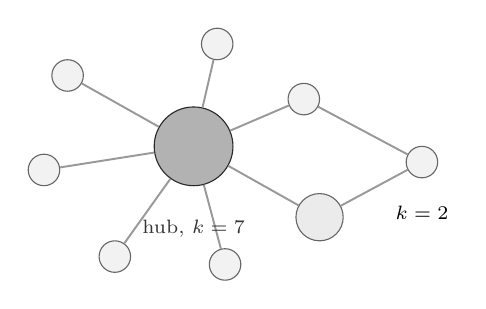
\begin{tikzpicture}[
  sm/.style={circle,draw=black!60,fill=black!5,minimum size=4mm,inner sep=0pt},
  md/.style={circle,draw=black!60,fill=black!8,minimum size=6mm,inner sep=0pt},
  hub/.style={circle,draw=accent!80!black,fill=black!30,minimum size=10mm,inner sep=0pt},
  lnk/.style={draw=black!40,line width=0.7pt}]
  \node[hub] (H) at (1.7,0.6) {};
  \node[sm] (n1) at (0.1,1.5)  {};
  \node[sm] (n2) at (-0.2,0.3) {};
  \node[sm] (n3) at (0.7,-0.8) {};
  \node[sm] (n4) at (2.0,1.9)  {};
  \node[sm] (n5) at (3.1,1.2)  {};
  \node[md] (n6) at (3.3,-0.3) {};
  \node[sm] (n7) at (2.1,-0.9) {};
  \node[sm] (m)  at (4.6,0.4)  {};
  \draw[lnk] (H)--(n1) (H)--(n2) (H)--(n3) (H)--(n4) (H)--(n5) (H)--(n6) (H)--(n7);
  \draw[lnk] (n6)--(m) (n5)--(m);
  \node[accent,font=\scriptsize] at (1.7,-0.45) {hub, $k=7$};
  \node[font=\scriptsize] at (4.6,-0.25) {$k=2$};
\end{tikzpicture}\end{adjustbox}
\caption{\textbf{Degree.} A node's degree is simply its number of links. Drawn
here with node size growing with degree: a few hubs (such as the central one,
$k=7$) carry many links, while most nodes have only one or two. That imbalance ---
many small nodes, a few giant hubs --- is the hallmark of a scale-free
network.}
\label{fig:intro-degree}
\end{figure}

\paragraph{Clustering coefficient.}
The \emph{clustering coefficient} measures cliquishness: of all the pairs of your
neighbors, what fraction are themselves connected? If you have four friends and
four of the possible six friendships among them actually exist, your clustering
coefficient is $4/6 \approx 0.67$. Formally, if node $i$ has $k_i$ neighbors and
$e_i$ of the possible links among those neighbors are present, then
\begin{equation}
  c_i = \frac{2 e_i}{k_i (k_i - 1)},
  \label{eq:intro-clustering}
\end{equation}
since $k_i(k_i-1)/2$ is the number of pairs that \emph{could} be linked. A
clustering coefficient near $1$ means a tight clique; near $0$ means your
contacts are strangers to each other. Averaged over all nodes we write $\langle
c\rangle$, where the angle brackets $\langle\cdot\rangle$ are standard shorthand
for ``average value.'' The striking empirical fact \citep{watts1998} is that
$\langle c\rangle$ in real networks is far larger than you would get by wiring
the same nodes up at random --- the quantitative fingerprint of those dense local
neighborhoods (Figure~\ref{fig:intro-clustering}).

\begin{figure}[t]
\centering
\begin{adjustbox}{max width=\linewidth}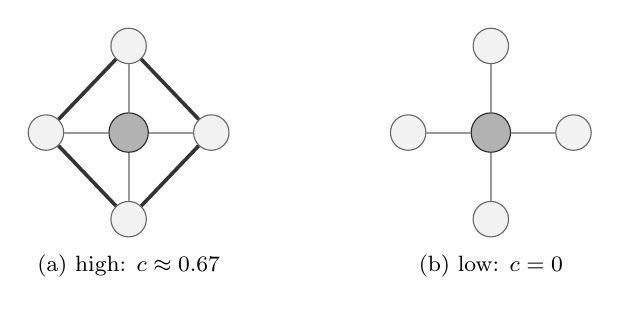
\begin{tikzpicture}[
  nd/.style={circle,draw=black!60,fill=black!5,minimum size=4.5mm,inner sep=0pt},
  ce/.style={circle,draw=accent!80!black,fill=black!30,minimum size=5mm,inner sep=0pt},
  lnk/.style={draw=black!40,line width=0.7pt},
  cl/.style={draw=accent,line width=1.3pt}]
  % (a) high clustering
  \begin{scope}
    \node[ce] (C) at (0,0)      {};
    \node[nd] (u1) at (0,1.1)   {};
    \node[nd] (u2) at (1.05,0)  {};
    \node[nd] (u3) at (0,-1.1)  {};
    \node[nd] (u4) at (-1.05,0) {};
    \draw[lnk] (C)--(u1) (C)--(u2) (C)--(u3) (C)--(u4);
    \draw[cl] (u1)--(u2) (u2)--(u3) (u3)--(u4) (u4)--(u1);
    \node[font=\footnotesize] at (0,-1.7) {(a) high: $c\approx0.67$};
  \end{scope}
  % (b) low clustering
  \begin{scope}[xshift=4.6cm]
    \node[ce] (D) at (0,0)      {};
    \node[nd] (v1) at (0,1.1)   {};
    \node[nd] (v2) at (1.05,0)  {};
    \node[nd] (v3) at (0,-1.1)  {};
    \node[nd] (v4) at (-1.05,0) {};
    \draw[lnk] (D)--(v1) (D)--(v2) (D)--(v3) (D)--(v4);
    \node[font=\footnotesize] at (0,-1.7) {(b) low: $c=0$};
  \end{scope}
\end{tikzpicture}\end{adjustbox}
\caption{\textbf{Clustering coefficient.} The clustering of the central node
(gray) is the fraction of its neighbor pairs that are themselves linked. (a) Four
of the six neighbor pairs are linked (the bold links), so $c\approx0.67$ --- a
cliquish neighborhood. (b) No neighbors are linked to each other, so
$c=0$.}
\label{fig:intro-clustering}
\end{figure}

\paragraph{Average distance.}
The \emph{distance} between two nodes is the number of links on the shortest
route between them --- the fewest hops to get from one to the other. Averaged
over all pairs of nodes, this distance grows very slowly (logarithmically, or
even more slowly) as the network gets bigger. Slow growth of distance, together
with high clustering, is precisely the small-world effect named above
(Figure~\ref{fig:intro-distance}).

\begin{figure}[t]
\centering
\begin{adjustbox}{max width=\linewidth}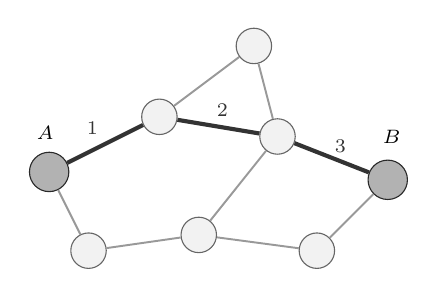
\begin{tikzpicture}[
  nd/.style={circle,draw=black!60,fill=black!5,minimum size=4.5mm,inner sep=0pt},
  ep/.style={circle,draw=accent!80!black,fill=black!30,minimum size=5mm,inner sep=0pt},
  lnk/.style={draw=black!40,line width=0.7pt},
  pth/.style={draw=accent,line width=1.5pt}]
  \node[ep] (A)  at (0,0)      {};
  \node[nd] (p1) at (1.4,0.7)  {};
  \node[nd] (p2) at (2.9,0.45) {};
  \node[ep] (B)  at (4.3,-0.1) {};
  \node[nd] (x1) at (0.5,-1.0) {};
  \node[nd] (x2) at (1.9,-0.8) {};
  \node[nd] (x3) at (3.4,-1.0) {};
  \node[nd] (x4) at (2.6,1.6)  {};
  \draw[lnk] (A)--(x1) (x1)--(x2) (x2)--(x3) (x3)--(B) (p1)--(x4) (p2)--(x4) (x2)--(p2);
  \draw[pth] (A)--(p1) (p1)--(p2) (p2)--(B);
  \node[accent,font=\scriptsize] at (0.55,0.55) {1};
  \node[accent,font=\scriptsize] at (2.2,0.78)  {2};
  \node[accent,font=\scriptsize] at (3.7,0.32)  {3};
  \node[font=\scriptsize] at (-0.05,0.5) {$A$};
  \node[font=\scriptsize] at (4.35,0.45) {$B$};
\end{tikzpicture}\end{adjustbox}
\caption{\textbf{Distance.} The distance between two nodes is the number of links
on the shortest route between them. The shortest route from $A$ to $B$ here is
three hops (in bold); the lower route is longer. In real networks these shortest
distances stay small even as the network grows --- the small-world
effect.}
\label{fig:intro-distance}
\end{figure}

\paragraph{Degree correlations.}
Now to the more subtle pattern. Imagine following a link from a node out to one
of its neighbors and asking: how connected is the neighbor I land on? If the
network had no \emph{degree correlations}, the answer would not depend on where I
started. But real networks are correlated: in some, high-degree hubs tend to sit
next to low-degree nodes; in others, hubs cluster together with other hubs. The
cleanest way to see this is to record, for nodes of each degree $k$, the
\emph{average degree of their neighbors}, written $\langle k_{nn}\rangle(k)$ (the
subscript ``nn'' stands for nearest-neighbors) \citep{pastorsatorras2001}:
\begin{equation}
  \langle k_{nn} \rangle(k) = \sum_{k'} k'\, p(k' \mid k).
  \label{eq:intro-knn}
\end{equation}
Here $p(k' \mid k)$ is read ``the probability that a link from a degree-$k$ node
lands on a degree-$k'$ node,'' and the sum simply averages the landing degree
$k'$ weighted by how likely each is. Do not worry if the formula looks abstract;
the next box pins down the one fact we need from it, and you can take that fact
on faith and skip the box if you prefer.

It is worth knowing what this quantity would be if there were \emph{no}
correlations at all, because that is the yardstick against which real networks
are judged.

\begin{calculation}{the no-correlation baseline for neighbor degree}
If degrees are uncorrelated, the only reason a link is more likely to land on a
particular node is that the node has more links to land on. The chance of
arriving at a node of degree $k'$ is then proportional to $k'$ times how common
such nodes are, $k' p(k')$. Averaging the landing degree $k'$ with this weight
(and dividing by the total weight to normalize) gives
\begin{equation}
  \langle k_{nn} \rangle_{\text{unc}}
  = \frac{\sum_{k'} k'\cdot k' p(k')}{\sum_{k'} k' p(k')}
  = \frac{\langle k^2 \rangle}{\langle k \rangle},
  \label{eq:intro-knn-unc}
\end{equation}
where $\langle k\rangle$ is the average degree and $\langle k^2\rangle$ the
average of the squared degree.
\end{calculation}

The result, Eq.~\eqref{eq:intro-knn-unc}, is the key takeaway: in a network with
no degree correlations, the average neighbor degree is the same flat number for
every node, regardless of that node's own degree. So when we plot $\langle
k_{nn}\rangle(k)$ against $k$ for a real network and the curve is \emph{not}
flat, the tilt tells us the kind of correlation present. If the curve slopes
\emph{down} --- well-connected nodes have poorly-connected neighbors --- the
network is called \emph{disassortative}; this is typical of technological and
biological networks. If it slopes \emph{up} --- the well-connected keep company
with the well-connected --- the network is \emph{assortative}, as social networks
tend to be \citep{newman2002}. Assortative and disassortative are simply the
``birds of a feather'' and ``opposites attract'' of network connectivity
(Figure~\ref{fig:intro-correlations}).

\begin{figure}[t]
\centering
\begin{adjustbox}{max width=\linewidth}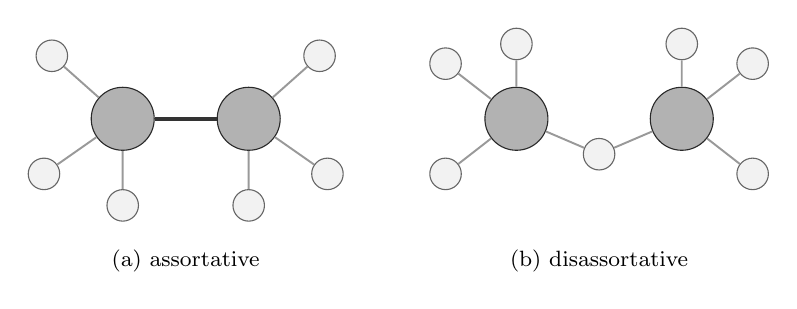
\begin{tikzpicture}[
  nd/.style={circle,draw=black!60,fill=black!5,minimum size=4mm,inner sep=0pt},
  hub/.style={circle,draw=accent!80!black,fill=black!30,minimum size=8mm,inner sep=0pt},
  lnk/.style={draw=black!40,line width=0.7pt},
  hl/.style={draw=accent,line width=1.3pt}]
  % (a) assortative: hubs link to hubs
  \begin{scope}
    \node[hub] (Ha) at (0.7,0.3) {};
    \node[hub] (Hb) at (2.3,0.3) {};
    \draw[hl] (Ha)--(Hb);
    \node[nd] (a1) at (-0.2,1.1) {}; \node[nd] (a2) at (-0.3,-0.4) {}; \node[nd] (a3) at (0.7,-0.8) {};
    \node[nd] (b1) at (3.2,1.1)  {}; \node[nd] (b2) at (3.3,-0.4)  {}; \node[nd] (b3) at (2.3,-0.8) {};
    \draw[lnk] (Ha)--(a1) (Ha)--(a2) (Ha)--(a3) (Hb)--(b1) (Hb)--(b2) (Hb)--(b3);
    \node[font=\footnotesize] at (1.5,-1.5) {(a) assortative};
  \end{scope}
  % (b) disassortative: hubs link to low-degree nodes
  \begin{scope}[xshift=5.2cm]
    \node[hub] (Hc) at (0.5,0.3)  {};
    \node[hub] (Hd) at (2.6,0.3)  {};
    \node[nd] (mid) at (1.55,-0.15) {};
    \draw[lnk] (Hc)--(mid) (Hd)--(mid);
    \node[nd] (c1) at (-0.4,1.0) {}; \node[nd] (c2) at (-0.4,-0.4) {}; \node[nd] (c3) at (0.5,1.25) {};
    \node[nd] (d1) at (3.5,1.0)  {}; \node[nd] (d2) at (3.5,-0.4)  {}; \node[nd] (d3) at (2.6,1.25) {};
    \draw[lnk] (Hc)--(c1) (Hc)--(c2) (Hc)--(c3) (Hd)--(d1) (Hd)--(d2) (Hd)--(d3);
    \node[font=\footnotesize] at (1.55,-1.5) {(b) disassortative};
  \end{scope}
\end{tikzpicture}\end{adjustbox}
\caption{\textbf{Degree correlations.} (a) In an \emph{assortative} network, hubs
tend to link to other hubs (``birds of a feather''). (b) In a
\emph{disassortative} one, hubs avoid each other and link instead to low-degree
nodes (``opposites attract''). Social networks lean assortative; technological and
biological ones, disassortative.}
\label{fig:intro-correlations}
\end{figure}

\paragraph{Clustering hierarchy.}
Finally, we can combine the last two ideas by asking how cliquishness depends on
degree. Sorting nodes by their degree $k$ and averaging the clustering
coefficient within each group gives $\langle c\rangle(k)$. In a wide range of
real networks this quantity falls off as a power law,
\begin{equation}
  \langle c \rangle(k) \sim k^{-1},
  \label{eq:intro-hierarchy}
\end{equation}
meaning the more connections a node has, the \emph{less} cliquish its
neighborhood. This is the \emph{clustering hierarchy}, and it has an intuitive
reading \citep{ravasz2002,ravasz2003}: ordinary low-degree nodes sit inside
tight little communities where everyone knows everyone, while the big hubs act as
bridges between many such communities, so their own neighbors --- drawn from all
over --- mostly do not know each other. A small-town local has a dense circle of
mutual friends; a globe-trotting connector knows thousands of people who have
never met (Figure~\ref{fig:intro-hierarchy}).

\begin{figure}[t]
\centering
\begin{adjustbox}{max width=\linewidth}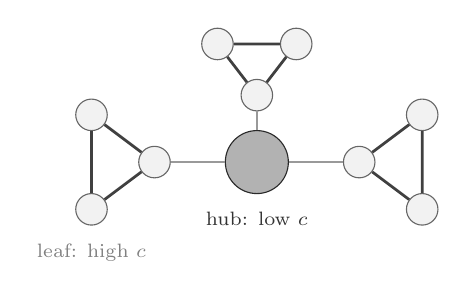
\begin{tikzpicture}[
  nd/.style={circle,draw=black!60,fill=black!5,minimum size=4mm,inner sep=0pt},
  hub/.style={circle,draw=accent!80!black,fill=black!30,minimum size=8mm,inner sep=0pt},
  lnk/.style={draw=black!40,line width=0.7pt},
  tri/.style={draw=black!75,line width=1.0pt}]
  \node[hub] (H) at (2.0,0) {};
  % left cluster
  \node[nd] (l1) at (-0.1,0.6) {}; \node[nd] (l2) at (-0.1,-0.6) {}; \node[nd] (l3) at (0.7,0) {};
  \draw[tri] (l1)--(l2) (l2)--(l3) (l3)--(l1);  \draw[lnk] (l3)--(H);
  % top cluster
  \node[nd] (t1) at (1.5,1.5) {}; \node[nd] (t2) at (2.5,1.5) {}; \node[nd] (t3) at (2.0,0.85) {};
  \draw[tri] (t1)--(t2) (t2)--(t3) (t3)--(t1);  \draw[lnk] (t3)--(H);
  % right cluster
  \node[nd] (r1) at (4.1,0.6) {}; \node[nd] (r2) at (4.1,-0.6) {}; \node[nd] (r3) at (3.3,0) {};
  \draw[tri] (r1)--(r2) (r2)--(r3) (r3)--(r1);  \draw[lnk] (r3)--(H);
  \node[accent,font=\scriptsize]  at (2.0,-0.72) {hub: low $c$};
  \node[accentB,font=\scriptsize] at (-0.1,-1.15) {leaf: high $c$};
\end{tikzpicture}\end{adjustbox}
\caption{\textbf{Clustering hierarchy.} Low-degree nodes sit inside tight clusters
where everyone is connected (high clustering, the dark triangles), while a hub
bridges many such clusters. The hub's own neighbors --- one drawn from each
cluster --- do not know each other, so the hub itself has low clustering.
Cliquishness therefore falls as degree rises.}
\label{fig:intro-hierarchy}
\end{figure}

A word of caution ties the last two measures together, for they are not as
independent as they look. The clustering hierarchy and the degree correlations
are, in part, two views of the same thing. To see why, take a hub in a
disassortative network: its neighbors are mostly low-degree nodes, and a
low-degree node has too few links to be connected to many of the hub's other
neighbors. The hub is therefore \emph{forced} to have low clustering, not
because of any designed hierarchy but simply because of whom it is attached to.
Some of the observed decay of $\langle c\rangle(k)$ with degree is thus an
automatic by-product of the degree correlations, not independent evidence of
modular organization. Indeed, when one strips out this bias and measures the
clustering that remains, it is often roughly constant, or decays only very
weakly, with degree \citep{soffer2005}. The lesson is to read these measures
together rather than in isolation --- a theme that recurs throughout the book,
where a single local rule will be seen to set the clustering hierarchy and the
degree correlations \emph{at once}, as facets of one mechanism.

\section{From global to local rules}

With the measures in hand we can state the puzzle this book exists to solve. The
modern story of network growth opens with the model of \citet{barabasi1999},
usually abbreviated BA after its authors. It rests on two ideas. The first is
\emph{growth}: networks are not built all at once but accumulate nodes over time,
the way the Web gains pages or the literature gains papers. The second is
\emph{preferential attachment}: a new node prefers to link to nodes that are
already well connected, with a probability proportional to their degree --- the
``rich get richer'' of networks. From these two ingredients a power-law degree
distribution follows reliably, and preferential attachment has rightly become the
textbook explanation for why so many networks are scale-free.

Two difficulties, though, drive everything that follows. The first is about
\emph{mechanism}. Preferential attachment, read literally, is a \emph{global}
rule: to attach in proportion to degree, a newcomer would have to know the degree
of every node in the entire network and weigh them all against each other.
That is implausible for the systems we care about. A scientist writing a new
paper has read a few dozen others, not the millions in existence; a new gene is a
copy of one existing gene, ignorant of the rest of the genome; a newcomer to a
town meets a handful of people, not the whole population. Real nodes act
\emph{locally}. So if preferential attachment is not literally true, why do so
many networks behave as if it were?

The second difficulty is that the BA model, for all its success with the degree
distribution, does not by itself reproduce the other patterns we just met. Its
clustering fades away as the network grows, it shows none of the clustering
hierarchy of Eq.~\eqref{eq:intro-hierarchy}, and its degree correlations are weak
\citep{albert2002,vazquez2003}. Something is missing.

The resolution pursued throughout this book is to throw out the global rule and
replace it with local ones, then watch what \emph{emerges}. By a \emph{local
rule} we mean a way of growing the network in which a newcomer reaches some node
--- chosen at random, or arrived at by surfing along links, or copied from an
existing node --- and then connects to that node and perhaps to a few of its
immediate neighbors, using nothing but that local information. The recurring and
rather beautiful discovery, established for several such rules
\citep{vazquez2003}, is that
\begin{quote}
\emph{an effective ``rich get richer'' behavior arises all on its own from
growth by local rules.}
\end{quote}
The reason, which we will meet many times, is almost a slogan: a well-connected
node is, by definition, a node that many local explorations will bump into,
because it has many links through which it can be reached. The preference for
hubs need not be legislated; it is a free by-product of poking around the network
locally. And because the very same local moves also create triangles (your
friend introduces you to their friend) and link nodes of unlike degree, the same
rules that produce the power law deliver, in one package, the clustering
hierarchy of Eq.~\eqref{eq:intro-hierarchy} and the degree correlations of
Eq.~\eqref{eq:intro-knn}. Three patterns that look independent turn out to share
a single root.

\section{What the data demand}

Any explanation has to answer to measurements, so it is worth recording up front
what those measurements actually look like. Rather than take this on trust, let us
measure four real networks and see. All four come from the Netzschleuder
repository \citep{netzschleuder}, a public catalogue of several hundred network
datasets, read here through the \texttt{graph-tool} library \citep{peixoto2014};
the code that fetches and measures them accompanies this book. They are: the
\emph{Internet} at the level of the service providers, the ``autonomous
systems,'' that own its routers; the \emph{Gnutella} peer-to-peer file-sharing
overlay; the protein interaction network of \emph{yeast}; and the
\emph{co-authorship} network of the \texttt{cond-mat} preprint archive, in which
two physicists are linked if they have written a paper together. Three
technological or biological, one social --- which turns out to be exactly the
division that matters.

Start with the small world, since it needs only two numbers per network
(Table~\ref{tab:intro-data}). Every one of these networks is small: the average
distance between two nodes is between four and seven hops, in networks of up to
sixty thousand nodes. And every one is far more cliquish than chance. Wiring the
same number of nodes at random with the same number of links --- the comparison
Watts and Strogatz made --- would give the clustering in the column headed
$\langle c\rangle_{\mathrm{ER}}$, which is between forty and two and a half
thousand times smaller than what is observed. The comparison is almost unfair,
though, because it also throws away the hubs, and hubs alone create some
clustering. The last of the clustering columns is therefore the honest one: it
shuffles the links at random while holding every node's degree fixed, and measures
what survives. Even against that stricter null the real networks are the more
cliquish, by factors of two to three hundred. The cliquishness is real, and it is
not merely a shadow of the degree distribution.

\begin{table}[t]
\centering
\footnotesize
\setlength{\tabcolsep}{3.2pt}
\caption{\textbf{Four real networks.} Measured on the largest connected component,
undirected. $\langle c\rangle_{\mathrm{ER}}$ is the clustering of a random network
with the same $n$ and $\langle k\rangle$; $\langle c\rangle_{\mathrm{rew}}$ that
of the same network with its links shuffled at random but every degree held fixed.
$\langle d\rangle$ is the average distance and $r$ the assortativity: negative for
the first three, positive for the last.}
\label{tab:intro-data}
\begin{tabular}{lrrrrrrr}
\hline
Network & $n$ & $\langle k\rangle$ & $\langle c\rangle$ &
$\langle c\rangle_{\mathrm{ER}}$ & $\langle c\rangle_{\mathrm{rew}}$ &
$\langle d\rangle$ & $r$ \\
\hline
Internet (AS)  & $22\,963$ & $4.2$ & $0.230$ & $0.0002$ & $0.125$  & $3.9$ & $-0.052$ \\
Gnutella       & $62\,561$ & $4.7$ & $0.005$ & $0.0001$ & $0.0002$ & $5.9$ & $-0.036$ \\
Yeast proteins & $1\,458$  & $2.7$ & $0.071$ & $0.0018$ & $0.0026$ & $6.9$ & $-0.034$ \\
cond-mat       & $36\,458$ & $9.4$ & $0.657$ & $0.0003$ & $0.0020$ & $5.5$ & $+0.055$ \\
\hline
\end{tabular}
\end{table}

Now the three measures that organize the rest of the book
(Figure~\ref{fig:intro-data}). The degree distributions are broad and
hub-dominated: the Internet runs from nodes with a single link to one with more
than two thousand, four decades of degree in a network four decades in size, and
the others do the same over a shorter range. Gnutella is the partial exception
worth naming --- its protocol caps how many peers a client will hold, so its tail
is cut short and it is the least scale-free of the four. Real data are like that;
the power law of Eq.~\eqref{eq:intro-powerlaw} is an idealization that some
systems wear better than others.

The clustering hierarchy of Eq.~\eqref{eq:intro-hierarchy} is there in all four:
$\langle c\rangle(k)$ falls with degree in every case, and the dashed $k^{-1}$
guide shows that the decay is of about the advertised steepness --- the measured
slopes run from $-0.6$ to $-1.3$. Small nodes sit in tight neighborhoods; hubs
bridge between them.

And then the two families part company, on the last measure and only on the last
measure. For the Internet, for Gnutella and for the yeast proteins, the average
neighbor degree \emph{falls} with degree: these networks are
\emph{disassortative}, their hubs presiding over peripheries of poorly-connected
nodes rather than huddling together. This is the signature of technological and
biological networks \citep{pastorsatorras2001,maslov2002,jeong2001}. For the
co-authorship network it \emph{rises}: prolific, well-connected authors tend to
write with one another, and the network is \emph{assortative}
\citep{newman2002}. The single number $r$ in Table~\ref{tab:intro-data} says the
same thing more briefly --- negative for the first three, positive for the fourth
--- and the sign of that number is the cleanest division in the data.

The contrast between the two families is instructive, because it shows that
whatever mechanism we propose must be able to produce \emph{either} sign of
correlation, depending on the microscopic move --- and, as the chapters will show,
local rules can do exactly that. It also tells us the two families are not two
kinds of network but one kind seen through one dial: everything else in
Figure~\ref{fig:intro-data} they share.

\begin{figure}[t]
\centering
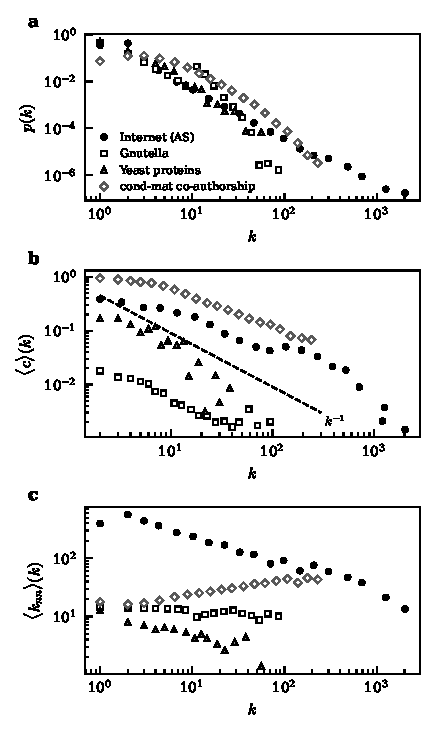
\includegraphics[width=\linewidth]{figs/fig-intro-data.pdf}
\caption{\textbf{What the data demand.} Four real networks from the Netzschleuder
repository, measured through \texttt{graph-tool}. (a) The degree distributions are
broad and hub-dominated; the Internet spans four decades of degree. Gnutella's
protocol caps its peers, so its tail is the shortest. (b) The clustering hierarchy
of Eq.~\eqref{eq:intro-hierarchy}: $\langle c\rangle(k)$ falls with degree in every
network, at roughly the advertised $k^{-1}$ (dashed guide). (c) The average
neighbor degree, where the two families part: falling for the Internet, Gnutella
and the yeast proteins --- \emph{disassortative} --- but rising for cond-mat
co-authorship, which is \emph{assortative}.}
\label{fig:intro-data}
\end{figure}

These regularities are robust, they hold across many orders of magnitude in
network size, and for years their shared origin was a mystery. Supplying that
origin, one mechanism and one class of networks at a time, is the work of this
book.

\section{Plan of the book}

The chapters proceed from mechanism to application, each built around one
concrete local rule and a family of real networks it illuminates. The reader
need not take any chapter on faith: in each, a simple local rule is stated, its
consequences are worked out (with the heavier algebra confined to boxes that can
be skipped), and the predictions are held up against real data.

\begin{itemize}
  \item \textbf{Search and connect.} A newcomer learns of existing nodes by
    exploring the network --- following references, surfing hyperlinks,
    performing a random walk --- and connects to what it finds. This is the
    natural model for searchable, directed networks such as the citation network
    and the World Wide Web, and it is where we show in detail how the simple act
    of surfing manufactures an effective ``rich get richer.''

  \item \textbf{Friends of friends.} A newcomer connects to a node and then to
    some of that node's neighbors --- you meet a person, then their friends. This
    rule for social network growth creates triangles directly, and it generates
    the assortative correlations and the cliquishness hierarchy of social
    networks.

  \item \textbf{Gene duplication.} Biological networks grow by copying: a node is
    duplicated together with its connections, after which links are gained and
    lost. Duplication is an intrinsically local move, and it explains the
    disassortative, hierarchical structure of protein interaction networks.

  \item \textbf{Activity specialization.} The schedule of a large project is a
    network of activities grown by a local refinement rule: each activity is
    either duplicated into parallel copies or split into specialized sequential
    parts. The same copying mechanism gives power-law degrees, while making the
    celebrated ``critical path'' vanish as projects grow and relocating delay
    risk in the network as a whole.

  \item \textbf{Emergence of communities.} Local rules do not only set degrees
    and correlations; they also organize nodes into communities --- tight groups
    with many links inside and few outside. We examine how this mesoscale
    structure arises from the same local dynamics, even when every node is
    otherwise identical.

  \item \textbf{Boosting shortest path multiplicity.} Finally we turn to the
    redundancy of routes through a network --- how many equally short paths join
    two nodes --- and show that local growth multiplies them, tying this
    redundancy to the very community structure of the previous chapter.
\end{itemize}

A single thread runs through all of them. In each case the apparently global
features of a network --- its scale-free degrees, its small-world distances, its
clustering hierarchy, its degree correlations, its communities, its redundant
paths --- turn out to be the collective, emergent consequence of simple rules that
no node applies with more than local knowledge. That is the sense in which the
title of this book should be read: not networks built by a designer, but networks
that grow themselves, one local decision at a time.


% instructions
% references
% - https://www.researchgate.net/publication/395472157_Degree_correlations_and_clustering_hierarchy_in_networks_measures_origin_and_consequences, chapter 2
% - https://arxiv.org/abs/cond-mat/0211528, section I


\chapter{Search and connect}
\label{ch:search}

\section{Finding what to link to}

The introduction left us with a puzzle. The ``rich get richer'' rule explains
why so many networks are scale-free, but as a literal recipe it asks the
impossible: a newcomer would have to know the degree of every node in the
network in order to favor the well-connected ones. In this chapter we solve the
puzzle for an important family of networks --- the \emph{searchable} ones --- by
replacing that impossible global rule with the most natural local act a newcomer
can perform. It \emph{searches} the network, moving from node to node along the
links, and connects to what it happens to find.

The systems to keep in mind are collections of documents that point at one
another. In the \emph{citation network}, each node is a published article and
each link is a reference from one article to another. In the World Wide Web,
each node is a page and each link is a hyperlink. These are \emph{directed}
networks: a reference, like a hyperlink, points one way. An article cites an
older one, not the reverse; a page links to another, which need not link back.
Because direction matters, each node now has two kinds of degree. Its
\emph{in-degree}, written $k^{in}$, counts the links pointing \emph{at} it ---
how many times a paper has been cited, how many pages link to a given page. Its
\emph{out-degree}, written $k^{out}$, counts the links pointing \emph{out} of it
--- how many references a paper makes, how many hyperlinks a page contains. It is
the in-degree that interests us, because in real document networks it is the
in-degree --- the count of incoming attention --- that is broadly distributed,
with a few hugely-cited classics and a long tail of papers cited once or never.

How does a new document come to point at the old ones? Not by consulting a
global popularity ranking. An author writing a new paper finds references by
reading a few papers and following \emph{their} reference lists, and then the
references of those, and so on \citep{price1965}. A web author discovers pages by
surfing from link to link and by typing queries into a search engine
\citep{brin1998}. In every case the information used is strictly local --- a
document one has reached, and the documents it points to. The claim of this
chapter is that this local searching, repeated by every newcomer, adds up to
exactly the ``rich get richer'' behavior that the introduction had to assume by
fiat, and that it brings the power-law degrees, the clustering hierarchy, and
the degree correlations along with it \citep{vazquez2001,vazquez2003}.

\section{Surfing as a random walk}

To turn ``surfing'' into something we can analyze, we model the surfer as a
\emph{random walker} on the network. A random walk is just what it sounds like:
start somewhere, and step to a randomly chosen neighbor, then to a neighbor of
\emph{that} node, and so on. Our surfer does this with a twist. From whatever
page it is on, with probability $q_e$ it follows one of that page's outgoing
hyperlinks, picked at random; with the remaining probability $1-q_e$ it gets
bored, stops following links, and jumps to a completely random page elsewhere.
The single dial $q_e$, a number between $0$ and $1$, sets how patiently the
surfer explores along links before restarting from scratch.

Now ask: in the long run, what fraction of its time does the walker spend at
each page? Call that fraction the page's \emph{visiting probability}, $v_i$ for
node $i$. A page is visited often if many links point to it and those linking
pages are themselves visited often --- a self-referential condition that turns
out to have a clean form. The remarkable thing, worth flagging before any
algebra, is that this visiting probability is \emph{exactly the quantity that
Google was built on}: it is the \emph{PageRank} of the page, the measure of
importance that ranks search results \citep{brin1998}. So the local rule we are
about to write is not a toy --- it is the very process real search engines compute
and then display to the authors who go on to create new links.

\begin{figure}[t]
\centering
\begin{adjustbox}{max width=\linewidth}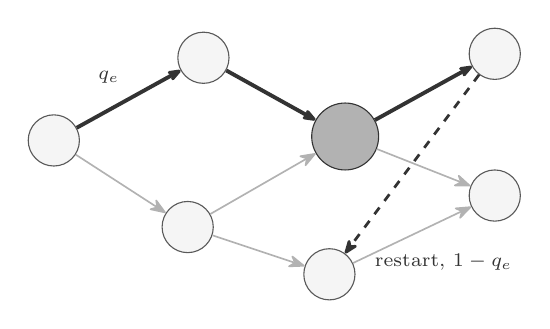
\begin{tikzpicture}[>={Stealth[round,length=2.4mm]},
  nd/.style={circle,draw=black!65,fill=black!4,minimum size=6.5mm,inner sep=0pt},
  hub/.style={circle,draw=accent,fill=black!30,minimum size=8.5mm,inner sep=0pt},
  ex/.style={->,draw=black!30,line width=0.6pt},
  walk/.style={->,draw=accent,line width=1.4pt},
  jump/.style={->,draw=accent,line width=1.0pt,dashed}]
  \node[nd]  (n1) at (0,0)      {};
  \node[nd]  (n2) at (1.9,1.05) {};
  \node[nd]  (n3) at (1.7,-1.1) {};
  \node[hub] (n4) at (3.7,0.05) {};
  \node[nd]  (n5) at (3.5,-1.7) {};
  \node[nd]  (n6) at (5.6,1.1)  {};
  \node[nd]  (n7) at (5.6,-0.7) {};
  \draw[ex] (n1) -- (n3);
  \draw[ex] (n3) -- (n4);
  \draw[ex] (n3) -- (n5);
  \draw[ex] (n4) -- (n7);
  \draw[ex] (n5) -- (n7);
  \draw[walk] (n1) -- (n2);
  \draw[walk] (n2) -- (n4);
  \draw[walk] (n4) -- (n6);
  \draw[jump] (n6) -- (n5);
  \node[accent,font=\scriptsize] at (0.7,0.8)  {$q_e$};
  \node[accent,font=\scriptsize] at (4.95,-1.55) {restart, $1-q_e$};
\end{tikzpicture}\end{adjustbox}
\caption{\textbf{Surfing as a random walk.} From the page it is on, the searcher
follows one of the outgoing links with probability $q_e$ (solid arrows) or, with
probability $1-q_e$, jumps to a page chosen at random (dashed arrow). A page
reached along many routes --- like the highlighted hub --- is visited most often;
this visiting frequency is the page's PageRank, and it grows in proportion to the
number of links that point at the page.}
\label{fig:walk-surf}
\end{figure}

The picture to keep in mind is Figure~\ref{fig:walk-surf}. We would like to know
how a page's visiting probability depends on its
in-degree. Getting there exactly is hard, so we make the standard physicist's
move of replacing fluctuating quantities by their averages --- a so-called
\emph{mean-field approximation}, ``mean'' as in average. The next box carries
this out; the one sentence to carry away is stated right after it, so the box
can be skipped.

\begin{calculation}{from surfing to the visiting probability}
The visiting probability of node $i$ obeys a balance condition: the walker
arrives at $i$ either by a random jump (probability $1-q_e$, landing on any of
the $n$ nodes equally) or by following a link into $i$ from some node $j$ that
points to it,
\begin{equation}
  v_i = \frac{1-q_e}{n} + q_e \sum_j a_{ij}\, \frac{v_j}{k^{out}_j},
  \label{eq:walk-pagerank}
\end{equation}
where $a_{ij}=1$ when $j$ points to $i$, and the factor $1/k^{out}_j$ accounts
for $j$ spreading its attention over its $k^{out}_j$ outgoing links. This is the
PageRank equation. To simplify it, replace the sum over the specific nodes
pointing to $i$ by an average. A node is reached along an incoming link from a
node of out-degree $k^{out}$ with probability $k^{out} p_{k^{out}}/\langle
k^{out}\rangle$, and that link is then followed with probability $1/k^{out}$; the
two factors of $k^{out}$ cancel, so each incoming link contributes the same
average amount $\Theta = \langle v\rangle/\langle k^{out}\rangle$. Since node $i$
has $k^{in}_i$ incoming links,
\begin{equation}
  v_i = \frac{1-q_e}{n} + q_e\, \Theta\, k^{in}_i.
  \label{eq:walk-vi-mf}
\end{equation}
\end{calculation}

The payoff is Eq.~\eqref{eq:walk-vi-mf}, and it is simple to state in words: a
page's visiting probability grows in a straight line with its in-degree. Double
the number of links pointing at a page and you roughly double how often the
surfer lands on it. That straight-line relationship is the seed from which
everything in this chapter grows.

\section{An effective ``rich get richer''}

Being visited is not the same as being linked to --- you read many pages you do
not cite. So suppose that each time the surfer visits a page it creates a new
incoming link to it only with some probability $q_v$. We can then ask how fast a
page accumulates new links as a function of how many it already has. This rate
is the network-growth analog of preferential attachment, and computing it is the
crux of the chapter. The derivation is short; its conclusion is in the sentence
after the box.

\begin{calculation}{the rate at which a page gains links}
Let $\nu_s$ surfers be active and $\nu_a$ new pages be added per unit time. The
node count $n$ and link count $e$ grow as
\begin{equation}
  \frac{\partial n}{\partial t} = \nu_a, \qquad
  \frac{\partial e}{\partial t} = \nu_s\, q_v\, \langle v \rangle\, n,
  \label{eq:walk-growth}
\end{equation}
because each of the $\langle v\rangle n$ visits in a walk makes a link with
probability $q_v$. Integrating fixes the average degree and hence $\Theta =
\nu_a/(q_v\nu_s n)$. The rate at which a page of in-degree $k^{in}$ gains its
next link is $A(k^{in}) = q_v\, v(k^{in})$; substituting
Eq.~\eqref{eq:walk-vi-mf} and the value of $\Theta$,
\begin{equation}
  A(k^{in}) = \frac{1}{n}\left[\, q_v(1-q_e) + q_e\, \frac{\nu_a}{\nu_s}\, k^{in} \right].
  \label{eq:walk-attach}
\end{equation}
\end{calculation}

Equation~\eqref{eq:walk-attach} is the central result, and it deserves to be
read slowly. The rate at which a page attracts new links has two parts: a
constant piece, the same for every page, which gives even a brand-new page a
chance of being noticed; and a piece \emph{proportional to its current
in-degree}. That second piece is preferential attachment --- the rich getting
richer --- but notice where it came from. The surfer never consulted a global
ranking of pages; it only followed links, one at a time. The bias toward
well-connected pages appeared on its own, for the simple reason that a page with
many incoming links is a page the wandering surfer reaches by many routes. We
have \emph{derived} the rule the introduction had to assume. The same logic
underlies the ``redirection'' trick of \citet{krapivsky2001}, in which a newcomer
points either to a random node or to whatever that node points to --- a one-step
walk that yields the same effective preference.

\section{The degree distribution}

A linear attachment rate is exactly the ingredient needed to produce a power
law. Working out the resulting distribution of in-degrees requires solving a
balance equation for how many pages sit at each in-degree, which we do in the
box. Readers willing to take the outcome on trust can jump to the discussion
after it.

\begin{calculation}{the in-degree distribution and its exponent}
Let $n_{k^{in}}$ be the number of nodes with in-degree $k^{in}$. It changes as
nodes climb from one in-degree to the next by gaining links, with new nodes
injected at in-degree zero:
\begin{equation}
  \frac{\partial n_{k^{in}}}{\partial t}
  = \nu_s\, A_{k^{in}-1}\, n_{k^{in}-1}
  - \nu_s\, A_{k^{in}}\, n_{k^{in}}
  + \nu_a\, \delta_{k^{in},0}\,,
  \label{eq:walk-rate}
\end{equation}
the symbol $\delta_{k^{in},0}$ being $1$ only at $k^{in}=0$. For a network
growing at a constant rate the ratio $\nu_s/\nu_a=\alpha$ is fixed and the shape
of the distribution settles down, $n_{k^{in}}(t)=N p_{k^{in}}$. Solving for that
stationary shape gives (with $\Gamma$ the gamma function, a smooth
generalization of the factorial)
\begin{equation}
  p_{k^{in}} = \frac{1}{1+a}\,
  \frac{\Gamma[a(\gamma-1)+k^{in}]}{\Gamma[a(\gamma-1)]}\;
  \frac{\Gamma[(1+a)(\gamma-1)+1]}{\Gamma[(1+a)(\gamma-1)+k^{in}+1]},
  \label{eq:walk-pk}
\end{equation}
\begin{equation}
  \gamma = 1 + \frac{1}{q_e}, \qquad a = \alpha\, q_v\,(1-q_e),
  \label{eq:walk-gamma}
\end{equation}
which for large in-degree is the power law
\begin{equation}
  p_{k^{in}} \sim (k^{in})^{-\gamma}.
  \label{eq:walk-asym}
\end{equation}
\end{calculation}

Two features of the result, Eq.~\eqref{eq:walk-gamma}, are worth dwelling on.
First, the exponent $\gamma$ is at least $2$ --- exactly the range seen in real
citation and web networks. Second, and more surprising, $\gamma$ depends
\emph{only} on $q_e$, the surfer's patience for following links. It does not
depend on $q_v$, how often readers actually cite what they read, nor on the
growth rate of the network. Whether authors are generous or stingy with
citations changes how many links there are, but not the \emph{shape} of the
distribution; only the manner of \emph{exploring} the network does that. As the
surfer explores ever more deeply ($q_e\to 1$) the exponent drops to its minimum
of $2$, the most hub-dominated case; as the surfer restarts constantly ($q_e\to
0$) the exponent grows without bound and the heavy tail of hubs disappears.

\section{Cliquishness and correlations}

The same walk that sets the degrees also lays down triangles, so it predicts the
clustering hierarchy of the introduction with no extra assumptions. The reason
is simple to picture: whenever the surfer steps from a page to one of that
page's neighbors and links to both, it has closed a triangle. A short
calculation turns this picture into a formula.

\begin{calculation}{how clustering falls with degree}

Counting the links $e_i$ among the neighbors of node $i$ created by the walk 
gives $\partial e_i/\partial t \approx (1+q_e)\,\partial k^{in}_i/\partial 
t$. Integrating this differential equation, assuming $e = 0$ for $k = 1$, we 
obtain $e = (1 + q_e) (k - 1)$. Inserting this into the definition of the 
clustering coefficient,
$\langle c\rangle_k = 2e(k)/[k(k-1)]$, yields
\begin{equation}
  \langle c \rangle_k \approx \frac{2(1+q_e)}{k}.
  \label{eq:walk-ck}
\end{equation}
\end{calculation}

The message of Eq.~\eqref{eq:walk-ck} is that cliquishness is inversely
proportional to degree: a node with twice the degree has roughly half the
clustering. This is precisely the clustering hierarchy of
Eq.~\eqref{eq:intro-hierarchy}, seen in the Internet, the Web, and the protein
network --- and here it falls out for free from growth by searching. The
intuition is that a node gains a triangle every time the surfer steps from it to
a neighbor, so its triangles grow in step with its degree, while the number of
\emph{possible} triangles grows much faster, like the square of the degree;
their ratio, the clustering, therefore falls off as one over the degree.

The degree correlations are governed by the same single dial $q_e$. Numerical
simulation of the model shows that when $q_e$ is small the network looks
essentially uncorrelated --- the average neighbor degree is flat, as in the
baseline of Eq.~\eqref{eq:intro-knn-unc} --- while as $q_e$ grows the average
neighbor degree develops the downward slope of a \emph{disassortative} network,
hubs sitting amid poorly-connected pages. This matches the real Web, whose
measured exponent $\gamma\approx 2.1$ corresponds through
Eq.~\eqref{eq:walk-gamma} to a patient surfer with $q_e>0.5$, squarely in the
disassortative regime. One knob, $q_e$, thus fixes the degree-distribution
exponent, the cliquishness hierarchy, and the sign of the correlations all at
once --- tying together what the introduction presented as three separate facts.

\section{Two ways to search}

It helps to see two concrete versions of the searching rule, because they behave
differently and bracket the range of possibilities. Figure~\ref{fig:walk-models}
contrasts them.

\begin{figure}[t]
\centering
\begin{adjustbox}{max width=\linewidth}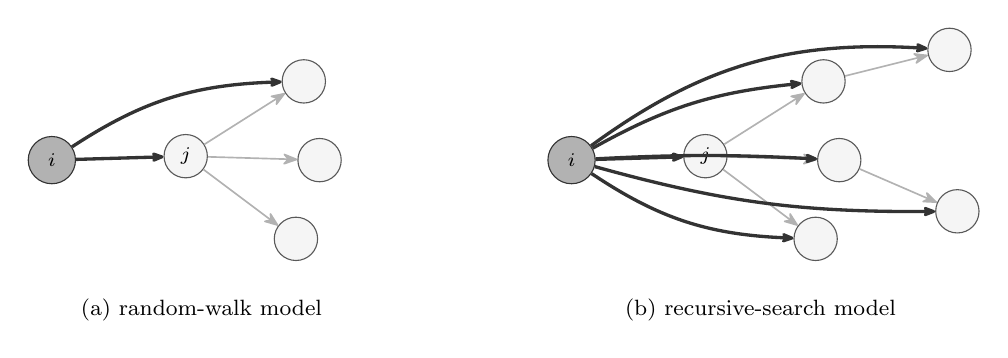
\begin{tikzpicture}[>={Stealth[round,length=2.2mm]},
  nd/.style={circle,draw=black!65,fill=black!4,minimum size=5.5mm,inner sep=0pt,font=\scriptsize},
  new/.style={circle,draw=accent,fill=black!30,minimum size=6mm,inner sep=0pt,font=\scriptsize},
  ex/.style={->,draw=black!30,line width=0.6pt},
  add/.style={->,draw=accent,line width=1.2pt}]
  % panel (a): random-walk model
  \begin{scope}
    \node[nd]  (j)  at (0,0)       {$j$};
    \node[nd]  (m1) at (1.5,0.95)  {};
    \node[nd]  (m2) at (1.7,-0.05) {};
    \node[nd]  (m3) at (1.4,-1.05) {};
    \draw[ex] (j)--(m1); \draw[ex] (j)--(m2); \draw[ex] (j)--(m3);
    \node[new] (i) at (-1.7,-0.05) {$i$};
    \draw[add] (i)--(j);
    \draw[add] (i) to[bend left=16] (m1);
    \node[font=\footnotesize] at (0.2,-1.95) {(a) random-walk model};
  \end{scope}
  % panel (b): recursive-search model
  \begin{scope}[xshift=6.6cm]
    \node[nd]  (jj) at (0,0)       {$j$};
    \node[nd]  (q1) at (1.5,0.95)  {};
    \node[nd]  (q2) at (1.7,-0.05) {};
    \node[nd]  (q3) at (1.4,-1.05) {};
    \node[nd]  (p1) at (3.1,1.35)  {};
    \node[nd]  (p2) at (3.2,-0.7)  {};
    \draw[ex] (jj)--(q1); \draw[ex] (jj)--(q2); \draw[ex] (jj)--(q3);
    \draw[ex] (q1)--(p1); \draw[ex] (q2)--(p2);
    \node[new] (ii) at (-1.7,-0.05) {$i$};
    \draw[add] (ii)--(jj);
    \draw[add] (ii) to[bend left=12]  (q1);
    \draw[add] (ii) to[bend left=3]   (q2);
    \draw[add] (ii) to[bend right=16] (q3);
    \draw[add] (ii) to[bend left=20]  (p1);
    \draw[add] (ii) to[bend right=8]  (p2);
    \node[font=\footnotesize] at (0.7,-1.95) {(b) recursive-search model};
  \end{scope}
\end{tikzpicture}\end{adjustbox}
\caption{\textbf{Two ways to search, when a new node $i$ joins.} (a) In the
random-walk model, $i$ links to a randomly chosen node $j$ and then takes a
single step to one of $j$'s neighbors, linking to it as well. (b) In the
recursive-search model, $i$ follows \emph{all} of $j$'s links, and then their
links in turn, linking to every node its widening search reaches. New links are
drawn in bold, pre-existing links thin and gray.}
\label{fig:walk-models}
\end{figure}

\paragraph{The random-walk model.} The simplest version uses a single surfer
that always links what it visits and starts a fresh search from a new node each
time it stops. Stated as a recipe, beginning from a couple of connected nodes,
repeat:
\begin{itemize}
  \item \emph{Add.} Create a new node with one link pointing to a randomly
    chosen existing node.
  \item \emph{Walk.} Having just linked to a node, then with probability $q_e$
    also link to one of that node's neighbors; otherwise go back to the add
    step.
\end{itemize}
%
Here the surfer takes a single step along the network before possibly 
stopping. This model produces the power-law tail in Eq.~\eqref{eq:walk-asym} 
and the clustering law of Eq.~\eqref{eq:walk-ck} (the latter in very good 
agreement with simulation), while the predicted exponent is a slight 
overestimate --- the price of the mean-field approximation in the box above.

\paragraph{The recursive-search model.} A more thorough searcher does not 
stop after one step but follows \emph{all} the links of each node it reaches, 
then all the links of those, exploring an ever-widening territory 
\citep{vazquez2001}. Specifically,
%
\begin{itemize}
  \item \emph{Add.} Create a new node with one link pointing to a randomly
    chosen existing node.
  \item \emph{Walk.} If a link is created to a node in the network then
    with probability $q_e$ a link is also created to each of its nearest
    neighbors. When no link is created go to the add rule.
\end{itemize}
%
This version has a richer behavior --- in fact a genuine \emph{phase transition},
a sudden change of character as the dial $q_e$ is turned, of the kind familiar
from water freezing into ice. The next box records the two cases that can be
solved exactly and the location of the transition; the meaning is summarized
afterward.

\begin{calculation}{the recursive searcher and its phase transition}

For $q_e=0$ only the add step operates, every node is equally likely to be 
linked and $A(k^{in}) = 1/n$ independently of $k^{in}$. In this case the 
steady state solution $n_{k^{in}}(n) = n\, p_{k^{in}}$ of Eq.~\eqref{eq:walk-rate} is
%
\begin{equation}
  p_{k^{in}} = 2^{-(k^{in}+1)}.
  \label{eq:walk-rec0}
\end{equation}
%
For $q_e=1$ the recursion reaches every neighbor, the attachment rate becomes 
exactly linear, $A(k^{in})=(1+k^{in})/n$ --- genuine preferential attachment, 
generated locally --- and the steady state solution $n_{k^{in}}(n) = n\, p_{k^{in}}$ of Eq.~\eqref{eq:walk-rate} is
%
\begin{equation}
  p_{k^{in}} = \frac{1}{(k^{in}+1)(k^{in}+2)} \sim (k^{in})^{-2}.
  \label{eq:walk-rec1}
\end{equation}
%
In between, we don't have an analytical solution. Yet, the average out-degree 
in the steady state is
%
\begin{equation}
  \langle k^{out}\rangle = \frac{1 - \sqrt{1-4 q_e}}{2 q_e},
  \label{eq:walk-rec-dou}
\end{equation}
which is finite only for $q_e \le q_c = 1/4$; above this threshold it diverges.
\end{calculation}

The exact results bracket the behavior: a fast-decaying exponential when the
searcher barely explores, and a clean power law with exponent $2$ when it
explores exhaustively. The new feature is the threshold $q_c$ in
Eq.~\eqref{eq:walk-rec-dou}. Below it the network has a well-defined average
connectivity; above it the average degree runs away and the in-degree
distribution locks onto the power-law exponent $\gamma=2$, no matter the precise
value of $q_e$. Simulations confirm this picture, with the threshold near $q_c
\approx 0.5$.

The striking part is that scale-invariance --- the power law --- is not produced
by carefully tuning $q_e$ to one magic value, but holds across a whole range of
$q_e$ above the threshold. Physicists have a name for systems that sit
automatically at such a critical, scale-free point without fine-tuning:
\emph{self-organized criticality}, the textbook example being a sandpile that,
however you pour sand on it, keeps adjusting itself to the brink of avalanching.
Here the slow addition of new pages and the fast exploration of the existing
network play the roles of slow pouring and fast avalanching. Read this way, the
ubiquity of scale-free citation and web networks is not a delicate coincidence
but the generic, self-organized outcome of building a network by searching it.

\section{Summary}

Searchable networks grow by a rule with nothing global in it: a newcomer
explores the existing network along its links and connects to what it finds.
Modeling the explorer as a random walker --- the very PageRank process that ranks
web pages --- we found that a page's visiting probability rises in a straight line
with its in-degree, which converts the local act of walking into an effective
``rich get richer.'' From that single mechanism follow a power-law in-degree
distribution whose exponent $\gamma=1+1/q_e$ is set purely by how the network is
explored, a clustering hierarchy in which cliquishness falls as one over the
degree, and tunable, generically disassortative degree correlations. Letting the
searcher explore exhaustively turns the smooth picture into a self-organized
critical transition with a robust exponent of $2$. The puzzle of where
preferential attachment ``comes from,'' for this family of networks, is thereby
dissolved: it comes from walking.


% instructions
% references
% - https://arxiv.org/abs/cond-mat/0211528, section III

\chapter{Friends of friends}
\label{ch:friends}

\section{Triadic closure as a growth rule}

The previous chapter built networks by exploration. This one builds them by
introduction. Think about how you came to know the people you know. Only rarely
did you befriend a complete stranger; far more often a friend introduced you to
one of \emph{their} friends. This everyday mechanism --- a new tie forming
between two people who already share a common acquaintance --- has a name in
sociology: \emph{triadic closure}, because it ``closes'' a triangle by adding
the third side to a path of two. Two people who both know a third are, in a
sense, a triangle waiting to happen, and triadic closure is the event that
completes it. Sociologists have long seen this as the engine of social structure
\citep{granovetter1973}. If most new links close triangles, then triangles pile
up, and the network acquires the high cliquishness --- the large clustering
coefficient of the introduction --- that sets social networks apart from random
ones.

\begin{figure}[t]
\centering
\begin{adjustbox}{max width=\linewidth}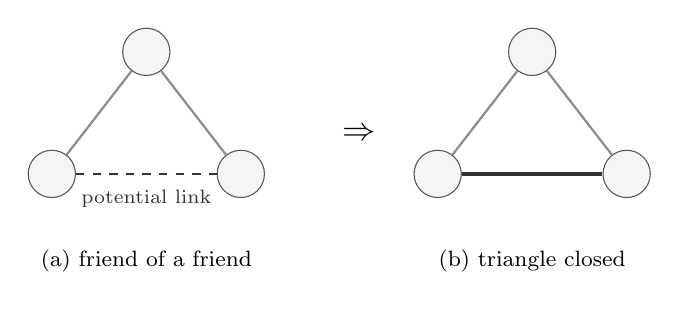
\begin{tikzpicture}[
  nd/.style={circle,draw=black!65,fill=black!4,minimum size=6mm,inner sep=0pt},
  lnk/.style={draw=black!45,line width=0.8pt},
  pot/.style={draw=accent,line width=1.0pt,dashed},
  newl/.style={draw=accent,line width=1.5pt}]
  % panel (a)
  \begin{scope}
    \node[nd] (A) at (0,1.15)    {};
    \node[nd] (B) at (-1.2,-0.4) {};
    \node[nd] (C) at (1.2,-0.4)  {};
    \draw[lnk] (A)--(B);
    \draw[lnk] (A)--(C);
    \draw[pot] (B)--(C);
    \node[accent,font=\scriptsize] at (0,-0.72) {potential link};
    \node[font=\footnotesize] at (0,-1.5) {(a) friend of a friend};
  \end{scope}
  \node at (2.7,0.1) {\large $\Rightarrow$};
  % panel (b)
  \begin{scope}[xshift=4.9cm]
    \node[nd] (A2) at (0,1.15)    {};
    \node[nd] (B2) at (-1.2,-0.4) {};
    \node[nd] (C2) at (1.2,-0.4)  {};
    \draw[lnk] (A2)--(B2);
    \draw[lnk] (A2)--(C2);
    \draw[newl] (B2)--(C2);
    \node[font=\footnotesize] at (0,-1.5) {(b) triangle closed};
  \end{scope}
\end{tikzpicture}\end{adjustbox}
\caption{\textbf{Triadic closure.} Two people (bottom) who already share a common
friend (top) form a \emph{potential link} --- a friend-of-a-friend pair, drawn
dashed. Closing the triangle turns that potential link into a real one, the
elementary step by which the friends-of-friends rule builds social structure.}
\label{fig:fr-closure}
\end{figure}

Figure~\ref{fig:fr-closure} shows this elementary step. Notice that it is a
thoroughly \emph{local} rule. To introduce two friends you
need to know only one node and its neighbors: who you know, and who they know.
That is exactly the kind of local information this book is built on, and the
question, as always, is what such a rule produces in the aggregate. The answer,
worked out below following \citet{vazquez2003} and reviewed in
\citet{vazquez2025}, is that connecting friends-of-friends generates the whole
suite of social-network signatures at once: an effective ``rich get richer'' and
hence a power-law degree distribution, the clustering hierarchy in which
cliquishness falls with degree, and --- in pointed contrast to the technological
and biological networks of the other chapters --- \emph{assortative} degree
correlations, the tendency of well-connected people to know one another.

Models in this spirit have a history. \citet{davidsen2002} introduced an
acquaintance-network model (the DEB model, after its authors) in which people are
repeatedly introduced to friends of friends, producing a small world with high
clustering; \citet{holme2002} bolted an explicit triangle-forming step onto
preferential attachment to give it tunable clustering. What follows organizes
these ideas around a single bookkeeping device that makes the mechanism
transparent --- the \emph{potential link}.

\section{Potential links}

The key idea is that, under triadic closure, a pair of nodes is not just
``connected'' or ``not connected.'' A pair that already shares a common neighbor
is a triangle waiting to close --- a candidate in a way that an arbitrary pair of
strangers is not. So we sort every pair of nodes into one of three states:
\begin{itemize}
  \item \emph{disconnected} ($s$): no link and no common neighbor --- two
    strangers with no mutual acquaintance;
  \item connected by a \emph{potential link} ($p$): no link yet, but at least one
    common neighbor --- two friends-of-a-friend, poised to be introduced;
  \item connected by a \emph{link} ($e$): already friends.
\end{itemize}
The \emph{potential link} is the formal stand-in for ``friend of a friend.'' We
write $k_i$ for the ordinary degree of node $i$ (its number of friends) and
$k^*_i$ for its \emph{potential degree}, the number of friends-of-friends it has
--- the number of potential links waiting at it.

Triadic closure is then a story about a pair changing state: a potential link
($p$) becomes a real link ($e$) when the triangle closes. To track this we need
to know the rates at which pairs hop between the three states, and one
relationship among those rates is the mechanical heart of the model. It says
that potential links are born in proportion to a node's degree --- introduce
yourself to someone with many friends and you instantly acquire many
friends-of-friends. The next box sets up the bookkeeping and draws out its main
consequence; the conclusion is restated plainly afterward, so the box may be
skipped.

\begin{calculation}{from the three-state bookkeeping to ``rich get richer''}
Let $\nu_{x\to y}$ be the rate (per unit of network size $n$) at which a pair
hops from state $x$ to state $y$. Ignoring fluctuations, the average degree and
potential degree of node $i$ evolve as
\begin{align}
  n\,\frac{\partial k_i}{\partial n}
    &= \nu_{s\to e}\,\hat k_i + \nu_{p\to e}\,k^*_i
       - (\nu_{e\to s}+\nu_{e\to p})\,k_i, \nonumber\\
  n\,\frac{\partial k^*_i}{\partial n}
    &= \nu_{s\to p}\,\hat k_i + \nu_{e\to p}\,k_i
       - (\nu_{p\to s}+\nu_{p\to e})\,k^*_i,
  \label{eq:fr-master}
\end{align}
where $\hat k_i = n - k_i - k^*_i$ is the number of nodes that are neither
friends nor friends-of-friends of $i$. The link between the two kinds of
connection comes from the geometry of triangles: when a new node $i$ attaches to
an existing node $j$, it instantly shares the common neighbor $j$ with \emph{all}
of $j$'s neighbors, gaining a potential link to each. Hence potential links are
spawned in proportion to degree,
\begin{equation}
  \nu_{s\to p} = \nu_{s\to e}\, k_i, \qquad
  \nu_{p\to s} = \nu_{e\to s}\, k_i.
  \label{eq:fr-coupling}
\end{equation}
Now make two modeling choices. First, neglect link deletion, $\nu_{e\to s}=0$ ---
accurate for, say, a co-authorship network, where having written a paper together
is a fact that cannot later become false. Second, make closing a triangle far
likelier than linking two strangers,
\begin{equation}
  \nu_{s\to e} = \frac{\mu_0}{n^2}, \qquad
  \nu_{p\to e} = \frac{\mu_1}{n},
  \label{eq:fr-rates}
\end{equation}
the stranger-linking rate carrying an extra factor of $1/n$. Substituting these
into Eq.~\eqref{eq:fr-master} collapses the system to
\begin{equation}
  n\,\frac{\partial k_i}{\partial n} = \mu_0 + \mu_1\, k^*_i, \qquad
  n\,\frac{\partial k^*_i}{\partial n} = \mu_0\, k_i - \mu_1\, k^*_i.
  \label{eq:fr-reduced}
\end{equation}
\end{calculation}

The upshot of Eq.~\eqref{eq:fr-reduced} is that a node's degree grows at a rate
proportional to how many friends-of-friends it has --- and a node with many
friends has, through them, many friends-of-friends. So once again the rich get
richer, but this time the preference is manufactured by triadic closure rather
than by surfing: a well-connected person is simply involved in more potential
introductions. As in the previous chapter, no node ever consulted a global
ranking; the bias toward hubs is a free by-product of a purely local act.

\section{Degree distribution and clustering hierarchy}

Because the growth rate is linear in degree, the same reasoning that gave a power
law in the last chapter applies here, and it simultaneously fixes the
cliquishness. The box carries out both; the two results and their meaning are in
the paragraph after it.

\begin{calculation}{the power law and the clustering hierarchy}
Integrating the linear system~\eqref{eq:fr-reduced} gives power-law growth of
both degrees with the age of the node,
\begin{equation}
  k_i(n) = k_0 \left(\frac{n}{n_i}\right)^{\beta}, \qquad
  k^*_i(n) = k^*_0 \left(\frac{n}{n_i}\right)^{\beta},
  \label{eq:fr-growth}
\end{equation}
where $n_i$ is the network size when node $i$ arrived and
\begin{equation}
  \beta = \frac{\mu_1}{2}\left(-1 + \sqrt{1 + 4\,\frac{\mu_0}{\mu_1}}\,\right).
  \label{eq:fr-beta}
\end{equation}
With nodes added at a constant rate, $P(n_i{=}n)=1/n$, a node has degree above $k$
only when it is old enough for Eq.~\eqref{eq:fr-growth} to exceed $k$; averaging
over its birth time gives the cumulative distribution
\begin{equation}
\adjustbox{max width=\linewidth}{$\displaystyle
  P(k_i > k) = P\!\left[k_0\left(\frac{n}{n_i}\right)^{\beta} > k\right]
  = \int_0^n \frac{dn_i}{n}\,
    \Theta\!\left[k_0\left(\frac{n}{n_i}\right)^{\beta} - k\right]
$}
  \label{eq:fr-cumulative}
\end{equation}
with $\Theta[\cdot]$ the step function, $1$ when its bracket holds and $0$
otherwise. Differentiating it leaves a power-law degree distribution,
\begin{equation}
  p_k = \frac{\partial P(k_i > k)}{\partial k} \sim k^{-\gamma}, \qquad
  \gamma = 1 + \frac{1}{\beta}.
  \label{eq:fr-pk}
\end{equation}
For the clustering, the dominant way node $i$ gains a triangle is a potential
link closing: when the potential link from $i$ to $j$ (sharing neighbor $k$)
becomes real, $i$ gains both the neighbor $j$ and a link $j$--$k$ among its
neighbors. Thus $\partial e_i/\partial n = \nu_{p\to e}\,k^*_i = \mu_1 k^*_i/n$,
and integrating with Eq.~\eqref{eq:fr-growth},
\begin{equation}
  \langle c\rangle_k = \frac{2 e(k)}{k(k-1)} \approx \frac{2\mu_1}{k}.
  \label{eq:fr-ck}
\end{equation}
\end{calculation}

Two familiar results emerge. First, Eq.~\eqref{eq:fr-pk}: the degree
distribution is again a power law. It is worth knowing exactly where the power
law comes from --- it comes from the proportionality in
Eq.~\eqref{eq:fr-coupling}, the fact that potential links are spawned in
proportion to degree. Were they instead spawned at a flat rate, the mechanism
would still create triangles but the degree distribution would decay
exponentially, with no fat tail of hubs. Scale-freeness is the fingerprint of
that degree-proportional spawning. Second, Eq.~\eqref{eq:fr-ck}: cliquishness
again falls as one over the degree --- the clustering hierarchy of the
introduction, now arriving by a third route (after search, and before
duplication in the next chapter). Here its origin is especially vivid: every
triangle a node owns is just a friend-of-a-friend pair that has been introduced.

\section{Connecting nearest neighbors}

The continuum theory is borne out by a minimal simulation, a growing version of
the DEB rule \citep{davidsen2002}. Starting from a single node and no links,
repeat:
\begin{itemize}
  \item with probability $1-u$, \emph{add} a new node and link it to a randomly
    chosen node $j$ --- which by definition creates a potential link between the
    newcomer and every neighbor of $j$;
  \item with probability $u$, \emph{close} a triangle: pick a potential link at
    random and turn it into a real link.
\end{itemize}
The single dial $u$ is the rate of triangle-closing relative to adding newcomers.
Feeding the mapping $\mu_0=1$, $\mu_1=u/(1-u)$ into the formulas above gives the
exponent in closed form, as the short box records.

\begin{calculation}{the exponent as a function of the closure rate}
With $\mu_0=1$ and $\mu_1=u/(1-u)$, Eqs.~\eqref{eq:fr-beta} and~\eqref{eq:fr-pk}
give
\begin{equation}
  \gamma(u) = 1 + \frac{2(1-u)}{u}
    \left(-1 + \sqrt{1 + 4\,\frac{1-u}{u}}\,\right)^{-1},
  \label{eq:fr-gammau}
\end{equation}
with limiting values
\begin{equation}
  \gamma(0) = \infty, \qquad \gamma(1) = 2.
  \label{eq:fr-limits}
\end{equation}
\end{calculation}

In words, the exponent is tunable by how eagerly the network closes triangles.
When closure is frequent and newcomers rare ($u\to 1$) the exponent sinks to its
minimum of $2$, the most hub-dominated case; when newcomers arrive so fast that
triangles never get a chance to close ($u\to 0$) the exponent blows up and the
heavy tail of hubs is lost. Simulations up to a million nodes confirm the
power-law degree distribution (the mean-field formula slightly overestimating the
exponent, as in the previous chapter), and they confirm the clustering hierarchy,
with cliquishness falling as a power of degree.

\section{Why social networks are assortative}

The most telling prediction is about the degree correlations --- and here the
friends-of-friends rule parts company with every other rule in this book.
Measuring the average neighbor degree $\langle k_{nn}\rangle(k)$ in the simulated
network, one finds it \emph{rises} with degree: the well-connected are connected
to the well-connected. The network is \emph{assortative}
\citep{newman2002} --- ``birds of a feather'' --- exactly as measured in real
collaboration and co-authorship networks, and exactly opposite to the
disassortative Internet and protein networks of the introduction.

Why the opposite sign? The reason becomes obvious once seen. Every new link here
closes a triangle, joining two nodes that share a common neighbor. But a node
that serves as the common neighbor of many pairs is, by definition, a high-degree
node, and the two nodes it brings together are drawn from its own neighborhood,
which is better connected than the network at large. So closure tends to wire
together nodes of \emph{similar}, and similarly high, degree. The very mechanism
that the disassortative models of the other chapters lack --- linking within a
neighborhood rather than reaching out to a random or peripheral node --- is what
tips the correlations positive. This is the deeper lesson of the chapter, and of
the review that develops it \citep{vazquez2025}: the \emph{sign} of the degree
correlations is not an arbitrary fitting knob but a direct readout of the
microscopic rule. Search and duplication reach outward, to the periphery, and so
make hubs that shun one another; triadic closure works inward, within
neighborhoods, and so makes hubs that keep each other's company.

\section{Summary}

Modeling social growth by triadic closure --- a newcomer attaches to a node and
then, over time, to that node's friends --- and formalizing ``friend of a friend''
as a \emph{potential link}, we obtain a tractable theory in which potential links
are created in proportion to degree. From that one ingredient follow an effective
``rich get richer,'' a power-law degree distribution with a tunable exponent
$\gamma = 1 + 1/\beta$, a clustering hierarchy in which cliquishness falls as one
over the degree, and --- distinctively --- assortative degree correlations.
Connecting friends-of-friends thus reproduces, from purely local moves, the
characteristic shape of social networks, and explains why the sign of their
correlations differs from that of the technological and biological networks
treated elsewhere in this book.


% instructions
% references
% - https://arxiv.org/abs/cond-mat/0211528, section IV
% 1- https://www.researchgate.net/publication/395472157_Degree_correlations_and_clustering_hierarchy_in_networks_measures_origin_and_consequences
%    Sub-chapter 4.2


\chapter{Gene duplication}
\label{ch:duplication}

\section{Networks that copy themselves}

The two rules of the preceding chapters each had a newcomer reach into the
existing network and \emph{choose} where to attach --- by surfing, or by closing
a triangle. Biology offers a third rule, and in some ways a more primitive one:
the network grows by \emph{copying} a node that is already there. The newcomer
does not pick its neighbors at all. It inherits them, wholesale, from a parent.

The setting is the inner machinery of the living cell. Genomes evolve in good
part through \emph{duplication} --- a gene, or sometimes an entire genome, is
accidentally copied --- followed by \emph{divergence}, the slow accumulation of
mutations that make the two copies drift apart. That duplication is a major
engine of evolution was argued classically by \citet{ohno1970}. To turn this into
a network statement we use the \emph{protein interaction network}: each node is a
protein (the product of a gene), and a link joins two proteins that physically
interact --- that bind to each other to do their job. Now watch what a gene
duplication does to this network. Right after the gene is copied, the cell makes
two identical proteins, so the new protein interacts with \emph{exactly the same
partners} as the old one: the duplicate node arrives already wired to all the
neighbors of its ancestor (Figure~\ref{fig:dup-diverge}). Mutations then add a few
interactions and, more often,
remove some, letting the twins diverge \citep{wagner2001,sole2002}. Both steps
are thoroughly local --- the copy needs to know only its parent and its parent's
neighbors, never the rest of the genome.

That moment just after the copy, when two proteins have \emph{exactly} the same
partners, is worth marking now because it turns out to matter far beyond the degree
statistics this chapter is about. Two nodes with identical neighborhoods are an exact
symmetry of the network, and Chapter~\ref{ch:quantum} shows that such a pair forces a
quantum walker to stay put: it pins an eigenvector of the walk onto the twins and
nowhere else. Duplication, in other words, does not merely shape how many links a
protein has. It plants a spectral signature that survives in the measured
interactome, and the same chapter finds real protein networks to be the most strongly
localized in this book.

\begin{figure}[t]
\centering
\begin{adjustbox}{max width=\linewidth}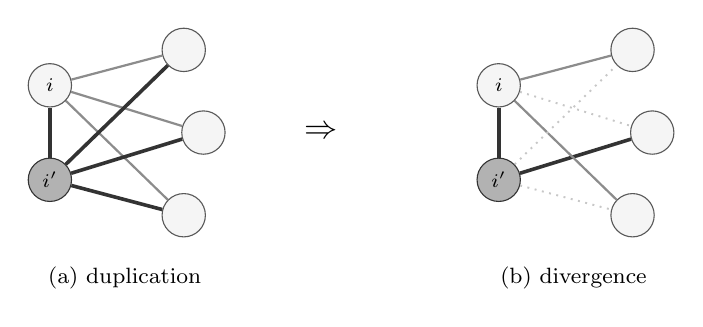
\begin{tikzpicture}[
  nd/.style={circle,draw=black!65,fill=black!4,minimum size=5.5mm,inner sep=0pt,font=\scriptsize},
  cp/.style={circle,draw=accent,fill=black!30,minimum size=5.5mm,inner sep=0pt,font=\scriptsize},
  lnk/.style={draw=black!45,line width=0.8pt},
  newl/.style={draw=accent,line width=1.3pt},
  gone/.style={draw=black!22,line width=0.7pt,dotted}]
  % panel (a) duplication
  \begin{scope}
    \node[nd] (i)  at (-0.2,0.6)  {$i$};
    \node[cp] (ip) at (-0.2,-0.6) {$i'$};
    \node[nd] (a)  at (1.5,1.05)  {};
    \node[nd] (b)  at (1.75,0.0)  {};
    \node[nd] (c)  at (1.5,-1.05) {};
    \draw[lnk]  (i)--(a); \draw[lnk] (i)--(b); \draw[lnk] (i)--(c);
    \draw[newl] (ip)--(a); \draw[newl] (ip)--(b); \draw[newl] (ip)--(c);
    \draw[newl] (i)--(ip);
    \node[font=\footnotesize] at (0.75,-1.85) {(a) duplication};
  \end{scope}
  \node at (3.25,0.0) {\large $\Rightarrow$};
  % panel (b) divergence
  \begin{scope}[xshift=5.7cm]
    \node[nd] (i2)  at (-0.2,0.6)  {$i$};
    \node[cp] (ip2) at (-0.2,-0.6) {$i'$};
    \node[nd] (a2)  at (1.5,1.05)  {};
    \node[nd] (b2)  at (1.75,0.0)  {};
    \node[nd] (c2)  at (1.5,-1.05) {};
    \draw[lnk]  (i2)--(a2);
    \draw[newl] (ip2)--(b2);
    \draw[lnk]  (i2)--(c2);
    \draw[newl] (i2)--(ip2);
    \draw[gone] (ip2)--(a2);
    \draw[gone] (i2)--(b2);
    \draw[gone] (ip2)--(c2);
    \node[font=\footnotesize] at (0.75,-1.85) {(b) divergence};
  \end{scope}
\end{tikzpicture}\end{adjustbox}
\caption{\textbf{Duplication and divergence.} (a) A gene duplication adds a copy
$i'$ (gray) wired to every interaction partner of the ancestor $i$, plus a link
between the twins when the protein is self-interacting. (b) Divergence then prunes
the now-redundant interactions (dotted), each partner kept by only one twin, so
the copies drift apart.}
\label{fig:dup-diverge}
\end{figure}

The same picture reaches beyond biology. A new web page is often made by copying
another page's hyperlinks and then editing the list --- duplication as copying,
divergence as editing. Following \citet{vazquez2003} and \citet{vazquez2003pin},
this chapter shows that copy-and-diverge, like the rules before it, produces an
effective ``rich get richer,'' a power-law degree distribution, the clustering
hierarchy, and --- as actually measured in protein networks \citep{maslov2002} ---
\emph{disassortative} correlations. It also reveals something new: a
\emph{multifractal} degree distribution, which we will unpack when we reach it, a
fingerprint left by the act of inheritance.

\section{Duplication and divergence, in their simplest form}

Start with the simplest version, treating duplication and divergence as
independent random events. The single idea that drives everything is this: a node
gains a new link whenever one of its \emph{neighbors} is duplicated, because the
neighbor's copy inherits a link back to it. A well-connected node has many
neighbors, so it has many chances to be on the receiving end of a duplication ---
and there, already, is the rich getting richer. The box makes this precise and
reads off the degree distribution; the conclusion follows it.

\begin{calculation}{degree growth and the power law from duplication}
In a mean-field (average-quantities) description, with increasing the number of
nodes $n$ the degree of node $i$ evolves as
\begin{equation}
  \frac{\partial k_i}{\partial n}
    = \nu_D\, k_i + \nu_C\,(n - k_i) - \nu_L\, k_i,
  \label{eq:dup-master}
\end{equation}
with $\nu_D$, $\nu_C$, $\nu_L$ the per-node rates of duplication, random link
creation, and link loss. The first term is the key one: it is proportional to
$k_i$ because each of $i$'s $k_i$ neighbors, if duplicated, hands $i$ a new link.
Each duplication adds one node, so $\nu_D = 1/n$; writing $\nu_C=\mu_0/n$ and
$\nu_L=\mu_1/n$ reduces the equation to
\begin{equation}
  n\,\frac{\partial k_i}{\partial n} = \mu_0 + (1-\mu_1)\, k_i,
  \label{eq:dup-reduced}
\end{equation}
whose growth rate is linear in the degree. Integrating it gives the degree of
node $i$ as the network grows,
\begin{equation}
  k_i(n) = \left(k_i(n_i) + \frac{\mu_0}{1-\mu_1}\right)
           \left(\frac{n}{n_i}\right)^{\beta} - \frac{\mu_0}{1-\mu_1},
  \label{eq:dup-growth}
\end{equation}
where $n_i$ and $k_i(n_i)$ are the network size and the node's degree at the
moment it was added, and the exponent is
\begin{equation}
  \beta = 1 - \mu_1 \qquad (\mu_1 < 1),
  \label{eq:dup-beta}
\end{equation}
the condition $\mu_1<1$ keeping the network from emptying out. To turn this growth
law into a degree distribution, note that node $i$ has degree above $k$ exactly
when its age and birth degree make Eq.~\eqref{eq:dup-growth} exceed $k$,
\begin{equation}
  P(k_i > k) = \Theta\!\left[\left(k_i(n_i) + \frac{\mu_0}{1-\mu_1}\right)
           \left(\frac{n}{n_i}\right)^{\beta} - \frac{\mu_0}{1-\mu_1} > k\right],
  \label{eq:dup-cumulative}
\end{equation}
with $\Theta[\cdot]$ the step function, $1$ when its bracket holds and $0$
otherwise.
Both its birth size $n_i$ and its birth degree $k_i(n_i)$ are random: for nodes
added at a constant rate $n_i$ is uniform, $P(n_i{=}n)=1/n$, while a node inherits
its ancestor's degree, so $P[k_i(n_i){=}k']=p_{k'}$ in the stationary state.
Averaging over both,
\begin{equation}
\adjustbox{max width=\linewidth}{$\displaystyle
  P(k_i > k) = \sum_{k'} p_{k'} \int_1^n \frac{dn_i}{n}\,
    \Theta\!\left[\left(k' + \frac{\mu_0}{1-\mu_1}\right)
           \left(\frac{n}{n_i}\right)^{\beta} - \frac{\mu_0}{1-\mu_1} > k\right]
$}
  \label{eq:dup-average}
\end{equation}
Differentiating this cumulative distribution and taking $n\gg1$ leaves,
for nodes added at a constant rate, a power-law degree distribution
\begin{equation}
  p_k = \frac{\partial P(k_i > k)}{\partial k}
      \sim \left(\frac{\mu_0}{1-\mu_1} + k\right)^{-\gamma}, \qquad
  \gamma = 1 + \frac{1}{1-\mu_1}.
  \label{eq:dup-pk}
\end{equation}
\end{calculation}

The result is once again a power law, Eq.~\eqref{eq:dup-pk}, and its exponent is
controlled entirely by $\mu_1$, the rate at which divergence removes links: the
more aggressively the duplicates shed interactions, the steeper the tail and the
fewer the giant hubs. As in the previous two chapters, the power law can be
traced to a single term that grows in proportion to degree --- here the
duplication term of Eq.~\eqref{eq:dup-reduced} --- and without it the distribution
would decay as a featureless exponential. Copying, all by itself, is a
rich-get-richer engine.

\section{Cliquishness from self-interaction}

If divergence added and removed links purely at random, this model would make no
triangles, and its cliquishness would fade to nothing in a large network. But
biology supplies one specific local source of triangles. Some proteins are
\emph{self-interacting} --- they bind to copies of themselves. When the gene for
such a protein is duplicated, the ancestor and its new twin can bind to
\emph{each other}, because each still carries the self-binding site
\citep{wagner2001}. That single interaction, laid down at the moment of
duplication, is the seed of a triangle. The short box turns this into the
clustering law.

\begin{calculation}{the clustering hierarchy from self-interaction}
Let a duplicated self-interacting protein bond to its ancestor with probability
$q_v$. Then whenever a neighbor of node $i$ is duplicated, $i$ gains not only the
copy as a new neighbor but, with probability $q_v$, a link between two of its
neighbors (the ancestor and the copy). Hence the number of links $e_i$ between the
neighbors of node $i$ change as
\begin{equation}
\frac{\partial e_i}{\partial n} \approx q_v\,\frac{\partial k_i}{\partial n}.
\end{equation}
Integrating, assuming $e_i=0$ when $k_i=1$, we get $e_i = q_v (k_i - 1)$.
Inserting this result into the clustering definition,
\begin{equation}
  \langle c\rangle_k = \frac{2 e(k)}{k(k-1)} \approx \frac{2 q_v}{k}.
  \label{eq:dup-ck}
\end{equation}
\end{calculation}

So cliquishness again falls as one over the degree, Eq.~\eqref{eq:dup-ck} --- the
clustering hierarchy of the introduction, reached now by a third independent
route. There is one telling refinement: because removing an interaction also
destroys triangles, and the biggest hubs have the most triangles to lose,
divergence makes the clustering of high-degree nodes decay a little \emph{faster}
than one over the degree. That slightly-too-steep falloff is a small signature
that distinguishes duplication from the search and closure mechanisms.

\section{When duplication and divergence are coupled}

In a real protein network the two processes cannot truly be independent. The
network does a job --- it keeps the cell alive --- so losing the wrong interaction
can be lethal, and which links a duplicate keeps is under natural selection. The
classical view of \citet{ohno1970} lets one redundant copy decay freely; the more
modern \emph{subfunctionalization} picture of \citet{force1999} has the two
copies divide the ancestor's duties between them, each keeping part, together
keeping the whole. Either way the fates of the two copies' links are
\emph{coupled}: a shared interaction is far more likely to be retained by one
copy than dropped by both. To capture this, \citet{vazquez2003pin} use the
following rule. Starting from two connected nodes, repeat:
\begin{itemize}
  \item \emph{Duplication.} Pick a node $i$ at random and add a copy $i'$ joined
    to every neighbor of $i$; with probability $q_v$ also add the link $i$--$i'$
    (the self-interaction case).
  \item \emph{Divergence.} For each node $j$ now joined to both $i$ and $i'$,
    delete one of the two redundant links $(i,j)$ or $(i',j)$, at random, with
    probability $1-q_e$.
\end{itemize}
The divergence step touches only the \emph{redundant} pairs just created, and
that is what couples it to duplication. Genomic data showing that duplicates
diverge soon after they are born \citep{wagner2001} justify treating divergence
as finishing before the next duplication, so the node count $n$ doubles as a
clock. A related model with lopsided divergence is studied in \citet{vazquez2003}.

Coupling makes the large-scale behavior considerably richer, in two ways worth
previewing before the box. First, a single number --- the retention parameter
$q_e$ --- decides whether the network stays sparse or grows ever denser, with a
sharp switch between the two regimes. Second, the degree distribution is no
longer a plain power law but a \emph{multifractal} one. A quick word on that
term: a plain power law is described by one exponent, the same at every scale; a
multifractal is described by a whole continuum of exponents, because different
``moments'' of the distribution (the average degree, the average of the squared
degree, and so on) scale with different powers of the network size. The box
records the transition and the moment exponents; the interpretation follows.

\begin{calculation}{the density transition and the multifractal spectrum}
Tracking the mean degree through one duplication event gives
\begin{equation}
\adjustbox{max width=\linewidth}{$\displaystyle
  \langle k\rangle(n+1)
   = \frac{n\langle k\rangle(n) + 2q_v + (2q_e - 1)\langle k\rangle(n)}{n+1}
$}
  \label{eq:dup-meandeg}
\end{equation}
which in the large-network limit switches behavior at $q_e=1/2$: for $q_e<1/2$
the mean degree saturates at the finite value $\langle k\rangle = 2q_v/(1-2q_e)$,
while for $q_e>1/2$ it grows without bound as $N^{2q_e-1}$. A rate-equation
treatment in the manner of \citet{kim2002} gives an attachment rate
$A(k)=(q_v+q_e k)/n$ --- linear in degree again --- and predicts that the $l$-th
moment of the degree distribution scales as $M_l\sim n^{\sigma_l(q_e)}$ with
\begin{equation}
  \sigma_l(q_e) = l\, q_e + 2\left[\left(\frac{1+q_e}{2}\right)^{l} - 1\right].
  \label{eq:dup-moments}
\end{equation}
For each $l$ there is a value $q_l$ at which $\sigma_l$ changes sign, with
$q_1=1/2$ and $q_2 = 2\sqrt{3}-3 \approx 0.46$.
\end{calculation}

The two messages of the box are these. First, Eq.~\eqref{eq:dup-meandeg} shows a
genuine switch at $q_e=1/2$: keep too few links and the network settles into a
sparse steady state; keep enough and it densifies forever. Second, and more
subtle, the moment exponents $\sigma_l$ in Eq.~\eqref{eq:dup-moments} depend on
$l$ in a curved, \emph{nonlinear} way --- the hallmark of a multifractal. Where
the earlier chapters gave clean single power laws, duplication gives a spectrum
of exponents, and the reason is exactly the inheritance at its core: each
newcomer copies the degree environment of its parent, injecting a kind of
heritable heterogeneity that a single exponent cannot capture. The deletion of
links from the copies is what converts that inheritance into multifractality.

\section{Disassortative correlations}

Simulations spanning network sizes from a thousand to a million nodes confirm the
analysis \citep{vazquez2003pin, vazquez2003}: the moment exponents match the multifractal prediction; the clustering
falls with degree as a power law with exponent at or above one (steepening as
link loss grows, just as Eq.~\eqref{eq:dup-ck} and its caveat foretold); and the
average neighbor degree \emph{decreases} with degree, $\langle k_{nn}\rangle(k)
\sim k^{-0.1}$. The duplication network is therefore \emph{disassortative} --- its
hubs are surrounded by poorly-connected partners rather than by each other.

This is the correct sign. Disassortative mixing is precisely what
\citet{maslov2002} measured in the protein interaction network of yeast, and it
files duplication alongside the technological networks of
Chapter~\ref{ch:search} and against the social networks of
Chapter~\ref{ch:friends}. With this third mechanism in hand, the three rules of
the book so far bracket the empirical landscape, as the table summarizes (here
$\beta$ is the rate at which cliquishness falls with degree, and $\alpha$ the
slope of the neighbor-degree curve --- positive for assortative, negative for
disassortative):
\begin{center}
\begin{tabular}{lcc}
\hline
Mechanism & $\langle c\rangle_k \sim k^{-\beta}$ & $\langle k_{nn}\rangle_k \sim k^{\alpha}$ \\
\hline
Connecting neighbors    & $0 < \beta < 1$ & $\alpha > 0$ \\
Random walk             & $\beta = 1$     & $\alpha \le 0$ \\
Duplication--divergence & $\beta \ge 1$   & $\alpha < 0$ \\
\hline
\end{tabular}
\end{center}
Every local rule produces a clustering hierarchy; what differs is the \emph{sign}
of the correlations, which sorts the rules into the assortative (social,
closure-driven) and disassortative (technological and biological, reach-driven)
classes seen in real data.

\section{The unifying principle}

Three different stories --- surfing a network, closing a triangle, copying a node
--- have each delivered the same effective ``rich get richer.'' That is no
accident, and the duplication picture makes the reason simple enough to state in
a single sentence.

Picking a node \emph{at random} plays no favorites: every node is equally likely,
hub or not. But none of the local rules in this book act on a randomly chosen
node. They act on a \emph{neighbor} of one --- the page a surfer steps to, the
friend a friend introduces, the partner a duplicated gene inherits. And the
chance that a particular node $i$ is the neighbor of a randomly chosen node is
\begin{equation}
  \frac{k_i}{\sum_j k_j},
  \label{eq:dup-unifying}
\end{equation}
which is exactly the linear preferential-attachment probability of the
Barab\'asi--Albert model \citep{barabasi1999}. High-degree nodes are
over-represented among the neighbors of a random node for the most elementary of
reasons: they belong to more neighborhoods, so more random nodes have them as a
neighbor. Preferential attachment never has to be imposed. It is induced
automatically the instant a growth rule takes one step out from a random node to
one of its neighbors. The clustering hierarchy has the same local root --- a rule
that makes one link to a node tends to make another among that node's neighbors
--- and the sign of the degree correlations depends on \emph{which} neighbor gets
chosen. Locality is the common cause, and the three mechanisms are three faces of
it.

\section{Summary}

Biological networks grow by duplication: a node is copied along with its
connections, and the copies then diverge by gaining and losing links. Because a
node gains a link whenever one of its neighbors is duplicated, the rule builds in
an effective ``rich get richer'' and hence a power-law degree distribution, while
duplications of self-interacting proteins generate a clustering hierarchy that
link loss steepens. Coupling divergence to duplication adds a density transition
at $q_e=1/2$ and a multifractal degree distribution born of inheritance, and the
model reproduces the disassortative correlations measured in real protein
networks. Together with the two previous chapters, duplication completes a simple
and general principle: a growth rule that attaches to a \emph{neighbor} of a
randomly chosen node attaches preferentially by degree --- and so preferential
attachment, the clustering hierarchy, and degree correlations are all the generic
harvest of locality.

One consequence of the rule is left for the last chapter, because it is not a
statistic of degrees at all. The identical twin a duplication creates is an exact
symmetry, and Chapter~\ref{ch:quantum} turns that into a theorem about how far a
coherent walker can travel on such a network --- then measures eight real interactomes
and finds them confined more tightly than anything modelled here, though whether it is
duplication doing the confining is a question that chapter has to leave open.


% instructions
% references
% - https://arxiv.org/abs/cond-mat/0211528, section V

\chapter{Activity specialization}
\label{ch:projects}

\section{Projects as growing networks}

The duplication rule of the previous chapter was born in biology, but copying is
not a biological privilege. This chapter applies the same idea to a very
different system --- the schedule of a large engineering project --- and gets, in
return, a surprising practical payoff: an explanation of why big projects so
reliably run late.

A project schedule can be drawn as a network, called an \emph{activity network}.
Its nodes are the individual activities, or tasks, that make up the project, and
its links record \emph{precedence}: a link from activity $a$ to activity $b$
means $b$ cannot begin until $a$ is finished --- you cannot paint a wall before it
is built. Because work only flows forward in time, the network has no loops; in
the jargon it is a \emph{directed acyclic graph}, with starting activities (no
predecessors) and finishing activities (no successors). For such a network there
is one object that has ruled project management since the 1950s: the
\emph{critical path}. This is the longest chain of dependent activities running
from start to finish --- the route through the project with no slack anywhere
along it, so that delaying \emph{any} activity on it pushes back the whole
project's end date by the same amount \citep{kelley1959}. The manager's
time-honored prescription is therefore simple: watch the critical path, and
guard it at all costs.

And yet projects keep finishing late. A survey of more than ten thousand of them
found only a few percent delivered on time and on budget, and fifteen years of
improvements in management practice barely moved that figure
\citep{flyvbjerg2003}. This stubborn record hints that the critical path --- a
single one-dimensional thread --- may be the wrong thing to watch in schedules
that have grown into genuinely complex networks. Following
\citet{vazquezprojects2023}, this chapter grows such schedules from a local rule,
shows that the critical path \emph{shrinks toward irrelevance} as projects get
bigger, and relocates the real source of delay risk in the network as a whole.

\section{The duplication--split rule}

Where does a schedule come from? Not in one piece. A plan is \emph{refined}: a
coarse activity is broken into finer ones, again and again, until the plan is
detailed enough to execute. There are two natural ways to break an activity in
two, and they correspond to two kinds of work. This is our local rule, with a
single dial, the duplication probability $q$. Beginning from two activities in
series, repeat: pick an existing activity at random and, with probability $q$,
\emph{duplicate} it, otherwise \emph{split} it.
\begin{itemize}
  \item \emph{Duplication} (probability $q$). A \emph{generic} activity is split
    into two smaller activities that run \emph{in parallel} --- think of doubling
    a crew so two teams do the same kind of work at once. Both copies inherit
    \emph{all} the predecessors and \emph{all} the successors of the parent.
    Duplication \emph{widens} the schedule, adding parallel strands of work.
  \item \emph{Split} (probability $1-q$). A \emph{specialized} activity is cut
    into two activities run \emph{in sequence} --- one specialist does the first
    part and hands off to another who does the second. The parent keeps its
    predecessors, the new activity takes over its successors, and a link joins
    the two. Splitting \emph{lengthens} the schedule, extending a chain.
\end{itemize}
\begin{figure}[t]
\centering
\begin{adjustbox}{max width=\linewidth}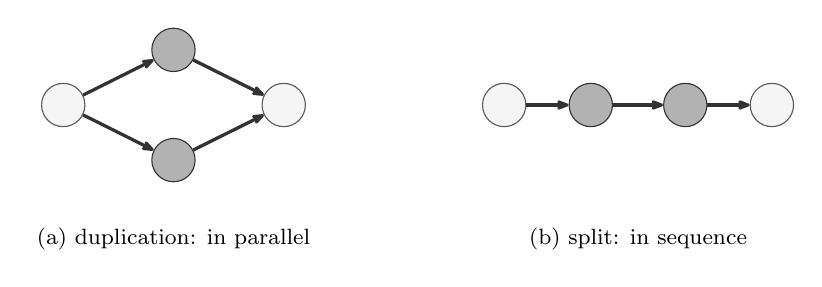
\begin{tikzpicture}[>={Stealth[round,length=2.2mm]},
  nd/.style={circle,draw=black!65,fill=black!4,minimum size=5.5mm,inner sep=0pt,font=\scriptsize},
  act/.style={circle,draw=accent,fill=black!30,minimum size=5.5mm,inner sep=0pt,font=\scriptsize},
  newl/.style={->,draw=accent,line width=1.2pt}]
  % panel (a) duplication: parallel
  \begin{scope}
    \node[nd]  (p)  at (0,0)      {};
    \node[act] (A1) at (1.4,0.7)  {};
    \node[act] (A2) at (1.4,-0.7) {};
    \node[nd]  (s)  at (2.8,0)     {};
    \draw[newl] (p)--(A1); \draw[newl] (p)--(A2);
    \draw[newl] (A1)--(s); \draw[newl] (A2)--(s);
    \node[font=\footnotesize] at (1.4,-1.7) {(a) duplication: in parallel};
  \end{scope}
  % panel (b) split: series
  \begin{scope}[xshift=5.6cm]
    \node[nd]  (p2) at (0,0)    {};
    \node[act] (B1) at (1.1,0)  {};
    \node[act] (B2) at (2.3,0)  {};
    \node[nd]  (s2) at (3.4,0)   {};
    \draw[newl] (p2)--(B1); \draw[newl] (B1)--(B2); \draw[newl] (B2)--(s2);
    \node[font=\footnotesize] at (1.7,-1.7) {(b) split: in sequence};
  \end{scope}
\end{tikzpicture}\end{adjustbox}
\caption{\textbf{Refining an activity.} A generic activity is replaced either by
(a) two copies that run \emph{in parallel}, both inheriting the predecessor (left,
gray) and successor (right, gray) of the parent --- duplication, which widens the
schedule --- or by (b) two specialized activities that run \emph{in sequence} --- a
split, which lengthens it.}
\label{fig:proj-dupsplit}
\end{figure}

So the dial $q$ measures how a project is organized (Figure~\ref{fig:proj-dupsplit}). Small $q$ means almost every
refinement is a split: work is broken into ever-longer chains of specialists, and
the schedule is nearly a single long line. Large $q$ means almost every
refinement is a duplication: generic work is parallelized into many simultaneous
strands, and the schedule fans out into a broad web. The same copying that
duplicated a gene in the previous chapter here duplicates an activity; the new
ingredient is the \emph{split} --- the act of \emph{specialization} that gives the
chapter its name --- and the forward-flowing, start-to-finish structure of a
schedule.

\section{Predecessors and successors: identical power laws}

Because the rule copies an activity together with its predecessors and
successors, it is a duplication rule of the kind that produced power-law degrees
in the previous chapter --- only now there are two degrees to track, the number of
predecessors (the in-degree) and the number of successors (the out-degree). The
box works out the distribution of predecessors by following how many activities
have each number of them; the same argument applies verbatim to successors. The
result is in the paragraph after.

\begin{calculation}{the distribution of predecessors}
Let $n_k(n)$ be the number of activities with $k$ predecessors when the schedule
has $n$ activities in all. Adding one activity changes this count by
\begin{equation}
\adjustbox{max width=\linewidth}{$\displaystyle
  n_k(n+1) = n_k(n)
   + q\left[\frac{k-1}{n}\,n_{k-1}(n) - \frac{k}{n}\,n_k(n)
            + \frac{1}{n}\,n_k(n)\right]
   + (1-q)\,\delta_{k,1}
$}
  \label{eq:proj-rate}
\end{equation}
the bracket collecting the duplication events (an activity climbs from $k-1$ to
$k$ predecessors when one of its predecessors is duplicated, and so on) and the
last term adding a fresh single-predecessor activity at each split. Looking for a
stable shape $n_k(n)=n\,p_k$ turns this into a recurrence,
\begin{equation}
  p_k = q\big[(k-1)\,p_{k-1} - k\,p_k + p_k\big] + (1-q)\,\delta_{k,1},
  \label{eq:proj-recurrence}
\end{equation}
which solves in closed form (with $\Gamma$ the gamma function) to
\begin{equation}
  p_k = \prod_{s=1}^{k-1}\frac{s}{\tfrac{1}{q}+s}\; p_1
      = \Gamma\!\left(\tfrac{1}{q}+1\right)
        \frac{\Gamma(k)}{\Gamma\!\left(\tfrac{1}{q}+k\right)}\, p_1,
  \label{eq:proj-pk}
\end{equation}
with the power-law tail
\begin{equation}
  p_k \sim k^{-1/q}.
  \label{eq:proj-asym}
\end{equation}
\end{calculation}

The result, Eq.~\eqref{eq:proj-asym}, is a power law with exponent $\gamma=1/q$.
A wide, duplication-heavy schedule (large $q$) has the heaviest tail of
highly-connected activities; at $q=1/2$ we recover the familiar value $\gamma=2$.
The very same reasoning, run on successors instead of predecessors, gives the
\emph{identical} distribution for the out-degree. That coincidence is the model's
signature prediction --- the spread of predecessor counts and the spread of
successor counts should look the same --- and it follows directly from the
even-handed way duplication treats the two ends of an activity.

\section{The vanishing critical path}

The degrees are a local property; the critical path is a global one. Remarkably,
the same rule fixes how the critical path grows with the size of the project, and
the answer overturns the manager's intuition. The box does the short
calculation; the consequences follow.

\begin{calculation}{how the critical path scales}
Let $c$ be the number of activities on the critical path of an $n$-activity
schedule. The path can only lengthen when a \emph{split} lands on it (a split
inserts an activity in series), and the chance that the activity picked for
refinement lies on the critical path is $c/n$. Hence
\begin{equation}
  \frac{dc}{dn} = (1-q)\,\frac{c}{n},
  \label{eq:proj-cp}
\end{equation}
which integrates to $c\sim n^{1-q}$, so the \emph{fraction} of activities on the
critical path shrinks as
\begin{equation}
  \frac{c}{n} \sim n^{-\alpha(q)}, \qquad \alpha(q) \le q.
  \label{eq:proj-cpfrac}
\end{equation}
Because distances here grow as a power of size, $c\sim n^{1/D}$, the network is a
\emph{fractal} with dimension
\begin{equation}
  D = \frac{1}{1-\alpha(q)}.
  \label{eq:proj-fractal}
\end{equation}
\end{calculation}

The headline is Eq.~\eqref{eq:proj-cpfrac}: for any amount of duplication
($q>0$), the critical path is a \emph{vanishing fraction} of the project as the
project grows. The bigger and more parallel the schedule, the smaller the slice
of the work that the manager's cherished path actually covers --- so watching the
critical path means watching an ever-shrinking sliver of the whole. (Simulations
confirm the power-law shrinkage, with the measured exponent $\alpha$ a little
below the simple bound $q$; for instance $\alpha\approx 0.11,\,0.28,\,0.43$ at
$q=0.20,\,0.50,\,0.70$.)

The scaling also tells us what \emph{kind} of network a schedule is. In a
small-world network, distances grow only logarithmically with size --- doubling
the network barely lengthens the longest path. Here distances grow as a
\emph{power} of size, the mark of a \emph{fractal} network: one whose ``size''
and ``length'' are tied together by a fixed dimension $D$, much as a physical
fractal looks the same at every magnification. Duplication--split schedules are
thus a class apart --- power-law degrees like a scale-free network, but power-law
(not logarithmic) distances, unlike a small world. Specialization builds the long
fractal chains; duplication stacks them up in parallel.

\section{Real project schedules}

This is not just a story about a model. \citet{vazquezprojects2023} examined
$77$ real construction projects, together worth more than ten billion dollars,
which yielded $323$ activity networks --- snapshots of projects at different
stages --- ranging from about a hundred to sixteen thousand activities. Three
predictions survive the encounter with data. First, the predecessor and successor
counts are each power-law distributed, and fitting them \emph{separately} yields
duplication indices $q$ that agree, just as the model demands they should.
Second, those indices fall between roughly $0.1$ and $0.5$, most above $0.2$:
real schedules sit on the split-dominated, nearly-linear side --- but with enough
duplication to matter. Third, the share of activities on the critical path falls
with project size right across the collection, confirming that the critical path
really does dwindle as projects grow.

\section{Delay risk as percolation}

If the critical path fades to insignificance and yet projects are still late,
where does the delay risk live? The answer is that it is spread across the whole
network, and it is governed by \emph{percolation} --- the same mathematics that
describes how water seeps through porous rock or how a forest fire spreads from
tree to tree.

Picture an outside shock --- bad weather, a strike, a pandemic --- that pushes
some activities past their planned finish. A delay only passes to a downstream
activity if it is large enough to use up the spare time, the \emph{free float},
built into that dependency; otherwise the buffer absorbs it and the delay stops
there. Now treat each dependency as a channel that passes a delay along with some
probability $p$, and ask what fraction of activities end up delayed beyond their
own slack --- the \emph{delay incidence}. This is exactly a percolation problem:
delays spread through the network of dependencies like fire through a forest, and
percolation theory says such spreading has a sharp \emph{threshold}
\citep{albert2000,ellinas2019,schwartz2002},
\begin{equation}
  p_c = \frac{1}{\langle k\rangle},
  \label{eq:proj-pc}
\end{equation}
where $\langle k\rangle$ is the average number of downstream dependencies per
activity. The meaning of a threshold is stark: below $p_c$ delays stay local and
project-wide overruns essentially never happen; above $p_c$ a finite fraction of
projects suffer a system-wide cascade --- the fire jumps the firebreaks.

The data choose between two stories cleanly. If the critical path governed
delay, the incidence ought to track $p\,c$ (transmission times critical-path
size); in the real projects that correlation is negligible. If percolation
governs delay, the incidence ought to switch on exactly at $p-p_c=0$; and that is
what the construction projects show --- below threshold, delay incidence stays
under one percent; above it, the incidence climbs, reaching fifteen percent of
all activities in the worst cases. The true control knob of project delay is
$p-p_c$, a property of the \emph{whole} network, not $p\,c$, a property of one
path through it.

Here is the chapter's practical lesson, and its link to the rest of the book. The
very same local rule that sets the degree distributions also sets the average
degree $\langle k\rangle$, and through Eq.~\eqref{eq:proj-pc} the threshold for
catastrophic delay. A project's tendency to run late is written into the network
its activities have grown into --- not into any single path through it.

\section{Summary}

Project schedules are forward-flowing networks of activities, grown by a local
refinement rule: pick an activity and either duplicate it into parallel copies
(probability $q$) or split it into specialized sequential parts. This
duplication--split rule predicts identical power-law distributions for the
numbers of predecessors and successors, $p_k\sim k^{-1/q}$; a critical path that
grows only as $c\sim n^{1-q}$ and so vanishes as a fraction of large projects;
and a fractal, rather than small-world, geometry. All three hold in $77$ real
construction projects. And because the critical path becomes irrelevant at scale,
delay risk is better read through percolation, with a threshold $p_c=1/\langle
k\rangle$ fixed by the grown network's average degree --- so that project
performance, in the end, is a property of the activity network as a whole.


% instructions
% references
% - https://www.nature.com/articles/s41598-022-27180-0

\chapter{Emergence of communities}
\label{ch:communities}

\section{Communities nobody designed}

So far the local rules of this book have explained the \emph{degree} structure of
networks --- their power laws, their clustering hierarchy, their correlations.
This chapter turns to a feature of an altogether different kind: \emph{community
structure}. A community is a group of nodes that are densely connected among
themselves but only sparsely connected to the rest of the network --- a clump
that hangs together. They are everywhere in real data: people fall into social
circles, web pages into topics, proteins into functional modules, each group
talking mostly to itself. Splitting a network into such groups is what
researchers mean by \emph{community detection}, and a network that splits cleanly
is said to have strong community structure.

Where do these communities come from? The usual answer points to differences
between the nodes themselves --- \emph{node heterogeneity}, in the jargon. People
of the same profession or politics, web pages on the same subject, proteins with
the same biological function: nodes of a kind, the story goes, are simply more
likely to link to one another, and that built-in preference is what carves the
network into groups. On this view, communities are stamped onto the network by
properties the nodes carried in from the start.

The thesis of this chapter, following \citet{vazquezcommunities2025}, is that no
such stamp is needed. \emph{Communities emerge from local growth rules even when
every node is identical.} The first hint is decades old: \citet{jin2001} showed
that a social network grown purely by triadic closure --- the friends-of-friends
rule of Chapter~\ref{ch:friends} --- develops communities although its nodes are
all of one type, and the same was later seen in the gene-duplication models of
Chapter~\ref{ch:duplication} \citep{sole2002}. If a featureless local rule
segregates a network into groups all by itself, then community structure joins
preferential attachment and the clustering hierarchy as one more thing that
\emph{emerges} from locality rather than being designed in.

To make that claim sharp we should ask it as a quantitative question, and the
right way to frame it comes from a corner of mathematics called \emph{Ramsey
theory}. Ramsey theory studies how large a random structure must become before
some orderly pattern is forced to appear. Its best-known nugget is a party fact:
in any gathering of six people, there are always either three who all know one
another or three who are all mutual strangers --- order of that kind is
unavoidable once the group is big enough. We will ask the analogous question of
growing networks: given a local growth rule, how large must the network become
before it is virtually \emph{certain} to contain communities? This chapter is, in
effect, a Ramsey theory of community structure in growing networks.

\section{The Ramsey community number}

Before we can measure when communities appear, we need a trustworthy way to
\emph{detect} them, and here some care is required, because the most popular
method can be fooled. That method, \emph{modularity optimization}, looks for the
division of a network that packs the most links inside groups; the trouble is
that it will happily report groups even in a completely random network that has
no real structure at all \citep{newman2006,fortunato2010}. To avoid being
deceived, the work relies instead on two more discerning tools: the
\emph{stochastic block model}, which fits the network to a statistical model of
blocks and keeps only the structure that genuinely earns its keep
\citep{karrer2011}, cross-checked against \emph{Infomap}, which finds groups by
watching where a random walker gets trapped \citep{rosvall2008}. Both, crucially,
report \emph{no} communities in a truly random network.

That last point also supplies the essential control. To be sure a community is
the work of the growth rule and not merely of the degrees, one compares the grown
network against a \emph{rewired} version of itself --- the links shuffled at
random while every node keeps its number of connections (this shuffling is called
the configuration model). If the communities survive the shuffle, they were never
more than an accident of the degrees; if they vanish, they were the doing of the
local rule. For every local model in this chapter, the shuffled version has no
communities at all --- so whatever structure we find is genuinely built by the
dynamics.

\begin{figure}[t]
\centering
\begin{adjustbox}{max width=\linewidth}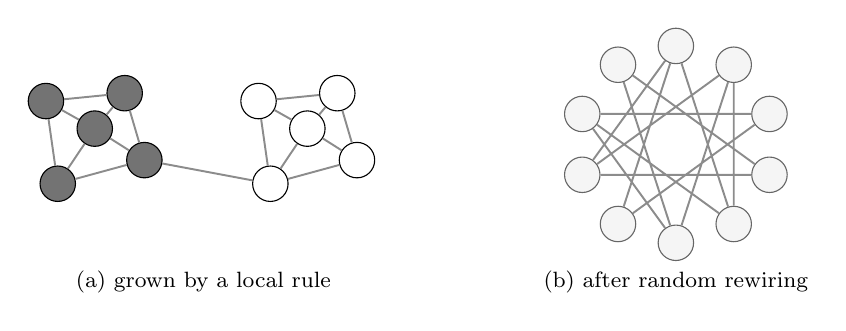
\begin{tikzpicture}[
  nd/.style={circle,draw=black!60,fill=black!4,minimum size=4.5mm,inner sep=0pt},
  cL/.style={circle,draw=black,fill=black!55,minimum size=4.5mm,inner sep=0pt},
  cR/.style={circle,draw=black,fill=white,minimum size=4.5mm,inner sep=0pt},
  lnk/.style={draw=black!45,line width=0.7pt}]
  % panel (a): two communities
  \begin{scope}
    \node[cL] (La) at (0.0,0.9)  {};
    \node[cL] (Lb) at (1.0,1.0)  {};
    \node[cL] (Lc) at (1.25,0.15){};
    \node[cL] (Ld) at (0.15,-0.15){};
    \node[cL] (Le) at (0.62,0.55){};
    \draw[lnk] (La)--(Lb) (La)--(Le) (La)--(Ld) (Lb)--(Lc)
               (Lb)--(Le) (Lc)--(Ld) (Lc)--(Le) (Ld)--(Le);
    \node[cR] (Ra) at (2.70,0.9)  {};
    \node[cR] (Rb) at (3.70,1.0)  {};
    \node[cR] (Rc) at (3.95,0.15) {};
    \node[cR] (Rd) at (2.85,-0.15){};
    \node[cR] (Re) at (3.32,0.55) {};
    \draw[lnk] (Ra)--(Rb) (Ra)--(Re) (Ra)--(Rd) (Rb)--(Rc)
               (Rb)--(Re) (Rc)--(Rd) (Rc)--(Re) (Rd)--(Re);
    \draw[lnk] (Lc)--(Rd);
    \node[font=\footnotesize] at (2.0,-1.4) {(a) grown by a local rule};
  \end{scope}
  % panel (b): rewired, no communities
  \begin{scope}[xshift=6.4cm]
    \foreach \i in {0,...,9}
      \node[nd] (d\i) at ({1.6+1.25*cos(90+36*\i)},{0.35+1.25*sin(90+36*\i)}) {};
    \draw[lnk] (d0)--(d4) (d0)--(d6) (d0)--(d3) (d1)--(d5) (d1)--(d7)
               (d2)--(d6) (d2)--(d8) (d2)--(d5) (d3)--(d7) (d3)--(d9)
               (d4)--(d8) (d5)--(d9) (d6)--(d9);
    \node[font=\footnotesize] at (1.6,-1.4) {(b) after random rewiring};
  \end{scope}
\end{tikzpicture}\end{adjustbox}
\caption{\textbf{Communities emerge from local rules.} (a) A network grown by a
local rule settles into dense communities (two here, one dark gray, one white) joined by
only a few links. (b) Shuffling the links at random while keeping every node's
number of connections destroys the communities --- so the structure was the work
of the rule, not of the degrees alone.}
\label{fig:com-rewire}
\end{figure}

With detection settled, we can pose the question precisely
(Figure~\ref{fig:com-rewire}). The box below states
the two definitions that do the work; both are short, and their meaning is given
in words right after, so the box can be skipped.

\begin{calculation}{the communities likelihood and the Ramsey community number}
For a growth rule $f_G$ that produces a network of $n$ nodes, let a detection
method $f_\kappa$ return the number $\kappa$ of communities it finds. Define the
\emph{communities likelihood} as the probability --- estimated by generating many
networks --- that an $n$-node instance has more than one community,
\begin{equation}
  P_\kappa(n) = \mathrm{Prob}\big\{\, \kappa \ge 2 \,\big\}.
  \label{eq:com-pk}
\end{equation}
The \emph{Ramsey community number} is then the smallest size at which communities
are all but guaranteed, at a confidence $1-\epsilon$ (we use $\epsilon=0.05$,
i.e.\ $95\%$):
\begin{equation}
  r_\kappa = \min\{\, n : P_\kappa(n) \ge 1-\epsilon \,\}.
  \label{eq:com-rk}
\end{equation}
A rule is said to have the \emph{emergent communities property} when such an
$r_\kappa$ exists.
\end{calculation}

In plain terms: $P_\kappa(n)$ is the chance that a network grown to size $n$ has
communities, and the Ramsey community number $r_\kappa$ is the size beyond which
that chance is essentially $(1-\epsilon)100\%$. A \emph{finite} $r_\kappa$ is the fingerprint
of emergence --- grow the network past it and communities are a near-certainty. A
rule for which no such size exists, no matter how large the network, simply does
not make communities on its own. The whole question ``do communities emerge from
this rule?'' thus reduces to ``is $r_\kappa$ finite?''

\section{Local rules grow communities}

We now line up two local rules against two controls. The local rules --- local
search and duplication--split, both met earlier in this book --- have the emergent
communities property; the controls --- reshuffling a network's links, and growing
one with no locality at all --- do not. Holding the four side by side is the whole
argument of the chapter in miniature.

\paragraph{Local search.} The model $\mathrm{LS}(n,d)$ is the search rule of
Chapter~\ref{ch:search} in undirected form \citep{vazquez2001}: each new node
takes a short walk of $d$ steps from a random starting node and links to every
node it visits. It carries preferential attachment and high clustering, and ---
though nothing in the rule ever mentions groups --- the block model resolves clear
communities, with $P_\kappa$ climbing from near zero around $n=10$ to a
near-certain one beyond about $n=100$, and staying there out to a hundred thousand
nodes \citep{vazquezcommunities2025}. Figure~\ref{fig:com-ls} shows one such network.

\begin{figure}[t]
\centering
\begin{adjustbox}{max width=\linewidth}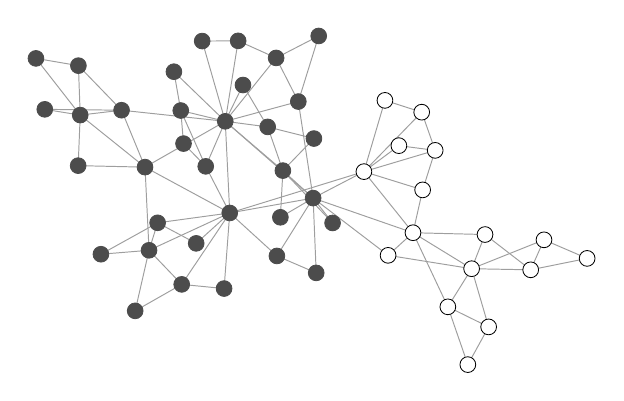
\begin{tikzpicture}[
  netlink/.style={draw=black!38,line width=0.35pt},
  nA/.style={circle,draw=black!70,fill=black!70,line width=0.3pt,inner sep=0pt,minimum size=0.20cm},
  nB/.style={circle,draw=black,fill=white,line width=0.3pt,inner sep=0pt,minimum size=0.20cm}]
  \draw[netlink] (3.520,2.115) -- (2.461,1.926);
  \draw[netlink] (3.520,2.115) -- (4.165,2.451);
  \draw[netlink] (3.520,2.115) -- (4.788,1.675);
  \draw[netlink] (3.520,2.115) -- (4.472,1.388);
  \draw[netlink] (3.520,2.115) -- (2.404,3.090);
  \draw[netlink] (3.520,2.115) -- (3.136,2.464);
  \draw[netlink] (3.520,2.115) -- (3.332,3.341);
  \draw[netlink] (3.520,2.115) -- (3.767,1.799);
  \draw[netlink] (3.520,2.115) -- (3.060,1.380);
  \draw[netlink] (3.520,2.115) -- (3.559,1.165);
  \draw[netlink] (3.520,2.115) -- (3.104,1.871);
  \draw[netlink] (2.461,1.926) -- (4.165,2.451);
  \draw[netlink] (2.461,1.926) -- (2.404,3.090);
  \draw[netlink] (2.461,1.926) -- (1.385,2.508);
  \draw[netlink] (2.461,1.926) -- (2.156,2.518);
  \draw[netlink] (2.461,1.926) -- (1.436,1.452);
  \draw[netlink] (2.461,1.926) -- (3.060,1.380);
  \draw[netlink] (2.461,1.926) -- (1.545,1.801);
  \draw[netlink] (2.461,1.926) -- (1.851,1.019);
  \draw[netlink] (2.461,1.926) -- (2.035,1.540);
  \draw[netlink] (2.461,1.926) -- (2.389,0.966);
  \draw[netlink] (4.165,2.451) -- (4.788,1.675);
  \draw[netlink] (4.165,2.451) -- (4.911,2.219);
  \draw[netlink] (4.165,2.451) -- (5.070,2.721);
  \draw[netlink] (4.165,2.451) -- (4.899,3.206);
  \draw[netlink] (4.165,2.451) -- (4.432,3.356);
  \draw[netlink] (4.165,2.451) -- (4.609,2.781);
  \draw[netlink] (4.788,1.675) -- (4.472,1.388);
  \draw[netlink] (4.788,1.675) -- (5.533,1.218);
  \draw[netlink] (4.788,1.675) -- (4.911,2.219);
  \draw[netlink] (4.788,1.675) -- (5.231,0.734);
  \draw[netlink] (4.788,1.675) -- (5.703,1.652);
  \draw[netlink] (4.472,1.388) -- (5.533,1.218);
  \draw[netlink] (2.404,3.090) -- (1.385,2.508);
  \draw[netlink] (2.404,3.090) -- (1.087,3.231);
  \draw[netlink] (2.404,3.090) -- (3.136,2.464);
  \draw[netlink] (2.404,3.090) -- (2.156,2.518);
  \draw[netlink] (2.404,3.090) -- (3.332,3.341);
  \draw[netlink] (2.404,3.090) -- (2.943,3.019);
  \draw[netlink] (2.404,3.090) -- (3.050,3.895);
  \draw[netlink] (2.404,3.090) -- (2.629,3.551);
  \draw[netlink] (2.404,3.090) -- (2.568,4.112);
  \draw[netlink] (2.404,3.090) -- (1.839,3.227);
  \draw[netlink] (2.404,3.090) -- (2.111,4.109);
  \draw[netlink] (2.404,3.090) -- (1.752,3.720);
  \draw[netlink] (1.385,2.508) -- (1.087,3.231);
  \draw[netlink] (1.385,2.508) -- (0.562,3.169);
  \draw[netlink] (1.385,2.508) -- (1.436,1.452);
  \draw[netlink] (1.385,2.508) -- (0.536,2.527);
  \draw[netlink] (5.533,1.218) -- (5.231,0.734);
  \draw[netlink] (5.533,1.218) -- (5.703,1.652);
  \draw[netlink] (5.533,1.218) -- (5.749,0.479);
  \draw[netlink] (5.533,1.218) -- (6.283,1.204);
  \draw[netlink] (5.533,1.218) -- (6.452,1.585);
  \draw[netlink] (4.911,2.219) -- (5.070,2.721);
  \draw[netlink] (1.087,3.231) -- (0.562,3.169);
  \draw[netlink] (1.087,3.231) -- (0.539,3.797);
  \draw[netlink] (1.087,3.231) -- (0.112,3.242);
  \draw[netlink] (3.136,2.464) -- (3.767,1.799);
  \draw[netlink] (3.136,2.464) -- (2.943,3.019);
  \draw[netlink] (3.136,2.464) -- (3.530,2.871);
  \draw[netlink] (3.136,2.464) -- (3.104,1.871);
  \draw[netlink] (5.231,0.734) -- (5.749,0.479);
  \draw[netlink] (5.231,0.734) -- (5.485,0.000);
  \draw[netlink] (5.070,2.721) -- (4.899,3.206);
  \draw[netlink] (5.070,2.721) -- (4.609,2.781);
  \draw[netlink] (2.156,2.518) -- (1.839,3.227);
  \draw[netlink] (2.156,2.518) -- (1.874,2.807);
  \draw[netlink] (0.562,3.169) -- (0.539,3.797);
  \draw[netlink] (0.562,3.169) -- (0.536,2.527);
  \draw[netlink] (0.562,3.169) -- (0.112,3.242);
  \draw[netlink] (0.562,3.169) -- (0.000,3.889);
  \draw[netlink] (4.899,3.206) -- (4.432,3.356);
  \draw[netlink] (1.436,1.452) -- (1.545,1.801);
  \draw[netlink] (1.436,1.452) -- (1.851,1.019);
  \draw[netlink] (1.436,1.452) -- (0.825,1.402);
  \draw[netlink] (1.436,1.452) -- (1.260,0.683);
  \draw[netlink] (3.332,3.341) -- (3.050,3.895);
  \draw[netlink] (3.332,3.341) -- (3.591,4.174);
  \draw[netlink] (0.539,3.797) -- (0.000,3.889);
  \draw[netlink] (5.703,1.652) -- (6.283,1.204);
  \draw[netlink] (5.749,0.479) -- (5.485,0.000);
  \draw[netlink] (2.943,3.019) -- (2.629,3.551);
  \draw[netlink] (2.943,3.019) -- (3.530,2.871);
  \draw[netlink] (3.050,3.895) -- (2.568,4.112);
  \draw[netlink] (3.050,3.895) -- (3.591,4.174);
  \draw[netlink] (3.060,1.380) -- (3.559,1.165);
  \draw[netlink] (6.283,1.204) -- (6.452,1.585);
  \draw[netlink] (6.283,1.204) -- (7.000,1.349);
  \draw[netlink] (2.568,4.112) -- (2.111,4.109);
  \draw[netlink] (6.452,1.585) -- (7.000,1.349);
  \draw[netlink] (1.545,1.801) -- (0.825,1.402);
  \draw[netlink] (1.545,1.801) -- (2.035,1.540);
  \draw[netlink] (1.851,1.019) -- (2.389,0.966);
  \draw[netlink] (1.851,1.019) -- (1.260,0.683);
  \draw[netlink] (1.839,3.227) -- (1.752,3.720);
  \draw[netlink] (1.839,3.227) -- (1.874,2.807);
  \node[nA] at (3.520,2.115) {};
  \node[nA] at (2.461,1.926) {};
  \node[nB] at (4.165,2.451) {};
  \node[nB] at (4.788,1.675) {};
  \node[nB] at (4.472,1.388) {};
  \node[nA] at (2.404,3.090) {};
  \node[nA] at (1.385,2.508) {};
  \node[nB] at (5.533,1.218) {};
  \node[nB] at (4.911,2.219) {};
  \node[nA] at (1.087,3.231) {};
  \node[nA] at (3.136,2.464) {};
  \node[nB] at (5.231,0.734) {};
  \node[nB] at (5.070,2.721) {};
  \node[nA] at (2.156,2.518) {};
  \node[nA] at (0.562,3.169) {};
  \node[nB] at (4.899,3.206) {};
  \node[nA] at (1.436,1.452) {};
  \node[nA] at (3.332,3.341) {};
  \node[nA] at (0.539,3.797) {};
  \node[nA] at (3.767,1.799) {};
  \node[nB] at (5.703,1.652) {};
  \node[nB] at (5.749,0.479) {};
  \node[nB] at (4.432,3.356) {};
  \node[nA] at (2.943,3.019) {};
  \node[nA] at (3.050,3.895) {};
  \node[nA] at (0.536,2.527) {};
  \node[nA] at (2.629,3.551) {};
  \node[nA] at (3.060,1.380) {};
  \node[nA] at (0.112,3.242) {};
  \node[nB] at (6.283,1.204) {};
  \node[nA] at (2.568,4.112) {};
  \node[nA] at (3.591,4.174) {};
  \node[nB] at (6.452,1.585) {};
  \node[nA] at (1.545,1.801) {};
  \node[nA] at (3.530,2.871) {};
  \node[nA] at (3.559,1.165) {};
  \node[nA] at (1.851,1.019) {};
  \node[nA] at (0.825,1.402) {};
  \node[nA] at (0.000,3.889) {};
  \node[nB] at (7.000,1.349) {};
  \node[nA] at (1.839,3.227) {};
  \node[nA] at (2.111,4.109) {};
  \node[nA] at (2.035,1.540) {};
  \node[nB] at (4.609,2.781) {};
  \node[nA] at (2.389,0.966) {};
  \node[nA] at (1.752,3.720) {};
  \node[nA] at (3.104,1.871) {};
  \node[nA] at (1.260,0.683) {};
  \node[nB] at (5.485,0.000) {};
  \node[nA] at (1.874,2.807) {};
\end{tikzpicture}
\end{adjustbox}
\caption{\textbf{Communities in a local-search network.} An instance of the
local-search model $\mathrm{LS}(n{=}50,d{=}1)$. The stochastic block model
resolves two communities, shown dark gray and white; they emerge even though the
rule treats every node alike and never mentions groups.}
\label{fig:com-ls}
\end{figure}

\paragraph{Duplication--split.} The model $\mathrm{DS}(n,q)$ is the undirected
cousin of the project-schedule rule of Chapter~\ref{ch:projects}: a new node
either copies all of a random node's links (probability $q$) or splits one of its
links in two. This model is the decisive case, because it builds \emph{no
triangles whatsoever} --- duplication makes none, and splitting destroys any that
might form --- and yet communities emerge just as reliably. The lesson is sharp: a
network does not need to be cliquish to have communities. What it needs is
locality, not triangles. Figure~\ref{fig:com-ds} shows an instance: two
communities, and not a triangle in sight.

\paragraph{Degree-preserving randomization.} To be sure the communities are the
work of the local rule and not of the degrees alone, we need a way to wipe out the
local structure while leaving every degree untouched. The \emph{configuration
model}, met when we defined the Ramsey number, does exactly that: it takes a
finished network and reshuffles its links at random, keeping each node's number of
connections fixed but scrambling \emph{which} nodes are joined. Applied to a
local-search or a duplication--split network, this reshuffling destroys the
communities outright --- the randomized versions have no finite Ramsey number at
all (the two ``randomized'' rows in the table below). Whatever the local rules
built, the bare list of degrees cannot sustain.

\paragraph{Barab\'asi--Albert.} Finally, $\mathrm{BA}(n,m)$ --- the canonical
preferential-attachment model --- is our \emph{non-local} control: a growing,
rich-get-richer network in which each newcomer attaches its $m$ links to nodes
drawn from the \emph{whole} graph, never once consulting a neighborhood. Despite
its growth and its rich-get-richer rule it has no emergent communities (the last
row of the table), and the next section is devoted to teasing apart exactly why.

\begin{figure}[t]
\centering
\begin{adjustbox}{max width=\linewidth}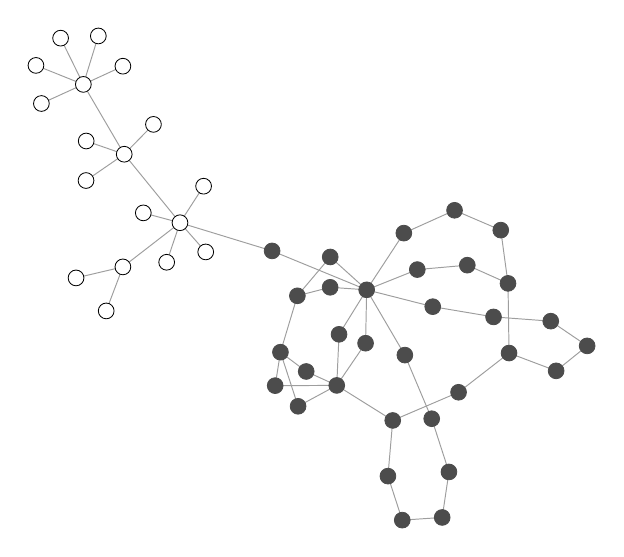
\begin{tikzpicture}[
  netlink/.style={draw=black!38,line width=0.35pt},
  nA/.style={circle,draw=black!70,fill=black!70,line width=0.3pt,inner sep=0pt,minimum size=0.20cm},
  nB/.style={circle,draw=black,fill=white,line width=0.3pt,inner sep=0pt,minimum size=0.20cm}]
  \draw[netlink] (1.363,3.902) -- (1.829,3.777);
  \draw[netlink] (1.829,3.777) -- (2.156,3.406);
  \draw[netlink] (1.829,3.777) -- (2.129,4.241);
  \draw[netlink] (1.829,3.777) -- (1.104,3.216);
  \draw[netlink] (1.829,3.777) -- (1.121,4.647);
  \draw[netlink] (1.829,3.777) -- (1.660,3.275);
  \draw[netlink] (1.829,3.777) -- (2.999,3.419);
  \draw[netlink] (4.531,1.266) -- (3.820,1.711);
  \draw[netlink] (4.531,1.266) -- (4.470,0.559);
  \draw[netlink] (4.531,1.266) -- (5.367,1.624);
  \draw[netlink] (5.159,0.034) -- (5.245,0.612);
  \draw[netlink] (5.159,0.034) -- (4.652,0.000);
  \draw[netlink] (4.200,2.925) -- (5.039,2.711);
  \draw[netlink] (4.200,2.925) -- (4.186,2.247);
  \draw[netlink] (4.200,2.925) -- (4.685,2.096);
  \draw[netlink] (4.200,2.925) -- (3.849,2.360);
  \draw[netlink] (4.200,2.925) -- (3.736,2.957);
  \draw[netlink] (4.200,2.925) -- (4.672,3.645);
  \draw[netlink] (4.200,2.925) -- (3.737,3.342);
  \draw[netlink] (4.200,2.925) -- (2.999,3.419);
  \draw[netlink] (4.200,2.925) -- (4.843,3.182);
  \draw[netlink] (0.892,2.657) -- (1.104,3.216);
  \draw[netlink] (5.039,2.711) -- (5.811,2.581);
  \draw[netlink] (0.792,6.149) -- (0.602,5.534);
  \draw[netlink] (1.104,3.216) -- (0.509,3.076);
  \draw[netlink] (1.121,4.647) -- (0.636,4.313);
  \draw[netlink] (1.121,4.647) -- (0.602,5.534);
  \draw[netlink] (1.121,4.647) -- (1.492,5.026);
  \draw[netlink] (1.121,4.647) -- (0.638,4.815);
  \draw[netlink] (4.186,2.247) -- (3.820,1.711);
  \draw[netlink] (3.820,1.711) -- (3.038,1.708);
  \draw[netlink] (3.820,1.711) -- (3.849,2.360);
  \draw[netlink] (3.820,1.711) -- (3.432,1.888);
  \draw[netlink] (3.820,1.711) -- (3.329,1.446);
  \draw[netlink] (4.685,2.096) -- (5.026,1.288);
  \draw[netlink] (3.320,2.849) -- (3.105,2.133);
  \draw[netlink] (3.320,2.849) -- (3.736,2.957);
  \draw[netlink] (3.320,2.849) -- (3.737,3.342);
  \draw[netlink] (0.602,5.534) -- (0.313,6.121);
  \draw[netlink] (0.602,5.534) -- (1.104,5.765);
  \draw[netlink] (0.602,5.534) -- (0.000,5.775);
  \draw[netlink] (0.602,5.534) -- (0.069,5.291);
  \draw[netlink] (5.245,0.612) -- (5.026,1.288);
  \draw[netlink] (4.470,0.559) -- (4.652,0.000);
  \draw[netlink] (3.105,2.133) -- (3.038,1.708);
  \draw[netlink] (3.105,2.133) -- (3.432,1.888);
  \draw[netlink] (3.105,2.133) -- (3.329,1.446);
  \draw[netlink] (6.008,2.122) -- (5.367,1.624);
  \draw[netlink] (6.008,2.122) -- (5.995,3.007);
  \draw[netlink] (6.008,2.122) -- (6.606,1.896);
  \draw[netlink] (5.478,3.238) -- (5.995,3.007);
  \draw[netlink] (5.478,3.238) -- (4.843,3.182);
  \draw[netlink] (5.995,3.007) -- (5.903,3.683);
  \draw[netlink] (5.811,2.581) -- (6.538,2.527);
  \draw[netlink] (7.000,2.213) -- (6.606,1.896);
  \draw[netlink] (7.000,2.213) -- (6.538,2.527);
  \draw[netlink] (4.672,3.645) -- (5.316,3.935);
  \draw[netlink] (5.316,3.935) -- (5.903,3.683);
  \node[nB] at (1.363,3.902) {};
  \node[nB] at (1.829,3.777) {};
  \node[nB] at (2.156,3.406) {};
  \node[nA] at (4.531,1.266) {};
  \node[nA] at (5.159,0.034) {};
  \node[nA] at (4.200,2.925) {};
  \node[nB] at (0.892,2.657) {};
  \node[nB] at (2.129,4.241) {};
  \node[nA] at (5.039,2.711) {};
  \node[nB] at (0.792,6.149) {};
  \node[nB] at (1.104,3.216) {};
  \node[nB] at (1.121,4.647) {};
  \node[nA] at (4.186,2.247) {};
  \node[nB] at (1.660,3.275) {};
  \node[nA] at (3.820,1.711) {};
  \node[nB] at (0.636,4.313) {};
  \node[nA] at (4.685,2.096) {};
  \node[nB] at (0.509,3.076) {};
  \node[nA] at (3.320,2.849) {};
  \node[nB] at (0.602,5.534) {};
  \node[nA] at (5.245,0.612) {};
  \node[nA] at (4.470,0.559) {};
  \node[nA] at (3.105,2.133) {};
  \node[nA] at (3.038,1.708) {};
  \node[nA] at (6.008,2.122) {};
  \node[nA] at (5.367,1.624) {};
  \node[nA] at (5.478,3.238) {};
  \node[nB] at (0.313,6.121) {};
  \node[nB] at (1.104,5.765) {};
  \node[nA] at (3.849,2.360) {};
  \node[nB] at (1.492,5.026) {};
  \node[nA] at (3.736,2.957) {};
  \node[nA] at (4.652,0.000) {};
  \node[nA] at (5.995,3.007) {};
  \node[nA] at (5.811,2.581) {};
  \node[nA] at (7.000,2.213) {};
  \node[nB] at (0.000,5.775) {};
  \node[nA] at (6.606,1.896) {};
  \node[nA] at (4.672,3.645) {};
  \node[nA] at (3.737,3.342) {};
  \node[nA] at (5.316,3.935) {};
  \node[nA] at (5.026,1.288) {};
  \node[nA] at (2.999,3.419) {};
  \node[nA] at (6.538,2.527) {};
  \node[nA] at (4.843,3.182) {};
  \node[nA] at (3.432,1.888) {};
  \node[nA] at (5.903,3.683) {};
  \node[nA] at (3.329,1.446) {};
  \node[nB] at (0.638,4.815) {};
  \node[nB] at (0.069,5.291) {};
\end{tikzpicture}
\end{adjustbox}
\caption{\textbf{Communities in a duplication--split network.} An instance of the
duplication--split model $\mathrm{DS}(n{=}50,q{=}0.3)$. Two communities (dark gray
and white) again emerge --- even though this rule builds no triangles at all, so the
network is far less cliquish than the local-search one of
Figure~\ref{fig:com-ls}.}
\label{fig:com-ds}
\end{figure}

A few representative Ramsey numbers, based on numerical estimates for $\epsilon=0.05$
\citep{vazquezcommunities2025}, make the pattern concrete:

\begin{center}
\begin{tabular}{lcc}
\hline
Model & $r_\kappa$ (block model) & $r_\kappa$ (Infomap) \\
\hline
$\mathrm{LS}(d=1)$               & $81$   & $222$  \\
$\mathrm{DS}(q=0.5)$             & $98$   & $622$  \\
$\mathrm{LS}(d=1)$, randomized   & ---    & ---    \\
$\mathrm{DS}(q=0.5)$, randomized & ---    & ---    \\
$\mathrm{BA}(m=2)$               & ---    & ---    \\
\hline
\end{tabular}
\end{center}
Every genuinely local rule has a finite Ramsey number --- grow it past a few
hundred nodes and communities are certain. The rules without local structure ---
the bottom three rows, the two reshuffled networks and the Barab\'asi--Albert
model --- have none: the dashes mean communities never become certain, however
large the network. The exact figures differ between the
two detection methods --- there is no single ``true'' definition of a community,
and where the line falls depends a little on how one draws it --- but the
\emph{split} between local rules (finite) and non-local ones (infinite) is the
same either way. Local structure is a necessary condition for communities to
emerge.

\section{When globality fails: the Barab\'asi--Albert model}

The natural control is the Barab\'asi--Albert model \citep{barabasi1999}, the
textbook growing network with \emph{no} locality at all: each newcomer attaches
its $m$ links to nodes chosen from the \emph{whole} network in proportion to
their degree. It has growth and preferential attachment, but no step that ever
looks at a node's neighborhood --- and it does \emph{not} have the emergent
communities property. Its community likelihood rises only to about one-half near
a thousand nodes and then \emph{falls} as the network grows further, never
reaching certainty. The little structure it has comes from the mere age-ordering
of its nodes, not from any local rule, and it washes out at scale.

The boundary case is illuminating. Give the model a baseline ``attractiveness''
$a$, so that a node is chosen with a probability proportional to $a +
k_i/\sum_j k_j$ --- a fixed head-start $a$ on top of the usual degree preference.
This tunes the degree exponent to $\gamma=2+a/m$. Tracking the Ramsey number
across these variants reveals a clean rule of thumb: communities emerge exactly
when the network is \emph{clustered} enough. The Ramsey number falls as the
average clustering coefficient rises, and \emph{diverges} --- communities never
become certain --- as the clustering goes to zero \citep{vazquezcommunities2025}. The standard Barab\'asi--Albert
model sits right at that vanishing point, because its clustering decays toward
zero as it grows (like $(\ln n)^2/n$): the bigger it gets, the fewer short cycles
it has, and short cycles are what local structure is made of. So even here the
principle holds --- where the dynamics happen to generate appreciable clustering
(an \emph{implicit} bit of local structure), communities appear; where clustering
fades, they do not.

\section{How local must ``local'' be?}

If locality is the cause, exactly how local must a connection be to count? Two
dials settle it: the length of the cycles a rule creates, and the distance it
reaches across. Triadic closure closes triangles (cycles of length three); the
duplication--split rule works with squares (length four). To sweep the cycle
length freely, use the \emph{bubble model}: at each step a chain of $L$ new nodes
is added and its two ends are attached to the two ends of a randomly chosen
existing link, creating a fresh cycle of length $L+2$. As $L$ grows --- as the
rule weaves ever longer cycles --- the Ramsey number climbs with it, and steeply:
from $r_\kappa=108$ for the shortest cycles to more than fifty thousand by $L=9$
\citep{vazquezcommunities2025}, as the table below records. The climb is not quite
smooth --- riding on top of it is a regular even--odd alternation, the odd-length
cycles bringing communities on sooner than the even cycles around them, an effect
plainest for the shorter cycles --- but the overall message is unmistakable: short
cycles, tight local feedback, bring communities on soonest.

\begin{center}
\begin{tabular}{ccc}
\hline
$L$ & cycle length $L+2$ & $r_\kappa$ \\
\hline
1 & 3  & 108 \\
2 & 4  & 326 \\
3 & 5  & 246 \\
4 & 6  & 2201 \\
5 & 7  & 752 \\
6 & 8  & 6595 \\
7 & 9  & 2740 \\
8 & 10 & 15863 \\
9 & 11 & 56160 \\
\hline
\end{tabular}
\end{center}

Distance matters just as much. In the bubble model the chain's two ends attach to
nodes that are a single step apart (the ends of one link). Loosen this so the
ends may attach to nodes up to $W$ steps apart, with the chain length fixed at
$L=1$. For $W=1$ communities still emerge with certainty, at $r_\kappa=108$;
stretching to $W=2$ pushes the threshold up roughly tenfold, to $r_\kappa=1090$,
but the communities still come. At $W=3$ --- and likewise if the ends are joined
to nodes picked anywhere at random --- they stop appearing altogether, the Ramsey
number ceasing to exist (the dash in the table) \citep{vazquezcommunities2025}.

\begin{center}
\begin{tabular}{cc}
\hline
$W$ & $r_\kappa$ \\
\hline
1 & 108 \\
2 & 1090 \\
3 & --- \\
\hline
\end{tabular}
\end{center}

For this model, ``local'' means roughly two steps: communities form
when new links reinforce ties among nearby nodes, and dissolve once links are
allowed to leap across the network. This is the whole book's premise made
quantitative. It is not growth, nor preferential attachment, nor even clustering
in the abstract that carves a network into communities --- it is the
\emph{locality} of the rule by which it grew.

\section{Summary}

Community structure, long blamed on built-in differences between nodes, is
instead something that \emph{emerges} from growing a network by local rules, even
when every node is identical. Made precise through the Ramsey community number
$r_\kappa$ --- the size beyond which communities are all but certain --- the
statement is clean: the local rules of earlier chapters (search and
duplication--split) have a finite $r_\kappa$, while their
degree-preserving shuffles, and the non-local Barab\'asi--Albert model, have none.
Triangles are not required (duplication--split makes none and still segregates),
but locality is: communities come soonest for rules that close short cycles
between nearby nodes, and disappear once links may span the whole network. Having
already accounted for degree distributions, the clustering hierarchy, and degree
correlations, this chapter adds community structure to the list of global
patterns that locality alone can explain \citep{vazquez2025}.


% instructions
% references
% - https://arxiv.org/abs/2501.17042

\chapter{The limit of a network}
\label{ch:graphons}

\section{A photograph of the whole}

The last chapter counted communities. It found that the number grows as a power
of the size, $B\propto n^{\beta}$ with $\beta\approx0.61$, and compared that
exponent with the $\sqrt{n}$ of the self-similar models. This chapter asks what
that comparison means, and the answer turns out to reach further than the
question.

Start with a way of looking at a network that we have not used yet. Draw its
adjacency matrix as a picture: one pixel for each pair of nodes, black if they
are linked, white if they are not. Order the nodes so that similar ones sit
together. Now grow the network and watch the picture. If the network is
\emph{dense} --- if each node links to a fixed \emph{fraction} of the others ---
the picture settles down. The individual pixels become too small to see, and what
survives is a pattern of greys: a smooth function $W(x,y)$ on the unit square
giving, for each pair of positions, the probability of a link
(Figure~\ref{fig:gr-limit}a). That limiting function is called a \emph{graphon},
and it is the object that a growing dense network converges to
\citep{lovasz2006,borgs2008}. Two networks with the same graphon are the same
network as far as any large-scale statistic can tell.

\begin{figure}[t]
\centering
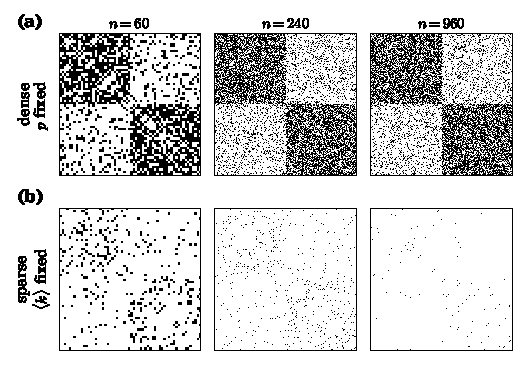
\includegraphics[width=\linewidth]{figs/fig-gr-limit.pdf}
\caption{\textbf{The limit picture, under two scalings.} Adjacency matrices of the
same two-block structure at $n=60$, $240$, $960$, nodes ordered by block.
(a)~Dense: the link probabilities are held fixed, and the picture sharpens onto a
step function --- the graphon. (b)~Sparse: the mean degree is held fixed instead,
so the probabilities fall as $1/n$. The structure is identical, and just as
detectable, but the picture fades to white. Real networks are of the second kind.}
\label{fig:gr-limit}
\end{figure}

This is a powerful idea, and it has a large and beautiful theory attached to it.
It is also, applied naively to the networks in this book, useless --- and the
precise way in which it fails is instructive. The reason is the second row of
Figure~\ref{fig:gr-limit}. Real networks are not dense. The Internet, the
interactome, a co-authorship graph, all keep a roughly fixed mean degree as they
grow; so does every model in this book. When the mean degree is fixed the link
probability falls like $1/n$, the pixels thin out, and the picture converges ---
to white. The limit exists, and it has thrown away everything we care about.

The obvious repair is to turn up the contrast: divide the whole picture by its
own average darkness before taking the limit, so that what survives is the
\emph{pattern} of the greys rather than their absolute level. This works, and it
is the substance of a theory of sparse graph limits developed by
\citet{borgs2019}. Rescaling costs something --- the rescaled function is no
longer a probability bounded by one, so the limit object is no longer a bounded
function but an $L^p$ one, and the theory must be rebuilt around that --- but the
gain is real. It is the first limit theory that copes with hubs, and with the
power-law degree distributions that come with them.

There are then three regimes, not two, and it is worth knowing which one a
network is in. Dense networks have ordinary bounded graphons. Networks that are
sparse but \emph{densifying} --- the link probability falling to zero while the
mean degree still creeps up --- have $L^p$ graphons. And networks of genuinely
fixed mean degree have neither. The rescaling that saves the middle case needs the
mean degree to grow without bound, and when it does not, the rescaled picture
concentrates instead of settling: for the ring it piles up along the diagonal,
approaching not a function but a line of infinite density.

Which regime a real system is in is a question with an answer, and the systems
followed through this book do not give the same one. Track the mean degree against
size and fit $\langle k\rangle\propto n^{\delta}$: the Internet at the
autonomous-system level, over $733$ snapshots, gives $\delta=-0.04$ --- flat, or
very slightly thinning, a mean degree that stays near four while the network grows
sixty-fold. That is the third regime, and no limit theory yet reaches it. The
cond-mat co-authorship network gives $\delta=+0.36$, and its mean degree climbs
from $2.2$ to $19$ as it grows from four hundred to four hundred thousand authors.
That is the middle regime: co-authorship densifies, and it is the one system here
that the $L^p$ theory actually covers.

The interactomes appear to densify too, more gently, but the appearance should not
be trusted: that series runs across \emph{organisms} rather than across time, and
a better-studied organism has both more proteins catalogued and more interactions
recorded per protein. The trend there measures the attention of biologists at
least as much as the architecture of cells.

Even the middle regime is tighter than it looks, in a way the book's own models
can measure. Membership in $L^p$ is a condition on how extreme the hubs are: for a
degree distribution $p(k)\sim k^{-\gamma}$ it holds when $p<\gamma-1$, and the
theory needs $p>1$, so there is a usable window only for $\gamma>2$. The
pseudofractal web of the last chapter has $\gamma\simeq2.585$, leaving the window
$1<p<1.585$; real networks, whose exponents cluster between two and three, are all
squeezed into the same narrow slot, and it closes entirely as $\gamma\to2$. The
limit theory reaches the scale-free world, but only just.

Being in the third regime is worth stating plainly, because it explains the shape
of the previous chapter. The evidence for a partition there grew like $m\ln K$, in
proportion to the number of \emph{links}; the graphon limit normalizes by the
number of \emph{pairs}, which is $n^2$. The two scales differ by the mean degree, and in
the sparse world that ratio is the whole story. It is why the last chapter had to
compute at finite $n$ and could not simply take a limit. The finite-size
calculation was not a convenience. It was the only instrument that sees anything.

\section{The block model was a graphon all along}
\label{sec:gr-blockmodel}

Set the difficulty aside for a moment, because the language is useful even where
the limit theorem is not.

A stochastic block model \emph{is} a graphon --- the simplest interesting kind. If
the nodes fall into blocks and the link probability depends only on which blocks
the endpoints are in, then $W$ is a step function: constant on each rectangle,
jumping at the block boundaries. Fitting a block model to a network is fitting a
step function to a picture, and asking how many blocks it needs is asking how
finely the picture must be pixelated before the description stops improving.

The degree-corrected model of the last chapter is a graphon too, and its shape
says exactly what degree correction \emph{does}.

\begin{calculation}{degree correction, as a factorization}
Let the graphon factorize as
\begin{equation}
  W(x,y) = f(x)\,f(y)\;w\big(g(x),g(y)\big),
  \label{eq:gr-factor}
\end{equation}
where $g(x)$ names the block at position $x$, $w$ is constant on block pairs, and
$f$ is an arbitrary non-negative function. The first two factors form a
\emph{rank-one} graphon: a product $f(x)f(y)$, in which a node's propensity to
link is a single number and nothing about \emph{whom} it links to. That is the
configuration model, and $f$ is the degree profile. Comparing with the discrete
version of the last chapter, $\theta_i=k_i/\sqrt{2m}$ is the empirical estimate of
$f$, and $\omega_{rs}$ is the block-constant residual $w$. Setting $w\equiv1$
recovers the pure degree model, which is exactly the statement made there that
$\omega_{rs}=1$ reproduces the configuration model.
\end{calculation}

So the two block models of the last chapter differ in one respect only: the
baseline they measure structure against. The plain model tests the network
against a \emph{constant} graphon; the degree-corrected model tests it against the
best \emph{rank-one} graphon. Degree correction is the removal of the rank-one
part, nothing more and nothing less.

Seen this way the pseudofractal reversal loses its strangeness. A degree-blind
model has no rank-one factor to spend, so the only way it can express a steep
degree gradient is through the block structure itself --- and it duly spends its
blocks on separating hubs from leaves, which is the hub--leaf cut it was found
preferring. Give it a rank-one factor and the gradient is absorbed there, leaving
the blocks free to describe what actually remains: the branch geometry. The
correction does not weaken the case for the branch cut because the branch cut was
never what the degrees were explaining.

The evidence itself has a graphon reading as well. The large-count form of the
degree-corrected evidence --- the sum of $e_{rs}\ln(e_{rs}/\Omega_{rs})$ over
block pairs, met in the last chapter --- is $m$ times a relative entropy between
the fitted residual $w$ and the flat one --- the same functional that governs large deviations for
random graphs \citep{chatterjee2011}. This sharpens a claim made in passing there.
The result $\log R_{\mathrm{dc}}/m\to\ln K$ was said to owe nothing to the diamond
lattice; now we can say why. Relative entropy is a property of the limiting shape,
not of the construction that produced it, and any arrangement of $K$ equal
well-separated blocks has the same one.

\section{How much can be seen}

Now to the question the last chapter raised without quite asking: what sets the
number of blocks?

Fitting a step function to a picture is a balancing act familiar from any
histogram. Too few bins and the description is crude --- real variation is
averaged away. Too many and each bin holds too little data to estimate, so the
description is noise. The optimum sits where the two costs meet, and it moves
with the amount of data. This is the classical bias--variance trade-off, and for
networks it has been worked out precisely.

\begin{calculation}{the cost of a $k$-block description}
Three terms compete. Smoothness here means the H\"older exponent: a graphon has
smoothness $\alpha$ if, for some constant $M$,
\begin{equation}
  |W(x,y)-W(x',y')| \;\le\; M\big(|x-x'|^{\alpha}+|y-y'|^{\alpha}\big),
  \label{eq:gr-holder}
\end{equation}
so that $\alpha=1$ is the Lipschitz case --- a surface of bounded slope --- and
smaller $\alpha$ lets it swing more violently over a short distance. The
\emph{approximation} error of describing such a surface by $k$ steps then follows
in a line: cover the square with $k\times k$ cells of side $1/k$ and fit a constant
on each; two points in a cell are at most $1/k$ apart, so
Eq.~\eqref{eq:gr-holder} caps the deviation inside it at $Mk^{-\alpha}$, and since
the risk is a mean \emph{squared} error, squaring gives $k^{-2\alpha}$. Against it
run two estimation costs, established by
\citet{gao2015}: a term $k^2/n^2$ for fitting the $k^2$ block parameters
themselves, and a term $n^{-1}\ln k$ for the harder problem of not knowing which
node belongs to which block. The total is
\begin{equation}
  \mathrm{risk}(k) \;\asymp\; k^{-2\alpha} \;+\; \frac{\ln k}{n} \;+\; \frac{k^2}{n^2}.
  \label{eq:gr-risk}
\end{equation}
The two estimation terms both \emph{grow} with $k$, so on their own they would
push towards a single block; it is the approximation error, falling with $k$, that
creates an interior optimum. Balancing $k^{-2\alpha}$ against $k^2/n^2$ gives
\begin{equation}
  k^* \;\propto\; n^{\,1/(1+\alpha)} .
  \label{eq:gr-kstar}
\end{equation}
\end{calculation}

Equation~\eqref{eq:gr-kstar} is the key. For a Lipschitz graphon, $\alpha=1$ and
the optimal description uses
\begin{equation}
  k^* \propto \sqrt{n}
  \label{eq:gr-sqrtn}
\end{equation}
blocks --- which is precisely the $\sqrt{n}$ that \citet{olhede2014} propose for
the network histogram, and which Figure~\ref{fig:gr-resolution}a recovers by
direct minimization of Eq.~\eqref{eq:gr-risk}.

\begin{figure}[t]
\centering
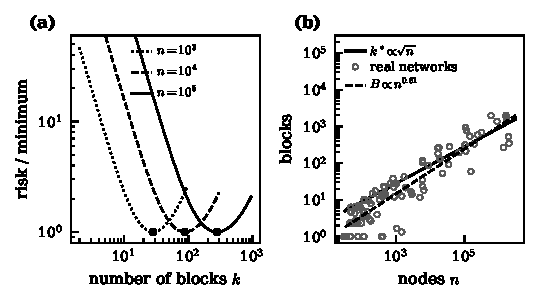
\includegraphics[width=\linewidth]{figs/fig-gr-resolution.pdf}
\caption{\textbf{How many blocks can be seen.} (a)~The risk of a $k$-block
description, Eq.~\eqref{eq:gr-risk}, for three network sizes, each normalized to
its own minimum (dots). The optimum moves right as $\sqrt{n}$. (b)~That optimum
against size, with the community counts of the real networks of the last chapter
and their fitted power law. The vertical placement of the $k^*$ line depends on
the graphon's smoothness constant and carries no meaning; its slope of one half
does.}
\label{fig:gr-resolution}
\end{figure}

And here the chapter's opening question returns, transformed. The $\sqrt{n}$ that
the last chapter used as its fractal yardstick --- the self-similar prediction of
$\sqrt{n}$ communities of $\sqrt{n}$ nodes --- turns out to be the same $\sqrt{n}$
that statistics arrives at from an entirely different direction, as the resolution
at which a smooth shape is best described. The book's models and the statisticians'
histograms agree on a number for reasons that have nothing to do with each other.

\section{Rough, not smooth}

Take the agreement seriously and the measured exponent stops being a curiosity and
becomes a measurement of something.

The real networks gave $\beta\approx0.61$, with a bootstrap interval
$[0.55,0.67]$ that excludes one half. Read through Eq.~\eqref{eq:gr-kstar}, an
exponent is no longer just a number above or below a fractal benchmark: it is a
statement about the smoothness of the shape being described. Inverting
$\beta=1/(1+\alpha)$,
\begin{equation}
  \alpha \;=\; \frac{1}{\beta}-1 \;\approx\; 0.65,
  \qquad \alpha\in[0.49,\,0.82],
  \label{eq:gr-alpha}
\end{equation}
and the interval lies wholly below $\alpha=1$. Direct minimization of
Eq.~\eqref{eq:gr-risk} at $\alpha=0.65$ returns an exponent of $0.611$, against
the measured $0.608$.

So the excess over $\sqrt{n}$ is not merely ``more communities than a fractal.''
It says that if real networks are converging to any limiting shape at all, that
shape is \emph{rough}: not Lipschitz, not smooth in the sense the estimation
theory assumes, but H\"older-continuous with an exponent around two thirds. A
smooth graphon --- any smooth graphon, of any shape, at any scale, since the
smoothness constant sets only the height of the line in
Figure~\ref{fig:gr-resolution}b and not its slope --- supports a description that
refines as $\sqrt{n}$ and no faster. Real networks refine faster than that. They
keep resolving new structure at every scale, at a rate a smooth limit cannot
supply.

This is the same conclusion the last chapter reached in its own language, and the
same one this book has been reaching since the introduction, arrived at from the
outside. A network built by a local rule has no smooth limiting shape to converge
to, because the rule keeps writing structure at whatever scale the network has
currently reached.

It is worth knowing that this is not a quarrel with the limit theory but an answer
to a question its own authors left open. Introducing a network generator built from
a singular measure rather than a function, \citet{palla2010} --- Lov\'asz among
them --- put the alternatives as plainly as they can be put:

\begin{quote}\small
Should we expect that large real graphs converge to some limiting network in a
strict sense of the convergence? Or, alternatively, their structure cannot be
mapped onto a fixed function, and only an ever-changing (with the size of the
network) measure (in the infinite network size limit becoming singular) can be used
to reflect the underlying structural complexity?
\end{quote}

\noindent That was posed in 2010 and left as a question. Equation~\eqref{eq:gr-alpha}
is a measurement bearing on it, taken across a hundred networks, and it comes down
on the second side: no fixed smooth function will do, because the description keeps
refining faster than any such function allows. The rest of this chapter is about how
far that answer can be trusted.

\section{Five meanings of one number}

A caution belongs here, and it is a sharp one. Five different arguments in this
book and its neighbouring literature all deliver $\sqrt{n}$, and they are not the
same statement:

\begin{itemize}
\item the \emph{fractal} $\sqrt{n}$ of the self-similar models --- a prediction
  about how many communities the networks themselves hold;
\item the \emph{geometric} $\sqrt{n}$ of Chapter~\ref{ch:distance} --- the
  multiplicity of shortest paths on the same lattice, a prediction about how many
  ways there are to cross it;
\item the \emph{constructive} $\sqrt{n}$ --- the resolution any cascade of equal
  cells is forced to, once its mean degree is held fixed;
\item the \emph{statistical} $\sqrt{n}$ of Eq.~\eqref{eq:gr-sqrtn} --- the best
  resolution obtainable for a smooth shape, a statement about descriptions;
\item the \emph{algorithmic} $\sqrt{n}$ --- the resolution limit of the
  non-nested block model, which cannot report more than of order $\sqrt{n}$
  groups no matter how many are present \citep{peixoto2014hier}.
\end{itemize}

The third of these is the one just met, and it is worth making explicit, because it
shows how little the number has to assume. Build a network from a singular measure
in the manner of \citet{palla2010}: divide the square into $m^2$ cells, give each a
probability, and multiply the whole pattern into itself $k$ times, so that the
picture has $m^k$ rows and grows sharper with every iteration. If the cells are all
the same size, the mean degree of the resulting network is $N m^{-2k}$, so holding
it fixed while refining the measure forces
\begin{equation}
  m^{k} \;=\; \sqrt{N/\langle k\rangle} \;\propto\; \sqrt{N} .
  \label{eq:gr-cascade}
\end{equation}
The construction resolves $\sqrt{N}$ rows because sparsity leaves it no choice. No
network, no estimator and no smoothness assumption enters that argument --- only
the bookkeeping of keeping a self-similar object sparse.

Three of the five now have reasons, and they are the same reason. The fractal and
geometric counts are a lattice's blocks and its routes tallied at the halfway point
of its own construction, and the constructive count is what any equal-celled cascade
must do to stay sparse; all three are self-similarity keeping its books. That is why
$\beta=1/2$ is the natural exponent for a self-similar object, and why measuring
$\beta>1/2$ says the object is not one --- the multifractal case, where the cells
are allowed to differ in size, has no such constraint and its exponent is free.
The remaining two agree with them for no reason at all.

The algorithmic $\sqrt{n}$ is a property of neither the network nor the ideal
description but of the instrument, and it deserves attention because the counts of
the last chapter were produced by exactly that instrument: a flat degree-corrected
block model selected by description length. Its ceiling and the null hypothesis under test
have the same functional form, which is an uncomfortable coincidence.

The bias runs in the reassuring direction --- a ceiling can only suppress the
counts of the largest networks and so pull the fitted exponent \emph{down},
meaning $\beta>1/2$ is measured in spite of the instrument rather than because of
it. But the conclusion that survives is correspondingly narrower: these data
establish an exponent above one half over four decades of size, and cannot by
themselves certify that it persists asymptotically, because the estimator that
produced them is not able to report an asymptotic exponent above one half. Only
the nested block model, which lifts the ceiling to order $n/\ln n$, can settle
that, and re-running the census with it is the obvious next measurement. Should
the exponent survive, Eq.~\eqref{eq:gr-alpha} converts it directly into a
statement about the roughness of the limit.

\section{What the ring cannot tell us}

One more thing the limit view clarifies, and it is a caveat about a result rather
than a strengthening of one.

The ring of the last chapter was found to prefer being split in two, for every
range $c\ge2$. But every node of the ring is identical to every other, and the
model was explicit that there is no preferred place to cut: rotate the proposed
partition by one bead and the evidence is unchanged. In the language of limits
that is a symmetry, and a continuous one. The ring's local limit --- what an
observer sitting on a node sees, out to any fixed distance
\citep{benjamini2001} --- is an infinite line, the same in every direction, with
no communities anywhere in it.

So the ring exhibits, in the cleanest possible form, a distinction the previous
chapter's machinery does not itself draw. Evidence for splitting is not the same
as the existence of a partition to be found. The ring supplies the first without
the second: a whole continuum of cuts, all equally good, none of them recoverable
from the data, and a limit object with no structure at all. What the evidence
ratio reports is that one block is a poor description --- a true and interesting
fact --- and not that two particular blocks are the right one. For the diamond
lattice and the pseudofractal web, whose partitions are pinned by their
construction, no such degeneracy arises and the identification is sound. It is the
homogeneous case that needs the care.

The ring is also the only one of the three entitled to that local limit, and the
reason is worth recording, because it marks out exactly where this book's networks
fall. A local limit of the kind just used requires an absolute ceiling on the
degree: every node must look like every other from close up, out to a bounded
number of neighbours. The ring obliges --- every node has degree $2c$ and always
will. The diamond lattice and the pseudofractal web do not: their poles grow
without bound, reaching degree $2^t$, so no ceiling exists and the local theory
does not apply to them. Nor does the theory at the other end, which needs the
number of links to outgrow the number of nodes, while theirs stays proportional
to it.

That is a genuine gap, and the book's central examples sit in it: too heavy-tailed
for the local theory, too sparse for the global one. It is also a gap the subject
knows about and is working to close --- a recent line of work \citep{backhausz2018}
proposes treating a network not as a picture at all but as an \emph{operator}, and
recovers dense graphons and local limits as two special cases of one notion of
convergence. Whether it reaches the case that matters here --- bounded mean degree
with unbounded hubs --- is precisely the question to put to it.

\section{What clustering rules out}
\label{sec:gr-clustering}

Everything so far has been about \emph{shape} --- whether a limiting picture
exists and how finely it can be resolved. There is a blunter test, and the
introduction ran it before any of this machinery was in place.

A graphon model, of any kind, draws its links independently once the positions of
the nodes are fixed. That is what makes it tractable, and it has a consequence
that cannot be argued away: a triangle needs three links, each drawn separately,
so triangles are as rare as three coincidences. In a sparse network the clustering
coefficient of such a model collapses to the link density itself, a number of
order $\langle k\rangle/n$ --- vanishing. Real networks are not like that, and the
introduction already measured by how much. Its column $C_{\mathrm{ER}}$, computed
there as the clustering of a random network of the same size and density, is
precisely the graphon prediction:

\begin{center}
\begin{tabular}{lccc}
\hline
Network & $C$ & $C_{\mathrm{ER}}$ & $C/C_{\mathrm{ER}}$ \\
\hline
Internet (AS)          & $0.230$  & $0.00018$ & $1254$ \\
Gnutella               & $0.0055$ & $0.000076$ & $72$ \\
Yeast proteins         & $0.071$  & $0.0018$  & $39$ \\
cond-mat co-authorship & $0.657$  & $0.00026$ & $2541$ \\
\hline
\end{tabular}
\end{center}

Between forty and two and a half thousand times too many triangles. No adjustment
of the shape $W$ repairs a discrepancy of that size, because the shape is not what
is wrong: the independence is.

But the argument has to be made carefully, and the careful version is more
interesting than the crude one. The comparison above is against a \emph{constant}
graphon, and we have already seen in
Section~\ref{sec:gr-blockmodel} that the constant is the weaker of the two
baselines. Against the \emph{rank-one} graphon --- the network reshuffled to
preserve every degree --- the verdict divides. The Internet's clustering falls only
from $0.230$ to $0.123$ under that reshuffling, a factor of $1.9$: its degrees
alone, hubs and all, manufacture most of its triangles, because a node of enormous
degree is shared by many pairs and closes their triangles by accident. The
co-authorship network, whose degrees are far less extreme, still stands $356$ times
above its own reshuffling.

So the two baselines separate the systems exactly as they separated the
pseudofractal's two cuts. Where the degrees are wild, degree heterogeneity accounts
for much of the clustering and little is left to explain. Where they are tame, the
whole of it survives the strongest degree-preserving null available --- and that
residue is what Chapter~\ref{ch:friends} was written to explain. Triadic closure is
not an embellishment on a graphon; it is the thing the graphon cannot do.

\section{Locality, or exchangeability}

There is a reason all of this bears on the book's thesis rather than merely
decorating it, and it is worth ending on.

A graphon is not only a limit; it is a complete description of a certain
\emph{kind} of random network --- those whose nodes are exchangeable, meaning the
labels carry no information and any two nodes are, before we look, the same
\citep{aldous1981,diaconis2008}. Every graphon model is exchangeable and every
exchangeable model is a graphon. Exchangeability is a strong assumption, and what
it excludes is precisely geometry: a node's position, its neighbourhood, its
history. It excludes locality.

The chapters before this one have argued that networks are built by nodes acting
on what is near them --- the page a surfer reached, the friend who made the
introduction, the gene that was copied. A rule of that kind produces a network in
which position matters, in which where a node attached is written into the
structure around it. Such a network is not exchangeable, and so it has no graphon
in the ordinary sense. The failure of the limit theory to say anything useful
about real networks, which began this chapter as an inconvenience, is at bottom
the same fact this book has been documenting all along, in a different vocabulary.
Sparsity and roughness and the absence of a smooth limit are what locality looks
like when a statistician goes looking for a shape.

What the sparse limits should be instead is an open and active question, and the
theory of sparse exchangeable graphs \citep{caron2017} is one serious attempt at
it. But it would be wrong to end by filing all of this under work not yet begun,
because on one point the previous chapter has already done a piece of it without
saying so.

The companion to the $L^p$ theory \citep{borgs2018} asks what it should
\emph{mean} for a sparse network to converge, and proves that several answers that
look quite different are the same answer. One can ask that the rescaled picture
settle down. One can ask that the \emph{quotients} settle --- the tables of
block-to-block densities produced by chopping the network into parts. One can ask
that the best partition at fixed block sizes settle, or that the sum over all such
partitions, weighted, settle: a ground state energy and a free energy, in the
language of physics. These are all equivalent.

That list is the last chapter's apparatus, item by item. A quotient is exactly the
table of counts $e_{rs}$ against expectations $\Omega_{rs}$. Fixed block sizes are
exactly the candidate split. The weighted sum over labelings, with the label prior
integrated out, is exactly the evidence. And the renormalization flow
$(u_{\mathrm{in}},u_\times)\to(K,0)$ is a quotient converging --- proved by hand,
for one lattice, in precisely the sense the theorem intends. That is why the
resulting $\ln K$ per link is so indifferent to the lattice that produced it:
convergence of quotients is a statement about the limiting shape, and any
arrangement with the same limiting quotient must give the same free energy.

The hypotheses of that theorem do not cover a bounded-degree lattice, so what the
last chapter proved is not a corollary of it; the flow had to be computed. But the
agreement of the two routes is worth more than either alone, and it marks out what
a limit theory for locally grown networks would have to look like. There is also,
on the other side of Eq.~\eqref{eq:gr-alpha}, a number measured across a hundred
real networks, still waiting to be explained.

\section{A conjecture, and two questions}
\label{sec:gr-conjecture}

The chapter has so far been an audit: what the limit theories can and cannot say
about networks grown by local rules. It ends with a programme instead, because the
audit points somewhere specific.

Start from what the last chapter actually did. It took networks grown by local
rules and \emph{fitted} them --- to a stochastic block model, by Bayesian
inference. A block model is a two-variable object, a kernel
$[0,1]^2\to[0,1]$ read through group labels, and the fit was good enough to
count communities across four decades of size. So a two-variable description
already captures something real. The question is what it misses, and whether the
miss has a shape.

There is a natural guess about that shape. A local rule does not act on pairs. Triadic
closure acts on \emph{triples} --- a node, its neighbour, and that neighbour's
neighbour --- and duplication acts on a node, its copy, and their shared
neighbours, a configuration of four. If the statistics a rule generates are to be
carried by a limiting object at all, the object may need arguments enough to hold
the rule's own footprint: a kernel $[0,1]^3\to[0,1]$ where the rule closes
triangles, $[0,1]^4\to[0,1]$ where it duplicates. This suggests a conjecture.

\begin{quote}
\emph{Conjecture.} For large $n$ the limit of a locally grown network is almost
equivalent to an exchangeable object --- but one of higher order than a graphon.
The order is set by the arity of the growth rule: three for triadic closure, four
for duplication, with the fitted block model as the two-variable shadow of it.
\end{quote}

\noindent The word \emph{almost} is carrying weight, and making it precise is part
of the problem. Two questions follow, and the first is answerable now.

\subsection*{Question 1: what does the fitted block model preserve?}

Given a network grown by a local rule and the block model that Bayesian inference
fits to it, which statistics agree and which do not? The honest answer has a clean
first instalment, and the pseudofractal web supplies it, because there every
quantity is exact.

\begin{calculation}{the triangles a two-variable model can hold}
The web has $n=(3^{t+1}+3)/2$ nodes and $3^{t+1}$ links, and every node added
closes exactly one triangle, so it holds exactly $n-2$ of them. Fit chapter~6's
branch cut and ask each fitted model how many it expects, via
$\mathrm{tr}(P^3)/6$ for its expected adjacency matrix $P$.

The plain block model assigns one density per block pair. In a sparse network
those densities fall like $1/n$, and a triple of blocks contributes
$n^3\times n^{-3}$: the expected count is $O(1)$, and numerically it
\emph{saturates} at $21.3$ triangles however large the web grows. Against a true
count rising like $n$, the deficit grows like $n$ itself.

The degree-corrected model does better, and still fails. Its expected count
weights each block by its squared-degree sum $Q_r=\sum_{i\in r}k_i^2$ rather than
by its size, and for this web $Q\sim4^{t}$ while the degree sum is $S\sim3^{t}$,
so the count grows as $(Q/S)^3\sim(64/27)^t$ against a truth growing as $3^t$. The
deficit again diverges, now as
\begin{equation}
  (81/64)^{t} \;=\; n^{\,0.214}.
  \label{eq:gr-tridef}
\end{equation}
Allowing the number of blocks to grow as the data demand, $B\propto n^{\beta}$,
helps but does not close it: $B$ blocks of $n/B$ nodes contribute $O(1)$ triangles
each, hence $n^{\beta}$ in all, still short of $\Theta(n)$ by $n^{1-\beta}$.
\end{calculation}

So the answer to the first question, for this network, is sharp. A two-variable
description preserves what the cut metric sees --- block densities, degrees, the
evidence for a partition, everything the last chapter computed --- and loses the
3-point structure entirely, by a margin that widens without bound. Even a
hierarchy of blocks, refining as fast as real networks demand, recovers only
$n^{\beta}$ of the $n$ triangles.

One warning for anyone testing this at accessible sizes: the failure is not
visible early, and it changes sign. At $n\simeq3000$ the degree-corrected model
\emph{over}counts triangles fivefold, and only past $n\sim10^8$ does it cross over
to undercounting. A study stopping at ten thousand nodes would conclude the
opposite of the truth.

\subsection*{Question 2: does higher order close the gap?}

If two variables are not enough, are three? Here the conjecture meets a genuine
obstacle, and the obstacle locates exactly where its content lies.

For \emph{dense} graphs the question is already settled, and settled against the
conjecture. An exchangeable array admits the representation
$f(\xi_\emptyset,\xi_i,\xi_j,\xi_{ij})$, and for a simple dense graph the
pair-level variable $\xi_{ij}$ can always be absorbed into a threshold, leaving a
two-variable kernel. Exchangeability \emph{forces} the graphon form; no
higher-order object can add anything. Whatever the conjecture is claiming, it
cannot be claiming that.

Its content therefore lies entirely in the sparse regime --- which is the regime
this whole chapter has been about, and the reason the clustering of
Section~\ref{sec:gr-clustering} does not vanish when a graphon says it must. There,
the pair-level randomness does not wash out, and the natural object keeps
arguments indexed by \emph{pairs} rather than by nodes: not $W(x_i,x_j,x_k)$ but
something closer to $W(x_{ij},x_{ik},x_{jk})$, which is the shape the limit theory
of hypergraphs already takes. That is a refinement of the conjecture rather than a
refutation of it, and it says where to look: triadic closure makes the presence of
one link depend on two others sharing a node, and a pair-indexed kernel is the
smallest object that can express such a dependence.

\subsection*{The same failure, with the arity changed}

The diamond lattice tests whether any of this was about triangles. It cannot be:
the lattice is bipartite and contains no triangle at all. Its rule replaces each
link with two parallel paths, so the motif it manufactures is the \emph{four}-cycle,
and the same question can be put again with the arity moved by one.

\begin{calculation}{the four-cycles a two-variable model can hold}
After $t$ generations the lattice has $m=4^t$ links and $n=(2\cdot4^t+4)/3$ nodes.
Only the diamonds closed at the \emph{last} generation are still four-cycles ---
earlier ones have had their links subdivided into longer loops --- so the count is
exactly $4^{t-1}$, again proportional to $n$. Fitting chapter~6's cut into two
branches and evaluating $\mathrm{tr}(P^4)/8$:

The plain block model saturates, as before, and here the constant can be named. In
the limit the two blocks are near-independent, each of $n_r\simeq4^t/3$ nodes at
density $p\simeq9/4^{t}$, contributing $n_r^4p^4/8=81/8$ four-cycles apiece:
\begin{equation}
  \text{plain model} \;\longrightarrow\; \tfrac{81}{4} = 20.25
  \label{eq:gr-quadsat}
\end{equation}
four-cycles, for a lattice of any size.

The degree-corrected model is where the two lattices part company. Its count is
governed by the ratio of the squared-degree sum to the degree sum, and for this
lattice that ratio is not a power of $n$ at all but
\begin{equation}
  Q/S \;=\; \sum_i k_i^2 \Big/ \sum_i k_i \;=\; t+1
  \label{eq:gr-QS}
\end{equation}
exactly, so the expected four-cycle count converges to $(t+1)^4/4$: \emph{poly\-log\-arithmic}
in $n$, against a truth growing as $n/6$. At $t=26$ the lattice holds
$1.1\times10^{15}$ four-cycles and the fitted degree-corrected model expects
$1.3\times10^{5}$ of them.
\end{calculation}

That gap --- a factor of $n/(\ln n)^4$ --- is far worse than the pseudofractal's
$n^{0.214}$, and the reason is the one thing the two lattices genuinely differ in.
The pseudofractal's degrees are wild, $\gamma\simeq2.585$, and a rank-one model
with hubs that extreme manufactures a great many triangles by accident: three
links that all happen to touch the same few enormous nodes close a triangle
whether or not any rule intended it. The diamond's degrees are milder,
$\gamma=3$ exactly, which is the marginal case where $\sum k_i^2$ outgrows
$\sum k_i$ only logarithmically --- and a rank-one model then has nothing to fake
with.

So the two-variable model's apparent grasp of higher-order structure is not a grasp
at all. It is borrowed entirely from degree heterogeneity, and it fails as the
degrees become tame. That is a mechanism for something already measured in
Section~\ref{sec:gr-clustering}: there the degree-preserving null came within a
factor of $1.9$ of the Internet's clustering, whose degrees are extreme, and fell
$356$ times short for co-authorship, whose degrees are not. The deterministic
lattices say why, and warn against the natural misreading --- that degree-corrected
models capture clustering. They capture it exactly where the degrees are heavy
enough to counterfeit it.

\subsection*{The whole spectrum at once}

Triangles and four-cycles are two points. Asking the question at every cycle
length turns the finding from a shortfall into something more damaging.

\begin{calculation}{why a two-variable model has a one-parameter spectrum}
For a model with independent links and expected adjacency $P$, the expected number
of $L$-cycles is $\mathrm{tr}(P^L)/2L$. When $P$ is a $K$-block fit this collapses
onto a $K\times K$ \emph{transfer matrix}
\begin{equation}
  T_{rs} \;=\; \omega_{rs}\sqrt{Q_rQ_s}
  \qquad\text{(degree-corrected)},
  \label{eq:gr-transfer}
\end{equation}
with $Q_r=\sum_{i\in r}k_i^2$, and $T_{rs}=p_{rs}\sqrt{n_rn_s}$ for the plain
model, so that the count at every length is $\mathrm{tr}(T^L)/2L$. The entire motif
spectrum is generated by one small matrix, and for large $L$ it is
$\lambda^L/2L$ for the leading eigenvalue $\lambda$ --- a smooth geometric profile.
A two-variable model has no freedom to put a feature at one particular length,
whatever its blocks are doing.
\end{calculation}

The lattices do nothing but put features at particular lengths. The diamond is
built from four-cycles and carries cycles of length $4$, $8$, $16$, and so on ---
and \emph{exactly none} at any other length. Counted directly at $t=5$: zero
$3$-cycles, $256$ four-cycles, zero at five, six and seven, $1024$ eight-cycles.
The fitted models, meanwhile, expect $8.3$ triangles, $42$ five-cycles and $104$
six-cycles under the plain fit, and $69$, $1560$ and $8171$ under the
degree-corrected one, at lengths where the lattice contains nothing whatever.

So the failure is not that the numbers are too small. It is that a two-variable
model places mass at every length while a locally grown lattice places it at a
few, and no adjustment of blocks or degrees can move a smooth profile onto a
sparse set of lengths. This is a stronger statement than the triangle deficit, and
it is the one that argues for the conjecture: what a higher-order object buys is
not a bigger number but the ability to have a shape.

The pseudofractal makes the same point from the other side. Its degree-corrected
fit does not merely undercount; it \emph{changes sign} along the spectrum,
running short at $L=3$ and then overshooting ever more wildly --- by a factor of
$20$ at $L=5$ and $10^4$ at $L=8$. The reason is now visible in
Eq.~\eqref{eq:gr-transfer}: the leading eigenvalue of a degree-corrected fit is
essentially $\langle k^2\rangle/\langle k\rangle$, so its spectrum grows like
that ratio raised to the length, and for a degree distribution $p(k)\sim
k^{-\gamma}$,
\begin{equation}
  \lambda \;\sim\; n^{(3-\gamma)/(\gamma-1)} \quad (\gamma<3), \qquad
  \lambda \sim \ln n \quad (\gamma=3).
  \label{eq:gr-lambda}
\end{equation}
For the pseudofractal, $\gamma\simeq2.585$ gives the exponent $0.2619$, which is
exactly the growth its transfer matrix shows; for the diamond, $\gamma=3$ gives
the logarithm and $Q/S=t+1$. One quantity therefore governs both earlier results:
the deficit at length $L$ is of order $n/\lambda^{L}$, undercounting while
$\lambda^L<n$ and overcounting after. The rank-one part does not describe
higher-order structure at any length. It manufactures a geometric series and
happens to cross the truth once.

Two things would move this further. On the deterministic side the crossing point
is a prediction to test: Eq.~\eqref{eq:gr-lambda} says it sits at
$L^\ast=(\gamma-1)/(3-\gamma)$, which is near $4$ for the pseudofractal and
recedes to infinity as $\gamma\to3$. On the real networks the deficit is
measurable directly --- fit the block model, sample from the fit, and compare motif
counts with the original. If the conjecture holds, the gap should close as the
order of the fitted object rises to the arity of the rule that built the network,
and stop closing thereafter.


\chapter{Communities with network motifs}
\label{ch:motifs}

The last chapter asked how finely a network can be divided, and answered it with
two priors over the same object. This one asks a different question: what the
divider is allowed to \emph{know} about the thing it is dividing.

Start with cycles, because they are where a network's local structure shows
itself. Every network has cycles of every length, and their numbers are not
remotely comparable: the yeast interactome holds a couple of hundred triangles
and ten thousand cycles of length eight, and a duplication--divergence network of
two hundred nodes holds none of length three, five or seven and seven million of
length eight. The counts climb steeply with length, and the steepness is not a
free parameter --- it is set by the short cycles.

That is the fact this chapter is built on, and it is worth stating at the outset.
The number of $h$-cycles through a node of degree $k$ is fixed by the degree
distribution together with one three-point quantity, the clustering coefficient,
and the length enters only as an exponent: the same closing probability applied
$h-2$ times around the loop (Section~\ref{sec:gr-conjecture}). Long cycles are not an
independent feature of a network. They are what short cycles compound into. A
description that has the triangles right has the whole spectrum right, wherever
triangles exist at all.

Wherever they do not, the compounding starts from something else, and the
question of \emph{which} something else turns out to be answerable by
measurement. A rule that closes squares rather than triangles leaves a spectrum
with a different shape, and one that closes pentagons a different shape again.

All of which bears on communities in a way that is not obvious until it is
stated. A block model divides a network on the evidence of where its links fall.
Clustering is evidence: a knot of mutually connected nodes looks like a
community. But if the network was grown by a rule that closes triangles
everywhere, the knots are not communities at all, and a method that could
\emph{name} a triangle would have an innocent explanation available where a
method without one has only the partition. So the question of this chapter is
whether giving a community model a vocabulary of motifs changes what it reports.
The answer, worked out over the sections that follow, is that it usually changes
when communities appear and not how many there are --- but that on two rules out
of eight it does something larger, and moves the network into a different limit
class altogether.

The concern is not new, and neither is the vocabulary. Recurring small subgraphs
were named \emph{network motifs} by \citet{milo2002}, who found them at
frequencies no random graph with the same degrees would produce; random graph
ensembles built to contain prescribed subgraphs rather than prescribed links were
constructed by \citet{karrer2010subgraphs}, and the model of
Section~\ref{sec:gr-motifsbm} is a block-structured version of theirs. Closest of
all, \citet{peixoto2022triadic} put exactly the suspicion above to work: a block
model in which each link is generated either by community membership or by
triadic closure over an existing path, with the assignment inferred alongside the
partition. On real networks it removes a good deal of what a plain block model
had been calling community structure. What follows differs in two ways. The
alphabet is not fixed to the triangle --- squares and bicliques are in it too,
because Chapter~\ref{ch:duplication}'s rules do not close triangles --- and the
target is not any one network but the \emph{scaling}, how the number of
communities grows with size and whether that exponent is a property of the
network or of the vocabulary used to describe it.

\section{Why a few motifs might be enough}
\label{sec:gr-conjecture}

Chapter~\ref{ch:graphons} ended by conjecturing that a locally grown network
converges to no kernel on the unit square at all, of two arguments or of any
number, and that what characterises its limit is instead intensive: a density of
communities, constant in size and set by the rule. It reached that conclusion by
abandoning an earlier guess --- that the limit is a kernel of \emph{higher
arity}, three arguments where the rule closes triangles and four where it
duplicates, with the fitted block model as the two-variable shadow of it.

This section takes the abandoned guess seriously for as long as it is useful,
which is not all the way. Its purpose is not to settle what the limit object is;
that question is left where Chapter~\ref{ch:graphons} left it. Its purpose is to
license an instrument. If a two-variable description can be shown to lose
something with a definite shape, and the shape can be shown to be fixed by the
shortest cycle the rule closes, then the way to build a better community model is
not to raise the arity of everything --- which is unaffordable, as we shall see
--- but to hand the ordinary pair model a small vocabulary of short motifs. That
is the conjecture this section exists to state. Everything after it is a test of
the instrument, not of the conjecture.

\subsection*{What a two-variable fit loses}

Take the two lattices whose construction is known exactly, so that every quantity
can be computed rather than estimated.

\begin{calculation}{the higher-order structure a two-variable model can hold}
The pseudofractal web of \citet{dorogovtsevgoltsev2002} has $n=(3^{t+1}+3)/2$
nodes and $3^{t+1}$ links, and every node added closes exactly one triangle, so
it holds exactly $n-2$ of them. Fit Chapter~\ref{ch:communities}'s branch cut and
ask each fitted model how many it expects, via $\mathrm{tr}(P^3)/6$ for its
expected adjacency matrix $P$.

The plain block model assigns one density per block pair. In a sparse network
those densities fall like $1/n$, and a triple of blocks contributes
$n^3\times n^{-3}$: the expected count is $O(1)$, and numerically it
\emph{saturates} at $21.3$ triangles however large the web grows.

The degree-corrected model does better, and still fails. Its expected count
weights each block by the degree sum $Q_r=\sum_{i\in r}k_i(k_i-1)$ rather than by
its size --- $k(k-1)$ and not $k^2$, because a triangle leaves a node by a
different link than it entered by, and the fit holds the degrees fixed --- and
for this web $Q\sim4^{t}$ while the degree sum is $S\sim3^{t}$, so the count
grows as $(Q/S)^3\sim(64/27)^t$ against a truth growing as $3^t$. The deficit
diverges, as $(81/64)^{t}=n^{0.214}$. Allowing the number of blocks to grow as
the data demand, $B\propto n^{\beta}$, helps but does not close it: $B$ blocks of
$n/B$ nodes contribute $O(1)$ triangles each, hence $n^{\beta}$ in all, still
short of $\Theta(n)$ by $n^{1-\beta}$.

The diamond lattice moves the arity by one and makes the failure worse. It is
bipartite and holds no triangle at all; its rule replaces each link with two
parallel paths, so its motif is the four-cycle, and after $t$ generations it has
$m=4^t$ links, $n=(2\cdot4^t+4)/3$ nodes and exactly $4^{t-1}$ four-cycles ---
only those closed at the \emph{last} generation are still four-cycles, earlier
ones having had their links subdivided into longer loops. Evaluating
$\mathrm{tr}(P^4)/8$ on the same cut, the plain model again saturates, at
$81/4=20.25$ four-cycles for a lattice of any size. The degree-corrected model is
where the two lattices part company: its count is governed by the ratio of the
excess-degree sum to the degree sum, and for this lattice that ratio is not a
power of $n$ at all but
\begin{equation}
  Q/S \;=\; \sum_i k_i(k_i-1) \Big/ \sum_i k_i \;=\; t
  \label{eq:gr-QS}
\end{equation}
exactly, so the expected four-cycle count converges to $t^4/4$:
\emph{poly\-log\-arithmic} in $n$, against a truth growing as $n/6$. At $t=26$ the
lattice holds $1.1\times10^{15}$ four-cycles and the fitted degree-corrected
model expects $1.2\times10^{5}$ of them.
\end{calculation}

So a two-variable description preserves what the \emph{cut metric} sees --- the
yardstick the limit theory uses, which judges two networks close when no way of
splitting the nodes into two sets reveals a difference in the density of links
across the split, and so registers block densities, degrees, the evidence for a
partition, everything Chapter~\ref{ch:graphons} computed --- and loses the
higher-order structure entirely, by a margin that widens without bound.

The gap between the two lattices --- $n^{0.214}$ against $n/(\ln n)^4$ --- is the
one thing they genuinely differ in, and it is worth naming because it recurs. The
pseudofractal's degrees are wild, $\gamma\simeq2.585$, and a rank-one model with
hubs that extreme manufactures a great many triangles by accident: three links
that all happen to touch the same few enormous nodes close a triangle whether or
not any rule intended it. The diamond's degrees are milder, $\gamma=3$ exactly,
which is the marginal case where $\sum k_i^2$ outgrows $\sum k_i$ only
logarithmically --- and a rank-one model then has nothing to fake with. The
two-variable model's apparent grasp of higher-order structure is not a grasp at
all; it is borrowed from degree heterogeneity, and it fails as the degrees become
tame. That is the mechanism behind something already measured in
Section~\ref{sec:gr-clustering}, where the degree-preserving null came within a
factor of $1.9$ of the Internet's clustering, whose degrees are extreme, and fell
$356$ times short for co-authorship, whose degrees are not. Degree-corrected
models do not capture clustering. They capture it exactly where the degrees are
heavy enough to counterfeit it.

One warning for anyone testing this at accessible sizes: the failure is not
visible early, and it changes sign. At $n\simeq3000$ the degree-corrected model
\emph{over}counts triangles fivefold, and only past $n\sim10^8$ does it cross
over to undercounting. A study stopping at ten thousand nodes would conclude the
opposite of the truth.

\subsection*{What is lost has a shape}

Triangles and four-cycles are two points. Asking the question at every cycle
length turns the finding from a shortfall into something with more content ---
and it is the content that motivates the alphabet.

\begin{calculation}{why a two-variable model has a one-parameter spectrum}
For a model with independent links and expected adjacency $P$, the expected number
of $L$-cycles is $\mathrm{tr}(P^L)/2L$. When $P$ is a $K$-block fit this collapses
onto a $K\times K$ \emph{transfer matrix}
\begin{equation}
  T_{rs} \;=\; \omega_{rs}\sqrt{Q_rQ_s}
  \qquad\text{(degree-corrected)},
  \label{eq:gr-transfer}
\end{equation}
with $Q_r=\sum_{i\in r}k_i(k_i-1)$, and $T_{rs}=p_{rs}\sqrt{n_rn_s}$ for the plain
model, so that the count at every length is $\mathrm{tr}(T^L)/2L$. The entire motif
spectrum is generated by one small matrix, and for large $L$ it is
$\lambda^L/2L$ for the leading eigenvalue $\lambda$ --- a smooth geometric profile.
A two-variable model has no freedom to put a feature at one particular length,
whatever its blocks are doing.

The weight is $k(k-1)$ rather than $k^2$ because a cycle leaves a node by a
different link than the one it arrived on, and the degree-corrected fit holds the
degree sequence fixed: a node offers $k(k-1)$ ordered pairs of links, not $k^2$.
The one-block case is then $\langle k^2-k\rangle/\langle k\rangle$, which is the
leading eigenvalue of the \emph{non-backtracking} operator, which counts walks
forbidden to turn round and retrace the link they arrived on --- the natural
object for cycles, since a cycle never does. The distinction is invisible in the
limits taken above, where the ratio diverges and the $-1$ is lost, but it is
worth a factor of $25$ at $L=8$ on a real network, where the ratio is nearer $3$.
\end{calculation}

The lattices do nothing but put features at particular lengths. The diamond is
built from four-cycles and carries cycles of length $4$, $8$, $16$, and so on ---
and \emph{exactly none} at any other length. Counted directly at $t=5$: zero
$3$-cycles, $256$ four-cycles, zero at five, six and seven, $1024$ eight-cycles.
The fitted models, meanwhile, expect $8.3$ triangles, $42$ five-cycles and $104$
six-cycles under the plain fit, and $40$, $668$ and $2994$ under the
degree-corrected one, at lengths where the lattice contains nothing whatever.

So the failure is not that the numbers are too small. It is that a two-variable
model places mass at every length while a locally grown lattice places it at a
few, and no adjustment of blocks or degrees can move a smooth profile onto a
sparse set of lengths. What a richer description buys is not a bigger number but
the ability to have a shape --- and a \emph{shape} supported on a few short
lengths is exactly what a small alphabet of motifs is.

That the shape is generated by one eigenvalue also fixes how the two lattices
differ. For a degree distribution $p(k)\sim k^{-\gamma}$,
\begin{equation}
  \lambda \;\sim\; n^{(3-\gamma)/(\gamma-1)} \quad (\gamma<3), \qquad
  \lambda \sim \ln n \quad (\gamma=3),
  \label{eq:gr-lambda}
\end{equation}
which gives the pseudofractal's exponent $0.2619$ and the diamond's $Q/S=t$. One
quantity governs both earlier results: the deficit at length $L$ is of order
$n/\lambda^{L}$, undercounting while $\lambda^L<n$ and overcounting after. The
rank-one part does not describe higher-order structure at any length. It
manufactures a geometric series and happens to cross the truth once.

That crossing is a falsifiable prediction, and it was tested on $44$ real
networks, with cycles counted exactly at $L=3\ldots8$ and each fitted model
represented by a sample from it rather than by the formula. Half of it came back
confirmed, and it is the half the argument stands on: a fitted model's own motif
spectrum really is generated by its transfer matrix, the sampled counts sitting
on $\lambda^L/2L$ to within one per cent at every length
(Figure~\ref{fig:gr-crossover}a). Eq.~\eqref{eq:gr-transfer} is not an
approximation that degrades. The crossing itself does not survive: real networks
carry many more cycles than their rewirings at \emph{every} length alike --- five
times more at the median, four thousand times for a large co-purchase network ---
and the excess barely decays, the measured slope being about a tenth of
$-\ln\lambda$, with thirty-nine of forty-two networks departing from the
predicted slope by more than two standard errors
(Figure~\ref{fig:gr-crossover}b). The deficit is a level, not a slope. The
lattices' motif counts are extensive and flat in $L$, so dividing by a geometric
profile leaves a geometric deficit and a crossing; real networks' cycle counts
grow with $L$ at very nearly the rate their rewirings do. The crossing is a
property of the deterministic webs, and the $L^\ast$ formula should be read as a
statement about them.

\begin{figure}[t]
  \centering
  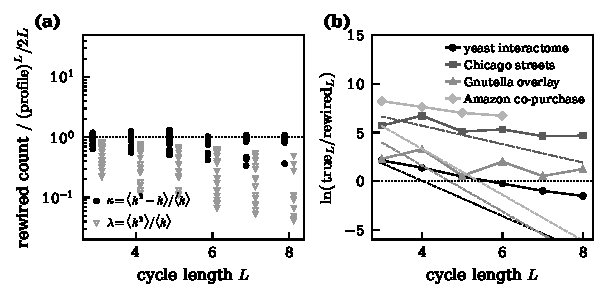
\includegraphics[width=\linewidth]{figs/fig-gr-crossover.pdf}
  \caption{The two halves of the prediction, on real networks. \textbf{(a)} A
  degree-preserving rewiring's own cycle counts, divided by the geometric profile
  its transfer matrix predicts. With the excess-degree branching factor
  $\langle k^2-k\rangle/\langle k\rangle$ the ratio sits on $1$ at every length;
  with $\langle k^2\rangle/\langle k\rangle$ it drifts away by an order of
  magnitude. \textbf{(b)} The deficit $\ln(\text{true}_L/\text{rewired}_L)$ for
  four systems, against the line of slope $-\ln\lambda$ through
  $L^\ast=\ln n/\ln\lambda$ that Eq.~\eqref{eq:gr-lambda} predicts (dashed). The
  measured curves are large and nearly flat.}
  \label{fig:gr-crossover}
\end{figure}

None of that touches the support argument, which the same measurement instead
strengthened by turning up a real network with the diamond's pathology.
Fullerenes are molecules, and their cycle spectra are exactly $12$ five-cycles
and $n/2-10$ six-cycles and \emph{nothing at any other length} --- twelve
pentagons at every size, which is Euler's theorem. Both fitted models put
positive mass everywhere: for $\mathrm{C}_{6000}$, five triangles, forty-three
four-cycles, twenty-seven seven-cycles. There the deficit is not fivefold or four
thousandfold, it is infinite in both directions, and no choice of blocks or
degrees can repair it.

\subsection*{How short a vocabulary has to be}

The shape is supported on a few lengths. How few, and which, is not something to
be postulated, because the cycle spectrum of a real network is already known to
be generated by a local quantity of arity three. Write $p_k$ for the degree
distribution and $c_k$ for the clustering coefficient of a node of degree $k$.
Then the number of $h$-cycles through a node of that degree
is~\citep{vazquez2005cycles}
\begin{equation}
  \frac{N_h}{n} \;=\; g_h\sum_{k}p_k\,\frac{(h-1)!}{2}\binom{k}{h-1}\,c_k^{\,h-2},
  \label{eq:gr-cycgen}
\end{equation}
with $g_h$ a correction for multiple counting: choose $h-1$ neighbours of a
central node, order them, and close the cycle by requiring $h-2$ links among
consecutive ones, each present with probability $c_k$. The degree distribution
and one three-point quantity fix the count at \emph{every} length, and the
measurement holds at $h=3,4,5$ across co-authorship, the Internet and a semantic
network~\citep{vazquez2005cycles}.

This is the licence the alphabet needs. The tower of longer cycles requires no
mechanism of its own: it is the product $c_k^{\,h-2}$, the same closing
probability applied $h-2$ times around the loop. Arity three buys not just the
triangle but the whole spectrum built from triangles, and for a great many real
networks triangles do the job.

They cannot do it for a network with no triangles. There $c_k=0$ identically,
Eq.~\eqref{eq:gr-cycgen} vanishes at every $h\ge3$, and the failure is not an
underestimate but an empty prediction --- against a network full of cycles. The
book's own duplication--split rule is exactly that case, built so that
duplication makes no triangles and splitting destroys any that might form.
Counting $DS(n,1/3)$ directly at $n=2000$: no triangles at all, then
$1.1\times10^4$ squares, $7.9\times10^3$ five-cycles and $1.3\times10^7$
eight-cycles. Nothing about the network is short of cycles; the arity-three
generator simply cannot see any of them.

So the order required is set by the shortest cycle the rule closes, and it is
measurable rather than postulated. The bubble family makes it a dial, since
$BB(n,L)$ closes a fresh cycle of length $L+2$ at every step:

\begin{center}
\begin{tabular}{llll}
\hline
model & motif & $c$ & cycle lengths present, $L=3\ldots10$\\
\hline
$BB(n,1)$ & triangle & $0.74$ & every length\\
$BB(n,2)$ & square & $0$ & $4,6,8,10$\\
$BB(n,3)$ & pentagon & $0$ & $5,8$\\
$BB(n,4)$ & hexagon & $0$ & $6,10$\\
\hline
\end{tabular}
\end{center}

\noindent Only the first is within reach of Eq.~\eqref{eq:gr-cycgen}. The others
place their mass exactly where the motif and its gluings put it: two faces
sharing a link close a cycle of length $a+b-2$, so pentagons give $5$ and $8$,
hexagons $6$ and $10$, and everything else is empty. That is the same arithmetic
the fullerenes obey --- twelve pentagons and $n/2-10$ hexagons at any size, then
$60$ nine-cycles and $3n/2-60$ ten-cycles, with seven and eight empty because no
two pentagons touch. A molecule and a growth rule, agreeing on a rule about which
templates may be adjacent.

\subsection*{The conjecture, and why not a tensor}

Three things have now been established, and together they say what to build. A
two-variable fit loses the higher-order structure by a diverging margin. What it
loses is not a number but a shape, supported on a few short lengths. And which
lengths are populated is fixed by the shortest cycle the rule closes, everything
longer following from it by compounding. Hence:

\begin{quote}
\emph{Conjecture.} A small alphabet --- the link, the triangle, the square, and
whatever else a rule's own footprint requires --- is sufficient vocabulary for
describing a locally grown network. Naming the shortest cycle a rule closes
accounts for the higher-order structure a two-variable model loses, and no
higher-arity object is needed to hold it.
\end{quote}

\noindent The alternative is to raise the arity of the model itself, and it is
worth saying why that is not done here. In the dense case the question is already
settled against it: an exchangeable array admits the representation
$f(\xi_\emptyset,\xi_i,\xi_j,\xi_{ij})$, and for a simple dense graph the
pair-level variable $\xi_{ij}$ can always be absorbed into a threshold, leaving a
two-variable kernel. Exchangeability \emph{forces} the graphon form; no
higher-order object can add anything. Whatever raising the arity buys, it cannot
be that, and its content lies entirely in the sparse regime --- which is the
regime this whole book is about, and the reason the clustering of
Section~\ref{sec:gr-clustering} does not vanish when a graphon says it must.
There the pair-level randomness does not wash out, and the natural object keeps
arguments indexed by \emph{pairs} rather than by nodes: not $W(x_i,x_j,x_k)$ but
something closer to $W(x_{ij},x_{ik},x_{jk})$, which is the shape the limit
theory of hypergraphs already takes. The inferential side of that idea has been
built: \citet{young2021hypergraph} ask, of an ordinary pairwise network, which of
its cliques are better explained as single higher-order interactions than as the
links they appear to be, and answer by description length. It is the same
accounting used below, with hyperlinks in place of motifs.

In practice, though, the tensor is unaffordable, and Chapter~\ref{ch:graphons}
priced it exactly: a block model over $j$-sets has a count tensor with about
$B^j/j!$ entries, and balancing that against what a split saves gives
$B_{\max}\approx[m(j-1)!/\ln m]^{1/j}$, which is $\sqrt n$ at $j=2$ and $n^{1/4}$
at $j=4$ --- eighteen groups where the pair model recovers three hundred and
sixteen (Eq.~\eqref{eq:gr-bmax}). A model that can no longer see communities is a
poor instrument for asking what communities are made of. The conjecture's virtue
is that it buys the shape without paying that price, and the next section builds
the instrument that follows from it.

\section{Fitting the order, not assuming it}
\label{sec:gr-motifsbm}

All of that still asks the reader to accept the arity of each rule as given. It
can instead be \emph{inferred}, by the same criterion that fits a block model in
the first place: minimum description length. The posterior of
Section~\ref{sec:gr-blockmodel} is \emph{microcanonical} --- it fixes the link
counts exactly rather than only on average, so that a model is a set of
constraints and the description length counts the networks satisfying them --- and
$\Sigma=-\log_2P(A,e,b)$ makes no use of the fact that links join two nodes. Nothing stops us handing it a
model built from something else.

\begin{calculation}{an alphabet of motifs, priced}
The obvious something else --- a block model over $4$-sets, its count matrix
replaced by a four-index tensor --- is the wrong choice, and
Section~\ref{sec:gr-twopriors} has already priced it: a $j$-index tensor drops the
resolution to $B_{\max}\approx[m(j-1)!/\ln m]^{1/j}$, which at $j=4$ is $n^{1/4}$,
eighteen groups where the pair model recovers three hundred and sixteen. A model
that can no longer see communities is a poor instrument for asking what
communities are made of.

The affordable object keeps the ordinary block structure and changes what the
blocks are built from. Every link is assigned to exactly one \emph{motif
instance} drawn from a small alphabet --- a link, a triangle, a square --- with
motifs of arity three and above planted inside a single block, and instances
wired by \emph{stub matching}: each node is given a number of loose link-ends,
or stubs, and the ends are then paired off at random, so that a node's share of
the motifs is fixed by how many stubs it was given. That generative recipe is
\citeauthor{karrer2010subgraphs}'s subgraph configuration model
\citeyearpar{karrer2010subgraphs}, run inside blocks. Planting $c$
copies of a motif that spans $s$ nodes inside one block can be done in
\begin{equation}
  \Omega \;=\; \frac{(sc)!}{\prod_i d_i!\;c!\;a^{c}}
  \label{eq:gr-omega}
\end{equation}
ways, where $d_i$ is how many of them node $i$ takes part in and $a$ is the size
of the motif's automorphism group --- the number of relabellings of its own nodes
that leave it unchanged, which is $2$ for a link, $6$ for a triangle and $8$ for
a square. Dividing by $a^{c}$ is what stops the same motif being counted once for
each way of writing it down. $\Sigma$ is then the sum of $\log_2\Omega$ over the
blocks together with the cost of the partition and of the counts. The parameters
number one count per motif type per block plus the block matrix, $3B+B^2$ for the
alphabet used here, rather than the $B^4/24$ of the tensor, so the
resolution ceiling stays at Eq.~\eqref{eq:gr-flatceiling}'s. The price is that a triangle straddling
two blocks is not representable and is described as three links instead.
\end{calculation}

Two features make this a test rather than a fitting exercise. With the alphabet
reduced to the link alone, $\Sigma$ is exactly the description length of the
ordinary degree-corrected model, so enlarging the alphabet is a strictly nested
comparison and a negative $\Delta\Sigma$ means the motifs paid for themselves. And
the criterion can tell a planted triangle from three incidental links, because
$c$ planted triangles are more constrained --- hence cheaper to specify --- than
the $3c$ independent links they account for, while the extra counts cost only a
little. Where triangles are unavoidable rather than planted the arithmetic goes
the other way, and on a nine-node graph carrying $26$ of its $36$ possible links
the criterion correctly plants none at all.

Run against the networks whose construction is known exactly, it recovers the
rule:

\begin{center}
\begin{tabular}{lrrl}
\hline
network & $n$ & $\Delta\Sigma$ (bits) & selected\\
\hline
pseudofractal, $t=5$      & 366 & $-398$ & triangle\\
$BB(n,1)$                 & 500 & $-259$ & triangle\\
diamond, $t=5$            & 684 & $-1032$ & square\\
$DS(n,1/3)$               & 500 & $-39$  & square\\
$BB(n,2)$                 & 500 & $-204$ & square\\
$BB(n,3)$, pentagons      & 500 & $+21$  & none\\
$BB(n,4)$, hexagons       & 502 & $+19$  & none\\
fullerene $\mathrm{C}_{240}$ & 240 & $+17$ & none\\
\hline
\end{tabular}
\end{center}

\noindent The last three rows are the ones that matter. Their motifs lie outside
the alphabet, and there the enlarged model costs bits and buys nothing --- the
$+17$ is precisely the price of announcing two totals that turn out to be zero.
It does not offer a square when the network was built from pentagons. A planted
network with triangles in one community and squares in another is recovered with
both, each in its own block; and the diamond at $t=4$ is decomposed into exactly
$64=4^{t-1}$ squares, the number it actually contains.

Two cautions. The decomposition assigns each link to one instance, so motifs that
overlap cannot all be represented: the pseudofractal holds $n-2$ triangles but at
most a third of its links' worth are disjoint, and $138$ were found. The
selection is meaningful; the counts are not estimates. And the search is greedy
in two coupled directions at once, which can trap it --- on the diamond, the
branch cut of Chapter~\ref{ch:communities} places \emph{every} four-cycle across
the cut, so from that partition the model finds no motif at all, and only a
different starting partition reveals them.

So the conjecture of Section~\ref{sec:gr-conjecture} holds up as far as the
instrument can be checked against networks whose construction is known. A symbol
of arity three pays for itself where the rule closes triangles, one of arity four
where it closes squares, and neither pays where the rule closes something longer
--- which is the conjecture's own statement, arrived at by measurement rather
than by assumption, and the alphabet is doing its job when it declines as well as
when it accepts. That is as much as the vocabulary question needs; what the
vocabulary then \emph{does} to a community count is a separate matter, and the
rest of the chapter is about that.

\section{Three limit classes}
\label{sec:gr-classes}

The instrument is built. It can be run on every rule in this book, and against
the two block models it contains as special cases, so that the same networks are
counted three ways: by a flat block model, by a nested one, and by the nested one
with an alphabet of motifs. What separates the three is worth pinning down before
the numbers arrive, because the whole chapter turns on it.

\begin{calculation}{the three methods, and what separates them}
All three minimize the same description length,
\begin{equation}
  \Sigma \;=\; -\log_2 P(A\,|\,\text{model}) \;-\; \log_2 P(\text{model}),
  \label{eq:gr-sigma}
\end{equation}
the bits needed to transmit the network together with the model used to compress
it, and all three infer the number of communities rather than being told it. All
three are also \emph{degree-corrected} in the sense of
Eq.~\eqref{eq:gr-factor}: each node carries its own propensity to link, so that a
hub and a leaf can sit in the same community without the fit having to separate
them on degree alone. Chapter~\ref{ch:communities} showed why that matters --- the
degree-blind fit cuts the pseudofractal into hubs and leaves rather than into
branches. With that held fixed, the three differ only in what the model is
permitted to say.

\emph{Flat block model.} Blocks, and a $B\times B$ matrix of link counts between
them under an uninformative prior. Describing that matrix costs about
$\tfrac12B^2\log_2 m$ bits for a network of $m$ links, which is what caps the
recoverable groups at $B_{\max}\propto\sqrt n$. This is the method of
Chapter~\ref{ch:communities}.

\emph{Nested block model.} The same, except that the matrix of link counts is
itself described by a block model, and that one by another, in a hierarchy. The
cost of the top-level description falls away and the ceiling rises to
$B_{\max}\propto n/\log n$ \citep{peixoto2014hier}.

\emph{Nested $+$ motifs.} The nested model, with every link additionally assigned
to one motif instance --- a link, a triangle or a square --- as in
Eq.~\eqref{eq:gr-omega}. With the alphabet reduced to the link alone this is
exactly the nested model, so the comparison is strictly nested and
$\Delta\Sigma<0$ means the motifs paid for themselves.

The first two differ in resolving power and nothing else; the second and third
differ in vocabulary and nothing else. So a change between the first two is about
how finely a method can see, and a change between the last two is about what it
is willing to call a community.
\end{calculation}

\noindent Two quantities are read off each fit. The first is
Chapter~\ref{ch:communities}'s Ramsey community number $r_\kappa$, the size at
which communities become certain --- $P_\kappa\ge0.95$ over a hundred
realisations up to $n=200$ and twenty above it --- which asks \emph{whether} a
network has communities. The second is Chapter~\ref{ch:graphons}'s exponent
$\beta$ in $\kappa\propto n^{\beta}$, which asks \emph{how many}. Here is
everything, for every rule, all three ways.

\begin{center}
\small\setlength{\tabcolsep}{4pt}
\begin{tabular}{llrrrrrrr}
\hline
 & & \multicolumn{3}{c}{$r_\kappa$, onset of communities} & \multicolumn{3}{c}{$\beta$, growth of $\kappa$} & links\\
rule & motif & flat & nested & $+$mot. & flat & nested & $+$mot. & named\\
\hline
\multicolumn{9}{l}{\emph{constant density}}\\
\quad $LS(n,1)$ & triangle & $70$ & $80$ & $200$ & $0.54$ & $0.94$ & $1.04$ & $62\%$\\
\quad $BB(n,1)$ & triangle & $90$ & $100$ & $400$ & $0.48$ & $0.89$ & $0.89$ & $54\%$\\
\quad $DS(n,1/3)$ & square & $300$ & $250$ & $250$ & $0.78$ & $0.92$ & $1.04$ & $26\%$\\
\quad $DS(n,0.5)$ & square & $90$ & $100$ & $100$ & $0.76$ & $1.02$ & $1.01$ & $12\%$\\
\quad $DD(n,0.5)$ & biclique & $40$ & $40$ & $40$ & $0.78$ & $1.12$ & $1.11$ & $0\%$\\
\quad pseudofractal & triangle & --- & --- & --- & $0.61$ & $1.02$ & $0.99$ & $56\%$\\
\hline
\multicolumn{9}{l}{\emph{no communities}}\\
\quad $BA(n,2)^{\dagger}$ & --- & never & --- & --- & --- & --- & --- & ---\\
\quad $BB(n,2)$ & square & $400$ & $400$ & never & $0.72$ & $0.97$ & --- & $57\%$\\
\hline
\multicolumn{9}{l}{\emph{fractal}}\\
\quad diamond & square & --- & --- & --- & $0.71$ & $1.05$ & $0.31$ & $92\%$\\
\hline
\end{tabular}
\end{center}


\noindent The motif column is the shortest cycle the rule closes --- $\triangle$
for a triangle, $\square$ for a square, $K_{2,d}$ for duplication's biclique,
which has no symbol and is the one motif in the book of no fixed size. The last
column is the fraction of a network's links that the alphabet actually succeeds
in naming at the largest size fitted, and it is there because it turns out to be
what decides the rest. The dagger marks the one row taken from
Chapter~\ref{ch:communities} rather than measured here.

The lattices need one remark, since they are deterministic --- one network per
generation, not a hundred realisations per size. For them $P_\kappa$ is a step
function rather than an estimate, so $r_\kappa$ is exactly the smallest
generation whose fit returns more than one group, and the only imprecision is the
grid: a lattice quadruples at every step, so the figures quoted are the first
generation past the onset and the true crossing lies somewhere in the factor of
four below. Their exponents are fitted from $n=366$ and $n=684$ upward, the
smaller generations being below the resolution of any of the three methods.

Read down the table and the rules fall into three classes, which are the
organising fact of this chapter and the three sections that follow.

\emph{No communities.} $P_\kappa$ never reaches certainty; the best description
uses a single group at arbitrarily large size. Chapter~\ref{ch:communities}'s
non-local control $BA(n,2)$ is the canonical member --- preferential attachment
with no step that ever looks at a neighbourhood, and no communities at any size.
It is the one row here not measured with this chapter's instrument, and is marked
accordingly: the ``never'' is that chapter's flat fit, and neither the nested
model nor the alphabet has been run on it, so it stands as the class's definition
rather than as a comparison. What is new is that a network with a perfectly good
local rule can be moved into the same class by nothing more than a change of
vocabulary. $BB(n,2)$ has a Ramsey number of $400$ under both block models and
none at all once its squares can be named, and both deterministic lattices go the
same way for a reason Section~\ref{sec:gr-square} makes exact.

\emph{Constant density.} $\beta=1$, so $b=\kappa/n$ stops depending on size and
becomes a number the rule has, in the sense of Chapter~\ref{ch:graphons}'s
Eq.~\eqref{eq:gr-density}. Five of the measured rules are here, the nested model
and the alphabet agreeing on every one of them to within about a tenth.

\emph{Fractal.} Communities emerge, their number grows, and the density does not
survive: $0<\beta<1$, so $b\to0$ as a power of the size. It is a coherent
possibility and no rule in this book occupies it. The diamond lattice appeared to
for a while, at $\beta=0.31$, and Section~\ref{sec:gr-square} is the account of
why it does not: the exponent was a partition the search was reporting and did
not need.

Three things about that classification need saying immediately, because they
qualify everything after it.

The first is that a class is a property of a network \emph{together with the code
used to describe it}, and the table shows this in the plainest possible way: two
of the eight rules change class when the vocabulary changes, and nothing about
the networks changes at all. This is the same lesson Chapter~\ref{ch:graphons}
learned twice --- once for the prior and once for the sample --- and it is
sharper here, because a prior moved an exponent while a vocabulary moves a rule
from one class to another.

The second is what the flat column says. Under the flat block model \emph{every}
rule in the table reads $\beta$ between $0.48$ and $0.78$: on that instrument the
whole book is in the fractal class. It is not. The flat model is sitting on its
own $\sqrt n$ ceiling, as Chapter~\ref{ch:graphons} established, and the apparent
fractality is the ceiling talking. Any claim that a network is in the third class
has to be made with a model that could have reported the first two --- and, as
the diamond turns out to show, with a fit one has some reason to think is the
best available.

The third is that the classification is a statement about the best description
anyone has found, and not about the best there is. That distinction is usually
academic and on the two lattices it is not: both were placed in other classes by
a fit that turned out to be beaten, at every size, by a decomposition one can
write down by hand. Section~\ref{sec:gr-square} does that, and the fractal class
is empty as a result. Where a better description is found, a row moves.

\section{The rules that keep their density}
\label{sec:gr-chapter6}

Five of the random rules are in the constant-density class, and they get there by
two quite different routes: either the alphabet names their motif and the density
survives anyway, or the alphabet cannot name it at all. Both routes are worth
following, because between them they say what the vocabulary is and is not able
to do.

Start with what naming a motif does to the \emph{onset}. The two rules
Chapter~\ref{ch:communities} published Ramsey numbers for are local search, at
$81$, and duplication--split, at $98$. The master table puts the first at $70$
under the flat model and $80$ under the nested one, and the second at $90$ and
$100$.

The two block-model columns bracket the published numbers without
quite reproducing them, and the gap is worth a word, since the flat column is
supposed to be Chapter~\ref{ch:communities}'s own method. It is the same method
in the sense that matters --- a degree-corrected block model, its number of groups
inferred by description length --- but that names a family of procedures rather
than one. The published figures come from a separate
implementation~\citep{vazquezcommunities2025}; the fit is a stochastic search
whose answer depends on how many restarts it is given and on the version of the
library doing it; $P_\kappa$ is estimated from a hundred realisations; and
$r_\kappa$ can only land on one of the sizes actually grown, here $\ldots70$,
$80$, $90$, $100\ldots$, so both published values fall one step above the flat
column. Agreement to a grid step is the check that this is the same measurement.
Equality was never on offer, and the columns to compare against each other are
the three measured here, which do share an implementation.

The motif alphabet then moves one of them and not the other. Local search
\emph{is} the triadic-closure rule, so its local structure is triangles; an
alphabet that contains the triangle books that structure as planted motifs
instead of reading it as evidence for communities, and the size at which
communities become certain is pushed from $80$ to $200$. Duplication--split makes
no triangles at all, its squares overlap heavily and compress little, and its
Ramsey number does not move (Figure~\ref{fig:gr-ramsey}).

\begin{figure}[t]
  \centering
  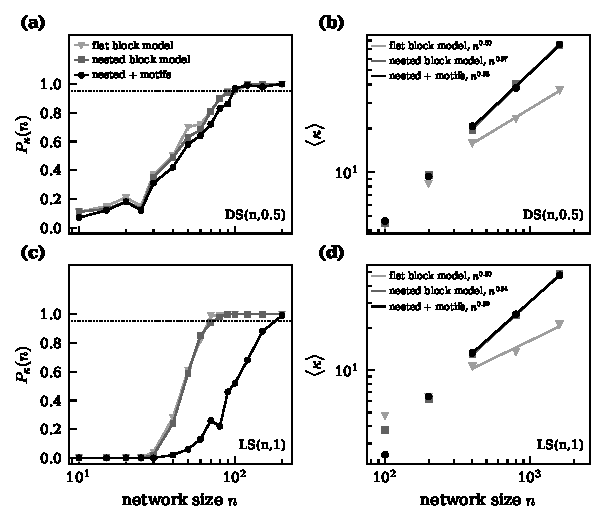
\includegraphics[width=\linewidth]{figs/fig-gr-ramsey.pdf}
  \caption{\textbf{The detection method is part of the answer.} Every panel
  compares three methods on identical networks: a flat block model, a nested one,
  and the nested one with triangles and squares in its alphabet.
  \textbf{(a)}~duplication--split, \textbf{(b)}~local search. The communities
  likelihood $P_\kappa(n)$, from a hundred networks at each size up to $n=200$
  and twenty above it, with the dotted line at the $95\%$ threshold whose
  crossing defines the Ramsey community number. Duplication--split makes no
  triangles and the three curves lie on top of one another; local search
  \emph{is} the triadic-closure rule, and naming its triangles moves the crossing
  from $80$ to $200$.}
  \label{fig:gr-ramsey}
\end{figure}

$BB(n,1)$, which closes triangles by a quite different mechanism --- laying a
single new node across a random link rather than closing a path --- behaves like
local search and not like its own square-closing sibling. Its onset moves from
$100$ to $400$ and nothing else happens: past the threshold the motif model's
community count converges on the nested model's rather than collapsing away from
it, $5.6$ against $5.8$ at $n=200$ and $11.1$ against $11.9$ at $n=400$, and its
exponent is $0.892$ with the alphabet against $0.886$ without it.

The pseudofractal web looks at first like the same story told deterministically
--- $1.02$ against $0.99$, a lattice built entirely of triangles whose density
appears untouched by being allowed to name them --- and it is not. That reading
comes apart in Section~\ref{sec:gr-square}, and it comes apart in a way that says
something about the instrument rather than about the lattice. It is left out of
this section for that reason, and so is the diamond.

So where the alphabet names the rule's own motif, it postpones the onset by a
factor of two to four and leaves the exponent alone. That is the first route into
this class, and the more informative one, because the alphabet was working and
the density survived anyway.

\subsection*{Where the alphabet names nothing}

The second route is duplication with divergence, and its entry in the table is
the $0\%$ in the last column: at $n=800$ the alphabet succeeds in naming
essentially none of the network's links. That is not for want of squares.
$DD(n,q)$ copies a random node and deletes each copied link independently with
probability $q$; it never subdivides anything, so unlike duplication--split it
stays bipartite, and counted directly at $q=\tfrac12$ it has mass at the even
lengths and exactly nothing at the odd ones:

\begin{center}
\begin{tabular}{lrrrrrr}
\hline
 & \multicolumn{6}{c}{number of cycles of length $L$}\\
$DD(n,\tfrac12)$ & $L=3$ & $4$ & $5$ & $6$ & $7$ & $8$ \\
\hline
$n=100$ & $0$ & $694$ & $0$ & $9\,099$ & $0$ & $123\,001$\\
$n=200$ & $0$ & $3\,658$ & $0$ & $143\,822$ & $0$ & $7\,002\,135$\\
\hline
\end{tabular}
\end{center}

\noindent By the reading of Section~\ref{sec:gr-conjecture} this is a square-built
network if ever there was one, and the motif model declines to plant a single
square in it. Fitted at $q$ from $0.2$ to $0.6$ the enlarged alphabet buys
nothing: it costs a few tens of bits on average, and the scatter between repeated
fits of the same network is larger than the cost, so the only thing the number
says is that nothing was gained.

The reason is that duplication does not make a square. It makes a node with $d$
shared neighbours --- a complete bipartite $K_{2,d}$ --- holding $\binom{d}{2}$
four-cycles laid over one another. At $n=200$ and $q=\tfrac12$ the sharing runs
to fourteen common neighbours between one pair of nodes, so that pair alone
accounts for $91$ four-cycles, and across the network each link sits in some
twenty-four of them. A decomposition that gives every link to exactly one motif
can name a handful and must leave the rest unspoken.

That diagnosis blames the alphabet for lacking a symbol, which is a testable
complaint, and the test is to supply the symbol. Add the biclique $K_{2,d}$: two
hubs joined to the same $d$ leaves, $d+2$ nodes and $2d$ links. Its automorphism
group has size $|\mathrm{Aut}|=2\,d!$ --- the two hubs may swap, and the $d$
leaves permute freely --- which is what Eq.~\eqref{eq:gr-omega} divides by so
that one planted copy is charged once rather than once per way of writing it
down. It is exactly what duplication builds, and $d=2$ is the square, so the
family starts at $d=3$. On a network of planted bicliques it does what it should.
Twenty disjoint $K_{2,6}$, which is $240$ links:

\begin{center}
\begin{tabular}{lrl}
\hline
alphabet & $\Sigma$ (bits) & planted\\
\hline
link only            & $1820$ & ---\\
$+$ triangle, square & $1415$ & $60$ squares\\
$+$ biclique         & $\mathbf{1028}$ & $20$ $K_{2,6}$\\
\hline
\end{tabular}
\end{center}

\noindent The square alphabet carves each biclique into three disjoint squares
and pays $387$ bits more than naming it once. (Bicliques have to be offered
before squares, or the squares consume the links first and the larger object can
never be seen --- a reminder that a greedy search over a nested vocabulary must
work from the largest symbol down.)

Now duplication--divergence, with everything in one block. The model finds $760$
biclique candidates in $DD(n{=}200,q{=}\tfrac12)$ and plants twenty-four of them,
two as large as $K_{2,14}$, taking $\Sigma$ from $3711$ to $3458$: a saving of
$252$ bits where the square alphabet saved nothing at all. The vocabulary was not
the problem. Given the symbol, the model names the structure and profits by it.

What defeats it is the partition. Refit the same network with the block model's
own division into eleven groups, and the number of biclique candidates is
\emph{zero}. Not few --- none. Every duplicated pair has been separated from its
shared neighbours by a block boundary, and a motif that straddles a boundary is
not representable at all.

That is a more damaging limitation than the missing symbol, and it is
self-inflicted. The restriction of motifs to the inside of a single block is what
kept the parameter count at $3B+B^2$ rather than the $B^4/24$ of a tensor, and so
kept the resolution at $\sqrt{n}$ instead of $n^{1/4}$
(Section~\ref{sec:gr-motifsbm}). The saving is real. It also happens to break the
scheme on the one rule that most needs it, because duplication puts a copy and
its original in different groups --- they have the same neighbours but need not
be joined to each other, which is exactly the configuration a block model splits.
Worse, the two descriptions cannot be combined. One block with the bicliques
named costs $3458$ bits; eleven groups with nothing named costs $3163$; and there
is no fit that has both, because choosing the groups destroys the motifs. The
block structure wins by some three hundred bits, so the model reports communities
and no motifs --- but it reports them by default rather than by preference,
having been given no option that keeps the duplication visible.

Adding self-interaction does not rescue it. The duplication rule of
Chapter~\ref{ch:duplication} allows the copy to bind its own original with some
probability $p$, and since the pair already shares neighbours, every such link
closes triangles. At $p=0.1$ and $q=0.45$ the network is no longer bipartite, the
odd cycle lengths fill in, and the clustering coefficient rises from zero to
about $0.18$ and stays there as the network grows --- the interactome-like
behaviour that motivated the rule. The alphabet still plants nothing: at $n=100$,
$200$ and $400$ the enlarged model costs bits rather than saving them. The
triangles stack exactly as the squares did, all of those at a duplicated pair
sharing the one link between the pair, so that a single link can carry eleven of
them and an edge-disjoint decomposition can name at most one per pair.
Duplication defeats the alphabet whether or not it makes triangles, because
everything it builds is piled onto the same shared neighbourhood.

So duplication reaches the constant-density class by the uninteresting route: its
$\beta$ is $1.11$ with the alphabet and $1.12$ without it because the alphabet
never got started. A rule whose footprint is a biclique of variable size, laid
over a shared neighbourhood the partition wants to cut, is out of reach of a
scheme that names fixed objects inside single blocks --- and that is the rule
most often proposed for how protein interaction networks grow.

A last caution, which applies to every $\Delta\Sigma$ quoted in this chapter. The
fit is a stochastic search, and repeated fits of the \emph{same} network return
description lengths that differ. For $DD(n,q)$ at $n=400$ the spread over five
fits is around $150$ bits, larger than most of the differences being compared.
Where a sign is reported here it is the sign of an average, and the small numbers
should be read as saying that nothing was gained rather than as measurements of
how much was lost.

\section{The rule with no communities left}
\label{sec:gr-none}

$BB(n,2)$ is the one rule in the table that the alphabet moves into the first
class. Both block models put its Ramsey community number at $400$; the motif
model never reaches the $95\%$ threshold at all. Its likelihood peaks near $0.65$
around $n=1600$ and then falls away --- $0.20$ at $3200$, and at $6400$ every one
of ten realisations returns a single community while the block model returns a
hundred and two (Figure~\ref{fig:gr-squares}a).

Pushed to larger sizes, that statement turns into something more awkward than a
suppression. The motif model's answer for $BB(n,2)$ is not small, it is
\emph{bimodal}. At $n=3200$, sixteen realisations in twenty return a single
community and the other four return between thirty-five and forty-one, which is
what the block model returns throughout. One description plants many squares and
needs no communities at all; the other finds the communities and plants fewer
squares; and which of them comes back is settled by where the search happens to
start.

Whether the criterion is \emph{indifferent} between them is a separate question,
and it has to be asked carefully, because the obvious way of asking it gives the
wrong answer. Comparing the mean $\Sigma$ of the realisations that landed on one
community with the mean of those that landed on many puts them eleven bits apart
in fifty-one thousand, which invites the conclusion that the two descriptions
cost the same. They do not. That comparison is between \emph{different networks},
sorted by which answer the search happened to find, so it measures which networks
are easy at least as much as which description is shorter.

The comparison to make is on one network at a time: fit it twice under the same
alphabet, once from a single block, so that motifs are promoted before any
partition exists, and once from the nested model's own partition, so that the
communities are there first and the motifs must pay to displace them. Both are
local minima --- neither search ever leaves the basin it started in --- so the
two descriptions can be priced against each other on identical data.

\begin{center}
\small\setlength{\tabcolsep}{4pt}
\begin{tabular}{lrr}
\hline
$BB(n,2)$, both fits on one network & $n=1600$ & $n=3200$\\
\hline
$\kappa$ from one block             & $1.0$ & $1.0$\\
$\kappa$ from the partition         & $22.6$ & $42.8$\\
$\phi$, links named, from one block & $0.57$ & $0.57$\\
$\phi$ from the partition           & $0.29$ & $0.27$\\
\hline
$\Delta\Sigma$ (bits)               & $-203$ & $-627$\\
$\Delta\Sigma/n$ (bits/node)        & $-0.13\pm0.05$ & $-0.20\pm0.08$\\
spread between networks (bits)      & $378$ & $903$\\
communities win                     & $40\%$ & $8\%$\\
\hline
\end{tabular}
\end{center}

\noindent Priced this way the motif description wins outright, and the margin per
node grows rather than shrinking. The criterion is not indifferent; it has
decided, and it decides more firmly as the network grows.

What is true is that the decision is smaller than the scatter. The
network-to-network spread is about half again the gap at both sizes, so an
individual realisation lands on either side, and that is what produces the
bimodality. It is also why the sorted comparison misleads: with a gap narrower
than the noise, sorting realisations by outcome and then averaging recovers
almost nothing of it.

So the squares and the communities are two ways of spending the same bits on the
same links, and for this rule they cost \emph{nearly} the same --- near enough
that the search's starting point decides any single case, not near enough that
the criterion is silent. That is why $BB(n,2)$ carries no motif-model exponent in
the master table: its mean $\kappa$ is the mixing ratio of two outcomes rather
than a law, and it turns over at $n=3200$ for that reason and no other.

There is a control for all this, and the rule that provides it differs from
$BB(n,2)$ in one place only. The bubble rule lays a chain of $L$ new nodes across
a random link and so closes a cycle of length $L+2$: squares at $L=2$, and
triangles at $L=1$. If what dissolved the communities was the square, or the mere
fact that a motif in the alphabet matches the rule, then $BB(n,1)$ should
dissolve the same way. It does not --- it sits in the previous section, its onset
merely postponed. Nor is the difference that triangles are harder to name than
squares: counting what the fits actually plant at $n=200$, $BB(n,1)$ plants $62$
triangles covering forty-seven per cent of its links and $BB(n,2)$ plants $40$
squares covering fifty-three per cent, and the master table's last column has
them at $54\%$ and $57\%$ at the largest sizes fitted. Comparable effort,
opposite outcome.

Something on the other side of the ledger must be doing it --- how much community
structure there was to destroy. $BB(n,2)$ is a marginal community-former to begin
with, its block-model Ramsey number of $400$ standing at four times $BB(n,1)$'s,
and a margin narrow enough for the starting partition to decide the outcome is
only reachable when the partition's own contribution is thin. A tenth of a bit
per node is what a thin one looks like.

That is an observation about $BB(n,2)$ rather than a rule, and it should not be
promoted into one: a thin partition is what makes the contest close, but it does
not by itself say which way the contest goes. Settling that needs the bubble
family swept across $L$ rather than sampled at two values of it --- a question
for the family, and not one this chapter can answer from two of its members. What
this section establishes is narrower and does not depend on the answer --- that an alphabet can abolish a rule's communities outright, and that
the rule it does it to is not the one a reading based on the motif's shape would
have picked.

\begin{figure}[t]
  \centering
  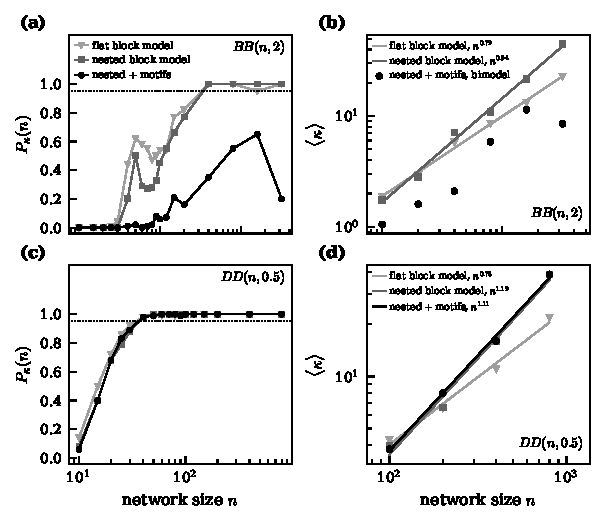
\includegraphics[width=\linewidth]{figs/fig-gr-squares.pdf}
  \caption{\textbf{Two rules built from squares, and only one of them says so.}
  Panels as in Figure~\ref{fig:gr-ramsey}: $P_\kappa$ from a hundred networks at
  each size up to $n=200$ and twenty above it. \textbf{(a)} $BB(n,2)$ closes one
  square per step on two new nodes, so its squares are nearly disjoint, the
  alphabet takes them up, and the communities the block model reports are largely
  dissolved. \textbf{(b)} $DD(n,q)$ at $q=\tfrac12$ closes squares in far
  greater numbers, but as overlapping $K_{2,d}$ bicliques rather than separable
  motifs; the alphabet plants none of them, and all three methods agree.}
  \label{fig:gr-squares}
\end{figure}

\section{The lattices that describe themselves}
\label{sec:gr-square}

Two lattices are left, and they are the ones on which the alphabet does the most
and the search does the worst. Taking them together is what empties the fractal
class and puts both of them in the first.

The pseudofractal web hangs a new node on both ends of every link, closing a
triangle; the diamond replaces every link by two parallel paths of one node each,
closing a square. Both reach exactly two steps --- every new node is adjacent to
nodes that were already adjacent --- and both rebuild the whole lattice at once,
which is what keeps their cycles clean, since a rule that subdivides one link at a
time stretches the cycles it has already made. They differ in the cycle they
close and in almost nothing else.

Fitted, they look like a clean contrast. Both sit at the modular limit under the
nested block model, $1.02$ and $1.05$, and under the motif alphabet the
pseudofractal reads $0.99$ while the diamond falls to $0.31$; the diamond's fit
returns $3$, $5$ and $7$ groups at $n=684$, $2732$ and $10\,924$, a count
climbing by a fixed amount while the lattice quadruples. That contrast was the
original reading of this section, and it does not survive.

\subsection*{Both lattices tile themselves exactly}

Each of these rules gives every existing link exactly one new motif per
generation. So the motifs closed at the \emph{last} generation have distinct old
links and disjoint new chains, and between them they use every link in the
network exactly once. A perfect edge-disjoint tiling of the lattice by its own
motif exists at every size, in both lattices, and it can be written down from the
construction without fitting anything: $729$ triangles for the $2187$ links of
the pseudofractal at $n=1095$, $1024$ squares for the $4096$ links of the diamond
at $n=2732$.

Price that decomposition and compare it with what the search finds:

\begin{center}
\footnotesize\setlength{\tabcolsep}{5pt}
\begin{tabular}{lrrrrrr}
\hline
 & & \multicolumn{2}{c}{as fitted} & \multicolumn{2}{c}{the tiling} & \\
lattice & $n$ & $\Sigma$ & $\kappa$ & $\Sigma$ & $\kappa$ & cheaper by\\
\hline
pseudofractal & $366$    & $4\,474$   & $5$  & $3\,887$   & $1$ & $587$\\
pseudofractal & $1\,095$  & $15\,428$  & $14$ & $13\,728$  & $1$ & $1\,700$\\
pseudofractal & $3\,282$  & $53\,082$  & $44$ & $47\,673$  & $1$ & $5\,409$\\
diamond       & $684$    & $7\,812$   & $3$  & $7\,434$   & $1$ & $378$\\
diamond       & $2\,732$  & $37\,213$  & $5$  & $35\,666$  & $1$ & $1\,547$\\
diamond       & $10\,924$ & $171\,368$ & $7$  & $166\,876$ & $1$ & $4\,493$\\
\hline
\end{tabular}
\end{center}

\noindent The tiling is cheaper at every size, on both lattices, by a margin that
grows with the network. Handed to the optimiser as a starting state it does not
move off it. And it uses \emph{one} community: a single block, every link spoken
for by a motif, nothing left for a partition to explain.

So on the criterion this chapter has used throughout, the best available
description of the pseudofractal web has no communities --- not the fourteen the
fit reports at $n=1095$, and not the forty-four it reports at $n=3282$ --- and the
same is true of the diamond. The two rules are in the same class. Their
description lengths are not merely similar but equal to the bit where their sizes
coincide, $7434$ at $n=684$ and $35\,666$ at $n=2732$, because both are tiled by
their own motif on the same $n$ and $m$.

\subsection*{What that costs, and what it does not}

It costs the contrast. The pseudofractal was this section's foil --- the lattice
that keeps its law while the diamond loses it --- and there is no such foil.
Along with it goes the argument that reach cannot be the discriminator because
two rules of equal reach end up in different classes: they do not end up in
different classes. Chapter~\ref{ch:communities}'s ranking of a triangle rule
against a square rule may still be telling us something, but not this.

It does not cost the finding. The diamond's own result is strengthened rather
than weakened: an alphabet can take a network's communities away entirely, and
under the best description available the diamond has none at all, rather than the
vanishing density earlier arithmetic gave it. What was reported as $\kappa$
growing like $\log n$ was a partition the search was carrying and did not need.

Nor does it touch the comparison that made the finding safe. Reducing the
alphabet to the link alone recovers the ordinary degree-corrected model exactly
(Section~\ref{sec:gr-motifsbm}), and on the diamond it costs $8908$, $41\,929$
and $198\,987$ bits at the three sizes against the motif description's $7434$,
$35\,666$ and $166\,876$ --- margins of a sixth rather than the eighth the fitted
comparison gave. The motif description wins by more than was claimed, not less.

The awkward part is what it says about the instrument. These are the two networks
in the book whose optimal description can be written down by hand, and they are
the two where the greedy search is furthest from it --- by up to a tenth of the
whole description length. That is not a coincidence, and
Chapter~\ref{ch:bubbles} takes it up: a deterministic rule builds an exact
optimum, and an exact optimum is a thing a greedy search can exactly miss. Every
other rule in this book is stochastic, lays its motifs across links chosen at
random, and has no such optimum to be missed.

\section{What decides the class}
\label{sec:gr-decides}

Three classes, and two rules that changed class when the vocabulary changed. What
is it about a rule that decides which way it goes?

Not the motif's shape: triangles dissolve nothing on local search or $BB(n,1)$
and everything on the pseudofractal, and squares dissolve everything on
$BB(n,2)$ and the diamond while doing nothing whatever on $DD(n,q)$ or
duplication--split. What the master table's last column measures is the one
quantity that separates the cases at the ends: how many of a network's links an
edge-disjoint decomposition can take up.

At one end sit the two lattices, at a hundred per cent. Each gives every link one
new motif per generation, so the last generation's motifs tile the whole network,
and a partition is left with nothing to explain --- which is exactly what the fit
finds when it is started from the tiling, one community and no residue
(Section~\ref{sec:gr-square}). At the other sits duplication--divergence at
nought per cent, where every square is stacked on the same shared neighbourhood
and a decomposition that gives each link to one motif can name almost none of
them; there the alphabet never engages and the partition keeps all of its work.

That is the mechanism where it can be seen cleanly. Where the motif tiles the
network, the partition has nothing left to describe and the communities go. Where
the motifs overlap, they cannot absorb what the partition was explaining, and the
communities survive. The same overlap that made duplication's bicliques
unnameable is here doing something useful.

Both ends are extremes, and it is worth saying what makes them legible. A
hundred per cent against nought is not a marginal gap, and the lattices are
deterministic --- one network per size, no sampling, and a decomposition that can
be checked by construction rather than searched for.

Between the ends the account has nothing to say, and the last column says so
plainly.
$BB(n,1)$ names $54\%$ of its links and keeps its communities; $BB(n,2)$ names
$57\%$ and loses them; local search names $62\%$, more than either, and is in no
danger at all. Three rules within eight points of each other on the quantity that
is supposed to be deciding, and two different outcomes. Whatever separates
$BB(n,1)$ from $BB(n,2)$, it is not how much of the network their motifs can take
up, and no reading of that column will supply it.

What does separate them is a question about the bubble family rather than about
this chapter's three classes, and the family repays being taken on its own terms:
$L$ is a dial, the rule is otherwise fixed, and the whole sequence can be fitted
with the alphabet extended to name each rule's own cycle. That is done
separately. What belongs here is the negative: the tiling account earns the two
lattices and does not earn the rest, and the difference between $BB(n,1)$ and
$BB(n,2)$ is left open by it.

What can be said from this side is what happens when nothing is taken up.
$BB(n,1)$ grows its communities as $n^{0.892}$ with the alphabet and $n^{0.886}$
without it, over $n=400$ to $3200$ --- indistinguishable. A motif the
decomposition cannot lay down over the network costs that network's density
nothing, whatever else is going on.

The caution generalises past any one rule. Wherever an alphabet can absorb the
same links that a partition would have explained, the two descriptions trade off
against each other, and the margin between them can fall below the
network-to-network scatter --- at which point the criterion still has a
preference but no single fit reliably reports it, and what comes back is decided
by where the search began. That is a limit on what any such method can be asked
to settle from one realisation, and not a defect of this implementation.
$BB(n,2)$ is that limit made visible: a real preference of a tenth of a bit per
node, carried on a scatter half again as large.

\begin{quote}
\emph{To follow up.} Chapter~\ref{ch:graphons} measured the community density of
three real growing networks with a vocabulary that could not name a triangle, and
the diamond shows that such a vocabulary can flatter a network into a density it
does not have. Whether the Internet and the yeast interactome keep $\beta=1$
under the full alphabet is being measured and is not settled here; the
collaboration graph, at sixty thousand nodes, is beyond what the motif fit can
reach at present. The interesting outcome would be the third class. A real
network landing at $\tfrac12<\beta<1$ and staying there under motif correction
would be the first genuinely fractal community structure in this book ---
Chapter~\ref{ch:communities}'s $0.61$ having turned out to be the flat model's
ceiling, and Chapter~\ref{ch:graphons}'s $0.80$ a sample that mixed grown
networks with catalogued ones.
\end{quote}

\section{Which change moves which number}
\label{sec:gr-doubledissoc}

Three methods have been compared through these sections, and they differ in two
ways rather than one. Flat against nested is a difference of resolving power and
nothing else; nested against nested-with-motifs is a difference of vocabulary and
nothing else (Section~\ref{sec:gr-motifsbm}). Reading the master table of
Section~\ref{sec:gr-classes} across rather than down, the two differences turn
out to move two different quantities, and it is worth separating them because
one of them is a great deal better behaved than the other.

Where the first difference comes from was the subject of
Chapter~\ref{ch:graphons}, and was priced there exactly: the two models express
the same partitions and differ only in what naming one costs, the flat model
paying a charge quadratic in the number of groups and so meeting
Eq.~\eqref{eq:gr-flatceiling}'s ceiling of $\sqrt n$, the nested model
compressing the group-level structure instead and reaching
Eq.~\eqref{eq:gr-nestedceiling}'s $n/\log n$. Nothing in that arithmetic mentions
what the links are made of.

\emph{Resolution moves the exponent, and only the exponent.} Going from the flat
model to the nested one lifts $\beta$ by two to four tenths on every rule in the
table without exception, and moves the onset $r_\kappa$ by at most a seventh ---
$70$ to $80$, $90$ to $100$, $400$ to $400$, $40$ to $40$. It never changes a
rule's class, because it cannot: the flat model's fractal-looking exponents are
its ceiling, and lifting the ceiling reveals the density that was there all
along.

\emph{Vocabulary moves the onset, and sometimes the class.} Naming a rule's own
motif moves $r_\kappa$ by a factor of two to four --- $80$ to $200$ for local
search, $100$ to $400$ for $BB(n,1)$, and at least four and perhaps sixteen for
the diamond, whose generations are too far apart to pin down --- and leaves it
untouched where the alphabet has nothing to name, as with duplication--split and
duplication--divergence. On the five random rules where the alphabet cannot take
up the whole network it leaves $\beta$ alone to within a hundredth or two. On the
three where it can, it does something the resolution
knob cannot do at all: it moves the rule out of the constant-density class
entirely --- $BB(n,2)$, the diamond and the pseudofractal all into the first,
with no communities left at all.

So the tidy statement --- one knob for how finely a network can be cut, another
for whether there is anything to cut --- holds for most of the table and fails in
exactly the cases this chapter was written about. The failure is not a
complication to be regretted; it is the finding. A vocabulary that
\emph{cannot} take up the whole network leaves the exponent alone, and that is
the common case. A vocabulary that can take up the whole network takes over the
description, and then the exponent is not measuring the network's communities any
more but the leftovers of a tiling.

The asymmetry has a reason. The exponent is a statement about how finely a
network can be cut, and nothing about the vocabulary for describing links changes
how many groups a method is \emph{able} to resolve --- that ceiling is fixed by
what the description length charges for the block structure. But the vocabulary
does change how many groups are \emph{worth} resolving, by offering an
alternative account of the same links; and where that alternative can cover
everything, the number of groups worth resolving falls to almost none. The
ceiling and the demand are different things, and only the second is open to the
alphabet.

This also tidies up a conclusion that has been uncomfortable since
Chapter~\ref{ch:graphons} drew it: that Chapter~\ref{ch:communities}'s exponent
is in part a statement about the flat block model rather than about the networks.
It can now be said without reference to motifs at all. On the rules where the alphabet cannot tile, it is
irrelevant to $\beta$; the whole of the shift from $0.61$ is the nested model,
which is a standard tool and not one invented here. Whatever else is uncertain
about the machinery of these sections, that conclusion does not rest on it.

And it answers, with one qualification, the question Chapter~\ref{ch:graphons}
left at its door. What that chapter found was a density: with the resolution
lifted, the number of communities grows in proportion to the size, so $b=B/n$
becomes a number a network has rather than a rate at which something grows. The
obvious worry about such a quantity is that it might be an artefact of a poor
vocabulary --- that a model forced to describe every triangle as three separate
links would invent communities to absorb what it could not name, and that a
richer alphabet would dissolve them. On the rules whose motifs overlap it does
not: give the model triangles, squares and bicliques and the density stays where
the nested prior put it. The qualification is the three rules whose motifs do not
overlap --- $BB(n,2)$ and the two lattices --- where exactly that worry is
realised, and it is why Chapter~\ref{ch:graphons}'s conjecture has to be read as
a claim about the best available description rather than about the network
itself.

Two instrument effects had already been found and separated before this chapter
began, and it is worth noticing that all three were found the same way.
Chapter~\ref{ch:communities}'s $0.61$ became $0.80$ when the prior stopped
charging quadratically for groups, and $0.80$ became $1$ when the sample stopped
mixing grown networks with catalogued ones. Neither move was about networks. What
this chapter adds is a third of the same kind and a sharper one: change the
vocabulary and a network can change not merely its exponent but the class it
belongs to. A limit class, like an exponent, is a property of a network together
with the code used to describe it.


\chapter{Eureka: Motifs are blueprinted communities}
\label{ch:bubbles}

Chapter~\ref{ch:motifs} ended in a state that ought to be uncomfortable. The same
networks, counted by three methods differing only in what they are permitted to
say, gave community counts a hundred apart --- $BB(n,2)$ at $n=6400$ reads
$102$ communities under a nested block model and one under the same model with
squares in its alphabet. Three rules changed limit
class when nothing about them changed but the vocabulary. And the quantity
Chapter~\ref{ch:graphons} had offered as what a locally grown network converges
to --- the density of communities, constant in size and set by the rule --- came
out as one number under a block model and another under a block model that can
name a square. A quantity that moves that far when the describer's vocabulary
changes invites the question whether it was measuring the network at all.

This chapter is the answer, and the answer is not that the disagreement was a
mistake. It is that the two vocabularies were counting the same thing in
different units.

The hypothesis takes one sentence, and the rest of the chapter is what happens
when it is taken seriously. A motif and a community are the same object at two
scales. Both are the description saying \emph{these nodes belong together, and
here is how they are joined}. A motif says it from a blueprint --- a template
fixed in advance, identical in every copy, paid for once and then stamped out
wherever it fits. A community says it bespoke --- a size and an internal density
inferred for that group alone, paid for again for every group. Neither is more
real than the other. They are two ways of buying the same structure, and minimum
description length shops for the cheaper.

Follow that and a good deal of what looked like instability turns into
bookkeeping. A rule whose footprint can be stamped over the whole network needs
no bespoke groups and reports none. A rule whose footprint overlaps itself can be
only partly stamped, and whatever the blueprint cannot cover has to be bought at
the bespoke rate --- which is what a community is. The community count stops
being a property of the network and becomes the size of a remainder. What does
not move is the total.

That is a claim about descriptions rather than about any one network, so testing
it needs a family and not an example: rules that differ in their local structure
and in nothing else, so that the remainder can be made to grow and shrink while
everything around it is held still.

The bubble model is that family, and it is the reason this chapter exists.
$BB(n,L)$ of Chapter~\ref{ch:communities} lays a chain of $L$ new nodes across a
randomly chosen existing link, closing a fresh cycle of length $L+2$; it is the
only rule in this book with a knob that changes the local structure and nothing
else. The reach changes with $L$, and so does the density, but the construction,
the attachment rule and the growth are fixed. Sweeping $L$ from one to five, and
then building two variants of $L=2$ that break the pattern deliberately, puts
rules on both sides of Chapter~\ref{ch:motifs}'s divide and lets us ask what
survives the crossing. The answer, when it comes, is a single number that does
not care which side a rule is on --- but the route to it runs through an
alternation nobody predicted, a lattice that describes itself, and one experiment
whose result was called in advance and came out right.

\section{A dial for the shortest cycle}
\label{sec:bb-dial}

\begin{figure}[t]
  \centering
  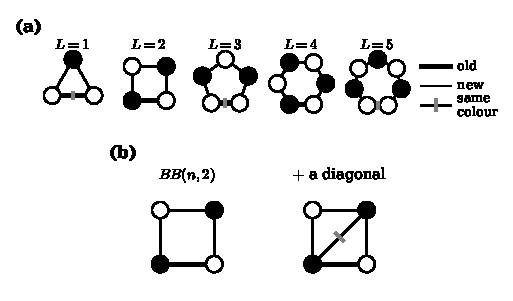
\includegraphics[width=\linewidth]{figs/fig-bb-parity.pdf}
  \caption{\textbf{Two-colouring the $L+2$ cycle.} It closes for even $L$. For
  odd $L$, or for any $L$ once a diagonal is added, one link is left with both
  ends the same colour.}
  \label{fig:bb-parity}
\end{figure}

What $L$ controls is the shortest cycle the rule ever closes, and through it the
whole cycle spectrum. Two faces sharing a link close a cycle of length $a+b-2$,
so the lengths present are generated by the motif and its gluings and everything
else is empty: $BB(n,1)$ carries every length, $BB(n,2)$ carries $4,6,8,10$,
$BB(n,3)$ carries $5$ and $8$, $BB(n,4)$ carries $6$ and $10$. The clustering
coefficient follows the same arithmetic --- $0.74$ at $L=1$ and exactly zero for
every $L$ above it, since no rule but the first closes a triangle.

Chapter~\ref{ch:communities} already measured what the dial does to the onset of
communities, and the answer was not a clean monotone. The Ramsey community number
climbs steeply with $L$, from $108$ at $L=1$ to fifty-six thousand at $L=9$, and
riding on the climb is an alternation: $246$ at $L=3$ against $326$ at $L=2$ and
$2201$ at $L=4$; $752$ at $L=5$ against $2201$ below it and $6595$ above.
\emph{Every} odd $L$ sits beneath both of its even neighbours. Communities come
on sooner when the cycle the rule closes is odd, and that chapter recorded the
effect without explaining it.

The measurements here reproduce it where the grid allows. Fitting the flat
degree-corrected block model on sizes $100,200,400,\ldots$, the onsets come out
at $90$, $400$, $400$, $1600$ and $800$ for $L=1$ to $5$, against the published
$108$, $326$, $246$, $2201$ and $752$. The two middle values collapse onto one
grid point --- $326$ and $246$ are not separable at a spacing of two --- but
$L=4$ against $L=5$ is resolved and comes out the right way round, $1600$ against
$800$, and the $L=5$ figure agrees with the published $752$ to within the grid.
That the odd rules form communities sooner is not an artefact of one
implementation.

\section{Extending the alphabet}
\label{sec:bb-alphabet}

Chapter~\ref{ch:motifs} fitted these networks with an alphabet of the link, the
triangle and the square. Run $BB(n,3)$ through it and the fit plants nothing:
there are no triangles in a pentagon-built network and no squares either, so the
enlarged model costs the price of announcing two totals that turn out to be zero
and buys nothing. Read the output naively and $BB(n,3)$ is a rule whose community
density is untouched by the motif alphabet --- filed alongside
duplication--divergence, in the class where the vocabulary makes no difference.

That reading would be worthless, and the reason is the lesson
Chapter~\ref{ch:motifs} spent itself establishing, turned on the instrument that
established it. A class is a property of a network together with the code used to
describe it. An alphabet with no symbol for a pentagon cannot be asked whether
naming pentagons dissolves communities; it can only report that it has no
pentagons to name. The whole point of the exercise is to give each rule a
vocabulary equal to its own footprint and then see what happens, and for $L>2$
that vocabulary did not exist.

So the alphabet is extended by the cycles above the square. An $L$-cycle has
$|\mathrm{Aut}|=2L$, the dihedral group of $L$ rotations and a reflection, which
is the number Eq.~\eqref{eq:gr-omega} divides by so that one planted copy is
charged once rather than once for every way of writing it down; the convention
checks out, since $k!/|\mathrm{Aut}|=(k-1)!/2$ returns twelve distinct
five-cycles on five labelled nodes, sixty six-cycles on six, and three hundred
and sixty seven-cycles on seven. The triangle and the square keep the
special-cased enumerators they always had, so nothing measured before this family
existed can have moved.

Every rule below is then fitted twice on the same networks: once with the
\emph{control} alphabet of link, triangle and square, which is
Chapter~\ref{ch:motifs}'s and which for $L>2$ has no symbol for the rule's own
cycle, and once with the \emph{test} alphabet, the same plus the $L+2$ cycle.

The control is not decoration. It is the check that the extended fit
reduces to the nested block model when it has nothing to name, and it does: on
$BB(n,3)$ at $n=3200$ the control returns $24.3$ communities against the nested
model's $24.1$. Whatever the test column then reports is the alphabet at work and
not a change of software.

\section{The family}
\label{sec:bb-family}

Seven rules, twenty realisations at each size, exponents fitted from $n=400$
upward so that every rule is past its own onset and none of them contributes a
stretch of $\kappa=1$ to a slope.

\begin{center}
\footnotesize\setlength{\tabcolsep}{3pt}
\begin{tabular}{lccrrrrr}
\hline
rule & cycle & bip. & $\langle k\rangle$ & $r_\kappa$ & $\beta$ nested & $\beta+$mot. & named\\
\hline
$BB(n,1)$ & $3$ & no & $4.00$ & $100$ & $0.89$ & $0.89$ & $54\%$\\
$BB(n,2)$ & $4$ & yes & $3.00$ & $400$ & $0.98$ & --- & $57\%$\\
\quad $+$ a link, bipartite & $4$ & yes & $3.97$ & $100$ & $0.92$ & $0.94$ & $5\%$\\
\quad $+$ a diagonal & $4$ & no & $3.97$ & $100$ & $0.97$ & $0.93$ & $64\%$\\
\hline
$BB(n,3)$ & $5$ & no & $2.67$ & $400$ & $0.95$ & $0.96$ & $55\%$\\
$BB(n,4)$ & $6$ & yes & $2.50$ & $1600$ & $1.07$ & --- & $56\%$\\
$BB(n,5)$ & $7$ & no & $2.40$ & $800$ & $1.05$ & $1.08$ & $54\%$\\
\hline
\end{tabular}
\end{center}


\noindent The exponents in the $\beta$ nested column all sit near one, which is
Chapter~\ref{ch:graphons}'s modular limit: under a nested block model every
member of this family has a constant density of communities. What the alphabet
does to that density is the last two columns, and it alternates.

$L=1$, $3$ and $5$ keep everything. Their exponents are unmoved to within two
hundredths --- $0.89$ against $0.89$, $0.95$ against $0.96$, $1.05$ against
$1.08$ --- while the alphabet works hard the whole way: $BB(n,3)$ plants pentagons
covering fifty-five per cent of its links and saves $2362$ bits at $n=3200$, and
$BB(n,5)$ plants heptagons covering fifty-four per cent and saves a thousand at
$n=1600$. These are not fits in which the enlarged model declined the offer. The
motifs are named, in quantity, at a large and growing saving, and the communities
do not notice.

$L=2$ and $L=4$ lose them. $BB(n,2)$ goes from $44.7$ communities under the
nested model at $n=3200$ to one; $BB(n,4)$ goes from $11.9$ to $2.65$, its
likelihood of finding any communities at all peaking at $0.55$ near $n=800$ and
falling to $0.25$ and $0.15$ at $1600$ and $3200$. Neither carries an exponent in
the table, and for the reason Section~\ref{sec:gr-none} gave for the first of
them: the answer is bimodal, most realisations returning a single community and a
minority returning what the block model returns, so the mean is a mixing ratio
rather than a law.

The pattern is not subtle, and Figure~\ref{fig:bb-alternation}a is the whole of
it. Naming a rule's own motif abolishes its communities when $L$ is even and
leaves them exactly where they were when $L$ is odd.

The figure plots a ratio rather than the two community counts, and the reason is
worth a sentence, because it is the chapter's argument in miniature. These rules
differ several-fold in how many communities they have to begin with --- $BB(n,2)$
has three times $BB(n,4)$'s at the same size --- and that difference is exactly
what does \emph{not} decide the outcome. Dividing it out leaves one quantity per
rule, on a scale where surviving means one, and the five curves separate into two
families that nothing else about them separates.

\begin{figure}[t]
  \centering
  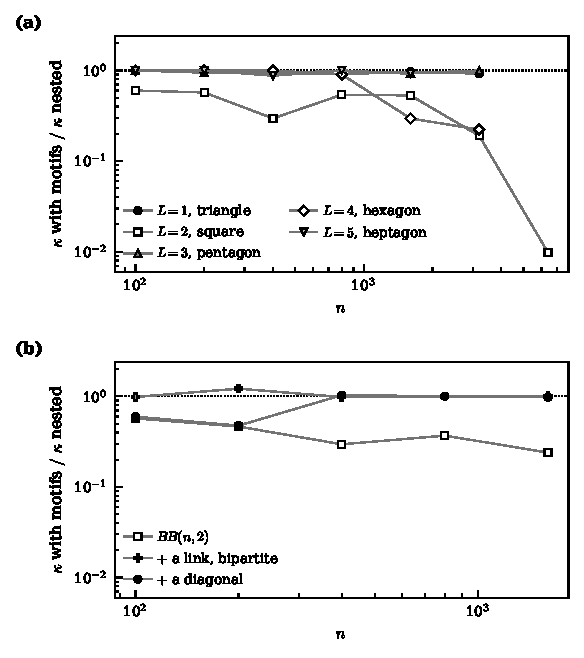
\includegraphics[width=\linewidth]{figs/fig-bb-alternation.pdf}
  \caption{\textbf{The alternation, and the diagonal that breaks it.} Both panels
  plot the community count under the motif alphabet divided by the count the
  nested block model returns on the same networks: one where the communities
  survive, falling away where they are carried off. \textbf{(a)}~$L=1$ to $5$,
  odd $L$ filled and even $L$ open. \textbf{(b)}~$BB(n,2)$ against two variants
  that each add one link per step, of which only the diagonal destroys
  bipartiteness.}
  \label{fig:bb-alternation}
\end{figure}

\section{What does not decide}
\label{sec:bb-negative}

Two explanations were available before this sweep, and the table kills both.

\subsection*{Not how much of the network the motif covers}

Chapter~\ref{ch:motifs} found that on the two deterministic lattices the
discriminator is tiling: the diamond's squares cover ninety-two per cent of its
links and its density dies, the pseudofractal's triangles reach fifty-six and its
density survives. Extended to this family the account predicts that the rules
whose motifs cover more should be the ones that dissolve.

They are not distinguishable at all. The last column reads $54$, $57$, $55$, $56$
and $54$ per cent for $L=1$ to $5$ --- a spread of three points across a family
whose outcomes are opposite. The largest coverage in the whole family belongs to
$BB(n,2)$ at fifty-seven per cent and the smallest to $BB(n,1)$ and $BB(n,5)$ at
fifty-four, and one of those three dissolves while the other two do not. Whatever
tiling explains about the lattices, where the gap is ninety-two against
fifty-six, it explains nothing here.

\subsection*{Not how much there was to lose}

The other candidate was the other side of the ledger. A near-tie in description
length is easiest to reach when the partition was not contributing much in the
first place, and $BB(n,2)$ is a marginal community-former --- a Ramsey number of
$400$ against $BB(n,1)$'s $100$. A rule with thin community structure should be
the one whose communities the alphabet can carry off.

$BB(n,4)$ and $BB(n,5)$ settle that, and they settle it against. At $n=1600$ they
have almost exactly the same amount to lose, $6.10$ communities against $6.85$
under the nested model, and their alphabets name the same share of links, fifty-six
per cent against fifty-four. One collapses to a single community and the other
does not move. If thinness were deciding, the thinner of the two would go first;
$BB(n,5)$ is the thinner by every measure in the table --- fewer communities,
lower mean degree, a later onset than $L=3$ --- and it is the one that survives.

\section{Parity}
\label{sec:bb-parity}

What is left is the one property that has been sitting in plain view since
Section~\ref{sec:bb-dial}. $BB(n,L)$ closes cycles of length $L+2$ and glues
them at shared links, so for even $L$ every cycle in the network is even and the
network is bipartite; for odd $L$ it is not. Two-colouring a grown instance of
each confirms it directly rather than by inference from the cycle spectrum: $L=2$
and $L=4$ two-colour, $L=1$, $3$ and $5$ do not.

The two rules that dissolve are the two that are bipartite. That is the whole of
the regularity, and it holds across five rules whose coverage is constant, whose
community counts vary by a factor of three, and whose mean degrees run from $2.4$
to $4.0$. This is the geometry drawn in Figure~\ref{fig:bb-parity}.


It also connects to something Chapter~\ref{ch:communities} recorded and could not
explain. The alternation in the Ramsey number is the same alternation: every odd
$L$, which is to say every non-bipartite member of the family, forms communities
sooner than either of its even neighbours. So bipartiteness is doing two things
at once in this family --- making communities harder to form in the first place,
and making them easier to argue away once a vocabulary exists that can name the
rule's motif --- and the second was invisible until an alphabet was built that
could reach past the square.

\section{The diagonal}
\label{sec:bb-diagonal}

A regularity across five rules is not a mechanism, and parity in this family is
confounded with everything else $L$ controls. The way to test it is to break
bipartiteness while changing nothing else, and the bubble rule makes that easy,
because a square has diagonals.

Take $BB(n,2)$ and, having laid the chain $u$--$a$--$b$--$v$ across the link
$(u,v)$, add one diagonal. The chain is still two nodes, the reach is unchanged,
one fresh footprint is still laid down per step, and the rule is local in exactly
the sense it was before. But $a$ and $v$ sit on the same side of the bipartition
--- that is what a diagonal of a four-cycle is --- so the added link closes two
triangles and the network stops being bipartite. Parity predicts the communities
survive. Tiling predicts they dissolve, since the footprint still tiles.

The footprint is now $K_4$ minus an edge: four nodes, five links, two triangles
sharing the diagonal, with $|\mathrm{Aut}|=4$ because the two degree-two nodes may
swap and so may the two degree-three nodes, giving $k!/|\mathrm{Aut}|=6$, one for
each choice of the missing link. It has to go into the alphabet, for the reason
of Section~\ref{sec:bb-alphabet} in a subtler form: without it the fit does not
report nothing, it reports the \emph{pieces}. On twenty disjoint copies the
link-only description costs $1820$ bits, the triangle-and-square alphabet $1415$
--- naming each object as a square with one link left over --- and the alphabet
with the symbol $1028$, planting exactly twenty. A rule fitted without the symbol
would have been measured on a description of its footprint's fragments.

Three rules were grown, because the diagonal also adds a link and densification is
the alternative account of anything that moves:

\begin{center}
\footnotesize
\begin{tabular}{llcc}
\hline
rule & extra link per step & $\langle k\rangle$ & bipartite\\
\hline
$BB(n,2)$              & ---                                        & $3.00$ & yes\\
$+$ a link             & to a neighbour of $v$, the opposite colour & $3.97$ & yes\\
$+$ a diagonal         & to $v$, the same colour                    & $3.97$ & no\\
\hline
\end{tabular}
\end{center}

\noindent The result is in the master table, and it is unambiguous. The chorded
rule keeps its communities: from $n=400$ its count is indistinguishable from the
nested model's --- $11.95$ against $11.60$, $23.15$ against $23.05$, $43.25$
against $44.30$ --- with an exponent of $0.93$ against $0.97$. And it keeps them
while the alphabet takes up \emph{more} of it than any other network in this
book: two hundred and ninety-six chorded squares at $n=1600$, sixty-four per cent
of the links named, a saving of $1272$ bits.

That is the tiling account refuted on its own terms. A footprint that covers
sixty-four per cent of the network leaves the communities untouched, while one
covering fifty-seven per cent abolishes them, and the difference between the two
rules is one link per step and the parity it destroys.

Two cautions, because the experiment is not as clean as its result.

The bipartite control did not work. It was built to hold density fixed while
keeping the network two-colourable, and it does that, but the extra link turns
the rule's disjoint squares into overlapping ones and the alphabet is left with
almost nothing it can name --- five per cent of the links, against fifty-seven
without the extra link. Its communities survive, but they survive the way
duplication--divergence's do, because no motif was ever planted, and that says
nothing about parity. A rule that is bipartite, as dense as the chorded one, and
still has separable squares would close the argument; every link that can be
added to a bipartite rule creates overlapping even cycles, and no such rule has
been found.

So density is not controlled within the three rules of this experiment: the only
one that is both bipartite and has an alphabet that engages is $BB(n,2)$ itself,
at $\langle k\rangle=3$. What closes it is the family from outside. Mean degree
runs $4.00$, $3.00$, $2.67$, $2.50$, $2.40$ down the sweep, and the outcome
alternates against that ordering rather than following it: $L=1$ survives at the
highest density in the family and $L=5$ survives at the lowest, with the two
casualties in between. Nothing monotone in $\langle k\rangle$ can produce that.

\section{The same rule, made deterministic}
\label{sec:bb-deterministic}

Everything so far has been measured on a rule that chooses one link at random per
step. Make it deterministic --- lay a chain across \emph{every} link of the
current network, at every generation --- and the family becomes a sequence of
lattices, one network per size, in the way the pseudofractal web and the diamond
lattice are lattices. Call it $DBB(n,L)$.

Two of its members are already in this book under other names. $DBB(n,1)$ hangs
one node on both ends of every link and is exactly the pseudofractal web; it
reproduces $n$ and $m$ at every generation. $DBB(n,2)$ is a cousin of the diamond
lattice rather than the lattice itself --- both quadruple their links each
generation and agree on $n$ and $m$ at every size, but the diamond \emph{replaces}
each link by two parallel paths and leaves its endpoints unjoined, while $DBB$
keeps the link and runs the chain alongside it. The counts follow from the rule:
$m_t=(L+2)^t$, $n_t = 2 + L\big((L+2)^t-1\big)/(L+1)$, and
$\langle k\rangle\to 2(L+1)/L$, the same limiting density as the random family.

Removing the randomness was meant to remove a nuisance. There is one network per
size, nothing to average over, and the alternation --- if it is there --- has to
show up in a single object rather than in a mean. What it removed instead was the
cover the randomness had been providing, and the result is a caution that applies
to Chapter~\ref{ch:motifs} as much as to this one.

\subsection*{Every one of these lattices tiles perfectly}

A generation gives every existing link exactly one chain. So the motifs closed at
the \emph{last} generation have distinct old links and disjoint new chains, and
they use $(L+2)\,m_{t-1}=m_t$ links between them: a perfect edge-disjoint tiling
of the whole network by its own motif, at every size, for every $L$. Counted
directly, $729$ of $729$ triangles on the pseudofractal at $t=7$, $1024$ of
$1024$ squares on $DBB(n,2)$ at $t=6$, $625$ of $625$ pentagons on $DBB(n,3)$ at
$t=5$. The same holds for the diamond lattice.

That is a statement about the networks, proved by construction rather than
fitted. Set against it, what the fit reports is a statement about the search:

\begin{center}
\footnotesize\setlength{\tabcolsep}{4pt}
\begin{tabular}{lrrrr@{\hskip 10pt}rrr}
\hline
 & & \multicolumn{3}{c}{as fitted} & \multicolumn{3}{c}{seeded from the tiling}\\
lattice & $n$ & $\Sigma$ & $\kappa$ & named & $\Sigma$ & $\kappa$ & named\\
\hline
pseudofractal & $366$   & $4\,724$  & $3$  & $45\%$ & $\mathbf{3\,887}$  & $1$ & $100\%$\\
pseudofractal & $1\,095$ & $15\,487$ & $16$ & $56\%$ & $\mathbf{13\,728}$ & $1$ & $100\%$\\
$DBB(n,2)$    & $684$   & $8\,459$  & $1$  & $66\%$ & $\mathbf{7\,434}$  & $1$ & $100\%$\\
$DBB(n,2)$    & $2\,732$ & $42\,837$ & $26$ & $13\%$ & $\mathbf{35\,666}$ & $1$ & $100\%$\\
diamond       & $684$   & $7\,812$  & $3$  & $88\%$ & $\mathbf{7\,434}$  & $1$ & $100\%$\\
diamond       & $2\,732$ & $37\,213$ & $5$  & $88\%$ & $\mathbf{35\,666}$ & $1$ & $100\%$\\
\hline
\end{tabular}
\end{center}

\noindent The right-hand columns are the known tiling handed to the optimiser as
a starting state and allowed to move. It does not move: it stays on the tiling,
and the description is cheaper than the fitted one every time, by $378$ bits at
the smallest and $7172$ at the largest. So on the criterion this book uses
throughout, the best available description of the pseudofractal web has
\emph{one} community, not the sixteen the fit reports at $n=1095$ --- and the same
is true of the diamond.

Two of those rows have the same description length to the bit, $7434$ at $n=684$
and $35\,666$ at $n=2732$, because $DBB(n,2)$ and the diamond are both tiled by
squares on the same $n$ and $m$. Two lattices that Chapter~\ref{ch:motifs} placed
in different limit classes are, under their best descriptions, indistinguishable.

\subsection*{The same thing happens all the way up the family}

Section~\ref{sec:gr-square} makes this argument for the two lattices
Chapter~\ref{ch:motifs} fits, and finds that both of them have one community
under their best description rather than the fourteen and the seven the search
reports. What the sweep adds is that it is not a peculiarity of those two. It is
what every deterministic member of this family does, at every $L$, for a reason
that is written into the rule: give every link a motif at every generation and
the last generation's motifs are a tiling, whatever the motif is.

So the parity that organises the random family has nothing to organise here.
$DBB(n,L)$ is in the first class for every $L$ measured, odd and even alike, and
the alternation of Sections~\ref{sec:bb-family} to \ref{sec:bb-diagonal} is a
fact about rules that choose one link at a time.

\subsection*{Why the random family is not touched}

The randomness is what makes $BB(n,L)$ measurable. Its motifs are laid across
links chosen at random, so they overlap: a link that has already been built into
one motif can be chosen again, and no perfect tiling exists to be missed. The
fifty-four to fifty-seven per cent the alphabet names there is close to what is
available, not a sixth of it, and it is stable across sizes and realisations
rather than collapsing as the network grows. That is why the alternation of
Sections~\ref{sec:bb-family} to \ref{sec:bb-diagonal} is a measurement and this
section is a caution.

It is worth saying plainly which way that cuts. A deterministic rule looks like
the cleaner instrument --- no sampling, no averaging, one object per size --- and
it is the one on which the instrument fails. Stochasticity is not noise obscuring
the structure here. It is what keeps the structure within reach of a greedy
search, by ensuring there is no exact optimum to be exactly missed.

\section{Motifs are blueprinted communities}
\label{sec:bb-meso}

There is a way of reading this whole chapter that makes the alternation less
strange, and it is worth stating because it also says what the two vocabularies
have been arguing about.

A planted motif and a community are the same kind of object at two scales. Both
are the description saying \emph{these nodes belong together, and here is how
they are joined}. A motif is small, fixed and homogeneous: a handful of nodes, a
wiring given once by the symbol, every copy identical. A community is large,
variable and heterogeneous: as many nodes as the fit wants, an internal density
given by a row of the count matrix, no two alike. Community detection, put this
way, is the representation of a network by heterogeneous motifs of unbounded size
and arbitrary internal connectivity, and an alphabet of motifs is the same
representation with the size fixed and the wiring named in advance.

That is why the two compete. They are not a structure and a description of it;
they are two dialects for the same statement about the same links, and minimum
description length is choosing between dialects. Which is also why "the alphabet
abolished the communities" was always a slightly misleading way to put it. The
meso-structure did not go anywhere. It was renamed.

The counts say so, and they read more easily if the notation admits the point.
Write $\kappa_0$ for the number of motifs the fit plants, against $\kappa$ for the
number of communities it reports: a motif is the null case of a community, the
simplest form the thing can take, fixed in size and homogeneous in wiring, and
the index says so. Follow both along the family (Figure~\ref{fig:bb-meso}):

\begin{center}
\footnotesize
\begin{tabular}{lrrr}
\hline
rule & $\beta$ for $\kappa_0$ & $\beta$ for $\kappa$ & $\beta$ for $\kappa_0+\kappa$\\
\hline
$BB(n,1)$ & $1.06$ & $0.89$ & $1.04$\\
$BB(n,2)$ & $1.02$ & $\mathbf{0.25}$ & $1.01$\\
$BB(n,3)$ & $0.99$ & $0.93$ & $0.99$\\
$BB(n,4)$ & $1.01$ & $\mathbf{0.28}$ & $0.99$\\
$BB(n,5)$ & $1.00$ & $0.70$ & $0.98$\\
\hline
\end{tabular}
\end{center}

\noindent The middle column is the alternation this chapter has been about,
running from $n^{0.25}$ to $n^{0.93}$ with the parity of $L$. The outer two do
not alternate at all. Every rule in the family plants motifs in proportion to its
size, and every rule carries meso-structure in proportion to its size, with a
slope of one to within a few hundredths in all ten cases.

The two panels of Figure~\ref{fig:bb-meso} are nearly the same picture, and that
is the point rather than a defect of it: $\kappa$ is a few per cent of $\kappa_0+\kappa$
throughout, so the total is dominated by the motifs and the communities are a
small residue. What the parity of $L$ decides is the size of that residue --- how
much of the meso-structure is left over for the heterogeneous vocabulary once the
homogeneous one has taken what it can.

\begin{figure}[t]
  \centering
  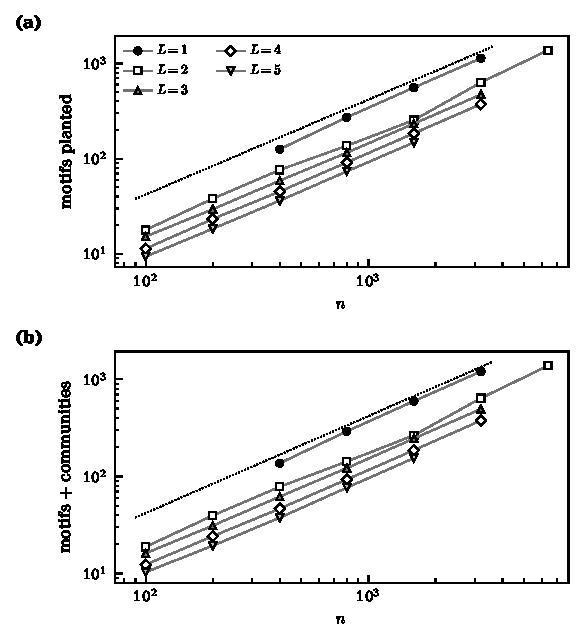
\includegraphics[width=\linewidth]{figs/fig-bb-meso.pdf}
  \caption{\textbf{Meso-structure, counted without regard to which vocabulary
  names it.} \textbf{(a)}~motifs planted, $\kappa_0$, and \textbf{(b)}~motifs plus
  communities, $\kappa_0+\kappa$, against size, with a line of slope one for the
  eye. Every rule is parallel to it in both panels, while $\kappa$ alone runs
  from $n^{0.25}$ to $n^{0.93}$ across the same five rules.}
  \label{fig:bb-meso}
\end{figure}

The density of that meso-structure is a constant of the rule, in exactly the
sense Chapter~\ref{ch:graphons} gave the density of communities: $0.38$ per node
for $L=1$, then $0.20$, $0.15$, $0.12$ and $0.09$ as the motif grows and fewer of
them fit. It falls with $L$ for a reason with no depth in it --- a longer cycle
uses more links per copy, and the mean degree is falling too --- but it is
constant in $n$ for each rule, which is the part that matters.

So Chapter~\ref{ch:graphons}'s conjecture can be restated in a form the diamond
does not break. What a locally grown network converges to is a constant density
of meso-structure. Whether a given description spends that density on motifs or
on communities is a question about the vocabulary, and the answer alternates with
the parity of the cycle; the density itself does not notice. Read that way,
$BB(n,2)$ and the diamond never lost anything. They were re-described, in a
dialect that happens to have a symbol for what they are made of.

\section{What four chapters add up to}
\label{sec:bb-conclusion}

This is the end of four chapters rather than of one, and the accounting is worth
doing in one place. Chapter~\ref{ch:communities} asked whether locally grown
networks have communities and found that they do, with a threshold size and an
exactly solvable case to show why. Chapter~\ref{ch:graphons} asked how many, and
found that the answer moved by four tenths in the exponent when the prior
changed. Chapter~\ref{ch:motifs} asked what the describer is allowed to
\emph{name}, and found that the answer could move by everything: a vocabulary
that can call a set of links a triangle sometimes reports no communities at all
where a vocabulary that cannot reports a constant density of them. This chapter
turned the one dial that changes a rule's local structure and nothing else.

Four chapters of numbers that disagree with each other invites the reading that
none of them means anything. The opposite is the case, and the last section says
why: they disagree because they are counting the same substance in two
currencies. Count it in one.

\begin{center}
\footnotesize\setlength{\tabcolsep}{5pt}
\begin{tabular}{llrr}
\hline
rule & motif & links named & $\beta$ for $\kappa_0+\kappa$\\
\hline
\multicolumn{4}{l}{\emph{no communities}}\\
\quad $BB(n,2)$ & \ngon{4} & $57\%$ & $\mathbf{1.01}$\\
\quad $BB(n,4)$ & \ngon{6} & $56\%$ & $\mathbf{0.99}$\\
\quad pseudofractal & \ngon{3} & $100\%$ & $\mathbf{1.00}$\\
\quad diamond & \ngon{4} & $100\%$ & $\mathbf{1.00}$\\
\hline
\multicolumn{4}{l}{\emph{constant density of communities}}\\
\quad $LS(n,1)$ & \ngon{3} & $62\%$ & $\mathbf{1.01}$\\
\quad $BB(n,1)$ & \ngon{3} & $54\%$ & $\mathbf{1.04}$\\
\quad $BB(n,3)$ & \ngon{5} & $55\%$ & $\mathbf{0.99}$\\
\quad $BB(n,5)$ & \ngon{7} & $54\%$ & $\mathbf{0.98}$\\
\quad $DS(n,1/3)$ & \ngon{4} & $26\%$ & $\mathbf{1.11}$\\
\quad $DS(n,0.5)$ & \ngon{4} & $12\%$ & $\mathbf{1.21}$\\
\quad $DD(n,0.5)$ & $K_{2,d}$ & $0\%$ & $\mathbf{1.11}$\\
\quad $BB(n,2)+$ a link & \sqstub & $5\%$ & $\mathbf{1.10}$\\
\quad $BB(n,2)+$ a diagonal & \sqdiag & $64\%$ & $\mathbf{0.94}$\\
\hline
\end{tabular}
\end{center}


\noindent Thirteen local rules, every one measured in this book, sorted into the
two limits they converge to under the best description available, and one
exponent. The exponent does not sort. It sits on one --- between $0.94$ and
$1.21$, and within a few hundredths of one wherever the alphabet engages at
all --- on both sides of a division that was supposed to separate a network with
communities from a network without any.

\subsection*{Two classes, and what actually separates them}

The classes are real. In the first, the best description uses a single group at
any size: the network is made of copies of one small object, laid down where the
rule put them, and once they are named there is nothing left for a partition to
say. In the second, naming the motifs leaves a residue that only heterogeneous
groups of unbounded size can describe, and the number of those groups grows in
proportion to the network.

What separates them is not how much meso-structure a rule builds. It is whether
the rule's own footprint can be laid down over the whole network without
overlapping itself. Where it can --- exactly, in the two lattices, which tile
themselves; nearly, in $BB(n,2)$ and $BB(n,4)$, whose fresh cycles land on new
nodes --- the blueprint suffices and the communities go. Where the footprints
pile onto each other, as duplication's bicliques do at nought per cent and local
search's triangles do at sixty-two, a decomposition that gives each link to one
motif cannot take up the network, and the leftover is what a community is.

That is the sense in which a motif is a blueprinted community. Both say
\emph{these nodes belong together, and here is how they are joined}. A motif says
it from a template fixed in advance, identical in every copy, and pays for the
template once. A community says it bespoke, with a size and an internal density
inferred for each one, and pays for every group separately. Minimum description
length is not choosing between structure and no structure. It is choosing how
much of the network can be described from a blueprint, and billing the remainder
at the bespoke rate.

\subsection*{The limit, restated}

Chapter~\ref{ch:graphons} conjectured that a locally grown network converges to
no kernel on the unit square, and that what characterises its limit is intensive:
the density of communities $b=B/n$, constant in size and set by the rule. The
diamond then broke it, and the repair is one substitution. The intensive quantity
is the density of \emph{meso-structure}, $(\kappa_0+\kappa)/n$, and it is
constant for every local rule in the table. The density of communities is
constant only for those in the second class, and zero for those in the first,
because $b$ measures how much of the meso-structure happened to need the
expensive vocabulary.

Read that way the two classes stop being a taxonomy of networks and become a
statement about compressibility. A rule in the first class builds a network that
is wholly blueprinted: one symbol, repeated, with no remainder. A rule in the
second builds one that is partly blueprinted, with a remainder that scales.
Nothing in either case converges to a shape one could draw on the unit square,
and the reason is the one Chapter~\ref{ch:graphons} gave --- the structure never
coarsens, because the rule keeps writing it at whatever scale the network has
reached --- but what fails to coarsen is now countable, and it is the same
quantity in both classes.

\subsection*{What the inference costs}

The other thing these chapters have between them established is how much of a
community count belongs to the counter. Three knobs, and each was found by
turning it and watching:

\emph{Resolution.} The flat block model cannot report more than about $\sqrt n$
groups. Chapter~\ref{ch:communities}'s $0.61$ was that ceiling as much as it was
the networks; the nested prior lifts it and the exponent goes to one.

\emph{Vocabulary.} What the model may name decides what it must partition. Give
it the rule's own motif and three of the eight rules in Chapter~\ref{ch:motifs}
leave the constant-density class outright.

\emph{Search.} The one this chapter had to learn the hard way. On the two
lattices whose optimal description can be written down by hand, the greedy fit
misses it by up to a tenth of the whole description length, and reports a
partition it does not need. Every published number here is a statement about a
network, a code, \emph{and} an optimiser, and only the first two are usually
declared.

The invariant survives all three. Whatever the resolution, whatever the alphabet,
whatever the search finds, the meso-structure comes out proportional to $n$.

\subsection*{Not settled}

Three things, and they are the obvious next measurements rather than
reservations.

Why parity decides the random family is not established. The story --- that a
square is what a bipartite network is made of, so on the even rules the alphabet
and the partition describe the same structure and either can stand in for the
other --- is plausible and untested. A chorded hexagon rule would test it: if
parity is the mechanism, $BB(n,4)$ with a diagonal should keep its communities
exactly as $BB(n,2)$ with one does.

Whether the meso-structure density is constant beyond this book's rules is
unmeasured. Every entry in the table is a growth rule whose construction is
known. The three real growing networks of Chapter~\ref{ch:graphons} are where to
take it, and the fit is within reach for two of them.

And whether the first class contains anything real is open. Its members here are
all lattices or near-lattices, built to tile; no real network is likely to be a
perfect blueprint of one motif. What a real network might plausibly be is a
member of the second class with an unusually large blueprinted fraction, and that
is a quantity this machinery can measure --- the last column of the table --- on
any network one can fit.

One last observation, which belongs to the book's argument rather than to this
family. Every result in this chapter required an alphabet that did not exist when
the chapter began. $BB(n,3)$ fitted with Chapter~\ref{ch:motifs}'s vocabulary
returns a clean, publishable, entirely misleading answer --- no motifs planted,
density untouched, filed with the rules the alphabet cannot reach. The finding
was not hiding in the data waiting to be noticed. It was unreachable until the
instrument was rebuilt, and the instrument was only rebuilt because a conjecture
about the family made a specific enough claim to be worth the trouble. A limit
class is a property of a network together with the code used to describe it, and
these four chapters are what that sentence costs when it is taken seriously.

There is one more thing to say about the density of meso-structure, and it comes from
outside every instrument used here. Everything in these four chapters is an argument
about descriptions --- what a code costs, which vocabulary is cheaper, what a fit is
permitted to name --- so the fair objection is that the invariant might be a property
of the describing rather than of the network. Chapter~\ref{ch:quantum} measures it a
different way. A quantum walker on these networks knows nothing of priors or alphabets
and cannot fit anything; it can only move, and how far it gets is set by the density of
meso-structure and not by whether a statistician would have called that structure a
motif or a community. Two routes this unlike arriving at the same quantity is the best
evidence in the book that it is a thing.


% instructions
% references
% - Lovasz & Szegedy 2006; Borgs et al. 2008 (dense graph limits)
% - Olhede & Wolfe, PNAS 2014 (network histogram, sqrt(n) blocks)
% - Gao, Lu & Zhou, Ann. Statist. 2015 (minimax graphon estimation)
% - Peixoto, PRX 2014 (sqrt(N) resolution limit of the flat SBM)

\chapter{Boosting shortest path multiplicity}
\label{ch:distance}

\section{The redundancy of shortest paths}

The small-world property, met back in the introduction, promises that any two
nodes of a real network are joined by a \emph{short} path --- only a few hops
apart. It says nothing, though, about how \emph{many} short paths there are.
That count turns out to matter a great deal. If the only shortest route between
two nodes runs through a single chain of intermediaries, the connection is
fragile: cut one link and the shortest route is gone. If instead there are
several shortest routes side by side, the connection is robust, and whatever
flows between the two nodes --- a message, a signal, a delay --- can travel along
all of them at once. The quantity that captures this is the \emph{shortest path
multiplicity}: the number of distinct shortest routes between a pair of nodes. A
simple picture: if two friends can each be reached from you in two handshakes,
but by two completely different chains of acquaintances, the multiplicity of that
connection is two. In real networks this multiplicity is conspicuously high.

And it is not an isolated fact. \citet{deng2026} found that, across many real
networks, the abundance of multiple shortest paths is strongly correlated with
\emph{community structure} --- the very groupings of the previous chapter ---
more strongly than with any other standard measure. Two networks of the same size
and the same degree distribution can differ widely in their path multiplicity,
and the difference tracks how community-rich they are. A correlation like that
begs for an explanation. Does community structure somehow \emph{cause} paths to
multiply, or do both spring from a common deeper source? The previous chapter
hands us the obvious suspect: local growth rules, which we saw conjure
communities out of nothing but locality. This chapter, following
\citet{vazquezpaths2026}, completes the case by showing that those same local
rules also \emph{boost} the multiplicity of shortest paths --- so that the
striking link between paths and communities is not one causing the other, but the
shared shadow cast by the rule that grew the network.

The mechanism is easy to picture once named. Local rules build short
\emph{cycles} --- closed loops --- as a matter of course: a triangle whenever a
friend introduces a friend, a square whenever a gene is copied. And a cycle is
exactly a structure that offers more than one way around. In a network with no
loops at all --- a \emph{tree} --- there is precisely one route between any two
nodes; the more loops a network carries, the more alternative shortest routes it
affords. Path multiplicity is simply what local rules leave behind when they
close loops.

\section{Defining the multiplicity}

We need only one quantity. Write $\mu_{ij}(G)$ for the number of distinct
shortest paths between nodes $i$ and $j$ in a network $G$ --- counting every route
that ties for the minimum number of hops. Averaging this over all pairs of nodes,
and over many networks grown the same way, gives the \emph{average shortest path
multiplicity} $\langle\mu\rangle$, the single number we will follow as the
network grows to size $n$. A tree, with its unique routes, has $\langle\mu\rangle
= 1$ exactly; anything above one measures the redundancy that loops provide. The
whole chapter is about one question: how fast does $\langle\mu\rangle$ rise as the
network gets bigger, and does that rate betray whether the network was grown by a
local rule?

Three growth rules will do all the work, and we have met them all before. The
\emph{local-search} model $LS(n,m)$ of Chapter~\ref{ch:search}: a newcomer starts
at a random node, takes an $m$-step walk, and links to every node it visits. The
\emph{duplication--split} model $DS(n,q)$ of Chapter~\ref{ch:projects}: with
probability $q$ a randomly chosen node is copied along with all its links,
otherwise one of its links is split in two. And the \emph{bubble} model
$BB(n,L)$ of the previous chapter: a chain of $L$ new nodes is attached by its two
ends to the two ends of an existing link, closing a fresh cycle of length $L+2$.
Against these we set the Barab\'asi--Albert model $BA(n,m)$, which is
\emph{not} local: its newcomers weigh the whole network.

\section{The baseline: random networks}

To judge what counts as ``boosted,'' we first need the expectation in the
\emph{absence} of any local structure. The natural reference is a random network,
and here we can do better than simulate --- we can calculate. The answer is
remarkably simple, and it turns on a single property of the degree distribution:
the \emph{average excess degree}
\begin{equation}
  c_2 = \frac{\langle k(k-1)\rangle}{\langle k\rangle},
  \label{eq:path-c2}
\end{equation}
which is the average number of \emph{further} links you find when you arrive at a
node by following one of its links --- its degree, less the link you came in on.
It is the natural branching factor of a network: from where you stand, $c_2$ is
how many ways the path onward can continue.

\begin{calculation}{how many shortest paths a random network has}
Take a random network in which the chance that two nodes are linked depends only
on their degrees. Fix two nodes and count the paths of length $d$ between them.
There are about $n^{d-1}$ candidate paths --- that many ways to pick the ordered
intermediaries --- and each survives only if all $d$ of its links happen to be
present. Arriving at a node along a link, the onward branching is $c_2$ on
average, so the expected number of realized paths of length $d$ is
\begin{equation}
  \langle M_d\rangle \approx c_1 c_2^{\,d-D-1},
  \label{eq:path-Md}
\end{equation}
where $c_1=\langle k\rangle$ and $D = \ln n/\ln c_2$ is the typical distance.
The shortest paths are the ones at the first $d$ where any path exists at all, so
we must weight $\langle M_d\rangle$ by the probability $F_{d-1}$ that nothing
shorter exists. Treating the paths as independent, $F_d \approx \exp(-\langle
M_d\rangle)$, and
\begin{equation}
  \langle\mu\rangle \approx \sum_d \langle M_d\rangle\, F_{d-1}.
  \label{eq:path-mu-sum}
\end{equation}
The summand rises geometrically in $d$ and is then cut off super-exponentially by
$F_{d-1}$, so it peaks sharply one hop beyond $D$. Evaluating it there leaves
\begin{equation}
  \langle\mu\rangle \approx \frac{c_2}{e},
  \label{eq:path-mf}
\end{equation}
the factor $e$ arriving from the value of $x e^{-x}$ at its peak. The whole
distribution of degrees enters through the single number $c_2$.
\end{calculation}

Equation~\eqref{eq:path-mf} is the baseline, and it is worth pausing on how much
it explains. The multiplicity of a random network is simply its branching factor,
divided by $e$. Everything then hinges on how $c_2$ behaves as the network grows,
and for a scale-free network, $p(k)\sim k^{-\gamma}$, that depends entirely on the
exponent $\gamma$. Since $c_2$ involves $\langle k^2\rangle$, it is controlled by
the hubs, and the largest degree in a network of $n$ nodes grows like
$k_{\max}\sim n^{1/\gamma}$. Three regimes follow:
\begin{alignat}{2}
  \langle\mu\rangle &= a, &&\qquad \gamma>3,
  \label{eq:path-const}\\
  \langle\mu\rangle &= a + \tfrac{1}{e}\ln n, &&\qquad \gamma=3,
  \label{eq:path-log}\\
  \langle\mu\rangle &= a + b\,n^{\alpha}, \qquad \alpha = \tfrac{3}{\gamma}-1,
    &&\qquad 2<\gamma<3.
  \label{eq:path-power}
\end{alignat}
When $\gamma>3$ the second moment converges, $c_2$ tends to a constant, and the
multiplicity \emph{stops growing altogether}. At $\gamma=3$ the second moment
diverges logarithmically and the multiplicity creeps up like $\ln n$ --- about as
slow as growth gets, since to add a fixed amount you must \emph{multiply} the
size. Below $\gamma=3$ the hubs are heavy enough to drive a genuine power law.
So there is no single random baseline: the bar that a local rule must clear is
set by the degree distribution it happens to produce, and we must compare like
with like.

That is exactly what the simulations do (Figure~\ref{fig:mu-random}). Take a
network grown by a local rule and shuffle its links at random while leaving every
node's degree untouched --- the same configuration-model scramble used as a
control in the previous chapter. The result keeps the degree distribution and
destroys everything else; we mark it with a star. The randomized local-search
network $LS(n,1)^*$ has $\gamma=5$, and its multiplicity duly flattens out. The
randomized $DS(n,1/3)^*$ has $\gamma=3$, and creeps up logarithmically, close to
the predicted slope $1/e$. The randomized $DS(n,2/5)^*$ has $\gamma=5/2$, and
climbs as the predicted $n^{1/5}$. Plotted against $c_2$ rather than $n$, all of
them --- and the Barab\'asi--Albert model with them --- collapse onto the single
mean-field line $c_2/e$.

\begin{figure}[t]
\centering
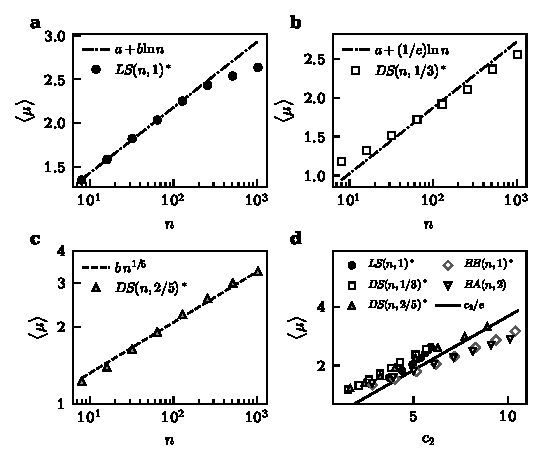
\includegraphics[width=\linewidth]{figs/fig-mu-random.pdf}
\caption{\textbf{The random baseline.} Average shortest path multiplicity
$\langle\mu\rangle$ against network size $n$ for randomized networks (starred),
which keep each node's degree but destroy all local structure. (a) $LS(n,1)^*$,
degree exponent $\gamma=5$: growth stalls, the points falling away from the
fitted logarithm. (b) $DS(n,1/3)^*$, $\gamma=3$: logarithmic, near the predicted
slope $1/e$. (c) $DS(n,2/5)^*$, $\gamma=5/2$: the predicted power law $n^{1/5}$.
(d) All models, including the non-local $BA(n,2)$, plotted against the excess
degree $c_2$ collapse onto the mean-field line $c_2/e$ of
Eq.~\eqref{eq:path-mf}.}
\label{fig:mu-random}
\end{figure}

The Barab\'asi--Albert model deserves its own note, because it is a
\emph{growing} network yet lands squarely on the random baseline. With $m=2$ it
has $\gamma=3$, and its multiplicity creeps up logarithmically, exactly as its
reshuffled cousins do. It has no local structure to lose: its newcomers attach
across the whole graph and never consult a neighborhood. This echoes the previous
chapter, where the very same model failed to develop communities. Lacking
locality, it builds neither the modules nor the redundant paths, and on both
counts it behaves as though its links had been shuffled at random.

\section{Local rules boost the multiplicity}

Now run the same models \emph{without} shuffling, and compare each against its own
starred baseline (Figure~\ref{fig:mu-local}). The multiplicity climbs decisively
faster. It helps to keep a ladder of growth rates in mind: constant, then
logarithmic, then \emph{log-quadratic}, then \emph{exponential} --- each rung
leaving the one below it far behind.

Most local rules --- local search and the bubble model among them --- sit on the
log-quadratic rung,
\begin{equation}
  \langle\mu\rangle = a + b\ln n + c(\ln n)^2,
  \label{eq:path-typeI}
\end{equation}
the extra squared term bending the curve clearly upward. For $LS(n,1)$ this is a
particularly sharp contrast: the unshuffled network grows without limit while the
shuffled one, with the very same degrees, stops growing altogether. Whatever is
doing the work is not in the degree distribution at all.

The duplication--split rule is different, and dramatically so: its multiplicity
grows \emph{exponentially} with size,
\begin{equation}
  \langle\mu\rangle = a\, e^{bn}, \qquad a,b>0.
  \label{eq:path-typeII}
\end{equation}
Exponential growth is a different world from logarithmic. Over the same range of
sizes in which its shuffled counterpart moves from $\langle\mu\rangle\approx1.2$
to $2.6$, the unshuffled $DS(n,1/3)$ runs from $1.3$ to more than $10^5$: by a
thousand nodes, a typical pair of nodes is joined by hundreds of thousands of
equally short routes. Copying, it turns out, is the great multiplier of shortest
paths, and that is what the title of this chapter names.

\begin{figure}[t]
\centering
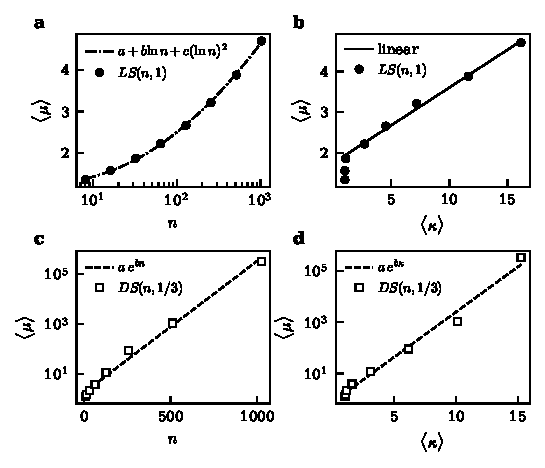
\includegraphics[width=\linewidth]{figs/fig-mu-local.pdf}
\caption{\textbf{Local rules boost the multiplicity.} (a) Local search
$LS(n,1)$ grows log-quadratically, Eq.~\eqref{eq:path-typeI} --- while its
shuffled counterpart, with identical degrees, saturates
(Figure~\ref{fig:mu-random}a). (b) The same data against the inferred number of
communities $\langle\kappa\rangle$: linear. (c) Duplication--split $DS(n,1/3)$
grows exponentially, Eq.~\eqref{eq:path-typeII}; note the linear size axis and
the logarithmic multiplicity axis, and that the vertical scale spans five decades.
(d) Against $\langle\kappa\rangle$: exponential again. Communities are only
detectable beyond the Ramsey size $r_\kappa$, so the leftmost points in (b) and
(d) sit at $\langle\kappa\rangle=1$.}
\label{fig:mu-local}
\end{figure}

\section{Cycles and the boost}

Why should duplication outrun the rest? The answer is in the kind of loop each
rule makes. The triadic-closure rule of the friends chapter closes
\emph{triangles}, loops of length three --- but in a triangle the two nodes
flanking a third are themselves directly linked, so there is still only \emph{one}
shortest route between any pair. A triangle adds cohesion but no extra routes.
Duplication, by contrast, closes \emph{squares}, loops of length four, and a
square is the smallest loop that genuinely offers a choice: its two opposite
corners are two hops apart by \emph{two} different paths, one around each side.
That single observation is the seed of the boost; the box pushes it a little
further, and the takeaway follows.

\begin{figure}[t]
\centering
\begin{adjustbox}{max width=\linewidth}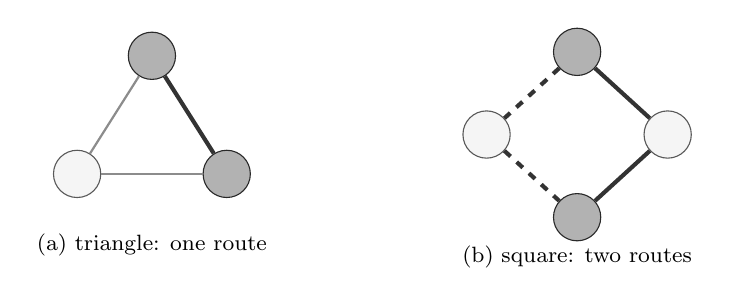
\begin{tikzpicture}[
  nd/.style={circle,draw=black!65,fill=black!4,minimum size=6mm,inner sep=0pt},
  ep/.style={circle,draw=accent!80!black,fill=black!30,minimum size=6mm,inner sep=0pt},
  lnk/.style={draw=black!45,line width=0.8pt},
  r1/.style={draw=black!80,line width=1.5pt},
  r2/.style={draw=black!80,line width=1.5pt,dashed}]
  % panel (a) triangle
  \begin{scope}
    \node[ep] (A) at (0,1.0)    {};
    \node[nd] (B) at (-0.95,-0.5){};
    \node[ep] (C) at (0.95,-0.5){};
    \draw[lnk] (A)--(B);
    \draw[lnk] (B)--(C);
    \draw[r1]  (A)--(C);
    \node[font=\footnotesize] at (0,-1.4) {(a) triangle: one route};
  \end{scope}
  % panel (b) square
  \begin{scope}[xshift=5.4cm]
    \node[ep] (A2) at (0,1.05)   {};
    \node[nd] (B2) at (1.15,0)   {};
    \node[ep] (C2) at (0,-1.05)  {};
    \node[nd] (D2) at (-1.15,0)  {};
    \draw[r1] (A2)--(B2); \draw[r1] (B2)--(C2);
    \draw[r2] (A2)--(D2); \draw[r2] (D2)--(C2);
    \node[font=\footnotesize] at (0,-1.55) {(b) square: two routes};
  \end{scope}
\end{tikzpicture}\end{adjustbox}
\caption{\textbf{Why squares multiply routes.} The two highlighted corners are the
endpoints. (a) In a triangle they are joined directly --- a single shortest route.
(b) In a square they are opposite corners, two steps apart by \emph{two} distinct
routes (drawn solid and dashed), one around each side. Local rules that close
four-cycles, such as gene
duplication, thread the network with these redundant shortest paths.}
\label{fig:path-square}
\end{figure}

Figure~\ref{fig:path-square} makes the contrast concrete.

\begin{calculation}{why copying multiplies routes}
When a node is duplicated, the copy and the original share all their neighbors,
so any two of those neighbors sit at opposite corners of a four-cycle --- each
such pair instantly gains a second shortest route. A duplicated node of degree
$k$ creates $\tbinom{k}{2}=k(k-1)/2$ such squares in a single stroke. Moreover the
duplication rule carries its own preferential attachment, the chance of copying a
node being proportional to its degree, which (as in Chapter~\ref{ch:projects})
builds a heavy-tailed degree distribution with exponent $\gamma=1/q$. Squares are
thus laid down in proportion to $k(k-1)$ --- the very combination that
Eq.~\eqref{eq:path-c2} says controls the multiplicity --- on top of a distribution
with many high-degree nodes. Each round of copying compounds the squares laid down
by the last, and it is this compounding, rather than any one square, that is the
suspected origin of the exponential law, Eq.~\eqref{eq:path-typeII}, though a full
account of it remains open.
\end{calculation}

The lesson of the box is that squares, not triangles, are what multiply shortest
routes. The bubble model lets us test that directly, since it dials the loop
length by hand: a chain of $L$ added nodes makes a loop of length $L+2$. The
geometric intuition survives the test (Figure~\ref{fig:mu-bubble}a). Even-length
loops, whose opposite corners enjoy two equal routes, enrich the network more than
odd ones: $L=2$ and $L=4$ sit well above $L=1$ and $L=3$. But the test also sets a
limit on how much the geometry explains. Every bubble model, whatever its loop
length, stays on the log-quadratic rung. Even loops beat odd ones, and squares
beat triangles --- yet neither buys the exponential. The square-counting explains
why duplication \emph{outruns} triadic closure; the full ferocity of
duplication--split needs the compounding above.

One more clue shows that randomness itself plays a role
(Figure~\ref{fig:mu-bubble}b). The Dorogovtsev--Goltsev--Mendes ``pseudofractal''
network \citep{dorogovtsevgoltsev2002} is a \emph{deterministic} relative of the
bubble model, grown by a fixed clockwork rule rather than a random one: at every
step, new nodes are added to \emph{every} link at once. Its degree distribution is
scale-free with $\gamma = 1+\ln 3/\ln 2\approx 2.6$, so by
Eq.~\eqref{eq:path-power} its randomized version should show a power law with
$\alpha\approx0.16$ --- and it does. The deterministic original, however, grows
only logarithmically: it falls \emph{below} its own shuffled counterpart. So the
speed-up is not a property of the loop geometry alone; a clockwork rule that
closes loops everywhere at once does worse than chance. It is the interplay of
randomness and locality together, not either by itself, that boosts the
multiplicity.

\begin{figure}[t]
\centering
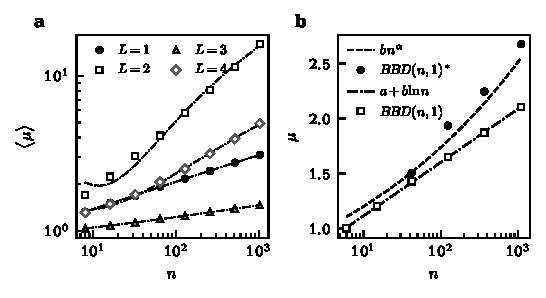
\includegraphics[width=\linewidth]{figs/fig-mu-bubble.pdf}
\caption{\textbf{Cycle length and randomness.} (a) The bubble model $BB(n,L)$,
which closes loops of length $L+2$. Even $L$ (2 and 4) reaches a higher
multiplicity than odd $L$ (1 and 3), as the square-counting predicts --- yet every
$L$ stays log-quadratic, so cycle geometry alone does not buy the exponential.
(b) The deterministic bubble model $BBD(n,1)$ grows only logarithmically, falling
\emph{below} its own randomized version $BBD(n,1)^*$, which follows the power law
of Eq.~\eqref{eq:path-power} with $\alpha\approx0.16$. Locality without randomness
is not enough.}
\label{fig:mu-bubble}
\end{figure}

\section{How fast could it possibly grow?}

If randomness and locality together drive the multiplicity up, it is fair to ask
where the ceiling is. There is one construction for which the question can be
answered exactly, and it is a close relative of the bubble rule: the \emph{diamond
lattice} \citep{migdal1975,kadanoff1976}. Start with a single link joining two
poles $A$ and $B$. At each generation, replace \emph{every} link by two parallel
paths of two links each (Figure~\ref{fig:mu-diamond}a). Where the bubble model
drops one bubble on one randomly chosen link, the diamond drops a bubble on all
links at once, in perfect symmetry.

\begin{calculation}{the multiplicity of the diamond lattice}
The construction is exactly renormalizable, because distinct copies of the
previous generation meet only at their corners. Read it backwards: generation
$G_t$ is two parallel branches, each made of two copies of $G_{t-1}$ in series.
Along a series, lengths add and multiplicities \emph{multiply}; across parallel
branches of equal length, multiplicities \emph{add}. So the pole-to-pole distance
$D_t$ and multiplicity $P_t$ obey
\begin{equation}
  D_t = 2 D_{t-1} = 2^t, \qquad P_t = 2 P_{t-1}^{\,2},
  \label{eq:diamond-rec}
\end{equation}
with $P_0=1$. Taking a logarithm linearizes the recursion and gives
\begin{equation}
  P_t = 2^{\,2^t-1} = 2^{\,D_t-1},
  \label{eq:diamond-pole}
\end{equation}
a \emph{doubly} exponential count. The reason is transparent: a shortest route
must thread $D_t$ successive scales, and at each one it independently picks one of
two parallel branches, so the choices multiply. Averaging over all pairs rather
than the poles alone changes only the prefactor, $\langle\mu\rangle_t \approx
2.1\,P_t/n_t$, since the sum is dominated by near-antipodal pairs. Finally, the
generation carries $n_t = (2\cdot4^t+4)/3$ nodes, so $2^t \simeq \sqrt{3n/2}$, and
substituting into Eq.~\eqref{eq:diamond-pole} turns the doubly exponential in $t$
into a \emph{stretched exponential} in $n$:
\begin{equation}
  \langle\mu\rangle \approx a\,e^{\,b\sqrt{n}},
  \qquad b = \sqrt{\tfrac32}\,\ln 2 \approx 0.849 .
  \label{eq:diamond-n}
\end{equation}
\end{calculation}

The numbers are worth seeing, because they are exact rather than fitted
(Figure~\ref{fig:mu-diamond}b). By the sixth generation the diamond has only
$2732$ nodes, yet an average pair is joined by some $7\times10^{15}$ distinct
shortest paths. This is the fastest growth found anywhere in this chapter, and its
origin is the same parallel branching that the local rules exploit --- only here
it is applied everywhere, at every scale, without a single random choice. Perfect,
maximally symmetric branching therefore sets a hard ceiling on the redundancy a
growing network can carry, and the stochastic local rules of the previous sections
all fall below it.

\begin{figure}[t]
\centering
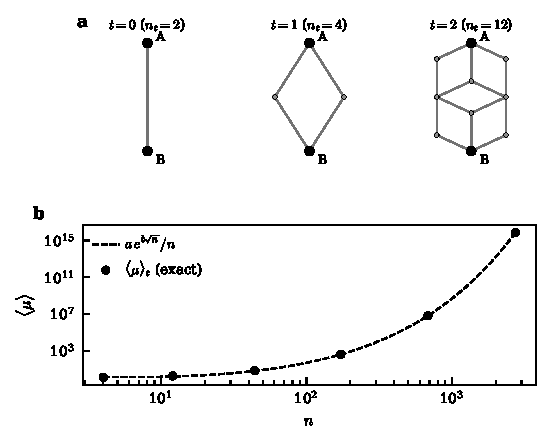
\includegraphics[width=\linewidth]{figs/fig-mu-diamond.pdf}
\caption{\textbf{The exactly solvable ceiling.} (a) The diamond lattice: every
link is replaced, at every generation, by two parallel two-link paths. (b) Its
average multiplicity, computed exactly, follows the stretched exponential of
Eq.~\eqref{eq:diamond-n} across fifteen decades. With $2732$ nodes, a typical pair
of nodes is already joined by some $7\times10^{15}$ equally short routes.}
\label{fig:mu-diamond}
\end{figure}

\section{Two sides of one coin}

Because local rules also create communities, and the number of communities grows
along with the network, we can ask how the multiplicity depends on the number of
communities directly. The relationship is a clean one
(Figure~\ref{fig:mu-local}b and d): linear for every local model tested, and ---
once again the exception --- exponential for duplication--split. This is the
empirical correlation of \citet{deng2026} restated from the inside: more
communities go hand in hand with more shortest paths.

But the point of the chapter is that this partnership is not a case of one
causing the other. ``Local rules boost shortest path multiplicity'' and
``communities accompany high shortest path multiplicity'' are two true statements
about the same networks, and as descriptions they say the same thing. Only one of
them, however, names a \emph{mechanism}. Communities are something an algorithm
reads off a finished network after the fact; the local rule is the process that
actually built that network, node by node, closing the very loops that both carve
it into communities and thread it with redundant routes. Community structure and
path multiplicity are two sides of a single coin --- and the coin is locality.

\section{Real networks}

Models are one thing; the networks we started from are another. Three systems can
be caught at different stages of their growth, which is what we need if we are to
watch $\langle\mu\rangle$ move with $n$ (Figure~\ref{fig:mu-real}). The Internet
at the level of autonomous systems, mapped daily over several years
\citep{snapnets}. The protein interaction networks of a dozen organisms
\citep{stark2006}, which stand in for successive stages of evolution. And the
co-authorship network of the \texttt{cond-mat} preprint archive
\citep{cornellarxiv}, accumulated year by year. In each case we can also compute
the excess degree $c_2$ and so plot the mean-field expectation
$c_2/e$ alongside the measurement --- the random network with the same degrees.
The data are noisy and the systems are not stationary, so no strong claim is
available; but the trends are instructive.

In every system the multiplicity rises with size, and in every system it is
high: the human protein network reaches $\langle\mu\rangle\approx64$, meaning a
typical pair of proteins is joined by some sixty-four equally short chains of
interaction. The protein networks are also the ones that climb
\emph{exponentially} with size, which is the signature of duplication --- and gene
duplication is, of course, exactly how they are thought to grow
(Chapter~\ref{ch:duplication}). The Internet and the co-authorship network both
climb as power laws, more sedately.

The most interesting feature, though, is which side of the mean-field line each
system falls on, because the two disagree in a way that lines up with the degree
correlations of Chapter~\ref{ch:introduction}. The Internet sits \emph{below} its
random expectation: it is \emph{disassortative}, its hubs presiding over
peripheries of poorly connected nodes, and such a star-like arrangement gives a
route no alternatives --- everything must pass through the hub. The co-authorship
network sits \emph{above} it: it is \emph{assortative}, its well-connected authors
writing with one another, and a clique of hubs is exactly what furnishes many
equally short ways across. The same reading applies to the protein networks, which
are disassortative and duly fall below the line. Degree correlations, in other
words, modulate the redundancy on top of what the degrees alone would give ---
a suggestion the mean-field calculation, which knows only $c_2$, cannot yet
account for. It is one of the clearer invitations this book leaves open.

\begin{figure}[t]
\centering
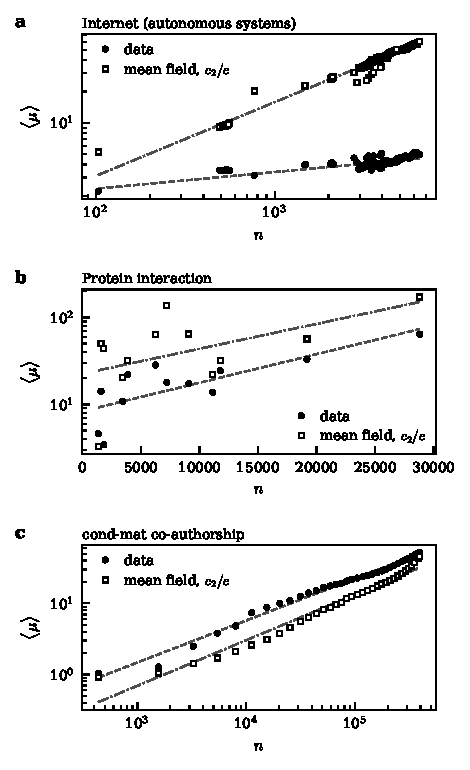
\includegraphics[width=\linewidth]{figs/fig-mu-real.pdf}
\caption{\textbf{Real networks.} Average multiplicity against size, with the
mean-field expectation $c_2/e$ for a random network of the same degrees.
(a) The Internet at the autonomous-system level: a power law, falling below the
random expectation --- the mark of disassortative, star-like wiring. (b) Protein
interaction networks of a dozen organisms: exponential growth, the duplication
signature, reaching $\langle\mu\rangle\approx64$ for the human network. (c)
\texttt{cond-mat} co-authorship: a power law lying \emph{above} the random
expectation, as assortative mixing among prolific authors provides many equally
short routes.}
\label{fig:mu-real}
\end{figure}

\section{Summary}

The shortest paths of real networks are richly redundant, and that redundancy
travels with their community structure. For a random network the redundancy is no
mystery: it is the branching factor, $\langle\mu\rangle\approx c_2/e$, and it
grows only as fast as the hubs allow --- not at all when $\gamma>3$,
logarithmically at $\gamma=3$, as a power law below it. Networks built by local
rules leave that baseline behind, log-quadratically for most rules and
exponentially for duplication, which closes the four-cycles that give opposite
corners two shortest routes apiece. Neither cycle geometry nor locality is
sufficient by itself: a deterministic rule that closes loops everywhere at once
does worse than chance, while the perfectly symmetric diamond lattice, where the
branching can be solved exactly, marks the ceiling at a stretched exponential.
Since the same local rules also produce the communities, the observed tie between
path multiplicity and communities is best understood not as cause and effect but
as two consequences of one underlying local dynamics.


% instructions
% references
% - https://arxiv.org/abs/2605.25237

% instructions
% references
% - Noh & Rieger, Phys. Rev. Lett. 92, 118701 (2004), mean first passage times
% - Villegas et al., Nature Physics 19, 445 (2023), the Laplacian RG
% - Villegas et al., Phys. Rev. Research 4, 033196 (2022), entropic transitions
% - Rosvall & Bergstrom, PNAS 105, 1118 (2008), the map equation
% - figs/heat_diffusion.py generates every number, table and figure in it

\chapter{Diffusion and the scales it finds}
\label{ch:diffusion}

\section{Diffusion, not just drift}

Chapter~\ref{ch:search} put a walker on a network and used it to \emph{grow} one.
The walker was a device: what mattered was how often it landed on a node, because
that set how fast the node acquired links. This chapter puts a walker on the
networks those rules have already built, and asks what it can tell us about them.
It is the same walk. The question is different, and so is the part of the walk that
answers it.

Start with what a random walk forgets, because Chapter~\ref{ch:search} leaned on it
and it is worth being exact about what was borrowed. On a connected network the walk has a unique stationary
distribution, and it is the one Chapter~\ref{ch:search} used,
\begin{equation}
  P^\infty_i = \frac{k_i}{2m},
  \label{eq:hc-stationary}
\end{equation}
reached from any starting point. That distribution knows the degree sequence and
nothing else: two networks with the same degrees are indistinguishable to it. And
the blindness runs a little deeper than the stationary state. The mean time for a
walker to \emph{return} to where it started is
\begin{equation}
  \langle T_{ii}\rangle = \frac{2m}{k_i},
  \label{eq:hc-return}
\end{equation}
exactly, on every connected network \citep{noh2004} --- an identity with no
architecture in it at all. Whether the node sits in a dense community, on a bridge,
or at the end of a long chain does not enter. Only its degree and the size of the
network do.

It would be easy to conclude from those two identities that a classical walk can
report only degrees, and that conclusion is the one thing this chapter most needs to
head off. What is degree-blind is the walk's \emph{stationary} behaviour --- where it
ends up, and how long it takes to come home. How it gets there is not blind at all,
and everything below is an attempt to read it.

\begin{calculation}{first passage times, and what they know}
Let $\langle T_{ij}\rangle$ be the mean number of steps for a walker started at $i$
to first reach $j$. For a connected undirected network this has a closed form in
terms of $L^{+}$, the Moore--Penrose pseudoinverse of the Laplacian $L=D-A$:
\begin{equation}
  \langle T_{ij}\rangle = 2m\big(L^{+}_{jj} - L^{+}_{ij}\big).
  \label{eq:hc-mfpt}
\end{equation}
Setting $i=j$ recovers Eq.~\eqref{eq:hc-return}. Off the diagonal it does not
simplify, and there is no reason it should: $L^{+}$ is a global object, and
Eq.~\eqref{eq:hc-mfpt} is a statement about how the whole network is wired.

Two cases check the formula, both with elementary closed forms. On the complete
graph $K_n$ every $\langle T_{ij}\rangle=n-1$ for $i\neq j$, and
Eq.~\eqref{eq:hc-mfpt} returns $8.000$ for $K_9$ to fourteen decimal places. On a
ring of $n$ nodes the first passage time to a node $d$ steps away is $d(n-d)$, and
Eq.~\eqref{eq:hc-mfpt} reproduces every value on $C_{21}$ to thirteen.

The asymmetry is where the architecture shows. Unlike the return time,
$\langle T_{ij}\rangle \neq \langle T_{ji}\rangle$ in general, and
\citet{noh2004} showed the difference is a difference of one-node quantities,
\begin{equation}
  \langle T_{ij}\rangle - \langle T_{ji}\rangle = \frac{1}{C_j} - \frac{1}{C_i},
  \label{eq:hc-rwc}
\end{equation}
where $C_i = P^\infty_i/\tau_i$ is the \emph{random-walk centrality}: the
stationary weight of node $i$ divided by its relaxation time. A signal released
everywhere at once reaches the high-$C$ nodes first. Two nodes of equal degree ---
equal stationary weight, equal return time --- can have quite different $C$, and the
difference is exactly the architecture that Eq.~\eqref{eq:hc-return} threw away.
\end{calculation}

So a walk does know more than degrees, provided one watches it before it settles.
The rest of this chapter is about a systematic way to watch it: not at one time, but
at all times at once.

\section{A thermodynamics of diffusion}

\begin{figure}[!ht]
\centering
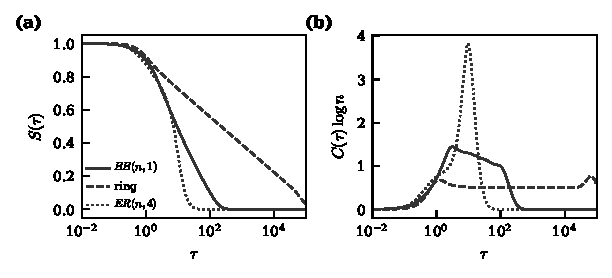
\includegraphics[width=\linewidth]{figs/fig-hc-entropy.pdf}
\caption{\textbf{The diffusion thermometer.} (a) Spectral entropy $S(\tau)$ and
(b) specific heat $C(\tau)\log n$, for a locally grown network, a ring and a random
network of a thousand nodes each. The ring's plateau at $0.5$ is its spectral
dimension of one, read off by Eq.~\eqref{eq:hc-plateau}; the random network's single
peak is its one and only characteristic scale.}
\label{fig:hc-entropy}
\end{figure}

Let a unit of something --- probability, heat, information --- spread over the
network by the diffusion equation $\dot{\mathbf{s}} = -L\mathbf{s}$, whose solution
is the propagator $e^{-\tau L}$. The single parameter $\tau$ is a \emph{diffusion
time}, and it doubles as a resolution: at small $\tau$ the spreading has not left
the immediate neighborhood of wherever it started, at large $\tau$ it has reached
everywhere and forgotten the difference.

The move that turns this into an instrument, due to \citet{villegas2023} and
building on the spectral-entropy formalism of \citet{dedomenico2016}, is to treat
the propagator as a statistical-mechanical density operator,
\begin{equation}
  \rho(\tau) = \frac{e^{-\tau L}}{\mathrm{Tr}\,e^{-\tau L}},
  \label{eq:hc-rho}
\end{equation}
which is the Boltzmann weight $e^{-\beta H}/Z$ with the Laplacian in the role of the
Hamiltonian and the diffusion time in the role of inverse temperature. Everything
statistical mechanics does to a Boltzmann weight can now be done to a network.

\begin{calculation}{entropy, specific heat, and the spectral dimension}
Let $\lambda_1=0\le\lambda_2\le\dots\le\lambda_n$ be the eigenvalues of $L$ and
\begin{equation}
  \mu_i(\tau) = \frac{e^{-\tau\lambda_i}}{\sum_j e^{-\tau\lambda_j}}
  \label{eq:hc-mu}
\end{equation}
the eigenvalues of $\rho(\tau)$. The normalized entropy and its logarithmic
derivative are
\begin{equation}
  S(\tau) = -\frac{1}{\log n}\sum_{i=1}^{n}\mu_i\log\mu_i,
  \qquad
  C(\tau) = -\frac{\mathrm{d}S}{\mathrm{d}\log\tau} .
  \label{eq:hc-SC}
\end{equation}
$S$ runs from $1$ at $\tau=0$, where every node is its own island and $\rho$ is the
identity over $n$, down to $0$ as $\tau\to\infty$, where diffusion has homogenized
everything. $C$ is the specific heat of the diffusion, and it is the quantity to
read, for the reason that makes specific heats useful everywhere else in physics:
\emph{it is flat where nothing is happening and it peaks where a scale is being
crossed}.

The flat value is not arbitrary either. On a structure whose diffusion is governed
by a spectral dimension $d_s$ --- meaning the density of Laplacian eigenvalues near
zero behaves as $\lambda^{d_s/2-1}$ --- the entropy falls logarithmically,
$S \simeq -(d_s/2)\log\tau/\log n + \text{const}$, so that
\begin{equation}
  C(\tau)\,\log n \;\longrightarrow\; \frac{d_s}{2} .
  \label{eq:hc-plateau}
\end{equation}
A constant specific heat is therefore not merely the absence of a scale; its
\emph{height} measures the dimension the diffusion sees. On a ring, $d_s=1$ and the
plateau should sit at $0.5$. Measured on a ring of a thousand nodes it sits at
$0.508$.
\end{calculation}

Figure~\ref{fig:hc-entropy} shows the instrument working on three networks chosen to
bracket the possibilities. The ring gives a broad flat plateau: a walk on a ring
crosses one scale after another with nothing distinguishing them, which is what a
one-dimensional object looks like. The random network gives a single sharp peak: it
has exactly one scale, the crossover from local to global, and once past it there is
nothing left. A locally grown network sits between the two, with a plateau and then
structure.


\section{Two renormalization groups on one lattice}
\label{sec:hc-rg}

\begin{figure}[!ht]
\centering
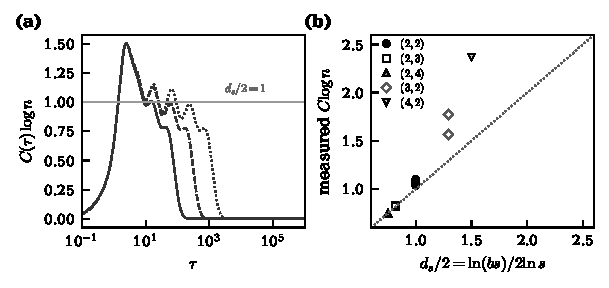
\includegraphics[width=\linewidth]{figs/fig-hc-diamond.pdf}
\caption{\textbf{A renormalization group read off a specific heat.} (a) The diamond
lattice at $b=s=2$ for three generations --- solid, dashed and dotted for $t=4$, $5$
and $6$, that is $n=172$, $684$ and $2732$. Each shows one peak per generation of the
construction, oscillating around the plateau $d_s/2=1$ that
Eq.~\eqref{eq:hc-plateau} predicts, with the ladder lengthening as the lattice
deepens. (b) Measured plateau against the prediction $\ln(bs)/2\ln s$ for the whole
$(b,s)$ family, diagonal dotted. The $b=2$ lattices sit on it; $b\ge3$ has not
converged at the sizes reachable by exact diagonalization.}
\label{fig:hc-diamond}
\end{figure}

On the diamond the instrument stops being descriptive and becomes exact, and the
reason is that this book already has a renormalization group for the same lattice.

Chapter~\ref{ch:communities} built one out of \emph{counting}: collect the block
statistics in a vector, and one generation of the construction acts on them by a
matrix whose two eigenvalues are $\lambda_{\mathrm{vol}}=bs$ for the interiors and
$\lambda_{\mathrm{seam}}=b$ for the boundary, so that the seam fades relative to the
bulk as $1/s$ per generation. That is a renormalization group on the description of
the network. The Laplacian renormalization group of \citet{villegas2023} is a
renormalization group on \emph{diffusion over} it: integrate out the fast modes,
rescale the time, repeat. Two flows, one object. They can be compared, and the
comparison has an answer.

\begin{calculation}{why one step is $s$ and the other is $s^{2}$}
One generation of the $(b,s)$ construction multiplies the pole-to-pole distance by
$s$ and the number of links by $bs$. Because $b$ parallel paths of $s$ links each
replace one link, the two-point resistance is multiplied by $s/b$. Diffusion time on
a resistive network goes as mass times resistance, so
\begin{equation}
  \tau \;\longrightarrow\; (bs)\cdot\frac{s}{b}\,\tau \;=\; s^{2}\,\tau .
  \label{eq:hc-tau-step}
\end{equation}
The walk dimension, defined by $\tau\sim \ell^{\,d_w}$ with $\ell\sim s$ the length
rescaling, is therefore
\begin{equation}
  d_w = \frac{\ln s^{2}}{\ln s} = 2
  \label{eq:hc-dw}
\end{equation}
identically --- for every $b$ and every $s$. The fractal dimension is
$d_f=\ln(bs)/\ln s$, and the spectral dimension follows as
\begin{equation}
  d_s = \frac{2 d_f}{d_w} = \frac{\ln(bs)}{\ln s} .
  \label{eq:hc-ds}
\end{equation}
So the two flows differ by exactly one power. The structural step rescales length by
$s$; the diffusive step rescales time by $s^{2}$, because on this lattice time is
length squared. And the two predictions the next paragraphs test are of different
robustness for a reason now visible: the spacing $s^{2}$ is governed by $d_w=2$,
which is independent of $b$, while the plateau height $d_s/2=\ln(bs)/2\ln s$ grows
with $b$, and a larger spectral dimension needs a larger lattice before its
small-$\lambda$ tail is resolved.
\end{calculation}

Both predictions are borne out, and the caveat the box anticipates is real.

\begin{center}
\footnotesize\setlength{\tabcolsep}{4pt}
\begin{tabular}{lrrrrrr}
\hline
$(b,s)$ & $t$ & $n$ & $d_s/2$ & $C\log n$ & peaks & $\tau$ ratio\\
\hline
$(2,2)$ & $3$ & $44$ & $1.000$ & $1.101$ & $1$ & --- \quad$(s^2{=}4)$\\
$(2,2)$ & $4$ & $172$ & $1.000$ & $1.069$ & $3$ & $4.4$ \quad$(s^2{=}4)$\\
$(2,2)$ & $5$ & $684$ & $1.000$ & $1.051$ & $4$ & $4.4$ \quad$(s^2{=}4)$\\
$(2,2)$ & $6$ & $2732$ & $1.000$ & $1.038$ & $5$ & $4.3$ \quad$(s^2{=}4)$\\
$(2,3)$ & $2$ & $30$ & $0.815$ & $0.824$ & $2$ & $5.3$ \quad$(s^2{=}9)$\\
$(2,3)$ & $3$ & $174$ & $0.815$ & $0.824$ & $3$ & $6.5$ \quad$(s^2{=}9)$\\
$(2,3)$ & $4$ & $1038$ & $0.815$ & $0.823$ & $4$ & $7.2$ \quad$(s^2{=}9)$\\
$(2,4)$ & $2$ & $56$ & $0.750$ & $0.746$ & $2$ & $10.2$ \quad$(s^2{=}16)$\\
$(2,4)$ & $3$ & $440$ & $0.750$ & $0.750$ & $3$ & $12.2$ \quad$(s^2{=}16)$\\
$(3,2)$ & $2$ & $23$ & $1.292$ & --- & $1$ & --- \quad$(s^2{=}4)$\\
$(3,2)$ & $3$ & $131$ & $1.292$ & $1.773$ & $1$ & --- \quad$(s^2{=}4)$\\
$(3,2)$ & $4$ & $779$ & $1.292$ & $1.566$ & $3$ & $4.0$ \quad$(s^2{=}4)$\\
$(4,2)$ & $2$ & $38$ & $1.500$ & --- & $1$ & --- \quad$(s^2{=}4)$\\
$(4,2)$ & $3$ & $294$ & $1.500$ & $2.368$ & $1$ & --- \quad$(s^2{=}4)$\\
\hline
\end{tabular}
\end{center}


\noindent Two kinds of entry are dashed rather than numbered, and neither is a
divergence. A spacing needs two peaks before it is a ratio at all, which is why the
shallowest lattices have none. And the plateau needs a scaling window to average over:
diffusion crosses the whole lattice at $\tau\sim s^{2t}$, so at $t=2$ that happens
before the spreading has escaped the smallest cell, the window closes on itself, and
there is simply no plateau to measure. Both are statements that the lattice is too
shallow to have the structure being looked for, which is the honest thing for the
instrument to say about two generations of anything.

\emph{The ladder.} The specific heat of the diamond is not a single peak
but a sequence of them, one per generation of the construction
(Figure~\ref{fig:hc-diamond}a): at $b=s=2$ there are three peaks at $t=4$, four at
$t=5$, five at $t=6$. A hierarchical lattice built by $t$ nested steps announces all
$t$ of them, at $t$ separate diffusion times. Their spacing converges on
Eq.~\eqref{eq:hc-tau-step} from above for $s=2$ --- $4.43$, $4.39$, $4.30$ against
$s^2=4$ --- and from below for the longer paths, $5.3$, $6.5$, $7.2$ against $9$ at
$s=3$, and $10.2$, $12.2$ against $16$ at $s=4$. The $(3,2)$ lattice at $t=4$ gives
$4.04$ against $4$. The spacing is the robust half of the prediction, as
Eq.~\eqref{eq:hc-dw} says it should be.

\emph{The height.} The plateau the ladder oscillates around is
Eq.~\eqref{eq:hc-plateau}, and for $b=2$ it is confirmed to within one per cent
across three values of $s$: at $(2,2)$ the measured $C\log n$ falls monotonically
through $1.101$, $1.069$, $1.051$, $1.038$ toward the predicted $1.000$ as the
lattice grows; at $(2,3)$ it sits at $0.823$ against a predicted $0.815$; at
$(2,4)$ it hits $0.750$ against a predicted $0.750$. For $b\ge3$ it does not
converge at reachable sizes --- $(3,2)$ reads $1.77$ then $1.57$ against $1.29$,
$(4,2)$ reads $2.37$ against $1.50$ --- moving the right way with size and not
arriving. Those two rows are reported as unconverged rather than as agreement.


The pseudofractal is the control that makes the ladder meaningful. It is built by a
recursion just as deterministic and just as self-similar as the diamond's, and it
has \emph{one} peak, at every generation tested --- $t=4$, $5$ and $6$ alike. There is
no ladder because there is no hierarchy of diffusion times to climb: the
pseudofractal's diameter grows like $\log n$ rather than like a power, so all its
scales collapse into one. Two deterministic self-similar lattices, both in this
book, and diffusion tells them apart at a glance where the community fits of
Chapters~\ref{ch:communities} to~\ref{ch:bubbles} put them in the same class.

\section{What the specific heat does not separate}

\begin{figure}[!ht]
\centering
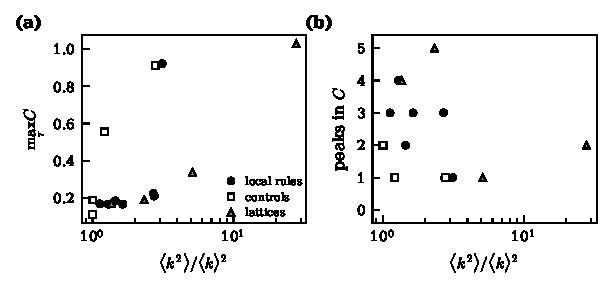
\includegraphics[width=\linewidth]{figs/fig-hc-rules.pdf}
\caption{\textbf{What the specific heat does not separate.} (a) Peak height and
(b) number of peaks against degree heterogeneity, one point per network. Locality
does not order either. The deterministic lattices of the previous section are
the exception.}
\label{fig:hc-rules}
\end{figure}

The diamond is the clean half of the story. Run the same instrument over the
stochastic rules and it is much less impressive, and that has to be said plainly,
because a specific heat is an easy thing to over-read once one has seen it work.

\begin{center}
\footnotesize\setlength{\tabcolsep}{4pt}
\begin{tabular}{lrrrrrr}
\hline
network & $n$ & $\langle k^2\rangle/\langle k\rangle^2$ & $C\log n$ & $\max C$ & peaks & flatness\\
\hline
\multicolumn{7}{l}{\emph{local rules}}\\
\quad $LS(n,1)$ & $1000$ & $1.64$ & $0.85$ & $0.17$ & $3$ & $0.38$\\
\quad $BB(n,1)$ & $1000$ & $2.75$ & $0.85$ & $0.21$ & $1$ & $0.55$\\
\quad $BB(n,2)$ & $1000$ & $1.45$ & $0.91$ & $0.18$ & $2$ & $0.31$\\
\quad $BB(n,3)$ & $1001$ & $1.29$ & $0.90$ & $0.17$ & $4$ & $0.13$\\
\quad $BB(n,5)$ & $1002$ & $1.13$ & $0.85$ & $0.17$ & $3$ & $0.17$\\
\quad $DS(n,0.5)$ & $1000$ & $2.70$ & $0.79$ & $0.22$ & $3$ & $0.71$\\
\quad $DD(n,0.5)$ & $1000$ & $3.13$ & $0.92$ & $0.92$ & $1$ & $1.85$\\
\multicolumn{7}{l}{\emph{controls}}\\
\quad $BA(n,2)$ & $1000$ & $2.79$ & $0.92$ & $0.91$ & $1$ & $1.79$\\
\quad $ER(n,4)$ & $986$ & $1.22$ & $0.87$ & $0.56$ & $1$ & $1.31$\\
\quad ring & $1000$ & $1.00$ & $0.51$ & $0.11$ & $2$ & $0.09$\\
\quad square lattice & $1024$ & $1.01$ & $0.77$ & $0.19$ & $2$ & $0.35$\\
\multicolumn{7}{l}{\emph{deterministic lattices}}\\
\quad pseudofractal & $1095$ & $5.13$ & $0.87$ & $0.34$ & $1$ & $0.98$\\
\quad rec.\ triangle & $768$ & $27.86$ & $0.93$ & $1.03$ & $2$ & $1.81$\\
\quad diamond $(2,2)$ & $2732$ & $2.33$ & $0.89$ & $0.19$ & $5$ & $0.36$\\
\quad diamond $(2,3)$ & $1038$ & $1.36$ & $0.81$ & $0.17$ & $4$ & $0.22$\\
\hline
\end{tabular}
\end{center}


\noindent What the specific heat does \emph{not} do is classify the growth rules. It
does not separate local from non-local: the peak height $\max_\tau C$ runs from
$0.17$ to $0.23$ across the bubble family and $LS(n,1)$, sits at $0.92$ for
duplication--divergence, and sits at $0.91$ for the non-local $BA(n,2)$ ---
duplication and preferential attachment landing on top of each other, which is the
one pairing this book most wants separated. Nor is it simply reading degree
heterogeneity, tempting as that looks: $BB(n,1)$ and $BA(n,2)$ have almost the same
$\langle k^2\rangle/\langle k\rangle^2$, $2.75$ against $2.79$, and differ by a
factor of four in $\max_\tau C$. And no peak of $C$ lands on the mean community size
$\langle n_B\rangle$ of Chapter~\ref{ch:graphons} for any rule, so the hope that a
specific heat would find the community scale for free is not fulfilled.

That is three things $C$ is not, and they are worth the space because the quantity
is easy to over-read. A peak in a specific heat is a scale, but a network may have
scales for reasons that have nothing to do with how it grew --- a broad degree
distribution will manufacture one --- and disentangling those on a stochastic rule is
beyond what this instrument does alone.


\section{Communities as compressed walks}

There is a third way to find communities in this book, and it belongs here rather
than in Chapter~\ref{ch:communities}, because its object is a walk.

Chapters~\ref{ch:communities} to~\ref{ch:bubbles} all minimize a description length,
and they all describe the same thing: the adjacency matrix. The map equation of
\citet{rosvall2008} minimizes one too, but of a \emph{random walk} on the network.
Name the modules, and a walk becomes a sequence of within-module codewords plus an
occasional module switch; a good partition is one that keeps that transcript short,
because the walker rarely leaves a module and so rarely pays for a switch. Compressing
the adjacency matrix asks where the links are; compressing a walk asks where the flow
goes, which depends on the links but also on how they compose into paths.

That gives the book three instruments for one question, and they are ordered by how
much dynamics they contain: the block model, which sees only the counts; the motif
alphabet of Chapter~\ref{ch:motifs}, which sees repeated wiring templates; and the
map equation, which sees where a walk gets stuck. Chapter~\ref{ch:bubbles} argued
that the first two are two currencies for one substance. Does the third buy the same
substance?

\subsection*{A test with a decisive pair}

The question has a clean experiment, because Chapter~\ref{ch:bubbles} supplies two
networks its two currencies treat oppositely. The pseudofractal --- $DBB(n,1)$, the
deterministic triangle rule --- has a footprint that tiles it completely: the alphabet
names $100\%$ of its links, and a fit with that alphabet then reports \emph{no}
communities at any size. Yet its meso-structure total $\kappa_0+\kappa$ still grows in
proportion to $n$, because the motifs are all there and all counted. $BB(n,1)$, the
stochastic version of the same triangle rule, has its footprint overlap itself: the
alphabet names $54\%$, and a genuine community residue is left over.

So the two hypotheses make opposite predictions. If the map equation buys the
meso-structure \emph{total}, it must find modules in both, since that total grows like
$n$ in both. If it buys the community \emph{residue}, it finds them only in the second.

\begin{center}
\footnotesize\setlength{\tabcolsep}{4pt}
\begin{tabular}{lrrrrrr}
\hline
 & & & \multicolumn{4}{c}{modules, by regularization strength}\\
network & $n$ & $m/n$ & none & $0.5$ & $1.0$ & $2.0$\\
\hline
pseudofractal $DBB(n,1)$ & $366$ & $1.99$ & $2$ & $26$ & $\mathbf{1}$ & $1$\\
pseudofractal $DBB(n,1)$ & $1095$ & $2.00$ & $6$ & $61$ & $\mathbf{1}$ & $1$\\
pseudofractal $DBB(n,1)$ & $3282$ & $2.00$ & $15$ & $160$ & $\mathbf{1}$ & $1$\\
diamond $(2,2)$ & $684$ & $1.50$ & $7$ & $45$ & $\mathbf{1}$ & $1$\\
diamond $(2,2)$ & $2732$ & $1.50$ & $12$ & $167$ & $\mathbf{1}$ & $1$\\
$BB(n,1)$ & $400$ & $1.99$ & $4$ & $30$ & $\mathbf{1}$ & $1$\\
$BB(n,1)$ & $1200$ & $2.00$ & $2$ & $81$ & $\mathbf{74}$ & $1$\\
$BB(n,1)$ & $3600$ & $2.00$ & $4$ & $220$ & $\mathbf{221}$ & $1$\\
$BB(n,2)$ & $1200$ & $1.50$ & $3$ & $102$ & $\mathbf{1}$ & $1$\\
$BB(n,2)$ & $3600$ & $1.50$ & $5$ & $283$ & $\mathbf{277}$ & $1$\\
ring $C_n(1)$ & $1200$ & $1.00$ & $5$ & $165$ & $\mathbf{1}$ & $1$\\
ring $C_n(1)$ & $3600$ & $1.00$ & $9$ & $413$ & $\mathbf{1}$ & $1$\\
ring $C_n(1,2)$ & $1200$ & $2.00$ & $4$ & $111$ & $\mathbf{111}$ & $1$\\
ring $C_n(1,2)$ & $3600$ & $2.00$ & $7$ & $291$ & $\mathbf{291}$ & $1$\\
ring $C_n(1,2,3)$ & $1200$ & $3.00$ & $3$ & $88$ & $\mathbf{87}$ & $1$\\
\hline
\end{tabular}
\end{center}


\noindent The residue wins, and not narrowly. On the pseudofractal the map equation
returns a single module at every size tested, up to $n=3282$; on the diamond, the other
lattice the alphabet names completely, the same. On $BB(n,1)$ it returns one module at
$n=400$ and then $74$ and $221$ at $n=1200$ and $3600$ --- a constant density of about
$0.06$ per node once past an onset. $BB(n,2)$ does the same with a later onset. The map
equation is tracking $\kappa$ and not $\kappa_0+\kappa$: it reports nothing on exactly
those networks whose structure a blueprint can stamp out, even though the structure is
demonstrably there.

The rings sharpen that, and they are the control Chapter~\ref{ch:communities} supplies
for free. That chapter proves the ring is split by a block model exactly when its links
outnumber its nodes --- when it carries an extensive number of independent cycles. The
map equation agrees on the ring family: $C_n(1)$, sitting at $m/n=1$, gives one module;
add second neighbours and $C_n(1,2)$ at $m/n=2$ gives $111$ and $291$ modules at $n=1200$
and $3600$; third neighbours keep it there. Two instruments with almost nothing in
common, drawing the same threshold on the same family.

But the pseudofractal also has $m/n \to 2$, and it has no modules. So an excess of links
over nodes is necessary and not sufficient, and the missing ingredient is what the map
equation is actually sensitive to. A walk gets stuck only where there is a
\emph{bottleneck}. The ring's excess links leave long arcs with narrow cuts between
them; the pseudofractal's excess links are triangles, which are structure without being
a barrier to anything, laid over a lattice whose hubs put every node within
$\log n$ steps of every other. Meso-structure and bottleneck are not the same property,
and the map equation is a bottleneck detector wearing a description length.

One caveat has to be stated because the numbers move with it. Infomap here is
regularized, and the regularization strength matters: at $0.5$ every network in the
table fragments, the pseudofractal included, into a few per cent of $n$ modules, and at
$2.0$ every one of them collapses to a single module. The discrimination reported above
exists at strength $1.0$. That value is not chosen to produce it --- it is the library's
default, and the setting under which communities in $BB(n,1)$ were reported in the first
place \citep{vazquezcommunities2025} --- but the finding is a statement about the default
regularization rather than a parameter-free fact, and a reader should hold it that way.

There is a last thing worth noticing, and it belongs to the next chapter as much as
this one. The pseudofractal, on which compressing a walk finds no structure at all, is
the network on which Chapter~\ref{ch:quantum} finds a \emph{quantum} walker more tightly
trapped than anywhere else in this book --- confined to under four nodes. A classical
walker needs a bottleneck to be trapped and there is none; a quantum walker can be
trapped by interference, and the triangles supply that in abundance. The same lattice,
two walkers, opposite verdicts. Which is the sharpest available statement of what the
next chapter adds.

\section{What the classical walker misses}

Two things are now on the table, and the next chapter needs both.

The first is that diffusion is a real instrument. It recovers the spectral dimension
of a ring and of a whole family of hierarchical lattices from nothing but a
spectrum; it counts the generations of a construction; and it does all of that with
no partition to infer, no prior to choose and no vocabulary to fix ---
Chapter~\ref{ch:bubbles}'s objection about description length does not apply to it
at all. That is worth having on its own.

The second is what it costs. A classical walk is \emph{irreversible}: it relaxes,
and Eq.~\eqref{eq:hc-SC} is a statement about how it relaxes. The entropy $S(\tau)$
is monotone, running from one to zero, and once it has reached zero the walk has
forgotten everything, including where it began. Everything this chapter measured is
therefore a property of the \emph{approach} to that forgetting --- how fast, through
what scales, in what order. There is no regime in which a classical walker simply
declines to spread.

Chapter~\ref{ch:quantum} removes exactly that. Replace the diffusion equation with
the Schr\"odinger equation and the evolution becomes unitary: nothing relaxes,
nothing is forgotten, and a walker can be confined for all time rather than merely
delayed. The specific heat of this chapter measures the scales on the way to
equilibrium; the localization volume of the next measures a walker that never gets
there. It is the same operator $L$ in both, which is what makes the pair worth
having.

\section{Summary}

A random walk's stationary distribution knows a network's degrees and nothing else,
and its mean return time $2m/k_i$ is exactly as blind --- but its transient behaviour
is not, and the mean first passage time between two nodes is a global quantity whose
asymmetry defines a centrality that degree cannot see. Treating the diffusion
propagator $e^{-\tau L}$ as a Boltzmann weight turns the diffusion time into a
resolution knob and gives a spectral entropy and a specific heat, where a flat
specific heat means no characteristic scale and its height measures the spectral
dimension the diffusion sees: $0.508$ against an exact $0.5$ on a ring. On the
diamond lattice the instrument becomes exact and meets the renormalization group
Chapter~\ref{ch:communities} built by counting. The two differ by one power, for a
reason that can be derived: the structural flow rescales length by $s$ while the
diffusive flow rescales time by $s^2$, because the walk dimension of this lattice is
two for every $b$ and $s$. The specific heat then shows one peak per generation of
the construction, spaced by $s^2$, oscillating around a plateau at
$\ln(bs)/2\ln s$ --- confirmed to one per cent for $b=2$ across three path lengths,
and unconverged for $b\ge3$. The pseudofractal, self-similar by an equally
deterministic recursion, has one peak and no ladder, because its scales collapse
into a logarithm. What the specific heat does \emph{not} do is classify the
stochastic rules: it puts duplication and preferential attachment on top of each
other, and none of its peaks finds the community size. And a classical walk always
relaxes in the end, so everything here measures the approach to forgetting rather than
any refusal to spread.


% instructions
% references
% - https://doi.org/10.1103/pp6q-n7mx (Boettcher & Porter, Phys. Rev. E 112,
%   L062301, 2025), the paper this chapter answers
% - figs/qwalk_ipr.py generates every number, table and figure in it

\chapter{Localization of quantum walks}
\label{ch:quantum}

\section{A walker that does not forget}

This book opened with a walk. Chapter~\ref{ch:search} put a surfer on a network,
let it step from node to node, and found that the mere act of walking manufactures
preferential attachment: a page reached by many routes is reached often, so it
grows. Everything since has been an elaboration of that idea --- other local rules,
other systems, but always a newcomer that acts on what is near it. It is fitting to
close by putting a walker back on the networks those rules built, and asking what
it finds. The answer turns out to say something the earlier chapters could not say
about the rules themselves.

The walker of Chapter~\ref{ch:search} was classical, and classical walkers forget.
On any connected network a random walk settles, after long enough, into the same
stationary distribution --- each node visited in proportion to its degree, $v_i =
k_i/2m$ --- and it settles there no matter where it started. That is precisely what
made the chapter work: the visiting probability could be treated as a property of
the node, not of the walk's history. It is also a kind of blindness. The stationary
distribution of a random walk knows the degree sequence and nothing else. Two
networks with the same degrees --- one grown by triadic closure, one wired at random
--- look identical to it. A classical walk cannot tell us which rule built the
network it is walking on.

A \emph{quantum} walker does not forget. Replace the diffusion equation with the
Schr\"odinger equation and the evolution becomes unitary: probability is shuffled
between nodes without ever being dissipated, amplitudes interfere, and there is no
stationary distribution to relax into \citep{farhi1998,kempe2003,mulken2011}. Where
a classical walk erases its initial condition, a quantum walk carries it forever.
And because it carries it forever, it can be asked a question a classical walk
cannot answer: \emph{how much of the network did the walker ever reach?}

That question has a sharp answer, and the answer, it turns out, is a fingerprint of
the growth rule. This chapter is about measuring it.

The immediate provocation is a paper of \citet{boettcher2025localization}, who put
continuous-time quantum walks on networks built by recursively attaching triangles
and found the walker trapped: confined for all time to a handful of nodes around
where it started. They found the same in two other highly clustered constructions
and concluded that local clustering induces localization. Their networks are close
cousins of the pseudofractal web of Chapters~\ref{ch:communities}
and~\ref{ch:motifs}, and their triangles are the triangles of
Chapter~\ref{ch:friends}, so the result reads like a statement about this book. It
nearly is. What the measurements below show is that clustering is the wrong
variable --- that it is a correlate of the effect and not its cause --- and that the
right variable is one this book already has a name for.

\section{The measure of confinement}

Fix a network of $n$ nodes with adjacency matrix $A$, degrees $k_i$, and let $D$ be
the diagonal matrix of degrees. The walker's state is a complex amplitude on every
node, $\ket{\psi(t)}$, normalized so that $\braket{\psi|\psi}=1$, and it evolves by
the Schr\"odinger equation
\begin{equation}
  \frac{\mathrm{d}}{\mathrm{d}t}\ket{\psi(t)} = -\mathrm{i}\,H\ket{\psi(t)},
  \qquad
  H = D^{-1/2}\big(D-A\big)D^{-1/2},
  \label{eq:qw-schrodinger}
\end{equation}
whose solution is $\ket{\psi(t)}=e^{-\mathrm{i}Ht}\ket{\psi(0)}$. The generator $H$
is the symmetric normalized Laplacian, the standard choice for walks on networks
\citep{faccin2013,boettcher2025localization} and the one whose \emph{ground state}
reproduces the classical stationary distribution, so that the quantum and classical
walkers agree about where a walker at rest should be found and disagree only about
motion. The probability of finding a walker that started at node $j$ on node $i$ at
time $t$ is
\begin{equation}
  \pi_{ij}(t) = \big|\bra{i}e^{-\mathrm{i}Ht}\ket{j}\big|^2 .
  \label{eq:qw-prob}
\end{equation}

How spread out is that distribution? The standard instrument, borrowed from the
theory of electrons in disordered solids \citep{thouless1974,wegner1980}, is the
\emph{inverse participation ratio}
\begin{equation}
  \mathrm{IPR}_j(t) = \sum_{i=1}^{n} \pi_{ij}(t)^2 ,
  \label{eq:qw-ipr}
\end{equation}
and it is easiest to read through its reciprocal. If the walker's probability is
spread evenly over $\ell$ nodes and is zero on the rest, then each of those $\ell$
nodes carries $\pi=1/\ell$ and Eq.~\eqref{eq:qw-ipr} gives
$\mathrm{IPR}=\ell\cdot(1/\ell)^2 = 1/\ell$. So
\begin{equation}
  \ell \;=\; \frac{1}{\mathrm{IPR}}
  \label{eq:qw-ell}
\end{equation}
is the \emph{localization volume}: the effective number of nodes the walker
occupies, counted in a way that does not care how the probability is distributed
among them. Its two extremes bracket everything that follows. A walker pinned to a
single node has $\ell=1$. A walker spread uniformly over the whole network has
$\ell=n$.

That contrast is the whole measurement, and it is a statement about how $\ell$
depends on $n$. A walk is \emph{delocalized} if $\ell$ grows in proportion to the
network --- the walker occupies a fixed \emph{fraction} of a growing system, so it
explores everything. It is \emph{localized} if $\ell$ approaches a constant --- the
walker occupies a fixed \emph{number} of nodes however large the network becomes,
so the fraction it explores goes to zero. There is no need for a threshold value of
the IPR to separate the two cases, which is fortunate, because no natural one
exists \citep{boettcher2025localization}. One only has to grow the network and see
whether $\ell$ moves.

Because the evolution is unitary, $\mathrm{IPR}_j(t)$ never settles down; it
oscillates forever. The quantity to compare across networks is therefore its
long-time mean, $\overline{\mathrm{IPR}_j} = \lim_{T\to\infty}T^{-1}\int_0^T
\mathrm{IPR}_j(t)\,\mathrm{d}t$, which does converge, and which can be written in
closed form. The form is worth seeing once, because it identifies what a network
must supply in order to trap a walker.

\begin{calculation}{the long-time mean, and what makes it large}
Expand in the eigenbasis of $H$, writing $He_m = \lambda_m e_m$. Then
\begin{equation}
  \pi_{ij}(t) = \sum_m A_m^{ij} + \sum_{m<\,n} B_{mn}^{ij}
               \cos\!\big[(\lambda_m-\lambda_n)t\big],
  \label{eq:qw-pi-expand}
\end{equation}
with $A_m^{ij}=|\braket{i|e_m}\braket{e_m|j}|^2$ and
$B_{mn}^{ij}=2\braket{i|e_m}\braket{e_m|j}\braket{j|e_n}\braket{e_n|i}$. Averaging
over time kills every oscillating term whose frequency is nonzero, so
\begin{equation}
  \bar\pi_{ij} = \sum_m A_m^{ij}
    + \sum_{\substack{m<n\\ \lambda_m=\lambda_n}} B_{mn}^{ij} .
  \label{eq:qw-pibar}
\end{equation}
Squaring Eq.~\eqref{eq:qw-pi-expand} before averaging keeps more: a product of two
cosines survives whenever the four eigenvalues involved satisfy
$\lambda_m-\lambda_n=\lambda_s-\lambda_r$, which happens for degenerate pairs and
for \emph{quartets} with matching spacings \citep{boettcher2025localization}.

The lesson does not depend on writing the quartet sums out. A large long-time IPR
requires a network whose Hamiltonian has \emph{degenerate eigenvalues}, or at least
many coincident gaps, because those are the terms that do not average away.
Degeneracy, in turn, is what symmetry produces. So a rule that builds symmetric
local structure --- the same small configuration, over and over --- is a rule that
manufactures exactly the spectral coincidences the walker needs in order to stay
put. This is the thread that Section~\ref{sec:qw-twins} pulls hardest.
\end{calculation}

Everything reported below is a numerical time-average of Eq.~\eqref{eq:qw-ipr} over
a late window, $t\in[400,800]$, sampled at $240$ points, for $24$ start nodes $j$
drawn at random from each network and averaged over them; the walk itself is
computed exactly, by diagonalizing $H$ and phasing its eigenbasis, so the only
approximation is the finite window. Widening the window to $t\in[1600,3200]$ moves
no value reported here by more than about seven percent, and reverses none of the
comparisons. Each stochastic rule is grown ten times at each size. The rules are
the generators of Chapters~\ref{ch:communities} to~\ref{ch:bubbles}, imported
unchanged, so that the networks walked on here are the same networks those chapters
fitted.

\section{Every local rule traps the walker}
\label{sec:qw-flat}

Figure~\ref{fig:qw-density} shows the phenomenon before any averaging. On the left,
a walker started on a network grown by $BB(n,1)$ --- lay a new node across a random
link, closing a triangle --- and left to run. It does not go anywhere. The
probability sloshes back and forth among a few nodes near the start, and the rest of
the network --- three decades fainter --- never fills in, for as long as one cares to
watch. On the right, the same
walker on a ring of the same size, spreading ballistically outward as one would
expect of a wave.

\begin{figure}[t]
\centering
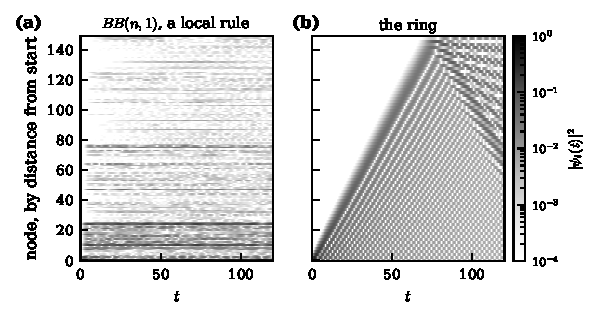
\includegraphics[width=\linewidth]{figs/fig-qw-density.pdf}
\caption{\textbf{A walker that stays, and a walker that goes.} Probability
$|\psi_i(t)|^2$ against node and time, for a walk started on a single node, with
nodes ordered by their distance from that node so that spreading appears as
widening. (a) On $BB(n,1)$, $n=150$, the walker never leaves a neighborhood of its
starting point. (b) On a ring of $150$ nodes it moves away at constant speed and
wraps around. Darker is more probable; the color scale is logarithmic, because a
linear one that resolves the trapped walker leaves the ring almost blank.}
\label{fig:qw-density}
\end{figure}

\begin{center}
\footnotesize\setlength{\tabcolsep}{3pt}
\begin{tabular}{llrrrrrrr}
\hline
 & & & & \multicolumn{4}{c}{$\ell=1/\overline{\mathrm{IPR}}$} & \\
rule & motif & $\langle c\rangle$ & $\langle k\rangle$ & $100$ & $200$ & $400$ & $800$ & $\langle n_B\rangle$\\
\hline
$LS(n,1)$ & \ngon{3} & $0.69$ & $4.0$ & $13$ & $15$ & $14$ & $16$ & $29$\\
$BB(n,1)$ & \ngon{3} & $0.74$ & $4.0$ & $11$ & $13$ & $13$ & $13$ & $34$\\
$BB(n,2)$ & \ngon{4} & $0.00$ & $3.0$ & $11$ & $13$ & $15$ & $14$ & $69$\\
$BB(n,3)$ & \ngon{5} & $0.00$ & $2.7$ & $20$ & $26$ & $28$ & $28$ & $120$\\
$BB(n,4)$ & \ngon{6} & $0.00$ & $2.5$ & $19$ & $22$ & $25$ & $26$ & $304$\\
$BB(n,5)$ & \ngon{7} & $0.00$ & $2.4$ & $31$ & $36$ & $44$ & $45$ & $271$\\
$BB(n,6)$ & \ngon{8} & $0.00$ & $2.3$ & $22$ & $28$ & $35$ & $38$ & ---\\
$DS(n,1/3)$ & \ngon{4} & $0.00$ & $3.7$ & $16$ & $18$ & $19$ & $20$ & $55$\\
$DS(n,0.5)$ & \ngon{4} & $0.00$ & $7.3$ & $8$ & $9$ & $11$ & $10$ & $20$\\
$DD(n,0.5)$ & $K_{2,d}$ & $0.00$ & $7.8$ & $5$ & $5$ & $6$ & $6$ & $26$\\
$BB(n,2)+$ a link & \sqstub & $0.00$ & $4.0$ & $17$ & $21$ & $23$ & $34$ & ---\\
$BB(n,2)+$ a diagonal & \sqdiag & $0.68$ & $4.0$ & $14$ & $16$ & $17$ & $16$ & ---\\
$BA(n,2)$ & --- & $0.03$ & $4.0$ & $25$ & $27$ & $32$ & $32$ & ---\\
$ER(n,4)$ & --- & $0.00$ & $4.1$ & $40$ & $74$ & $152$ & $213$ & ---\\
ring & --- & $0.00$ & $2.0$ & $34$ & $70$ & $140$ & $265$ & ---\\
\hline
\end{tabular}
\end{center}


The table above --- and the left panel of Figure~\ref{fig:qw-scaling} --- turns the
picture into numbers, and what to read is which rows move with $n$ and which do not.
For the ring, $\ell$ doubles as $n$ doubles: $34$, $70$, $140$, $265$, dead on
proportionality across an eightfold range of size. For a random network of the same
kind of sparsity it does much the same, $40$ to $213$. For $BB(n,1)$ it goes $11$,
$13$, $13$, $13$; for $BB(n,2)$, $11$, $13$, $15$, $14$; for $DD(n,0.5)$, $5$, $5$,
$6$, $6$. Those have stopped.

Not every local rule has stopped by $n=800$, and the table says so. The rules with
the largest footprints are still creeping upward at the last size measured ---
$BB(n,5)$ runs $31$ to $45$, $BB(n,6)$ runs $22$ to $38$ --- and it would be
overreaching to call those converged. They do not, in fact, converge:
Section~\ref{sec:qw-exponent} shows that they creep on logarithmically, which is a
weaker statement than saturation and a far weaker one than delocalization. Section~\ref{sec:qw-exponent} comes back to
them with five octaves instead of three and decides between the three things $\ell$
could be doing; for now, what is unambiguous is the comparison, and it is cleanest in
the fraction $\ell/n$, the share of the network the walker actually occupies. For the ring that fraction is $0.35$, $0.35$, $0.35$, $0.33$: constant, as
delocalization requires. For $BB(n,6)$, the slowest-saturating local rule in the
table, it is $0.22$, $0.14$, $0.09$, $0.05$ --- down by a factor of four and a half
while the network grew by eight. Every local rule in the book behaves that way. A
walker put on one of them explores a share of the network that goes to zero; a
walker on a ring or a random network does not.

That is the chapter's first result and it is worth stating plainly. \emph{Networks
grown by local rules localize quantum walks; networks with no local rule do not.}
It is the same dichotomy the book has drawn a half-dozen times --- local rules
produce clustering, hierarchy, correlations, communities, path redundancy, and
non-local ones do not --- appearing now in a dynamical quantity that nobody grew the
networks to have.

One control needs disarming before any of this can be pinned on locality.
$BA(n,2)$, the preferential-attachment model Chapter~\ref{ch:communities} used as its
non-local benchmark, also has a roughly constant $\ell$, around $32$. But the
mechanism there is known and is not ours: a quantum walk on a scale-free network
localizes on the \emph{hubs}, because a node of very high degree is a deep well in
$H$ \citep{faccin2013}. That is a degree effect, present whenever the degree
distribution is broad, and it is the same nuisance the degree-corrected fits of
Chapter~\ref{ch:communities} were introduced to suppress. Two things keep it from
doing the work below. It is weak --- $BA(n,2)$ is the \emph{least} localized of the
broad-degree rules in the table, at more than twice $BB(n,1)$'s $\ell$ --- and the
comparisons that follow are all made between rules whose degree distributions are
comparably broad, several of them at identical mean degree.

\begin{figure}[t]
\centering
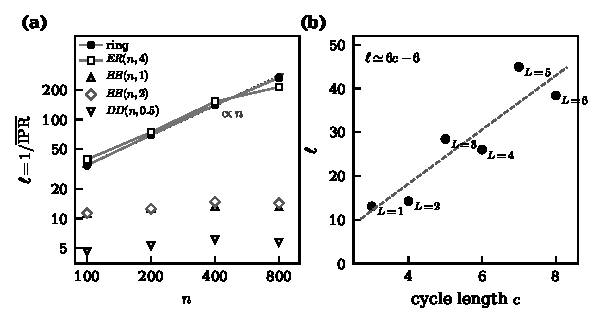
\includegraphics[width=\linewidth]{figs/fig-qw-scaling.pdf}
\caption{\textbf{Localized and delocalized.} (a) The localization volume
$\ell=1/\overline{\mathrm{IPR}}$ against size. The ring and the random network
(lines) grow in proportion to $n$, the dotted line showing that slope; the local
rules (markers) flatten, which is what localization means. (b) For the bubble family
$BB(n,L)$ at $n=800$, $\ell$ against the length $c=L+2$ of the cycle the rule
closes. The dashed line is a least-squares fit. The walker's territory is the size
of the rule's own footprint.}
\label{fig:qw-scaling}
\end{figure}

\section{It is not the clustering}
\label{sec:qw-clustering}

The natural reading of those numbers is the one
\citet{boettcher2025localization} give: these rules make triangles, triangles make
cliquish neighborhoods, and a cliquish neighborhood is a box the walker cannot get
out of. The table refutes it in a single comparison, and the comparison is available
only because Chapter~\ref{ch:bubbles} built the family that makes it.

$BB(n,1)$ and $BB(n,2)$ are the same rule. Both lay a chain of $L$ new nodes across
a randomly chosen link; the only difference is the length of the chain, $L=1$ or
$L=2$, and therefore the length of the cycle it closes, a triangle or a square.
$BB(n,1)$ has a mean clustering coefficient of $0.74$. $BB(n,2)$ has, exactly and by
construction, none at all: it is bipartite, and a bipartite network contains no
triangle whatsoever. Their localization volumes are the same, $13$ and $14$ at
$n=800$.

Zero triangles, identical trapping. Whatever confines the walker on $BB(n,1)$ is
still there when the triangles are removed, so it was never the triangles.

The wider view (Figure~\ref{fig:qw-tests}a) says the same less sharply but more
completely: across the rules of this book, $\ell$ and $\langle c\rangle$ are simply
unrelated. Rules with $\langle c\rangle$ identically zero span the entire range of
localization, from $DD(n,0.5)$ at $\ell\approx6$ --- the most tightly confined
random rule in the table --- to the ring, which is not confined at all. Rules with high
clustering are scattered through the middle. There is no monotone relationship to
find, and no amount of clustering is either necessary or sufficient.

Why, then, did clustering look like the answer? Because
\citet{boettcher2025localization} varied it in constructions where it was
confounded. Their recursive triangle web, the pseudofractal, Holme--Kim and the
Kleinberg model all raise clustering by \emph{adding short cycles}, and one cannot
add a triangle without also adding the shortest cycle there is. Turning up the
clustering knob in all four of their models turns up something else at the same
time, and Section~\ref{sec:qw-footprint} argues it is the something else that
matters. Their own numbers already order themselves that way: reading their figures
against the cycles their rules close rather than against clustering reproduces the
ranking of their curves.

\section{It is not the communities either}
\label{sec:qw-communities}

The next hypothesis is more attractive, and it is the one this book invites. The
localization volume is a number of nodes; communities are groups of nodes; and
Chapter~\ref{ch:graphons} showed that the rules here have a constant \emph{density}
of communities, so that mean community size $\langle n_B\rangle$ is a
size-independent number each rule owns --- exactly the sort of thing a
size-independent $\ell$ might be. On this reading the walker is confined to the
community it was born in, held there by the same faint seam that lets a block model
find the partition at all: Chapter~\ref{ch:communities} proved that the diamond's
boundary decays relative to its interiors like
$\lambda_{\mathrm{seam}}/\lambda_{\mathrm{vol}}=1/s$, and a boundary that fades is a
barrier the walker cannot tunnel through.

It is a good hypothesis. It is wrong, and the instrument that refutes it is again
one the book already built.

Chapter~\ref{ch:bubbles} needed two controls that closed the same square as
$BB(n,2)$ but differed in whether the resulting network had communities: $BB(n,2)$
itself has \emph{no communities at any size}, while adding one further link per step
--- either a link to a neighbor of the far endpoint, which keeps the network
bipartite, or the square's own diagonal, which does not --- puts both variants into
the constant-density class. Same rule, same motif, community structure switched on
and off. Figure~\ref{fig:qw-tests}b walks on all three.

The rule with no communities is the \emph{most strongly} localized of the three:
$\ell=14$ at $n=800$, against $34$ for the variant that adds a link and $16$ for the
one that adds a diagonal. All three sit at the same mean degree, $4.0$, so there is
nothing to blame on density. If communities were the trap, the network with none
could not be the one that traps hardest.

The quantitative check fails too. Across the whole table, $\ell$ never comes close to
$\langle n_B\rangle$ --- it is two to twelve times smaller everywhere --- and the two
do not even agree on the ordering: $BB(n,4)$ has the largest mean community of any
rule measured, $\langle n_B\rangle=304$, and a localization volume of $26$, smaller
than $BB(n,5)$'s $45$ at $\langle n_B\rangle=271$. The walker is not confined to a
community. It is confined to something several times smaller, and to something the
block model is not looking at.

And yet the failure has a shape, and it is a shape the book has already explained.
Look at \emph{which} rule the community hypothesis got wrong. $BB(n,2)$ reports no
communities because Chapter~\ref{ch:motifs} showed that an alphabet containing the
square books its structure as planted motifs instead --- and
Chapter~\ref{ch:bubbles} then showed that this is not a network changing but a
description changing dialect. The meso-structure did not go anywhere; it was
renamed. A rule whose footprint tiles the network cleanly spends its whole
meso-structure budget on motifs and reports no communities; a rule whose footprint
overlaps itself has a remainder, and the remainder is what gets bought at the
bespoke rate and counted as a community. What does not move, across the parity
alternation that sends $\kappa$ from $n^{0.25}$ to $n^{0.93}$, is the total
$\kappa_0+\kappa$.

If that is right, then the community hypothesis was not so much wrong as quoted in
the wrong currency. The walker is not doing inference and cannot see which dialect a
statistician chose; it responds to what is physically there. So it should be
measuring the invariant --- the meso-structure --- and not the residue that the
vocabulary happens to leave in community form. The next two sections test that, and
it is the reading that survives.

\begin{figure}[t]
\centering
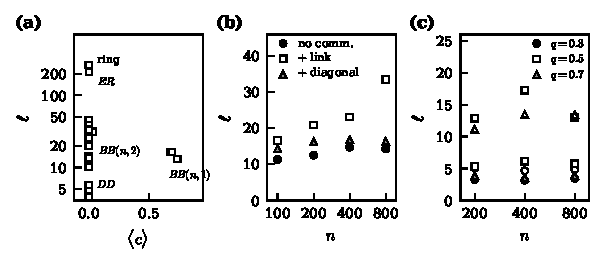
\includegraphics[width=\linewidth]{figs/fig-qw-tests.pdf}
\caption{\textbf{Three tests, two negative.} (a) $\ell$ against mean clustering at
$n=800$, one point per rule: no relationship. $BB(n,1)$ and $BB(n,2)$ are the same
rule at chain length $1$ and $2$ and localize identically, though one is built of
triangles and the other contains none. (b) The same square-closing rule with its
community structure switched on: $BB(n,2)$ has no communities at any size, the two
variants have a constant density of them, and the one with none localizes hardest.
(c) Duplication--divergence with and without its exact symmetries: filled markers as
grown, hollow markers with each class of identical-neighborhood twins collapsed to
one representative. The more of the network is exactly symmetric, the more of the
trapping is destroyed by removing the symmetry.}
\label{fig:qw-tests}
\end{figure}

\section{The volume is the footprint}
\label{sec:qw-footprint}

Return to the bubble family and read it as a family. $BB(n,L)$ closes a cycle of
length $c=L+2$, and $L$ is a dial that changes nothing else about the rule: the same
random link is chosen, the same chain is laid across it, only longer. Turning that
dial moves the localization volume, and moves it in the one way that makes sense
(Figure~\ref{fig:qw-scaling}b). A triangle-closing rule confines the walker to
about a dozen nodes. A rule closing a seven-cycle confines it to about forty-five.
The relation across the family is linear in the cycle length,
\begin{equation}
  \ell \;\simeq\; 6c - 6 ,
  \label{eq:qw-footprint}
\end{equation}
with the parity zig-zag familiar from Chapter~\ref{ch:bubbles} riding on top of it.

So the walker's territory is set by the size of the structure the rule keeps
building. Not by how cliquish that structure is --- the $c=3$ and $c=4$ members
differ by everything in clustering and by nothing in $\ell$ --- and not by how the
structures group themselves into communities, but by the plain linear size of the
rule's own footprint.

One confound has to be cleared before that reading is safe, because within the bubble
family the footprint is not quite the only thing $L$ changes. A step of $BB(n,L)$ adds
$L$ nodes and $L+1$ links, so the mean degree is $\langle k\rangle = 2(L+1)/L$ and
falls as the cycle lengthens, from $4$ at $L=1$ to $2.3$ at $L=6$. Longer footprints
therefore come with sparser networks, and one could ask whether
Eq.~\eqref{eq:qw-footprint} is a statement about cycles or merely about density.

It is about cycles, and the table settles it because several of its rows sit at
\emph{identical} mean degree. $BB(n,1)$, both $BB(n,2)$ variants, $LS(n,1)$ and
$BA(n,2)$ all have $\langle k\rangle=4.0$ to the precision quoted, and their
localization volumes run from $13$ to $34$ --- a spread of two and a half, at fixed
density. In the other direction, $BB(n,2)$ and the $(2,2)$ diamond both have
$\langle k\rangle\approx3.0$ and differ in $\ell$ by a factor of three. Density
matters, as it must, since a walker on a sparser network has fewer directions to go;
but it does not order these rules, and it cannot account for either of those spreads.

The deterministic lattices then confirm the reading with a second, independent dial,
and they matter because the diamond is the one construction in this book whose
community structure is known exactly rather than fitted.

\begin{center}
\footnotesize\setlength{\tabcolsep}{5pt}
\begin{tabular}{lrrrr}
\hline
lattice & $n$ & $\langle c\rangle$ & $\ell$ & $\ell_{\min}$\\
\hline
pseudofractal & $42$ & $0.78$ & $4.2$ & $3.2$\\
 & $123$ & $0.79$ & $3.8$ & $2.5$\\
 & $366$ & $0.80$ & $3.6$ & $2.3$\\
recursive triangle & $48$ & $0.78$ & $6.9$ & $2.7$\\
 & $96$ & $0.78$ & $7.9$ & $3.3$\\
 & $192$ & $0.78$ & $10.5$ & $3.8$\\
 & $384$ & $0.78$ & $12.3$ & $3.2$\\
diamond $(b,s)=(2,2)$ & $44$ & $0.00$ & $4.1$ & $3.4$\\
 & $172$ & $0.00$ & $4.3$ & $3.5$\\
 & $684$ & $0.00$ & $4.2$ & $3.5$\\
diamond $(2,3)$ & $30$ & $0.00$ & $5.9$ & $5.5$\\
 & $174$ & $0.00$ & $7.7$ & $6.4$\\
 & $1038$ & $0.00$ & $7.6$ & $6.4$\\
diamond $(2,4)$ & $56$ & $0.00$ & $8.7$ & $7.8$\\
 & $440$ & $0.00$ & $11.0$ & $9.1$\\
diamond $(3,2)$ & $23$ & $0.00$ & $2.5$ & $2.2$\\
 & $131$ & $0.00$ & $2.6$ & $2.2$\\
 & $779$ & $0.00$ & $2.5$ & $2.2$\\
diamond $(4,2)$ & $38$ & $0.00$ & $2.0$ & $1.8$\\
 & $294$ & $0.00$ & $2.0$ & $1.7$\\
\hline
\end{tabular}
\end{center}


The $(b,s)$ diamond replaces every link by $b$ parallel paths of $s$ links, and
Chapter~\ref{ch:communities} showed that the two parameters do quite different jobs:
$b$ sets how many communities there are, $s$ sets how sharply they separate, through
$\lambda_{\mathrm{seam}}/\lambda_{\mathrm{vol}}=1/s$. If the trap were the community
seam, $s$ would be the parameter that matters and larger $s$ --- a fainter seam ---
would mean tighter confinement. It is exactly backwards. Raising $s$ from $2$ to $3$
to $4$ at fixed $b$ \emph{loosens} the trap, from $\ell=4.2$ to $7.6$ to $11.0$,
because $s$ is also the length of the path the walker has to run along inside the
cell. Raising $b$ tightens it --- $4.2$, $2.5$, $2.0$ at $b=2,3,4$ --- because $b$ is
how many ways the cell branches at each junction, and this happens at essentially
fixed mean degree, $3.0$ to $3.4$ across the three. Both readings are geometric.
Neither is about the partition.

And every one of these numbers is flat in size, this time without qualification. The
$(2,2)$ diamond gives $\ell=4.1$ at $44$ nodes and $4.2$ at $684$; the $(2,3)$
diamond gives $7.7$ at $174$ nodes and $7.6$ at $1038$; the $(3,2)$ diamond gives
$2.5$ at $23$ nodes and $2.5$ at $779$. The lattices are the cleanest demonstration
available that $\ell$ is a property of the \emph{rule} rather than of the network the
rule happens to have produced so far, because for a lattice there is only one network
per size and the flatness cannot be an artifact of averaging over an ensemble.

The pseudofractal is the extreme case and it closes the loop with
\citet{boettcher2025localization}. Built entirely of triangles, the shortest cycle
there is, it confines the walker to $3.6$ nodes at $366$ --- the tightest trap of any
triangle rule in this book, and falling, not rising, with size.

Their own recursive triangle web behaves quite differently, and the difference is the
sharpest thing this chapter has to say about their paper. Its mean $\ell$ does not
settle and does not creep: it grows as a power, $\nu=0.46\pm0.05$ over $48$ to $1536$
nodes, close to $\sqrt{n}$ and unmistakably not a constant
(Section~\ref{sec:qw-exponent}). By the criterion of this chapter the average walker
on that lattice is not localized at all.

What is localized is a minority of starting points. The \emph{minimum} over start
nodes, $\ell_{\min}=1/\max_j\overline{\mathrm{IPR}_j}$, sits at about three at every
depth: a few nodes stay pinned onto a handful forever while the rest grow steadily
freer as the lattice grows. That heterogeneity is not a discrepancy with
\citet{boettcher2025localization} --- it is their own Figure~2, where the absolute and
relative gaps between the largest and smallest long-time IPR both widen with depth and
the minimum IPR tends to zero while the maximum stays finite. The two measurements
agree completely, which is the check that this chapter's instrument is theirs.

Where the readings part is what the agreement licenses. They present the lattice as a
demonstration that clustering localizes quantum walks. What it demonstrates is that
clustering localizes \emph{some} walkers on it, on a lattice whose typical walker
spreads over an unboundedly growing territory --- while the pseudofractal, built of the
same triangles by a rule that tiles them without leftovers, localizes every walker on
it at $\nu=-0.04$. Two triangle lattices, opposite verdicts. The triangle is not what
is doing the work.

What does not follow is their conclusion. Their flagship example is the extremum of
the footprint law, not the generic case: they found the tightest trap available
because the triangle is the shortest cycle there is, and then read the choice of
example as a mechanism.

\section{Measured in meso-units}
\label{sec:qw-meso}

The footprint law and Chapter~\ref{ch:bubbles} are two statements about the same
thing, and putting them side by side turns the chapter's negative results into a
positive one.

Chapter~\ref{ch:bubbles} measured, for the bubble family, the density of
meso-structure $b_0 = (\kappa_0+\kappa)/n$ --- motifs plus communities per node,
counted without regard to which vocabulary named them --- and found it to be a
constant of the rule that falls as the motif grows, from $0.38$ per node at $L=1$ to
$0.09$ at $L=5$, simply because a longer cycle uses more links per copy and fewer
copies fit. Its reciprocal $1/b_0$ is therefore the mean size of a meso-unit in
nodes: about $2.6$ nodes at $L=1$, rising to about $11$ at $L=5$.

Now measure the walker's territory in those units instead of in nodes.

\begin{center}
\footnotesize\setlength{\tabcolsep}{5pt}
\begin{tabular}{lrrrr}
\hline
rule & $c$ & $b_0$ & $\ell$ & $\ell\,b_0$\\
\hline
$BB(n,1)$ & $3$ & $0.38$ & $13$ & $5.0$\\
$BB(n,2)$ & $4$ & $0.20$ & $14$ & $2.8$\\
$BB(n,3)$ & $5$ & $0.15$ & $28$ & $4.3$\\
$BB(n,4)$ & $6$ & $0.12$ & $26$ & $3.1$\\
$BB(n,5)$ & $7$ & $0.09$ & $45$ & $4.0$\\
\hline
\end{tabular}
\end{center}


\noindent Across the family $\ell$ itself varies by a factor of three, from about a
dozen nodes to about forty-five, and it varies for the reason
Section~\ref{sec:qw-footprint} gave: the cell is getting bigger. But the walker's
territory measured in \emph{meso-units},
\begin{equation}
  \ell_0 \;=\; \ell\,b_0 ,
  \label{eq:qw-ell0-def}
\end{equation}
barely moves. It is a handful --- between $2.8$ and $5.0$ --- for every rule in the
family, with the same parity alternation riding on it that Chapter~\ref{ch:bubbles}
found in everything else (odd $L$ near $4.4$, even $L$ near $3.0$), and with no trend
in $L$ at all. Where $\ell$ spans a factor of $3.4$ across the family, $\ell_0$ spans
$1.7$, and within a parity class it is constant to a tenth.

That is the result the community hypothesis was reaching for and missing by one
change of units. The walker is confined to a few units of meso-structure. Whether a
statistician, handed the same network, would call those units motifs or communities
is a question about vocabulary that the walker cannot see and does not answer ---
which is exactly why $BB(n,2)$, whose meso-structure is booked entirely as motifs and
which therefore reports no communities at any size, sits on the same line as
$BB(n,3)$, whose meso-structure is booked largely as communities. Two dialects, one
substance, one localization volume per unit of it.

Read this way the chapter is an independent confirmation of Chapter~\ref{ch:bubbles}'s
central claim, arrived at by a route with no description length in it anywhere. That
chapter argued from minimum description length that a motif and a community are the
same object at two scales and that the invariant is their total. Here a quantum
walker, which knows nothing of priors or alphabets or block models, and which was put
on these networks to answer a different question entirely, agrees: it measures the
total, and it measures it in the units the total is denominated in.

\section{How localized, exactly?}
\label{sec:qw-exponent}

Section~\ref{sec:qw-flat} claimed that $\ell$ stops growing, and was careful to say
that the rules with the largest footprints had not visibly stopped by $n=800$. That
caution has to be paid for, because ``stops growing'' is a strong claim and the
obvious alternatives are hard to tell apart over three octaves of size. Three
candidates fit the same data:
\begin{equation}
  \ell \to \text{const}, \qquad
  \ell \sim a + b\ln n, \qquad
  \ell \sim n^{\nu}\ \ (0<\nu<1).
  \label{eq:qw-three}
\end{equation}
The first is localization. The third is something else entirely --- a walker whose
territory grows without bound but more slowly than the network, so that the
\emph{fraction} explored still vanishes. The second sits exactly between them.

The meso-unit picture of Section~\ref{sec:qw-meso} does not merely permit that
question; it answers it, and ties the answer to a number Chapter~\ref{ch:bubbles}
already measured.

\begin{calculation}{the localization exponent is one minus the census exponent}
Write $\ell_0$ for the walker's territory measured in meso-units rather than in nodes
--- the quantity Section~\ref{sec:qw-meso} tabulated as $\ell\,b_0$ --- so that by
definition
\begin{equation}
  \ell = \frac{\ell_0}{b_0}, \qquad b_0 = \frac{\kappa_0+\kappa}{n},
  \label{eq:qw-ell0}
\end{equation}
$b_0$ being the density of meso-structure. Chapter~\ref{ch:graphons} writes the
census as a power of the size and Chapter~\ref{ch:bubbles} measures it for the total,
$\kappa_0+\kappa \sim n^{\beta}$, whence $b_0\sim n^{\beta-1}$. If $\ell_0$ is a
constant of the rule --- which is what Section~\ref{sec:qw-meso} found, to within the
parity alternation --- then
\begin{equation}
  \ell \;\sim\; n^{\,1-\beta}, \qquad\text{that is}\qquad
  \boxed{\ \nu = 1-\beta\ }.
  \label{eq:qw-nu}
\end{equation}
The three cases of Eq.~\eqref{eq:qw-three} are therefore not three hypotheses about
quantum walks. They are the three limit classes of Chapter~\ref{ch:motifs}, read in a
different variable:
\begin{itemize}
  \item $\beta=1$, a constant density of meso-structure, gives $\nu=0$ and a
    localized walker. Every rule in this book is here.
  \item $0<\beta<1$, the \emph{fractal} class --- definable, and empty in
    Chapter~\ref{ch:motifs} --- gives $0<\nu<1$ and a walker whose territory
    grows as a power.
  \item $\beta=1$ with a logarithmic correction, $\kappa_0+\kappa\sim n/\ln n$, gives
    the marginal $\ell\sim\ln n$.
\end{itemize}
Two warnings about Eq.~\eqref{eq:qw-nu}. It fixes the exponent and not the
prefactor: Section~\ref{sec:qw-meso} bounds $\ell_0$ only between about $3$ and $5$,
so the dictionary is good to a factor of $1.7$ in the amplitude. And it assumes
$\ell_0$ does not itself depend on size --- which is exactly the assumption the
logarithmic case violates, since at $\beta=1$ the power vanishes and $\ell$ inherits
whatever $\ell_0(n)$ does. A log, if there is one, comes from $\ell_0$ and not from
$\beta$.
\end{calculation}

Equation~\eqref{eq:qw-nu} turns a vague claim into a prediction with numbers in
it. Chapter~\ref{ch:bubbles}'s fitted $\beta$ for $\kappa_0+\kappa$ runs from $0.94$
to $1.21$ across the book's rules, so $\nu$ should sit at $0$ to within about
$\pm0.2$ for all of them, and at $0.00$ for the deterministic lattices, whose $\beta$
is exactly one.

Deciding this needs a longer lever arm than Section~\ref{sec:qw-flat} used, and one
correction to the method. A fixed averaging window is not safe at large size: a
ballistic walker on a ring of $3200$ nodes has not crossed it by $t=800$, so the
window truncates the delocalized reference and biases every exponent downward. The
measurements here therefore average over $t\in[2n,4n]$, a window that grows with the
system, and run to $n=3200$ for the stochastic rules and to a few thousand nodes for
the lattices. The three candidates of Eq.~\eqref{eq:qw-three} are then fitted to
$\ell(n)$ and compared by corrected Akaike information, which penalizes the two
two-parameter models for their extra freedom, so that ``constant'' has to be beaten
rather than merely tied.

\begin{center}
\footnotesize\setlength{\tabcolsep}{4pt}
\begin{tabular}{lrrrl}
\hline
rule & sizes & $\nu$ & $\Delta\mathrm{AIC}_c$ & best fit\\
\hline
ring & $100$--$3200$ & $0.99\pm0.00$ & $68.2$ & $n^{\nu}$\\
$ER(n,4)$ & $100$--$3200$ & $0.94\pm0.10$ & $5.3$ & $n^{\nu}$\\
$BA(n,2)$ & $100$--$3200$ & $-0.02\pm0.05$ & $4.8$ & constant\\
$BB(n,1)$ & $100$--$3200$ & $0.01\pm0.02$ & $4.8$ & constant\\
$BB(n,2)$ & $100$--$3200$ & $0.08\pm0.03$ & $0.0$ & $\ln n$\\
$BB(n,3)$ & $100$--$3200$ & $0.15\pm0.04$ & $1.3$ & $\ln n$\\
$BB(n,5)$ & $100$--$3200$ & $0.20\pm0.02$ & $5.0$ & $\ln n$\\
$BB(n,6)$ & $100$--$3200$ & $0.20\pm0.04$ & $2.7$ & $\ln n$\\
$LS(n,1)$ & $100$--$3200$ & $0.06\pm0.03$ & $0.6$ & constant\\
$DS(n,0.5)$ & $100$--$3200$ & $-0.04\pm0.05$ & $4.3$ & constant\\
$DD(n,0.5)$ & $100$--$3200$ & $-0.02\pm0.05$ & $4.8$ & constant\\
$BB(n,2)+$ a link & $100$--$3200$ & $0.30\pm0.05$ & $1.7$ & $n^{\nu}$\\
$BB(n,2)+$ a diagonal & $100$--$3200$ & $0.08\pm0.03$ & $0.5$ & $\ln n$\\
pseudofractal & $42$--$1095$ & $-0.04\pm0.02$ & $6.2$ & constant\\
rec.\ triangle & $48$--$1536$ & $0.46\pm0.05$ & $1.8$ & $n^{\nu}$\\
diamond $(2,2)$ & $44$--$2732$ & $-0.00\pm0.01$ & $12.0$ & constant\\
\hline
\end{tabular}
\end{center}


\noindent The answer is not one answer, and the split is the most interesting thing
in the chapter.

The two controls behave exactly as they must, which is the first thing to check: the
ring gives $\nu=0.99\pm0.00$ and the random network $0.94\pm0.10$, both choosing the
power law over a constant by a wide margin. Scaling the window mattered --- under the
fixed window of Section~\ref{sec:qw-flat} the random network read $0.83$, the
truncation biasing it down --- and with that fixed, delocalization is measured at the
value it should have.

\emph{Genuinely localized, $\nu=0$.} Seven rules choose a constant over both
alternatives, and choose it on an instrument built to punish a constant for being
simple. $BB(n,1)$ gives $0.01\pm0.02$; $LS(n,1)$, $0.06\pm0.03$; the two duplication
rules, $-0.04$ and $-0.02$; the pseudofractal, $-0.04\pm0.02$ over nearly five
octaves. The strongest is the $(2,2)$ diamond: $\nu=-0.000\pm0.008$ across $44$ to
$2732$ nodes --- six doublings --- with a constant beating both two-parameter models by
twelve units of corrected Akaike information. That is as clean as a null result gets,
and it comes from a lattice with no ensemble scatter to average away.

\emph{Logarithmic.} Four rules prefer $a+b\ln n$, and they are all the same kind of
rule: the bubble family at long cycles. $BB(n,5)$ runs $29$, $36$, $45$, $50$, $52$,
$60$ across the sweep, monotone, and $\ln n$ beats a constant by five units and beats
the power law too; $BB(n,6)$ and $BB(n,3)$ do the same less emphatically. Their
nominal exponents, $0.15$ to $0.20$, are what a log looks like when a power law is
fitted to it.

This is the loophole the calculation box flagged, and it is worth being plain that it
is a real effect and not noise. At $\beta=1$ the power vanishes and $\ell$ inherits
$\ell_0(n)$; a logarithm therefore says that the walker slowly \emph{acquires}
meso-units as the network grows, at a rate that would take a factor of a thousand in
size to double its territory. Eq.~\eqref{eq:qw-nu} survives it, because the leading
behavior is still $n^{1-\beta}$ with $\beta=1$; what it does not do is predict the
marginal correction, and the correction is there.

Why the long cycles and not the short ones? The bubble rules with long cycles are the
sparsest networks in the table --- $\langle k\rangle$ falls to $2.3$ at $L=6$ --- and
the sparsest are the ones whose footprints only barely overlap. A rule whose cells
interlock tightly gives the walker a hard wall; a rule whose cells are long thin loops
joined at single links gives it a slow leak. That is a plausible story and this
chapter does not test it, which makes it the most concrete thing the chapter leaves
open.

\emph{Unresolved.} Two rules read as power laws and should not be reported as such.
$BB(n,2)+$a link gives $\nu=0.30\pm0.05$, against the $-0.10$ that
Eq.~\eqref{eq:qw-nu} predicts from its measured $\beta=1.10$ --- but its sequence is
not monotone, falling from $31$ at $n=800$ to $29$ at $1600$ before jumping to $49$ at
$3200$, and the largest size carries only two realizations. The honest reading is that
this rule is not measured well enough, not that it is a counterexample. And the
recursive triangle web gives $\nu=0.46\pm0.05$, on which see below.

So the fractal class stays empty. Nothing in this book localizes a walker with a
genuine exponent $0<\nu<1$, which is what Eq.~\eqref{eq:qw-nu} predicts from the fact
that nothing in this book has $\beta<1$. The dictionary holds where it was derived to
hold. What it did not anticipate --- and what a measurement over three octaves could
not have seen --- is that the marginal case comes with a logarithm attached for the
rules with the loosest footprints.

\begin{figure}[t]
\centering
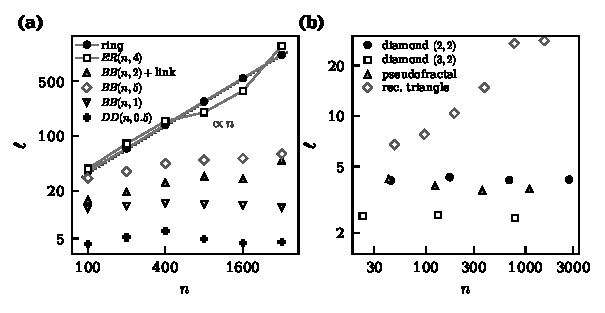
\includegraphics[width=\linewidth]{figs/fig-qw-exponent.pdf}
\caption{\textbf{What $\ell$ does over five octaves.} (a) Stochastic rules and the
two delocalized controls, with the averaging window scaled as $[2n,4n]$ and sizes to
$n=3200$; the dotted line is $\ell\propto n$. (b) The deterministic lattices, which
carry no ensemble scatter and so give the cleanest verdict: one network per size,
nothing averaged over.}
\label{fig:qw-exponent}
\end{figure}

\section{Duplication traps by symmetry}
\label{sec:qw-twins}

One rule in the master table is not explained by any of this, and it is the most
strongly localized of them all. Duplication--divergence, the gene-duplication rule
of Chapter~\ref{ch:duplication}, copies a node and then discards each copied link
with probability $q$. It closes no cycle of fixed length --- its motif is the
biclique $K_{2,d}$, the one motif in the book with no fixed size --- it has no
triangles, and it confines the walker to five nodes, tighter than any bubble rule.

The reason is the one the calculation box in Section~\ref{sec:qw-clustering}
anticipated: duplication does not merely make symmetric structure, it makes
\emph{exact} symmetry, and exact symmetry forces the eigenvalue degeneracies that a
large long-time IPR requires.

\begin{calculation}{why a duplicated node traps a walker}
Call two nodes $u$ and $v$ \emph{twins} if they are not adjacent and have identical
neighborhoods. A duplication step creates a twin outright, and divergence destroys
the relation only if it happens to delete a link, so at any moment a duplication
network carries many twin pairs. Twins have equal degree; call it $k$.

Consider the vector $x$ that is $+1/\sqrt{2k}$ on $u$, $-1/\sqrt{2k}$ on $v$, and
zero elsewhere, and apply $H=D^{-1/2}(D-A)D^{-1/2}$. At a node $i$ adjacent to both
twins,
\begin{equation}
  (Hx)_i = -\sum_j \frac{a_{ij}x_j}{\sqrt{k_ik_j}}
         = -\frac{x_u + x_v}{\sqrt{k_i\,k}} = 0 ,
  \label{eq:qw-twin-nb}
\end{equation}
the two contributions cancelling exactly because the amplitudes are equal and
opposite and the twins have the same degree. At every node adjacent to neither, all
terms vanish. And at $u$ itself the off-diagonal sum runs over $u$'s neighbors,
where $x$ is zero, leaving only the diagonal, so $(Hx)_u = x_u$; likewise at $v$.
Hence
\begin{equation}
  Hx = x ,
  \label{eq:qw-twin-eig}
\end{equation}
an eigenvector at eigenvalue exactly $1$, supported on two nodes, with
$\mathrm{IPR}=1/2$. A twin class of $c$ nodes contributes $c-1$ independent such
vectors, all at the same eigenvalue, so the degeneracy at $\lambda=1$ grows with the
amount of duplication. These are the terms of Eq.~\eqref{eq:qw-pibar} that survive
time-averaging, and they are maximally localized. A walker started on a twin is
partly frozen onto the pair forever.

Numerically the vector is exact --- $\|Hx-x\|$ vanishes to machine precision, and its
IPR is $0.5000$ --- but it accounts for only part of what is there. At $n=400$,
between $39\%$ and $55\%$ of the \emph{entire spectrum} of a $DD(n,q)$ network sits at
exactly $\lambda=1$, and the twins of Eq.~\eqref{eq:qw-twin-eig} force between a
quarter and seven tenths of that, the share rising with $q$. Duplication evidently
produces near-degenerate structure by routes beyond the twin relation --- pendant
nodes hanging off different parents will do it too --- so the theorem is a lower bound
on the degeneracy rather than an account of it. It is enough for the argument, since a
lower bound is all a mechanism needs.
\end{calculation}

Equation~\eqref{eq:qw-twin-eig} is elementary, but it has a consequence worth
spelling out: \emph{duplication localizes quantum walks by an exact theorem, with no
cycles and no clustering anywhere in the argument.} The trap is the symmetry itself.
Nothing about the network's global architecture enters, only the fact that two nodes
are interchangeable.

The prediction is testable by demolition. Take a grown $DD(n,q)$ network, find every
class of twins, and collapse each class to a single representative --- removing the
exact symmetries while leaving the rest of the architecture, the degrees, and the
overall size largely intact. If the twins are doing the trapping, the localization
should largely go away. Figure~\ref{fig:qw-tests}c does it, and the demolition works:
a quarter of the nodes of $DD(n,0.5)$ belong to a twin class, and merging them more
than doubles the localization volume at $n=800$, from $\ell=5.7$ to $13.0$, while the
most extreme confinement --- the walkers frozen with $\overline{\mathrm{IPR}}$ above
$0.7$, that is onto barely more than a single node --- is halved away, to $0.37$.

The strongest form of the test is the dose. Turn $q$, the probability that a copied
link is discarded, and the twin fraction moves with it, because a duplication that
loses no links leaves a perfect twin and one that loses many does not. At $q=0.3$,
$17\%$ of nodes are twinned and merging them costs the trap little, $\ell=3.4$ rising
to $4.8$. At $q=0.5$, $25\%$ are twinned and $\ell$ goes from $5.7$ to $13.0$. At
$q=0.7$, $43\%$ are twinned and $\ell$ goes from $3.9$ to $13.4$, a factor of three
and a half. The more of the network is exactly symmetric, the more of its trapping is
destroyed by removing the symmetry --- which is what a mechanism looks like, as
opposed to a correlation.

This also settles a detail of \citet{boettcher2025localization} that their
clustering account leaves unexplained. Following a walker on their recursive
triangle web, they observe that it ``predominantly alternates between two nodes.''
Two nodes is the signature of Eq.~\eqref{eq:qw-twin-eig}, and their lattice is full
of twins: every generation attaches new nodes across existing links, and two new
nodes laid across the same link are twins by construction. The two-node oscillation
they attribute to clustering is a symmetry, and it is the same symmetry that traps
walkers on protein interaction networks, where the duplication is real and the
triangles are not.

Whether real interactomes show it is a measurement this chapter does not make, and
it is the most concrete thing it leaves open. Duplicate genes are abundant and
long-lived \citep{ohno1970,force1999}, so the twins should be there; but real
divergence is not the independent link deletion of the model, and the question of how
long a twin survives in a genome is exactly the question of how quickly the symmetry
--- and therefore the trap --- decays.

\section{What the walker measures}

Put the three results together and the chapter has found a new kind of instrument.

The localization volume $\ell$ is size-independent, so it is a property of the rule
rather than of the sample. It is set by the footprint of the local rule --- the
length of the cycle closed, the branching of the cell, the exact symmetries a
duplication leaves behind --- and by nothing else the book measures. And it is
\emph{physical}: it is not a statistic computed by fitting a model but a number a
walker on the network produces by moving, and one already measured in the laboratory
on photonic chips \citep{tang2018}.

That last point is worth more than it first appears, because of a difficulty
Chapter~\ref{ch:communities} could not resolve. The Ramsey community number depends
on the method used to detect the communities, and the dependence is not small: on
one and the same network a plain block model and a degree-corrected one disagree by
a factor of twenty-five, and Chapter~\ref{ch:motifs} showed that changing only the
vocabulary can move a rule from having communities at $n=400$ to having none at any
size. A number that moves that much with the observer's choices is an awkward thing
to call a property of a network.

The localization volume has no such freedom. There is no prior to choose, no number
of blocks to infer, no alphabet to fix, no stochastic search that might not have
converged. One diagonalizes a matrix the network hands over and reads off a number.
Where Chapter~\ref{ch:communities} had to build its detection method into the
definition of what it was detecting, the walker just walks.

What it gives up is the partition. $\ell$ says nothing about \emph{which} nodes group
with which --- Section~\ref{sec:qw-communities} was the demonstration that it cannot
--- and it will not hand anyone a list of communities. But
Section~\ref{sec:qw-meso} showed that this is not the same as being blind to the
mesoscale. The walker sees the mesoscale; it simply sees the total rather than the
partition, and it sees the total in whichever dialect the network is actually built
in rather than the one a fit happened to choose. That is precisely the invariant
Chapter~\ref{ch:bubbles} had to reach for description length to isolate, and the two
routes to it could hardly be more different: one an argument about the cheapest way
to transmit a network, the other a wave packet failing to spread. Where they meet is
the best evidence in the book that the invariant is a thing and not an artifact of
how it was found.

There is a prediction in it, and it is easy to state and easy to falsify. If $\ell$
reads the footprint of a network's local rule, then real networks --- whose local
structure Chapter~\ref{ch:introduction} measured and Chapters~\ref{ch:friends}
to~\ref{ch:projects} accounted for --- should have localization volumes of a few
tens of nodes, independent of their size, and social networks built on triadic
closure should sit at the tight end of the range while networks whose local rule
closes longer cycles sit at the loose end. Sharper still: $\ell$ times the density of
meso-structure should come out at a few units, as it does for every rule here, and
Chapter~\ref{ch:graphons} has already measured the community side of that density
across some eighty real networks. Nothing here does the measurement. It is the
obvious next step, the data are the same repositories Chapter~\ref{ch:communities}
used, and the answer would be a statement about the local rule of a real system
obtained without fitting a model to it at all.

\section{Summary}

A classical walker forgets where it started and so can tell us only a network's
degrees; a quantum walker never forgets, and what it remembers turns out to be the
rule that built the network. Measuring the long-time inverse participation ratio on
every growth rule in this book gives a clean dichotomy: on networks grown by a local
rule the walker explores a share of the network that vanishes as it grows, and on a
ring or a random network it does not. Pushed over five octaves of size the dichotomy
resolves into three cases rather than two. Triadic closure, both duplication rules,
the pseudofractal and the diamond genuinely saturate --- the diamond at
$\nu=-0.000\pm0.008$ over six doublings, a constant preferred by twelve units of
Akaike information. The bubble rules at long cycles instead creep on like $\ln n$: a
marginal, log-divergent territory rather than a fixed one. And no rule anywhere shows
a genuine exponent $0<\nu<1$, which is exactly what $\nu=1-\beta$ predicts from the
fact that no rule in this book has $\beta<1$ --- so the fractal limit class of
Chapter~\ref{ch:motifs} is empty on this instrument too. The confinement is not caused by
clustering --- the same rule with its chain length changed from one to two has no
triangles at all and traps just as tightly --- and it is not caused by communities
--- the one square-closing variant with no communities at any size traps hardest of
the three. What sets the localization volume is the linear size of the rule's own
footprint, growing like $6c-8$ in the length $c$ of the cycle closed, tightening
when a deterministic cell branches more and loosening when its paths run longer.
Duplication is a case apart and the sharpest of all: twins are exact automorphisms,
they force eigenvectors of the walk Hamiltonian supported on two nodes, and merging
them triples the walker's territory. The pseudofractal and the recursive triangle
webs that provoked this chapter are then not evidence that clustering localizes
walks; they are the extreme point of the footprint law, the tightest trap available
because the triangle is the shortest cycle there is.

The community hypothesis, in the end, was right about the substance and wrong about
the units. Change the units --- count the walker's territory in the meso-structure of
Chapter~\ref{ch:bubbles} rather than in nodes --- and a localization volume that
varies threefold across the bubble family becomes the same handful of meso-units for
every rule in it, whether the description that network prefers spends its
meso-structure on motifs or on communities. What the walker measures is that
invariant: physically, with no model to fit, no alphabet to fix, and no partition to
infer.


\chapter{Outlook}
\label{ch:outlook}

\section{One principle, many faces}

We have now followed a single idea through six concrete settings, and it is worth
gathering the threads before asking what lies beyond them. In every case the
network grew by a \emph{local} rule --- a newcomer acting only on a node it had
reached and that node's immediate neighbors --- and in every case the same family
of global regularities emerged unbidden.

Searchable networks, such as the citation graph and the World Wide Web, grow by
exploration: a newcomer surfs along links and connects to what it finds. Modeling
the surfer as the very random walk that defines Google's PageRank, we found that a
page's visiting probability rises in a straight line with its in-degree, so that
the local act of walking manufactures an effective ``rich get richer.'' From it
follow a power-law degree distribution whose exponent is fixed purely by how the
network is explored, a clustering hierarchy in which cliquishness falls with
degree, and generically disassortative correlations
(Chapter~\ref{ch:search}).

Social networks grow by introduction: a friend introduces a friend, closing a
triangle. Formalizing the friend-of-a-friend as a \emph{potential link}, born in
proportion to degree, we recovered the same rich-get-richer and the same
clustering hierarchy --- but now with \emph{assortative} correlations, the
well-connected keeping one another's company (Chapter~\ref{ch:friends}). The
contrast with the searchable networks is that chapter's quiet lesson: the sign of
the degree correlations is not a free parameter but a readout of whether the rule
reaches outward, to the periphery, or inward, within a neighborhood.

Biological networks grow by copying: a gene is duplicated, its protein inheriting
all of the ancestor's interactions, and the copies then diverge. Because a node
gains a link whenever one of its neighbors is duplicated, copying too is a
rich-get-richer engine; self-interactions seed the clustering hierarchy, and
coupling divergence to duplication adds a density transition and a multifractal
degree distribution born of inheritance, alongside the disassortative mixing
measured in real protein networks (Chapter~\ref{ch:duplication}). Here the three
mechanisms met in one sentence: a rule that attaches to a \emph{neighbor} of a
randomly chosen node attaches in proportion to degree, because a well-connected
node simply belongs to more neighborhoods. Preferential attachment, the
clustering hierarchy, and the degree correlations are all the generic harvest of
locality.

The same copying, carried into project schedules, refines each activity either by
duplicating it into parallel copies or by splitting it into specialized
sequential parts. The rule predicts identical power laws for an activity's
predecessors and successors, a critical path that vanishes as a fraction of large
projects, and a fractal rather than small-world geometry --- all borne out in
seventy-seven real construction projects --- and it relocates the risk of delay
from the celebrated critical path to a percolation threshold set by the whole
network's average degree (Chapter~\ref{ch:projects}).

Finally, locality proved to shape structure above the level of the individual
node. The same rules that set the degrees also segregate the network into
communities --- even when every node is identical --- a fact we made precise
through the Ramsey community number, the size beyond which communities are all but
certain (Chapter~\ref{ch:communities}); and they thread the network with redundant
shortest paths, multiplying the routes between nodes far faster than chance and in
lockstep with those very communities (Chapter~\ref{ch:distance}).

And with that, the book comes full circle. We set out asking where the global
regularities of real networks come from --- their power-law degrees, their
small-world distances, their clustering hierarchy, their degree correlations ---
and answered, one mechanism at a time, that none of them need be imposed from
above: each emerges from a way of growing in which no node ever uses more than
local knowledge. A node that surfs to a neighbor, befriends a friend, is copied
from an ancestor, or refines a task asks nothing of the network as a whole --- and
yet the networks these humble acts build carry, in the aggregate, the full and
unmistakable signature of real complex systems.

\section{What remains to be done}

If the thesis of this book is right, it opens more questions than it closes.

Several are concrete. The exponential growth of shortest path multiplicity under
the duplication--split rule --- so much faster than the log-quadratic growth of
every other rule we studied --- still wants a full explanation; the
square-counting argument shows why copying outruns triadic closure, but not why it
runs away exponentially. The question is at least better posed than it was, for we
now know what the ceiling is: on the diamond lattice, where the branching can be
solved exactly, the multiplicity grows as a stretched exponential in $\sqrt{n}$,
and every stochastic rule falls below that bound (Chapter~\ref{ch:distance}). What
remains is to explain where between the log-quadratic floor and the deterministic
ceiling a given rule lands, and why copying alone climbs so far.

A second concrete gap sits beside it. The mean-field theory of the multiplicity
knows the network only through its excess degree $c_2$, and that is demonstrably
not enough: real networks fall on either side of the $c_2/e$ line according to the
sign of their degree correlations, the assortative co-authorship graph above it and
the disassortative Internet below. A theory that carries the correlations as well
as the degrees would close the gap between the calculation and the data, and it
would say something the models cannot yet say about which real systems are
route-rich and which are not.

The Ramsey community number has moved further still, though not in the direction
one might have hoped. That it depends on the method used to detect the communities
was always plain. Now that it can be computed exactly, we can say how far that
dependence goes: on one and the same web, under one and the same partition, a
plain block model puts $r_\kappa$ at $1095$ and a degree-corrected one at $42$, and
the two disagree about which cut is best (Chapter~\ref{ch:communities}). The dependence is not a rounding error to be
argued away; it is a factor of twenty-five, and it means a bare Ramsey number
quoted without its detection rule is not a property of the network at all. Yet the
same calculations hand us the beginnings of a repair. Underneath the
method-dependent threshold there is a method-independent quantity: the evidence
density flows to $\ln K$ per link, the entropy of resolving which of $K$
communities a link belongs to, and that value knows nothing of the lattice, the
degrees, or the priors. A definition of emergence built on the invariant rather
than on the crossing --- on the rate at which evidence accumulates rather than on
the size at which it clears an arbitrary bar --- would put the whole idea on firmer
ground.

One question spans both chapters at once, and it may be the most inviting of all.
The ring --- the barest case we can solve, a lattice with no growth and no
randomness in it --- turns out to be split into communities exactly when its links
outnumber its nodes, which is to say exactly when it carries an extensive number of
independent cycles. And cycles are also what multiply its shortest paths. Whether
that accounting is general, or an accident of the ring's simplicity --- whether the
surplus of links over nodes is the common currency of both communities and
redundant routes --- would fold the last two chapters into a single statement. The
book's thesis makes the question natural; it does not answer it.

Two smaller loose ends deserve naming, since both have the flavor of a clue rather
than a nuisance. The number of communities that best describes a self-similar
network appears to grow as $\sqrt{n}$, the geometric midpoint of the network's own
hierarchy --- but that is a numerical observation over the sizes we can reach, not
a theorem, and a proof would be worth having, not least because the same
$\sqrt{n}$ governs the shortest paths on the same lattice. And the Ramsey number's
climb with cycle length carries a persistent even--odd alternation, odd cycles
bringing communities on sooner than the even cycles around them. It is too regular
to be noise and has no explanation.

Even the self-organized critical state of the exhaustive searcher, where a
scale-free network appears across a whole range of the control parameter rather
than at one fine-tuned value, deserves to be connected more tightly to the wider
physics of criticality.

Others are programmatic, and the largest of them is the price we paid for solving
anything exactly at all. Every closed form in the last two chapters --- the ring's
evidence, the diamond's renormalization group, the pseudofractal's counts --- lives
on a \emph{deterministic} lattice, a fixed construction rather than a grown
network, with the candidate partition handed to the calculation rather than found
by an algorithm. That is what made the algebra possible, and it is also the
catch: those results bound and illuminate the simulated ones, but they do not
reproduce them. Whether the renormalization-group map survives off the lattice ---
exactly, or on average, for networks grown at random by a local rule --- sets how
far this reading of emergence extends. It is a demanding question, because on
disordered networks detectability is itself a genuine phase transition, and the
threshold we have been computing would become the edge of a phase rather than the
crossing of a bar. The reward would be a theory of emergence for the networks we
actually care about, rather than for their crystalline cousins.

Throughout, we read each local rule \emph{forward}, from
mechanism to statistics; the empirical chapters hint at the reverse problem ---
reading the rule \emph{backward}, inferring from a single observed network which
local moves grew it, and with what parameters, as we did when fitting a
duplication index to project schedules. A general inverse theory, turning measured
correlations, clustering hierarchies and community structure into an estimate of
the underlying rule, would make these models genuinely diagnostic. And real
networks are surely not grown by one rule in isolation: a social graph is part
introduction and part search, a cellular network part duplication and part fresh
interaction. How competing local moves combine --- whether their signatures simply
add, or interfere to produce something neither would alone --- is largely open.

The setting, too, can be widened. The networks of this book are mostly
unweighted, undirected and static, whereas real ones carry weights, directions,
timestamps, and several kinds of link at once. Whether the locality principle
survives into weighted, temporal and multilayer networks --- and what new
regularities it might generate there --- is a natural frontier. So is the coupling
of growth to \emph{function}: the percolation of delays through a project schedule
was a first glimpse of a dynamics running on a network that local rules had built,
and the interplay between how a network grows and what it then does promises more
than either studied alone.

None of these questions threatens the central claim; each extends it. Local rules
are the driving mechanism; everything else follows.


\bibliographystyle{plainnat}
\bibliography{references}

\end{document}
